\chapter{CONTROL REGION PLOTS}
\label{appendixB}

The control regions defined by the \VHbb\ analysis are used to validate the agreement between data and Monte-Carlo (MC) simulation and to determine the normalizations of the dominant background processes during the signal extraction. The distributions of variables for the \ZnnH\ channel are shown in Figures \ref{fig:CR_Znn_TT_1} and \ref{fig:CR_Znn_TT_2} for the \qrkt\qrktbar\ control region, Figures \ref{fig:CR_Znn_ZLF_1} and \ref{fig:CR_Znn_ZLF_2} for the \bosZ+light control region, and Figures \ref{fig:CR_Znn_ZHF_1} and \ref{fig:CR_Znn_ZHF_2} for the \bosZ+heavy control region. Select control region distributions of variables are shown in Figure \ref{fig:CR_Wln} for the \WlnH\ channels and \ref{fig:CR_Zll_LowPt} and \ref{fig:CR_Zll_HighPt} for the low and high $\pT(\bosV)$ regions of the \ZllH\ channels. The distributions are visualized as stacked histograms to better convey the relative contributions of the individual background processes. All residual MC corrections have been applied, as well as the appropriate scale factors which adjust the dominant background normalizations. The residual discrepancies between data and simulation are attributed to adjustments that account for the various systematic sources, which are determined during the signal extraction fit but absent for the purposes of these visualizations.

%%%%%%%%%%
% ZnnHbb %
%%%%%%%%%%

% TTbar

\begin{figure}[htbp]
  \centering
  \mbox{
    \subfigure [] {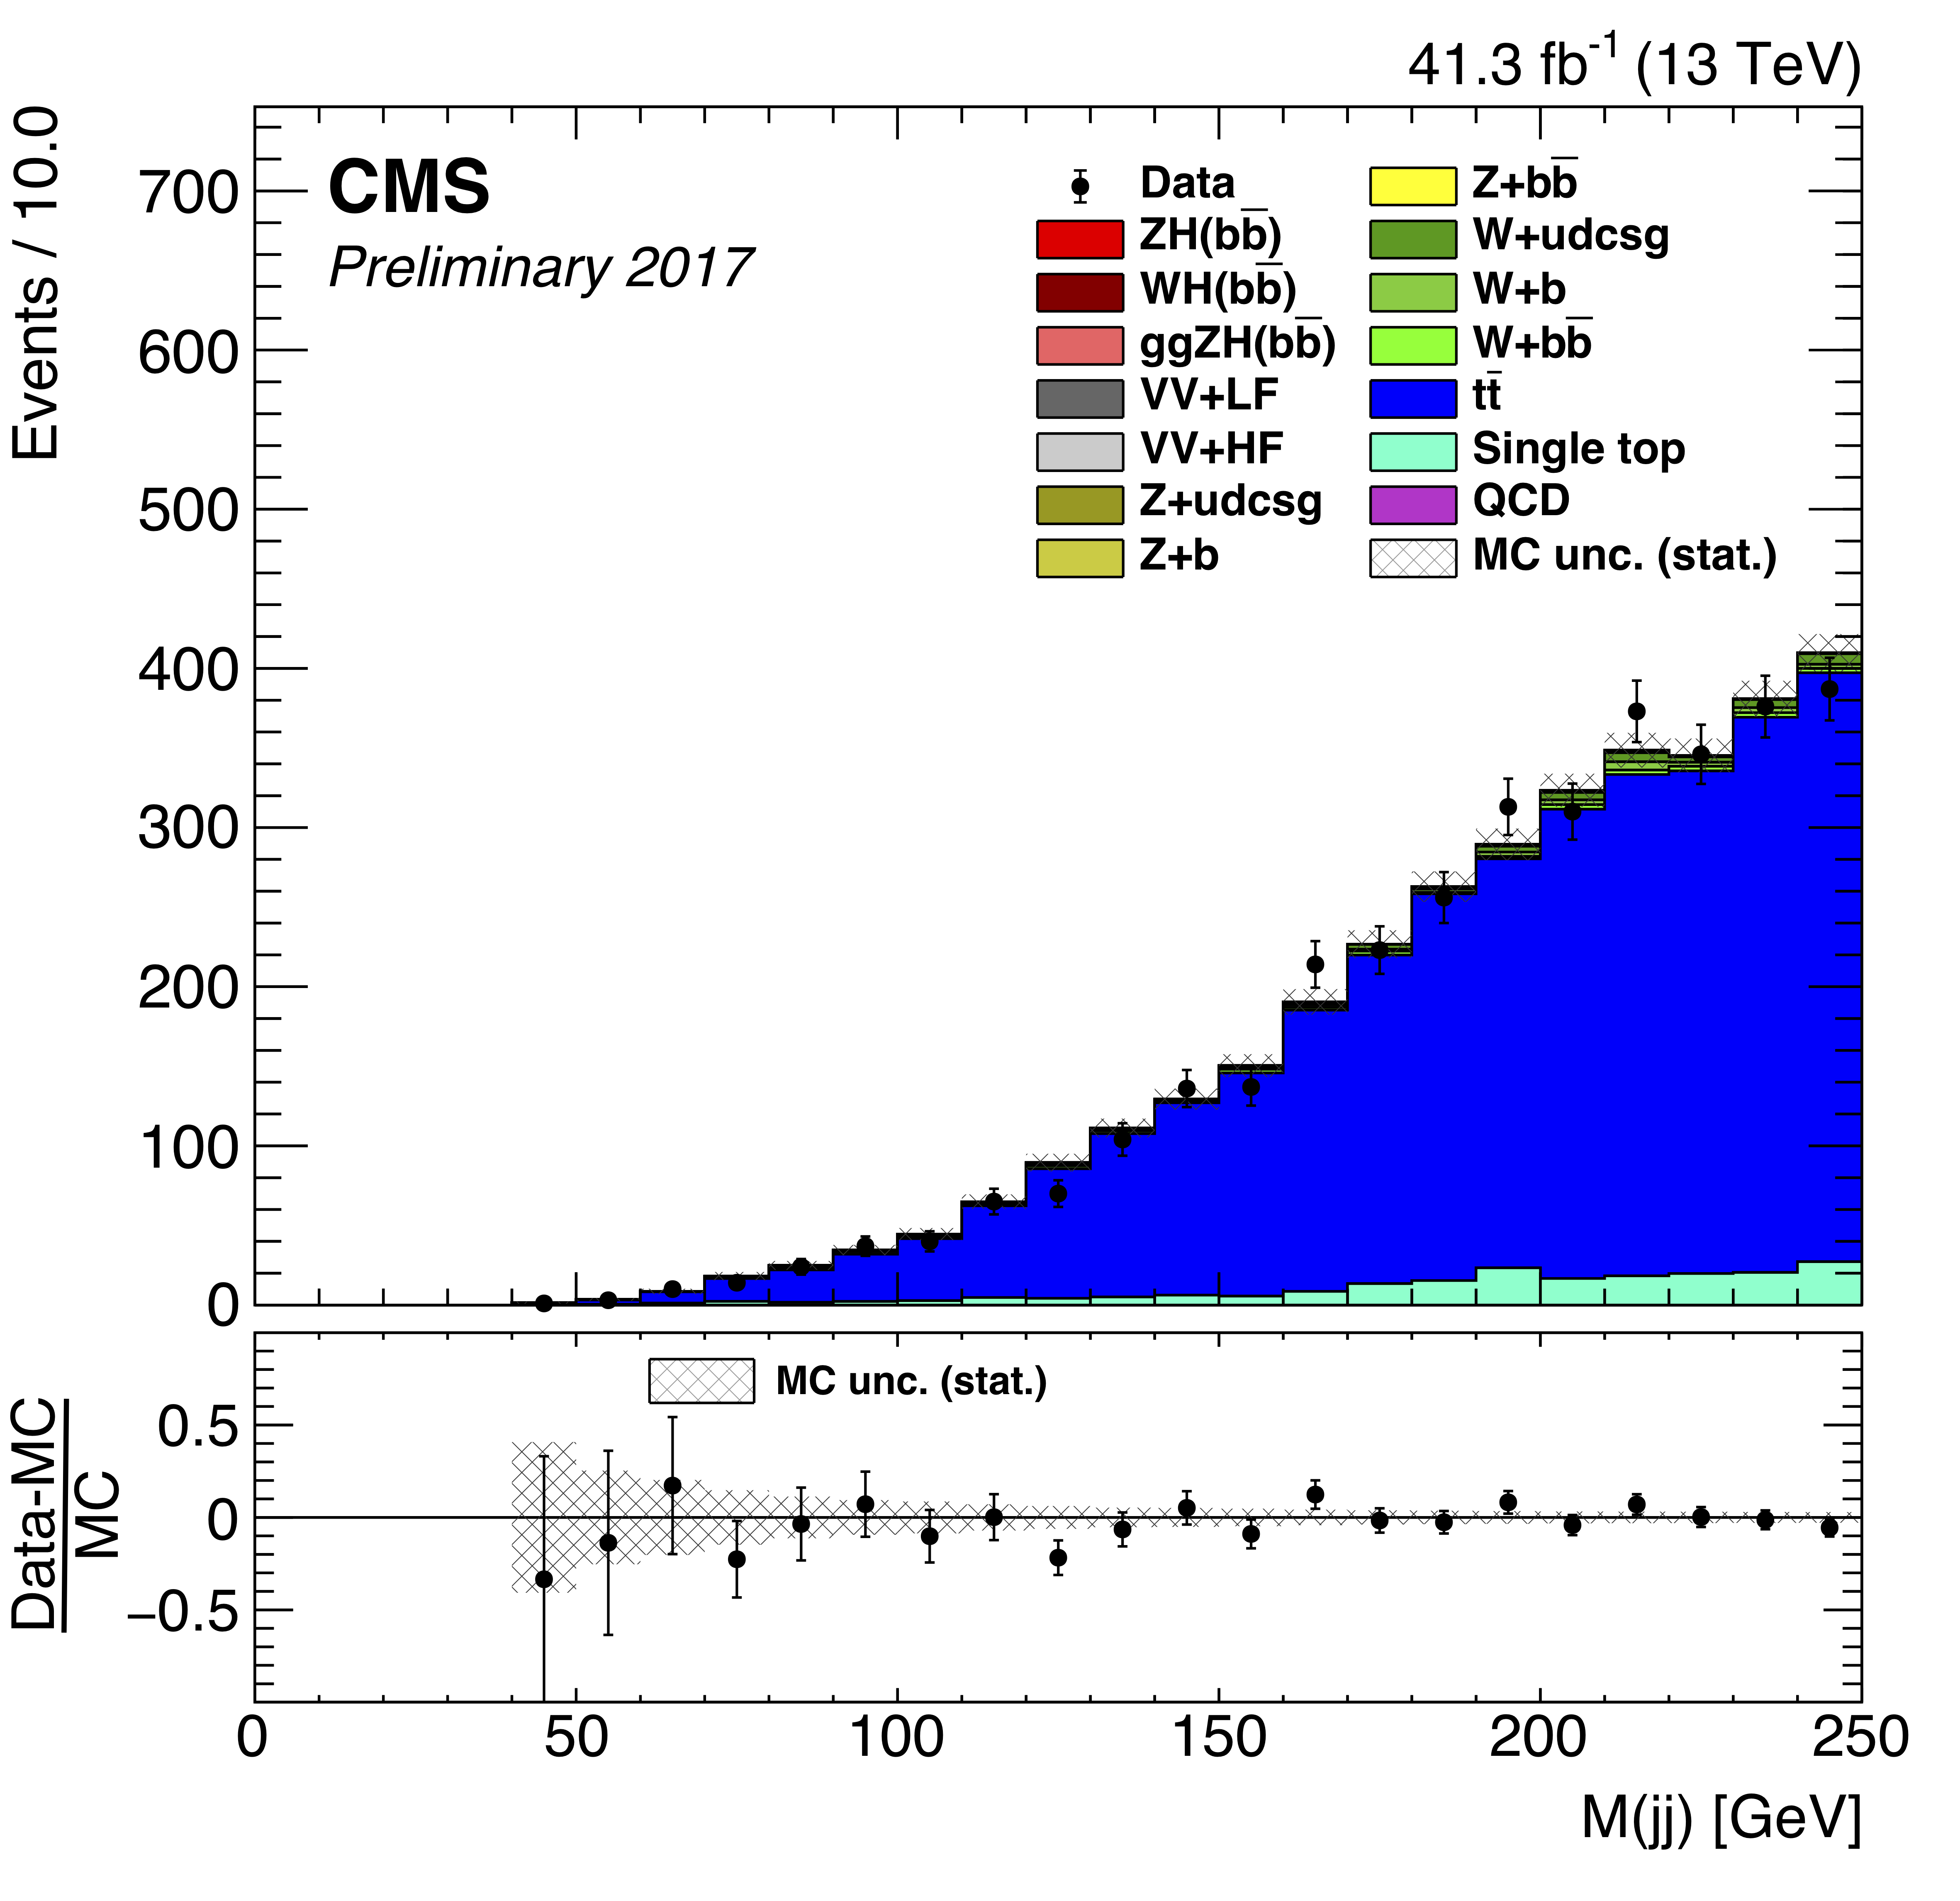
\includegraphics[width=0.39\linewidth]{images/CR_Znn_TT/H_mass}}
    \subfigure [] {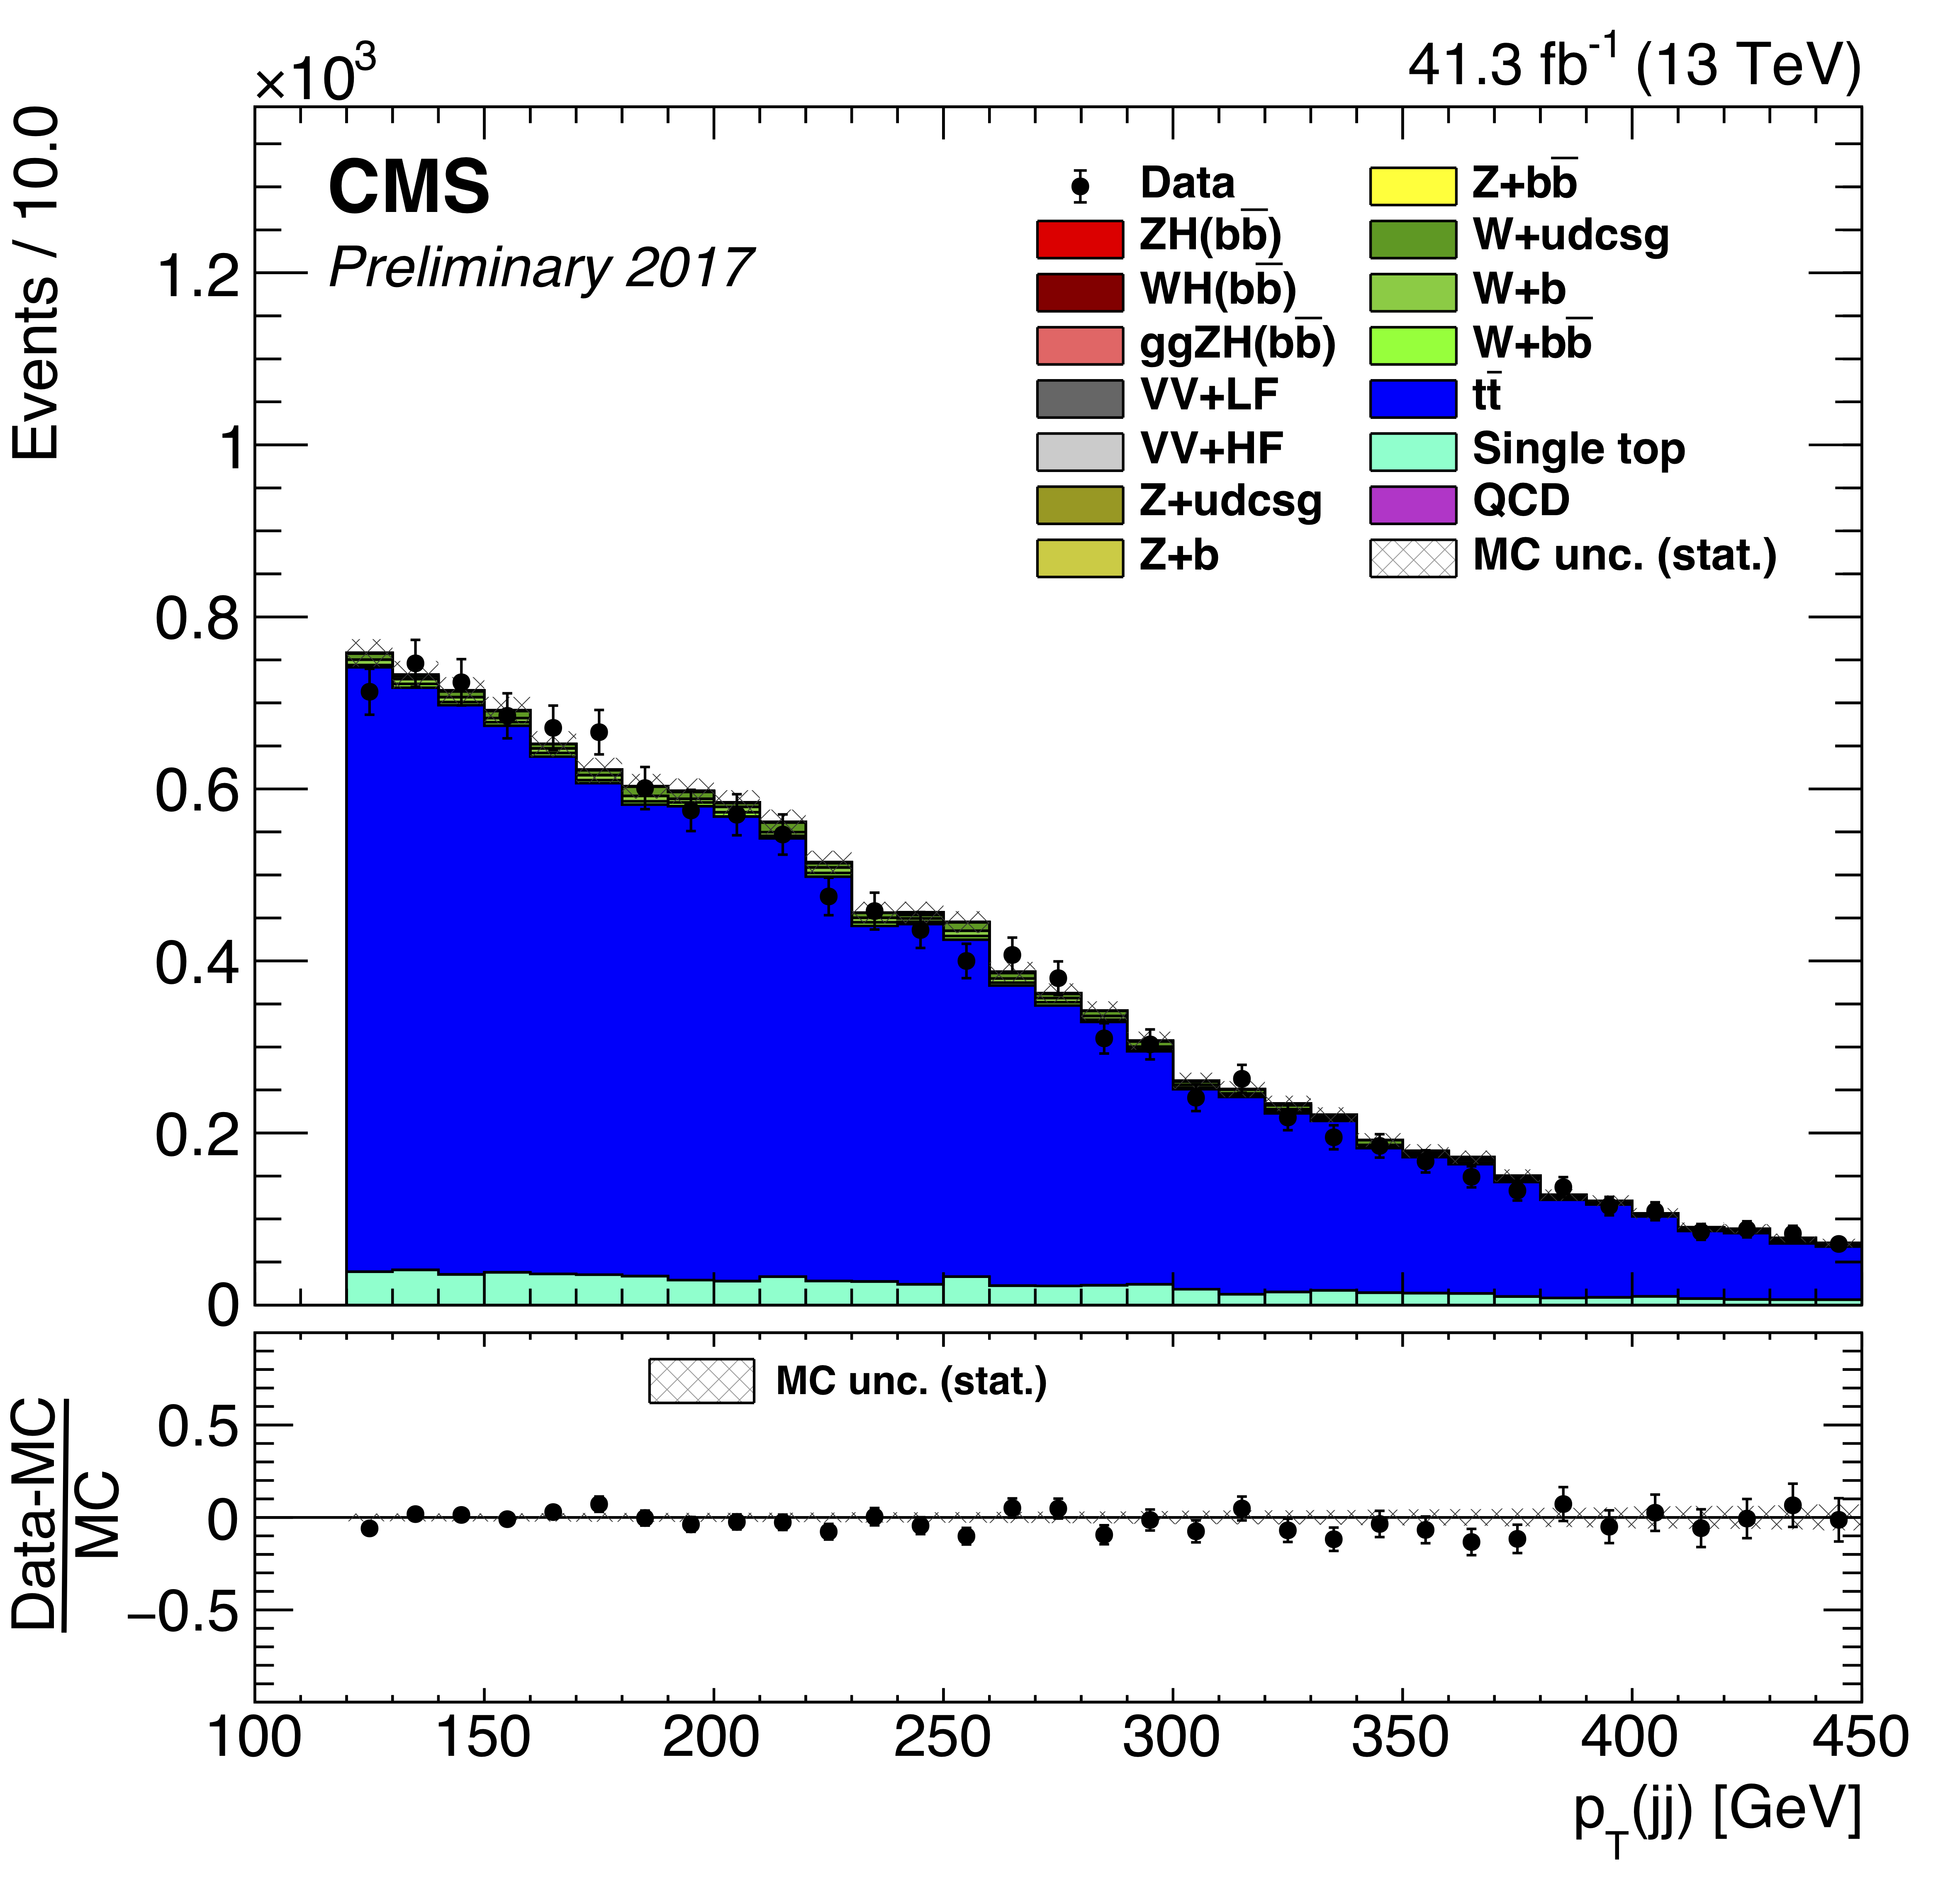
\includegraphics[width=0.39\linewidth]{images/CR_Znn_TT/H_pt}}
  }
  \mbox{
    \subfigure [] {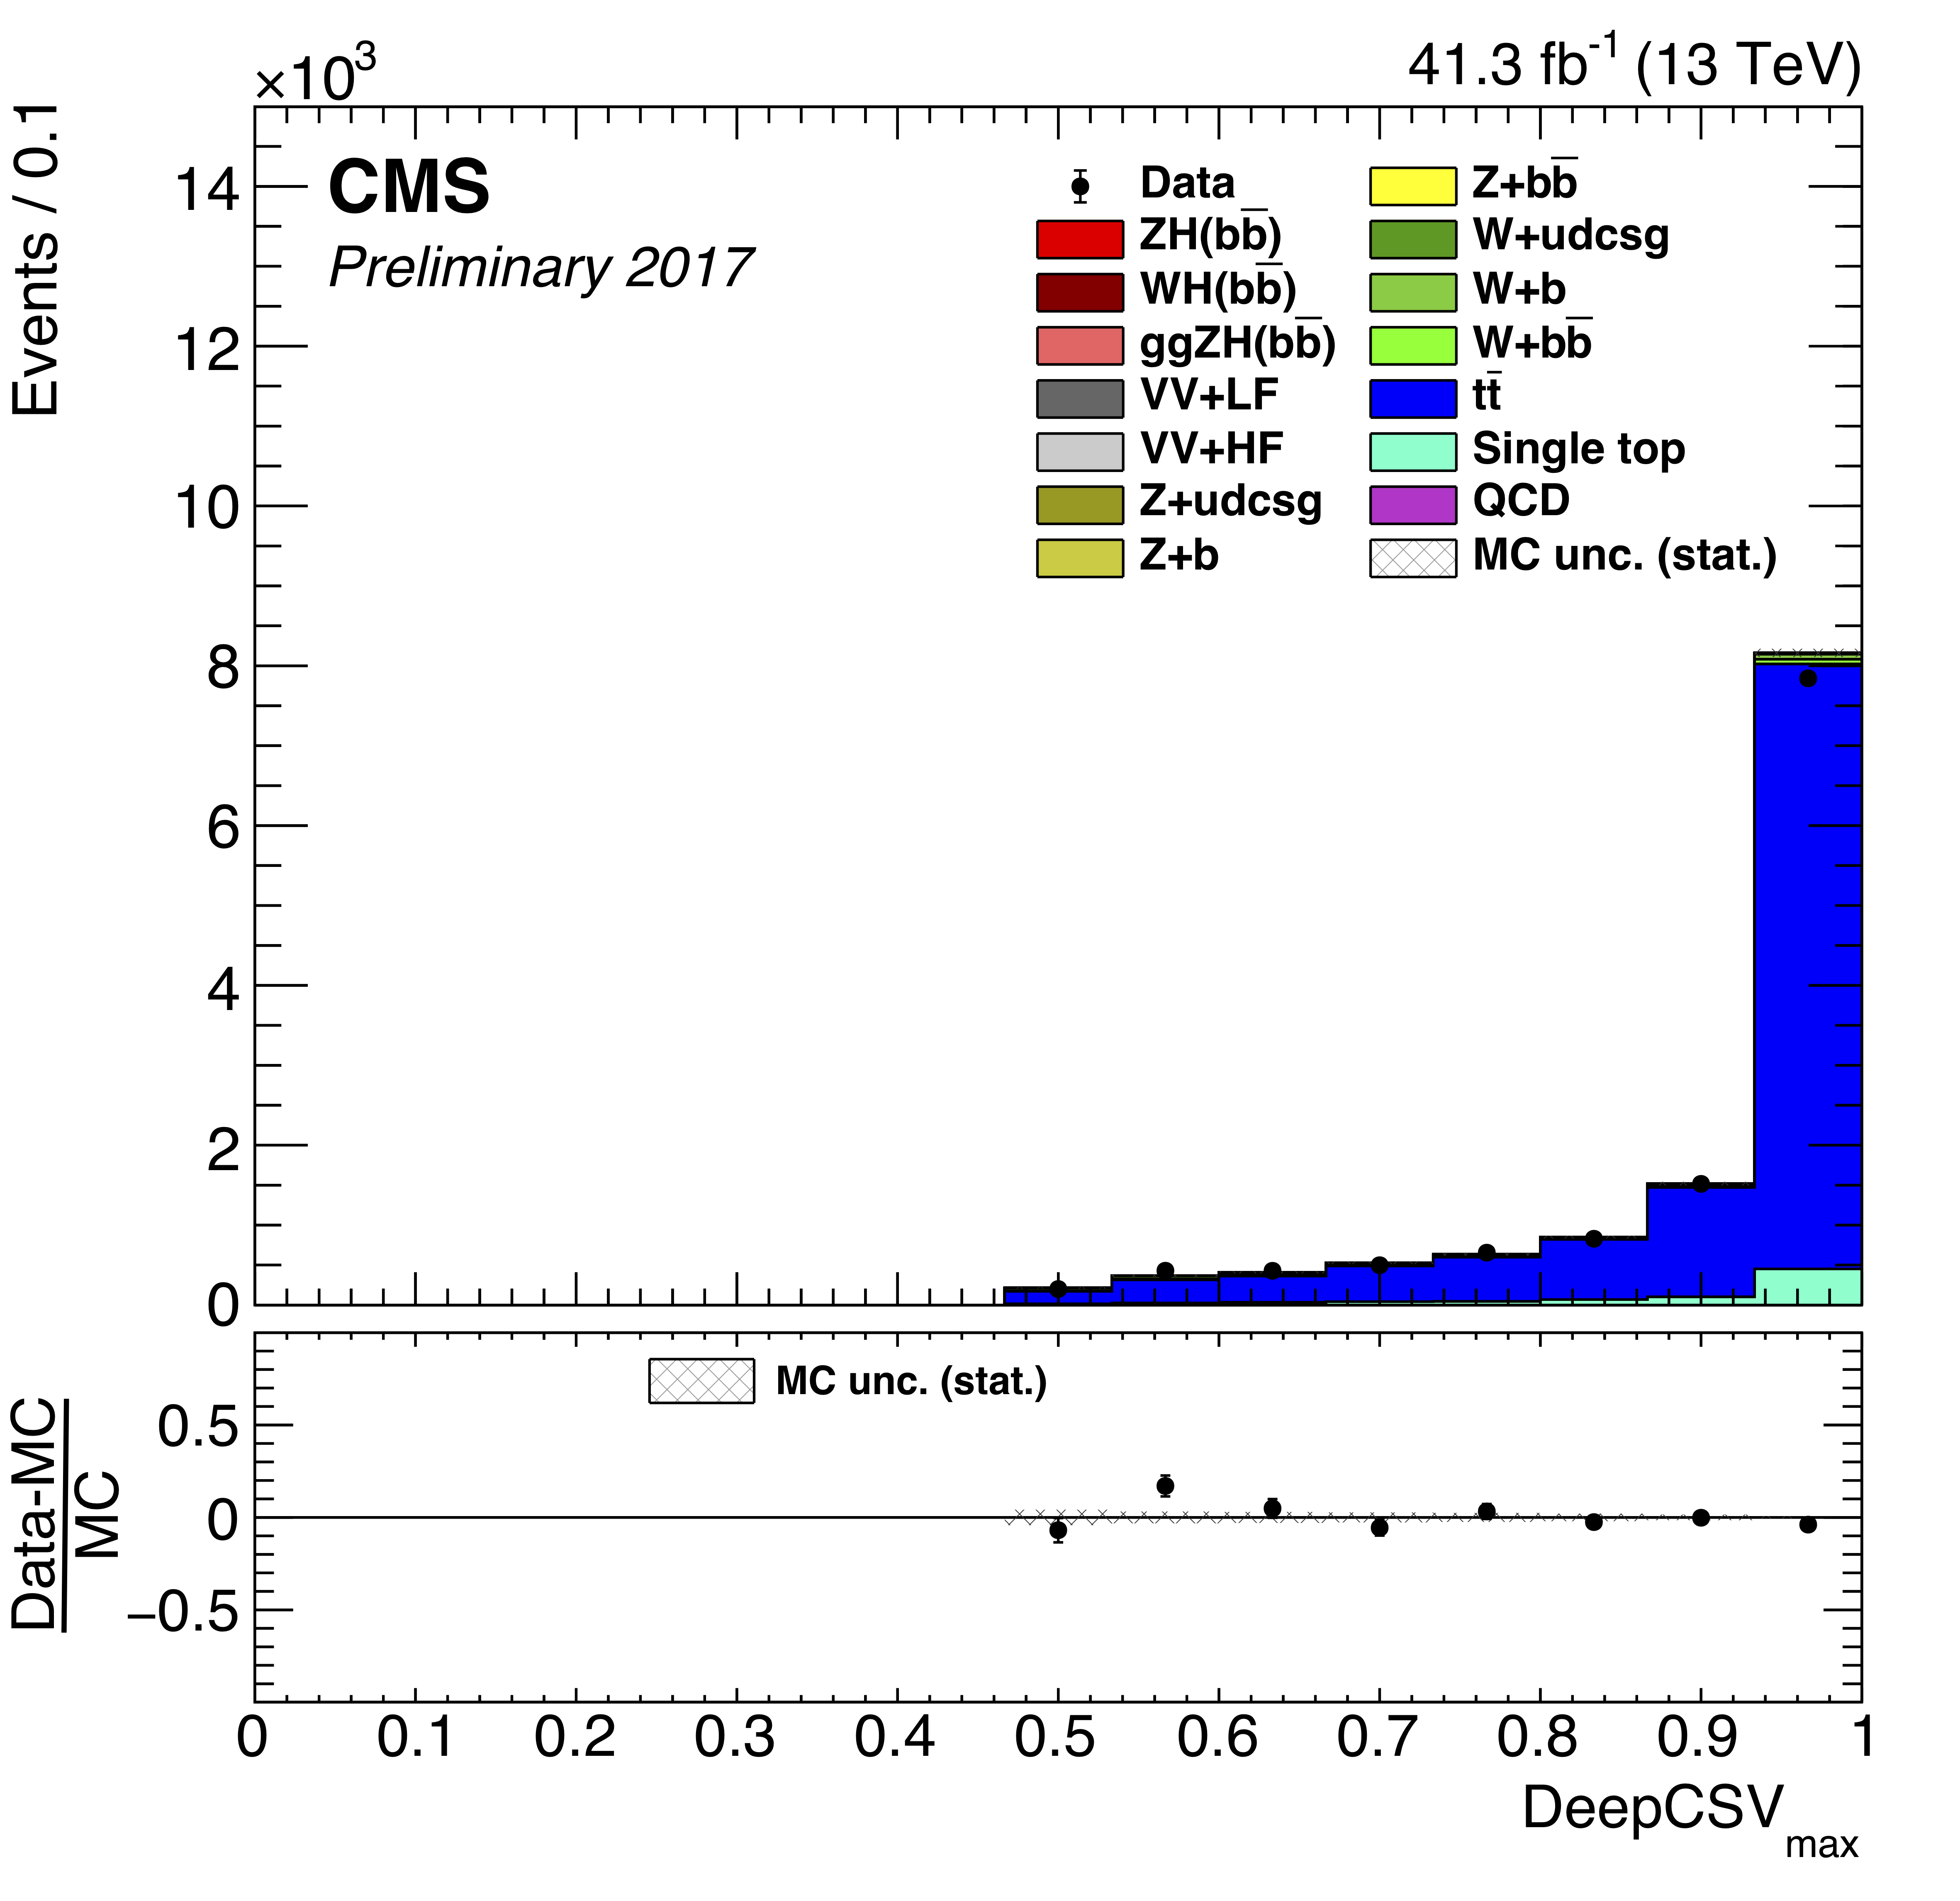
\includegraphics[width=0.39\linewidth]{images/CR_Znn_TT/hJets_DeepCSV_0}}
    \subfigure [] {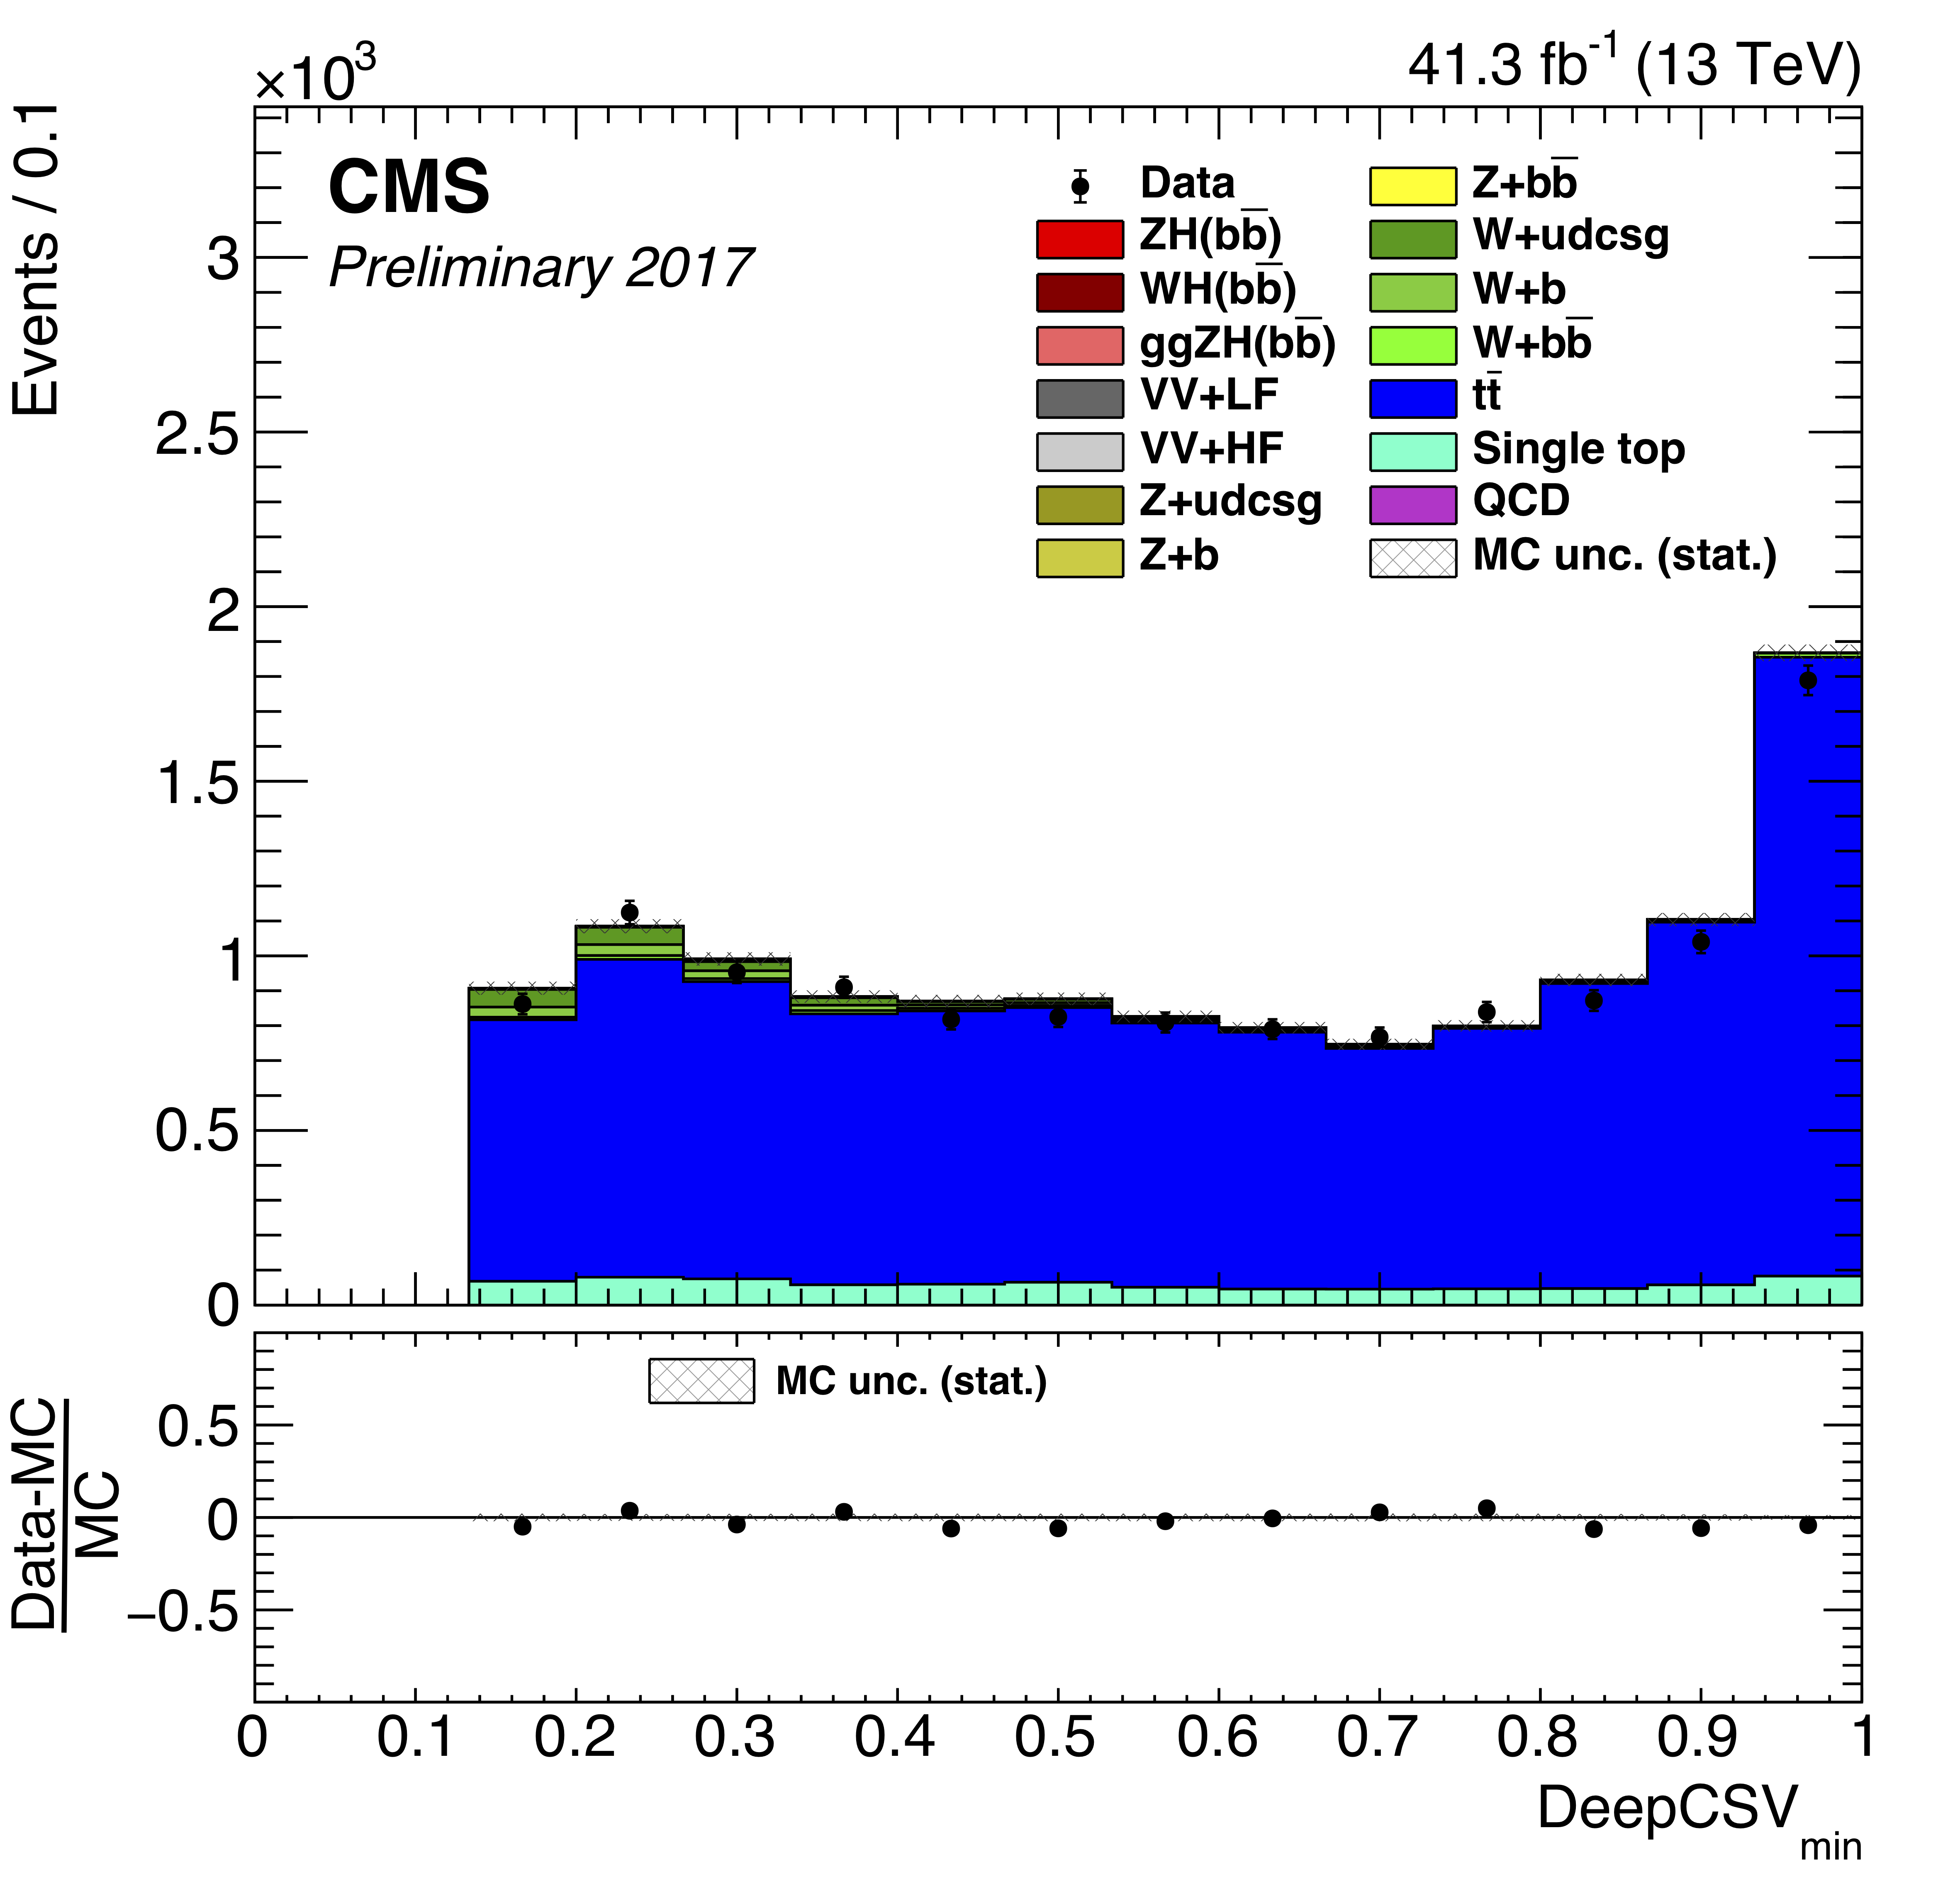
\includegraphics[width=0.39\linewidth]{images/CR_Znn_TT/hJets_DeepCSV_1}}
  }
  \mbox{
    \subfigure [] {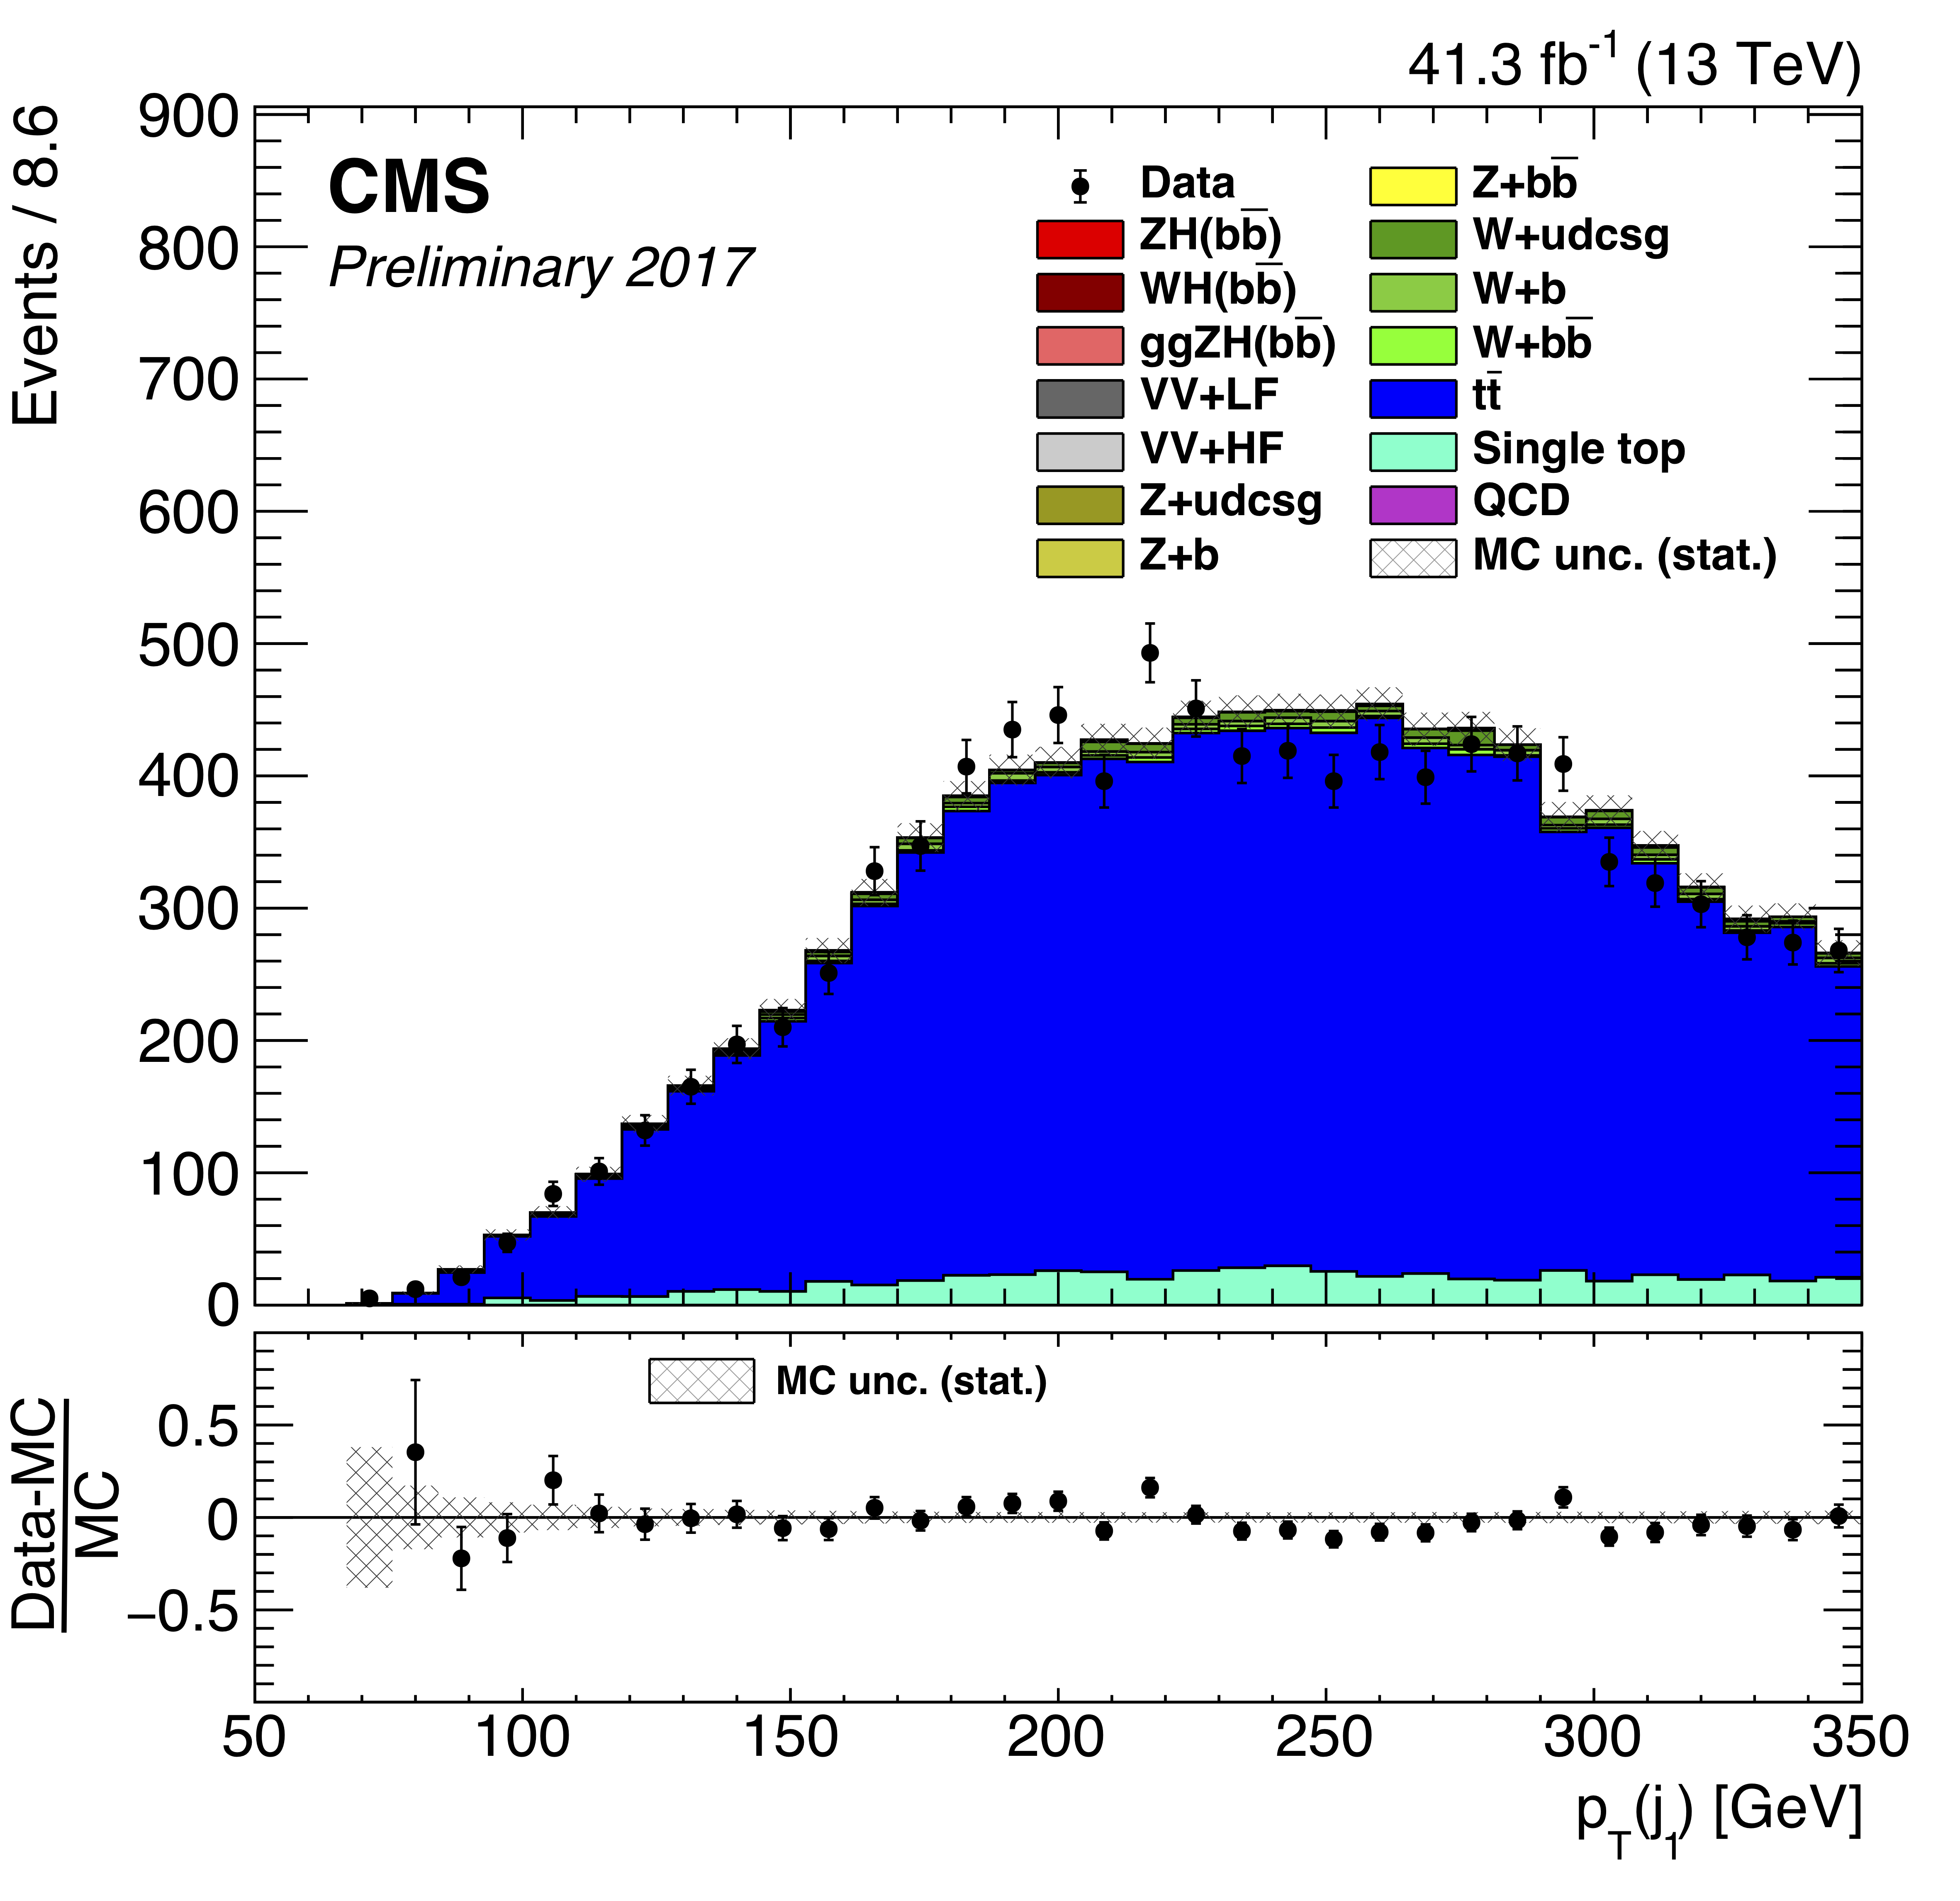
\includegraphics[width=0.39\linewidth]{images/CR_Znn_TT/hJets_leadingPt}}
    \subfigure [] {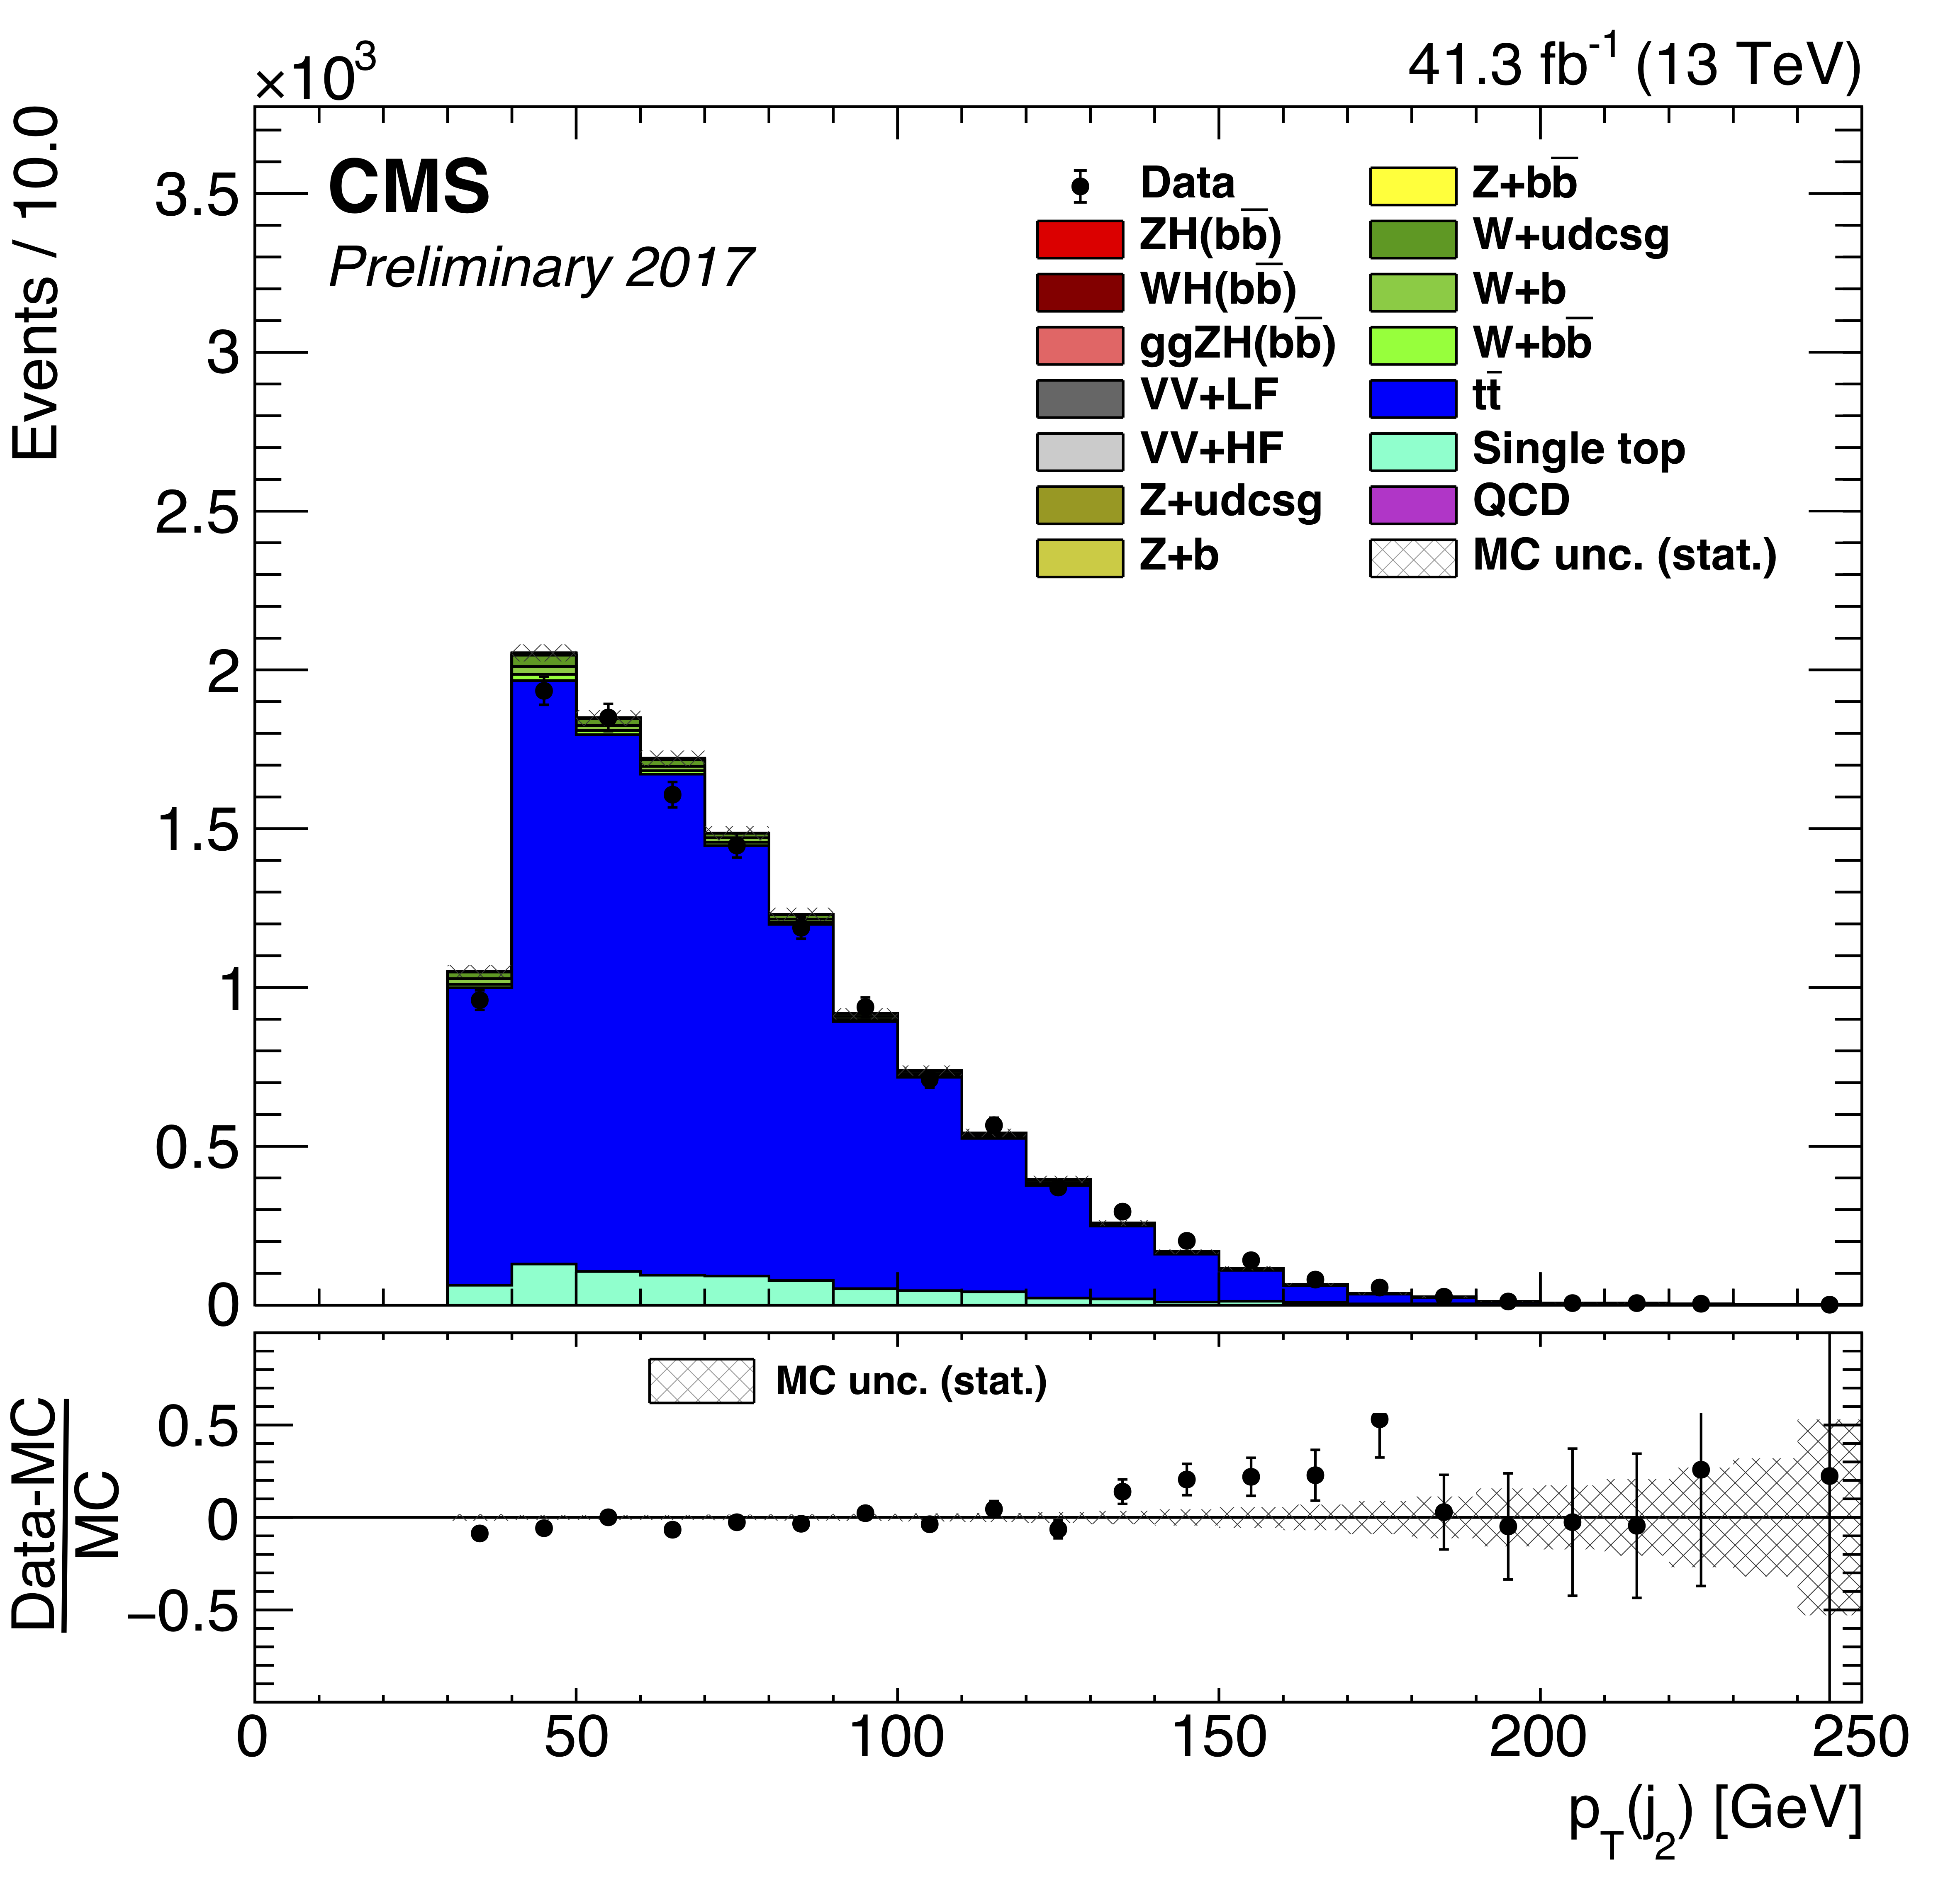
\includegraphics[width=0.39\linewidth]{images/CR_Znn_TT/hJets_subleadingPt}}
  }
  \caption[\qrkt\qrktbar\ Control Region Distributions for the \ZnnH\ Channel]{The distributions of variables in the \qrkt\qrktbar\ control region of the \ZnnH\ channel: A) $m(jj)$, B) $\pT(jj)$, C) \btagmax, D) \btagmin, E) \pTjmax, F) \pTjmin.}
  \label{fig:CR_Znn_TT_1}
\end{figure}

\clearpage

\begin{figure}[htbp]
  \centering
  \mbox{
    \subfigure [] {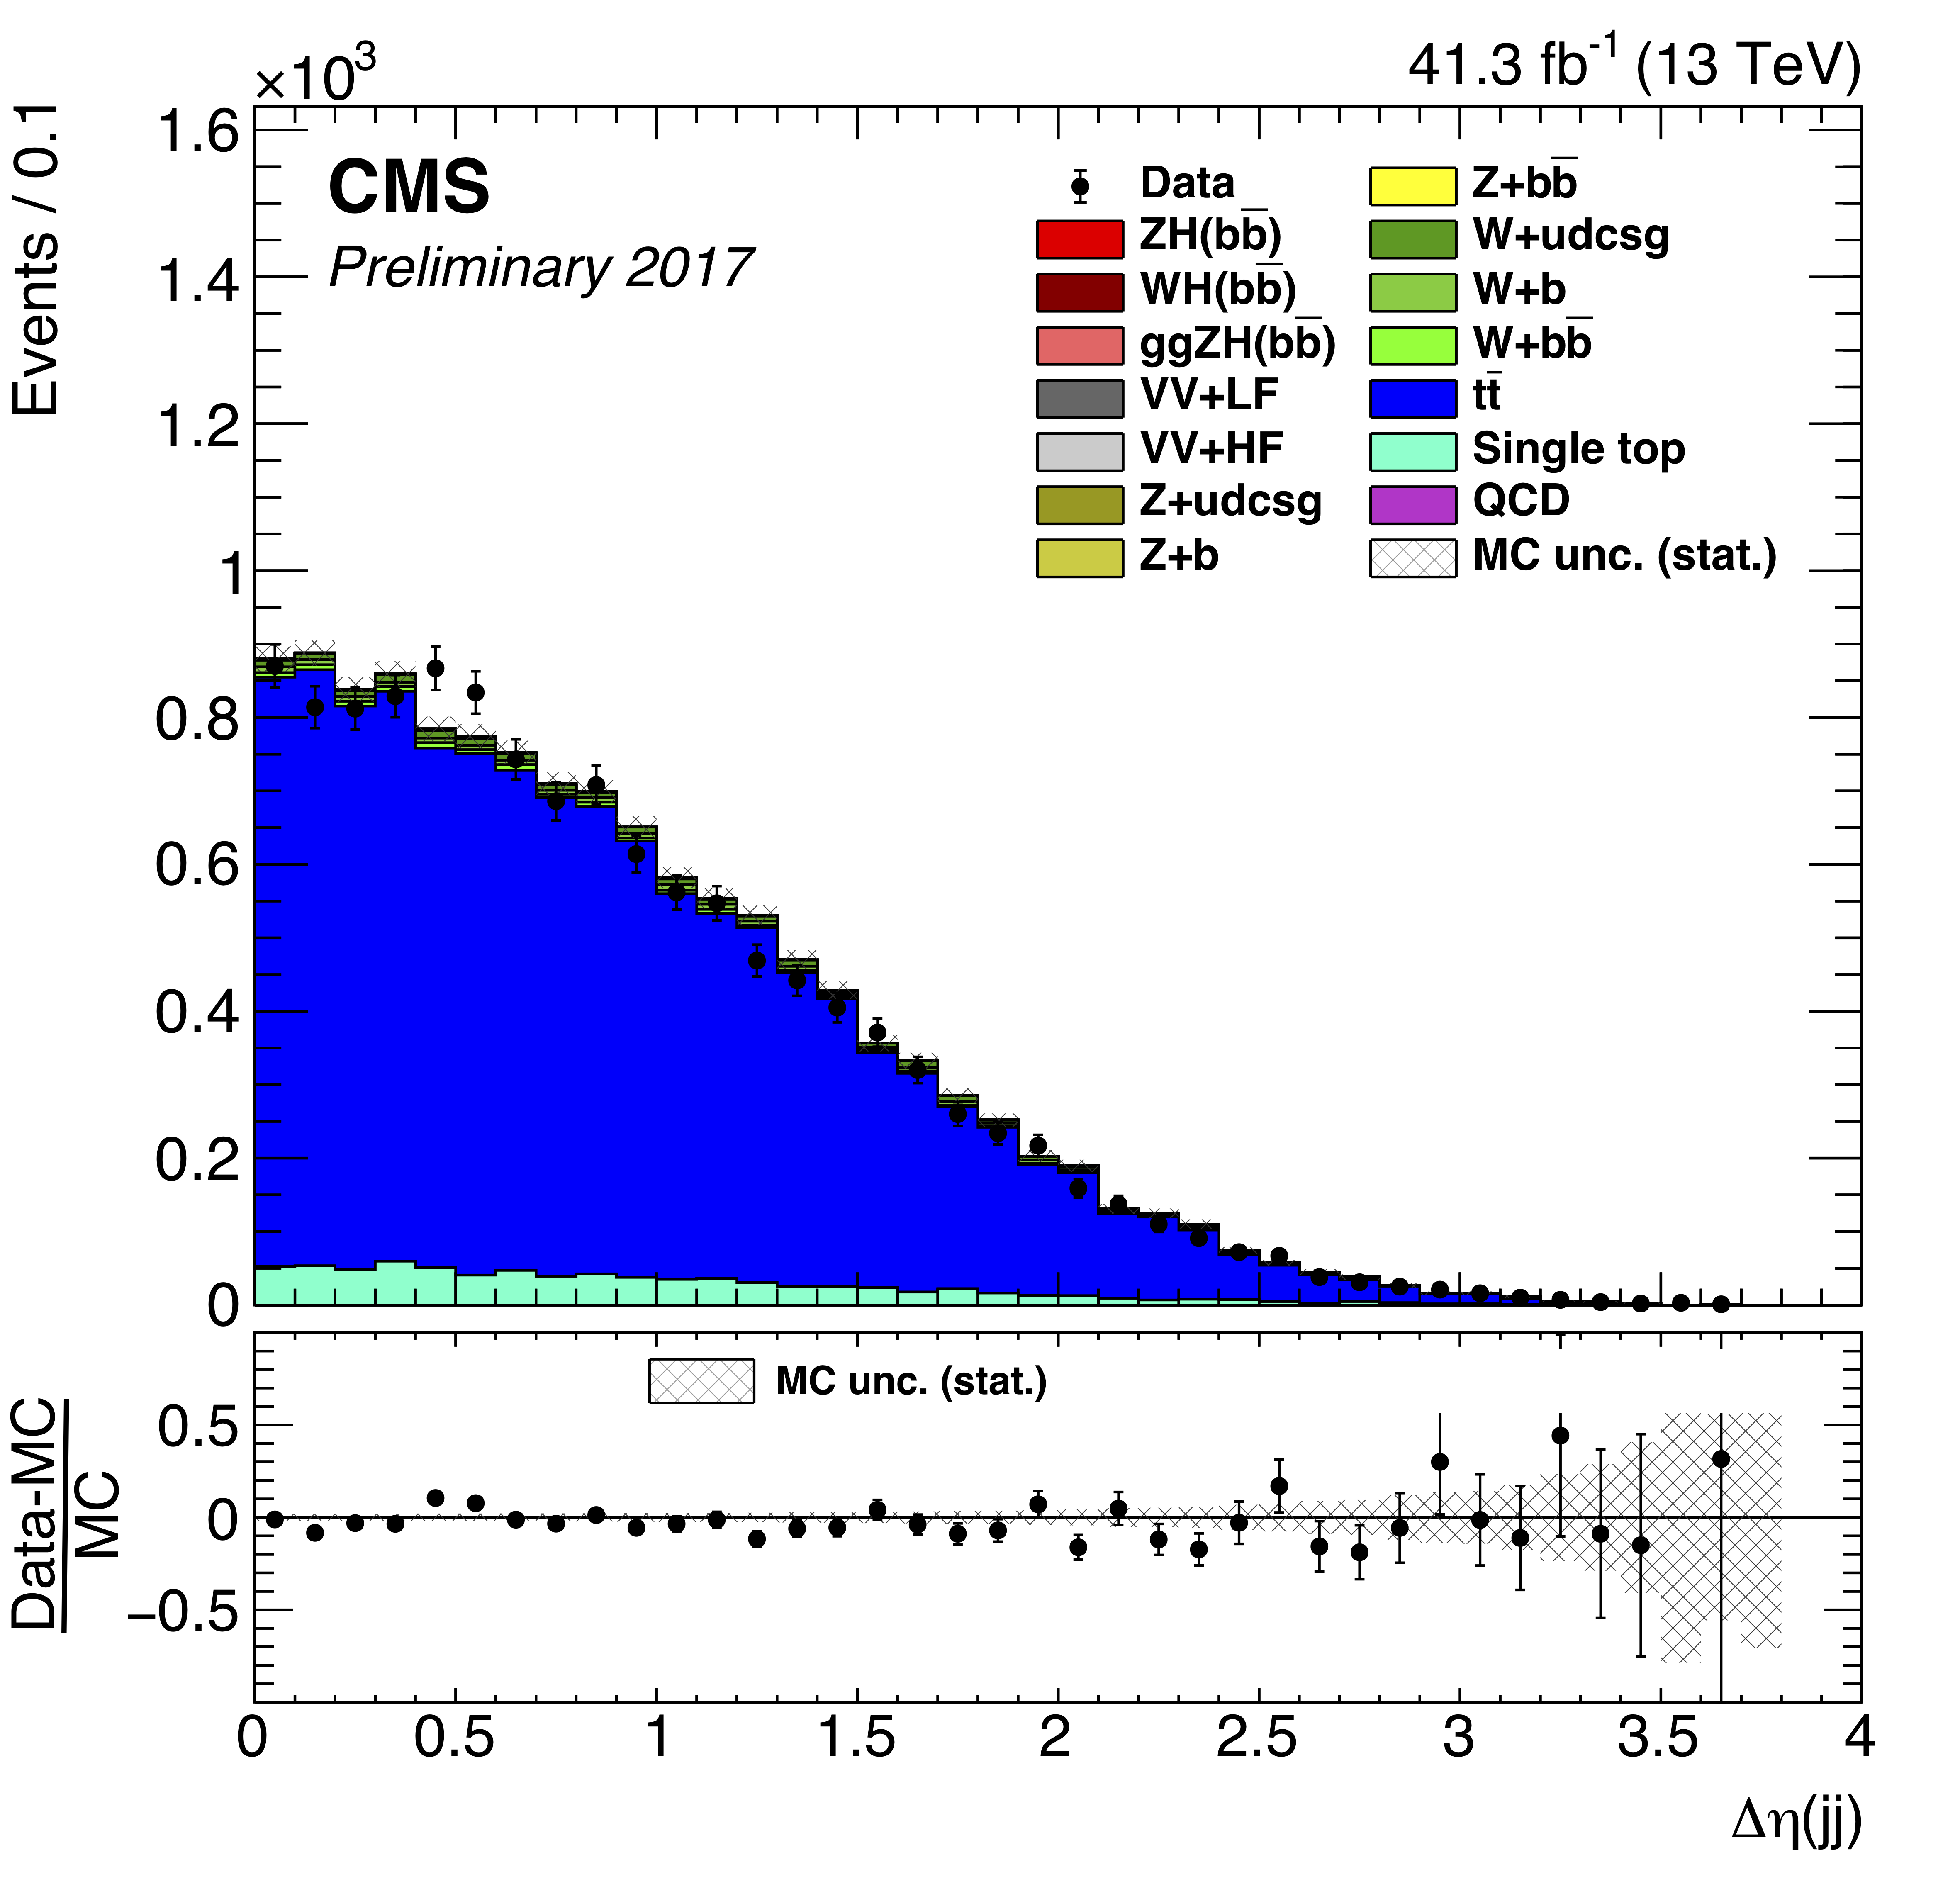
\includegraphics[width=0.39\linewidth]{images/CR_Znn_TT/HJ1_HJ2_dEta}}
    \subfigure [] {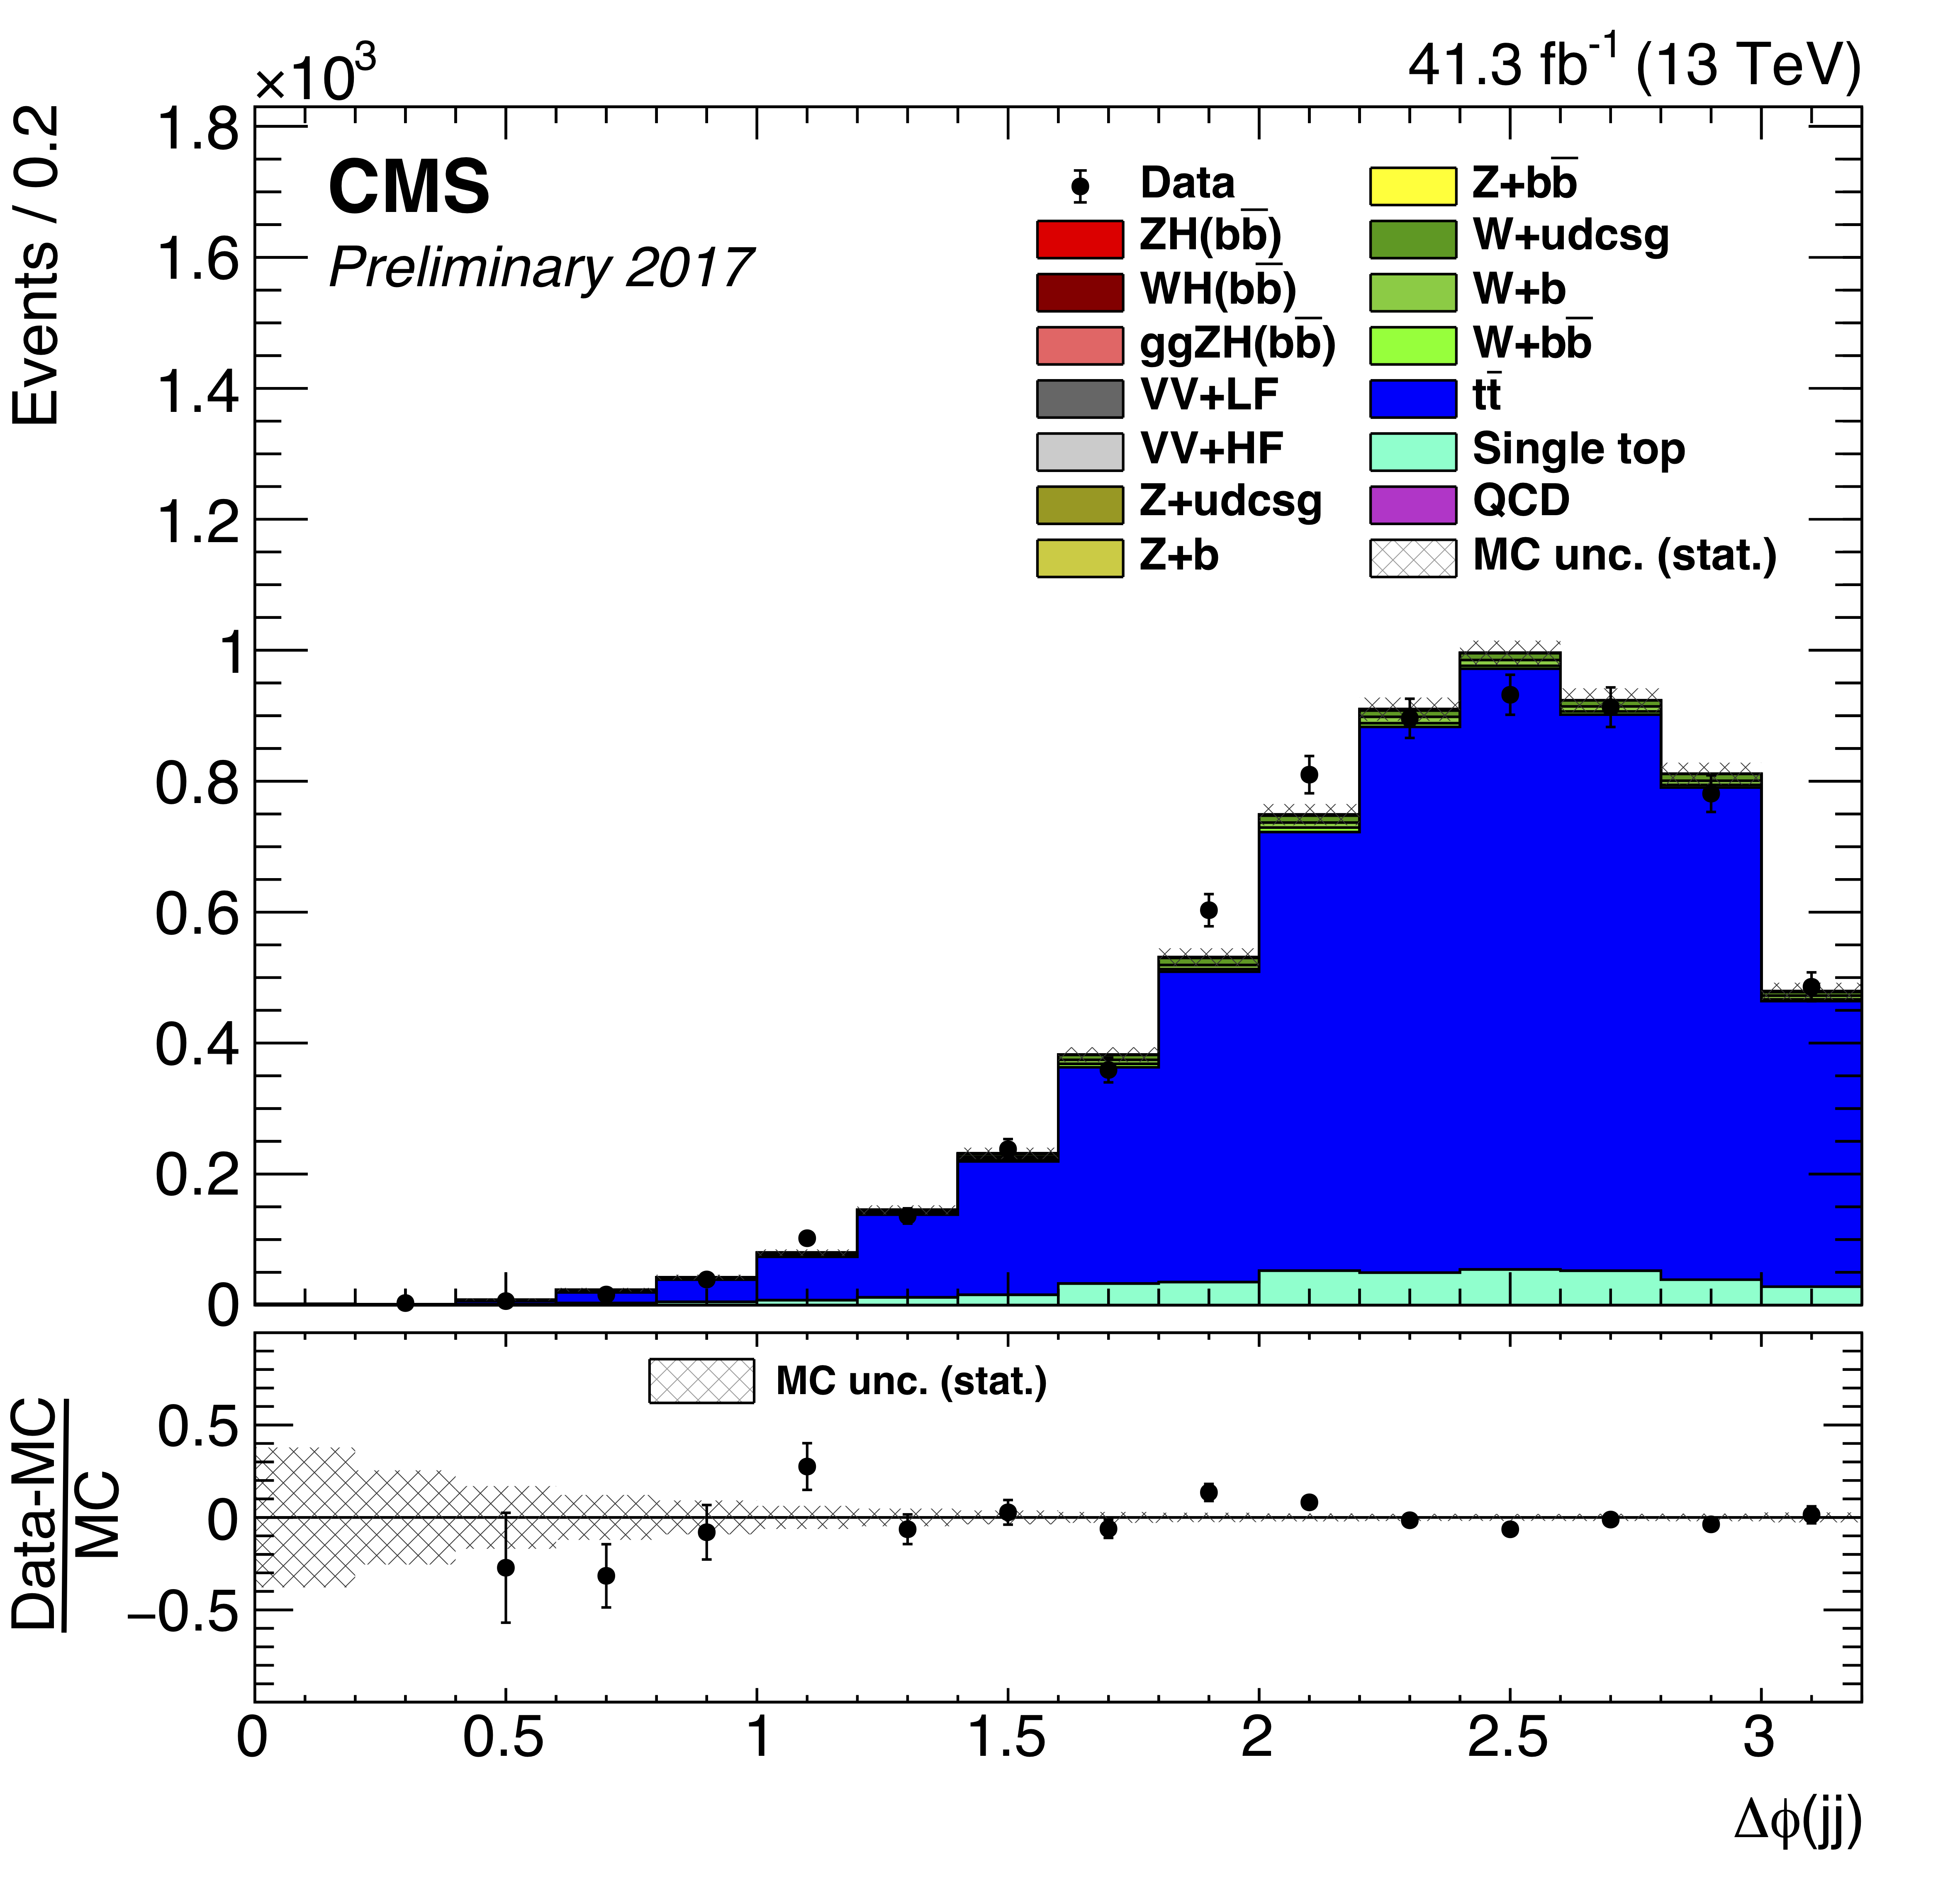
\includegraphics[width=0.39\linewidth]{images/CR_Znn_TT/HJ1_HJ2_dPhi}}
  }
  \mbox{
    \subfigure [] {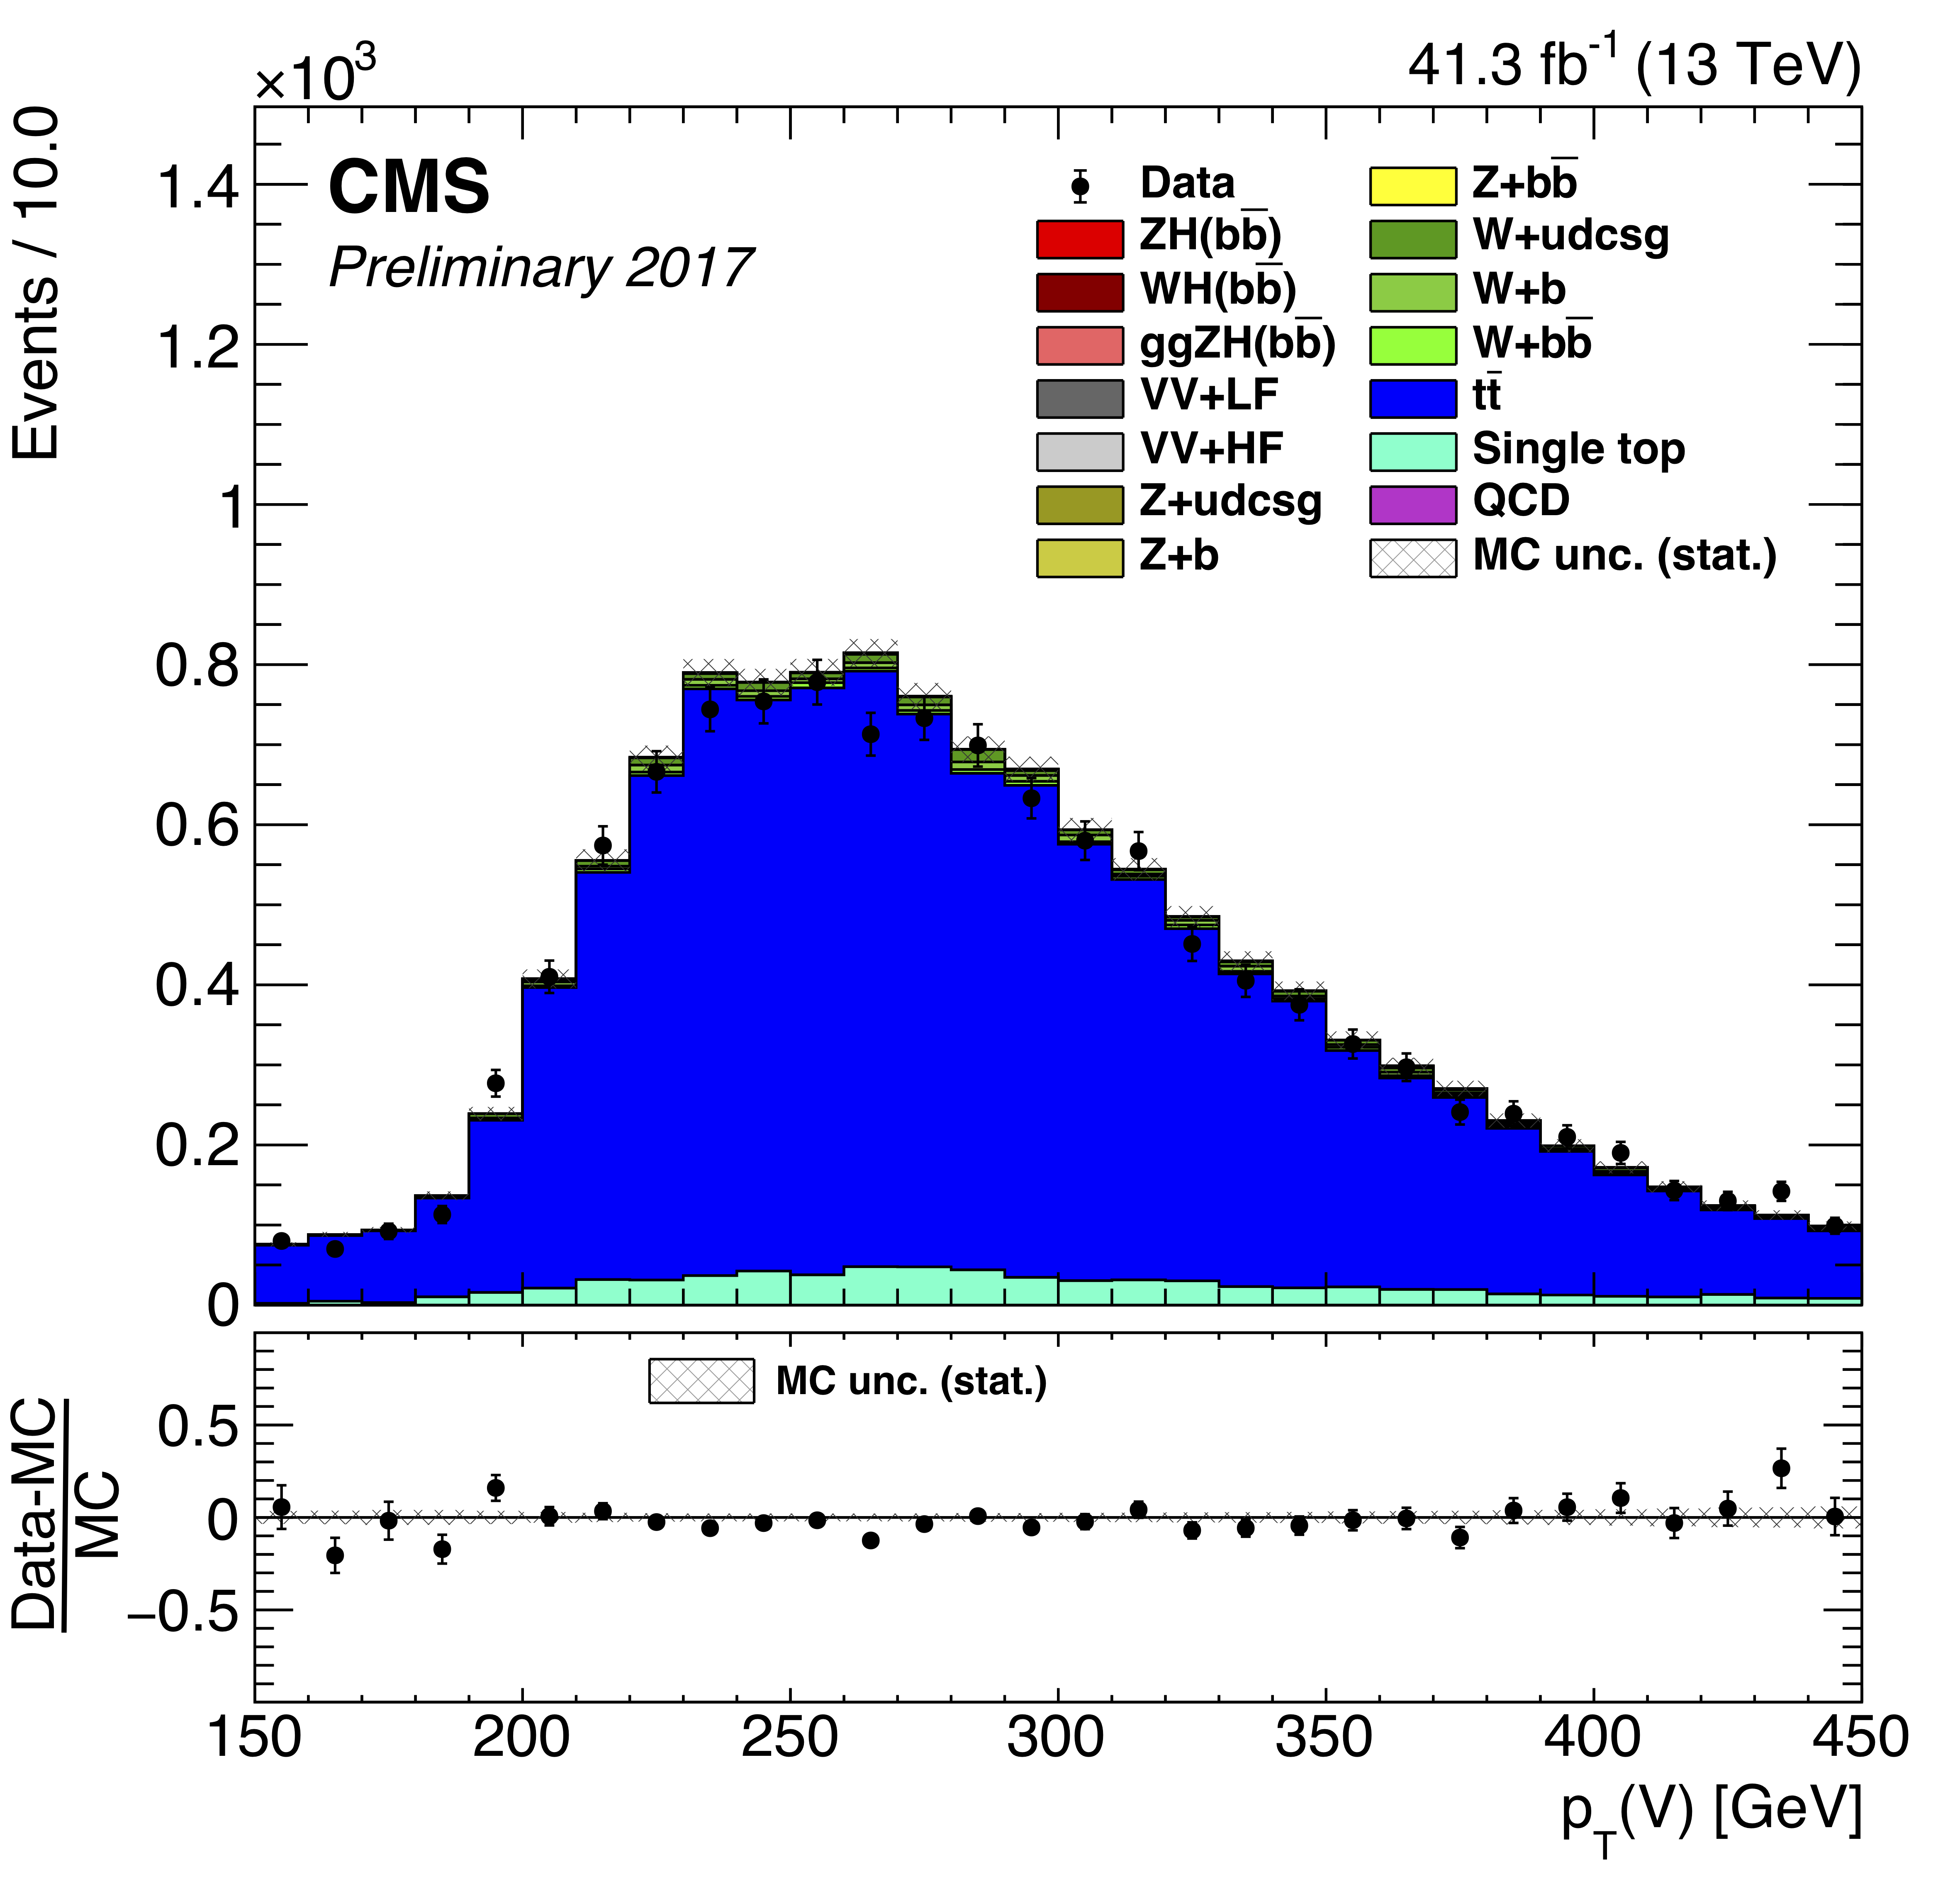
\includegraphics[width=0.39\linewidth]{images/CR_Znn_TT/V_pt}}
    \subfigure [] {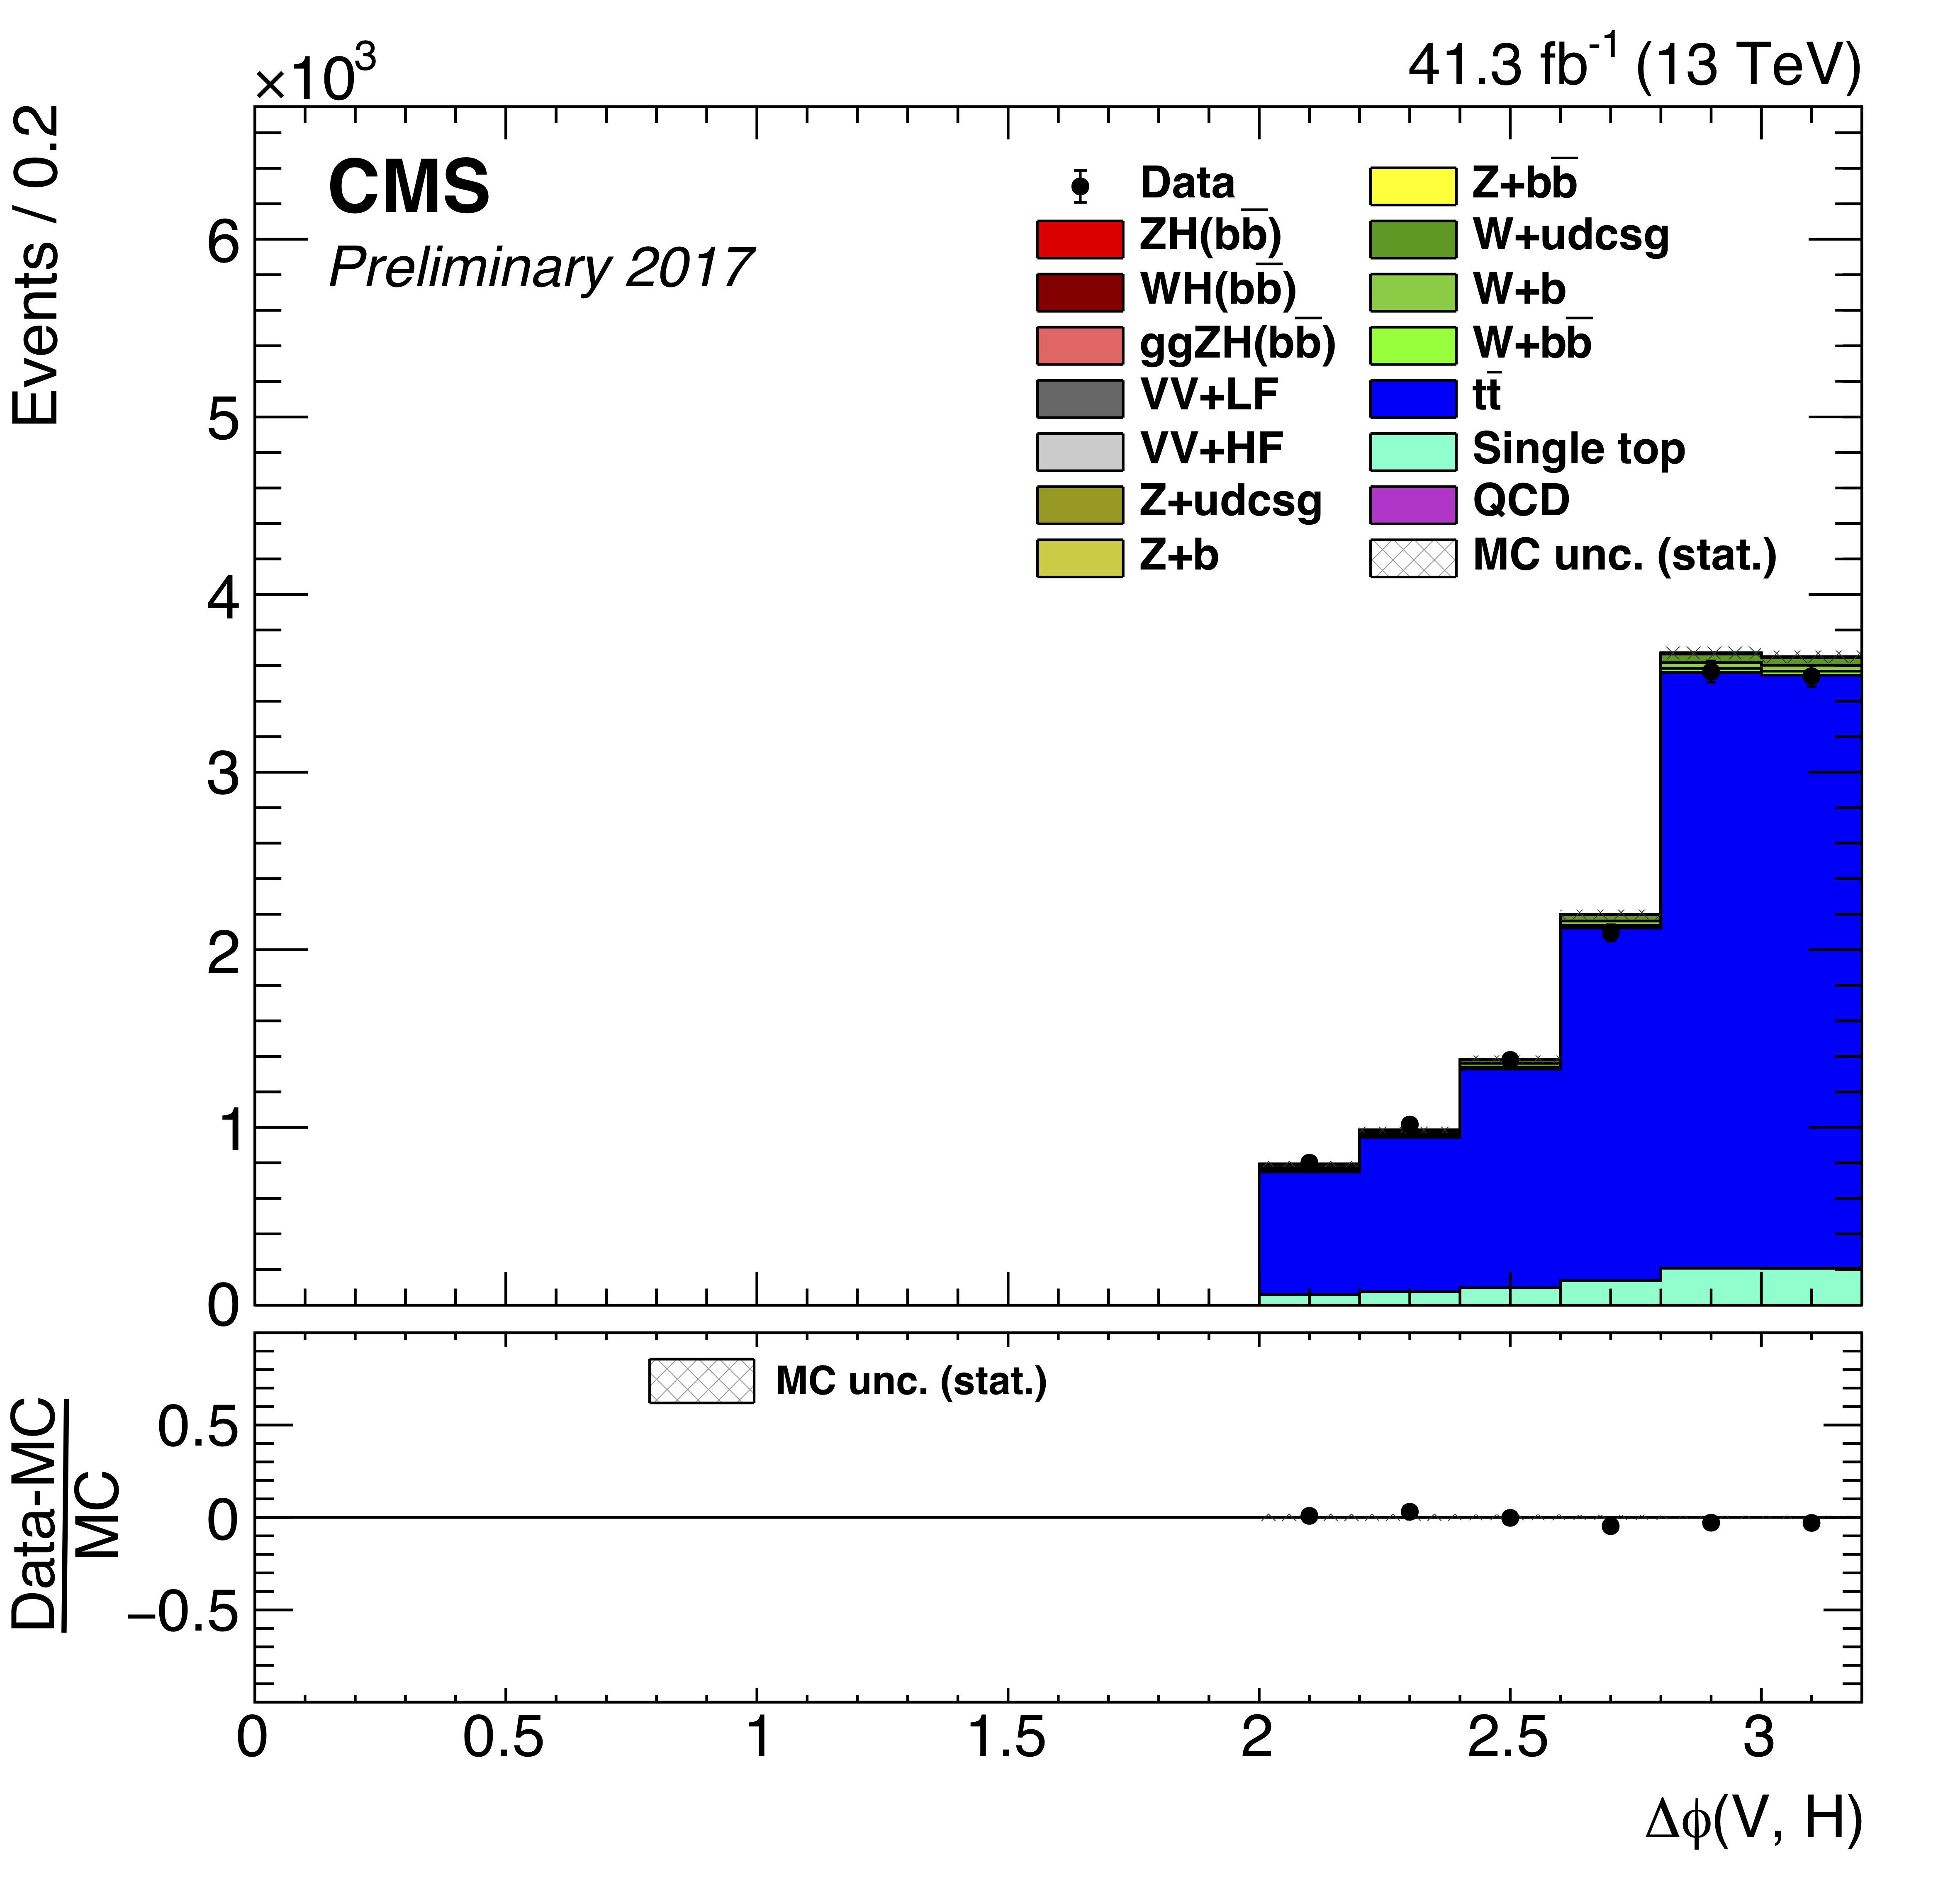
\includegraphics[width=0.39\linewidth]{images/CR_Znn_TT/HVdPhi}}
  }
  \mbox{
    \subfigure [] {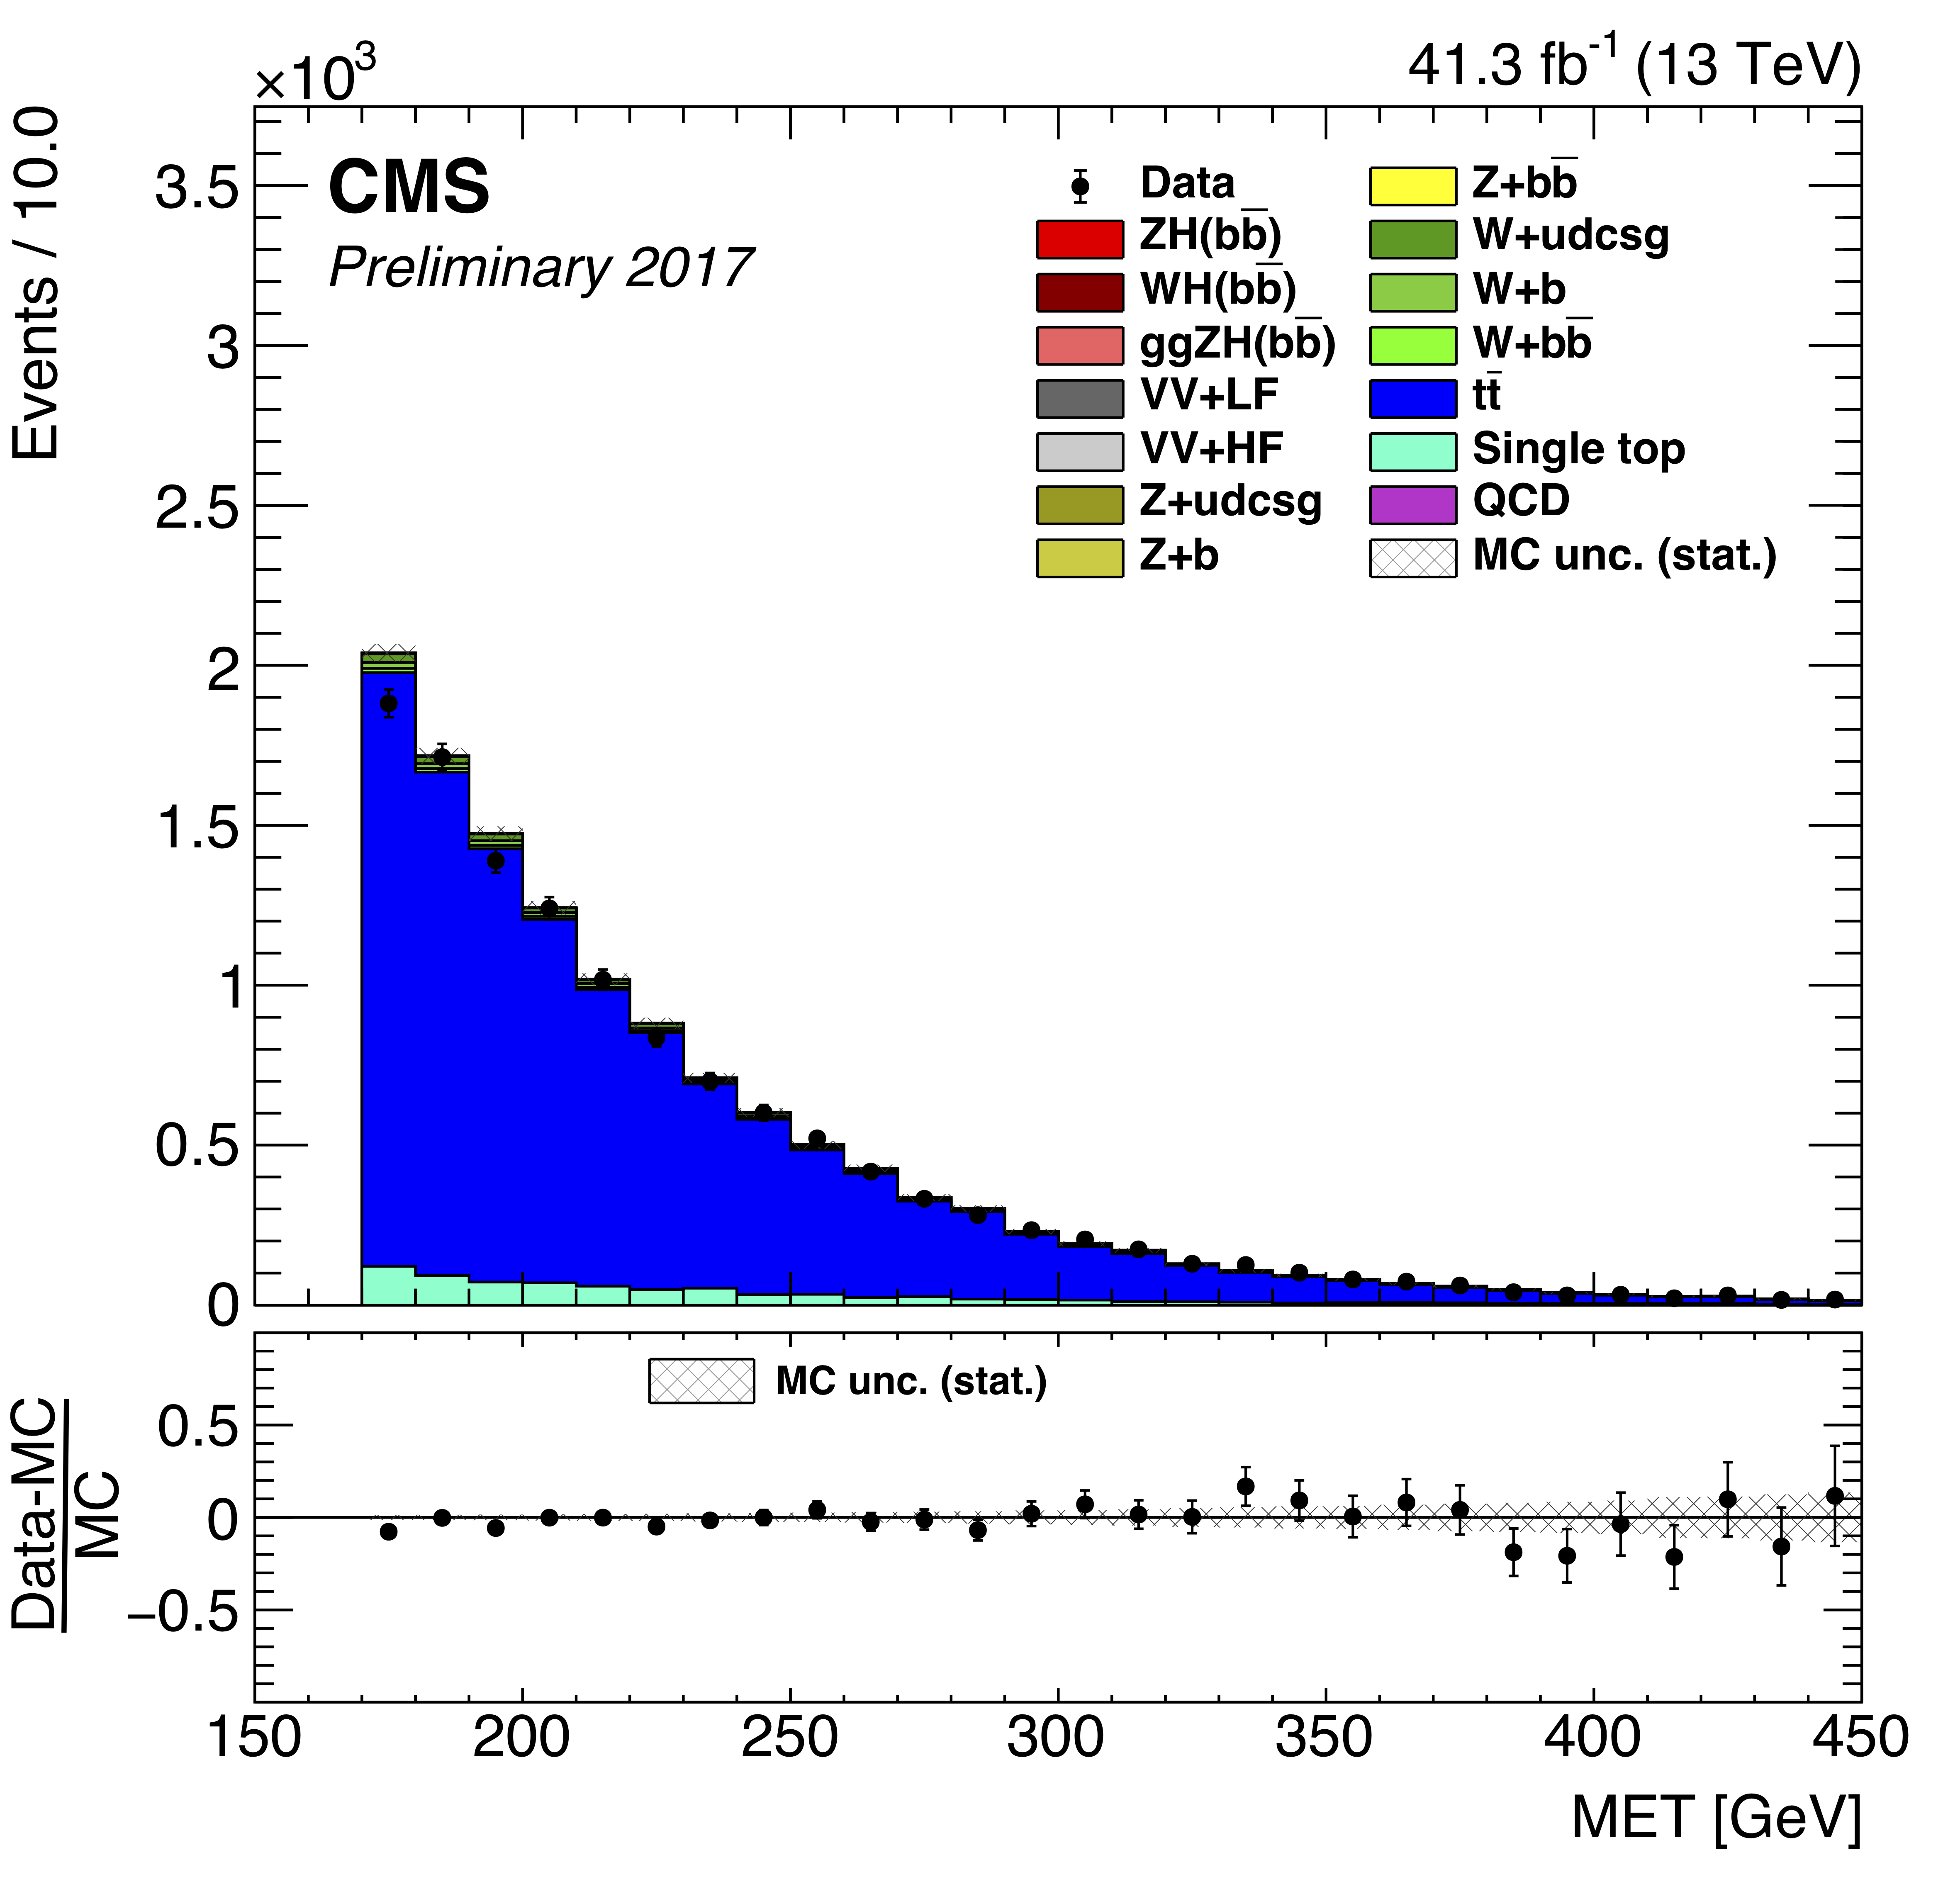
\includegraphics[width=0.39\linewidth]{images/CR_Znn_TT/MET_Pt}}
    \subfigure [] {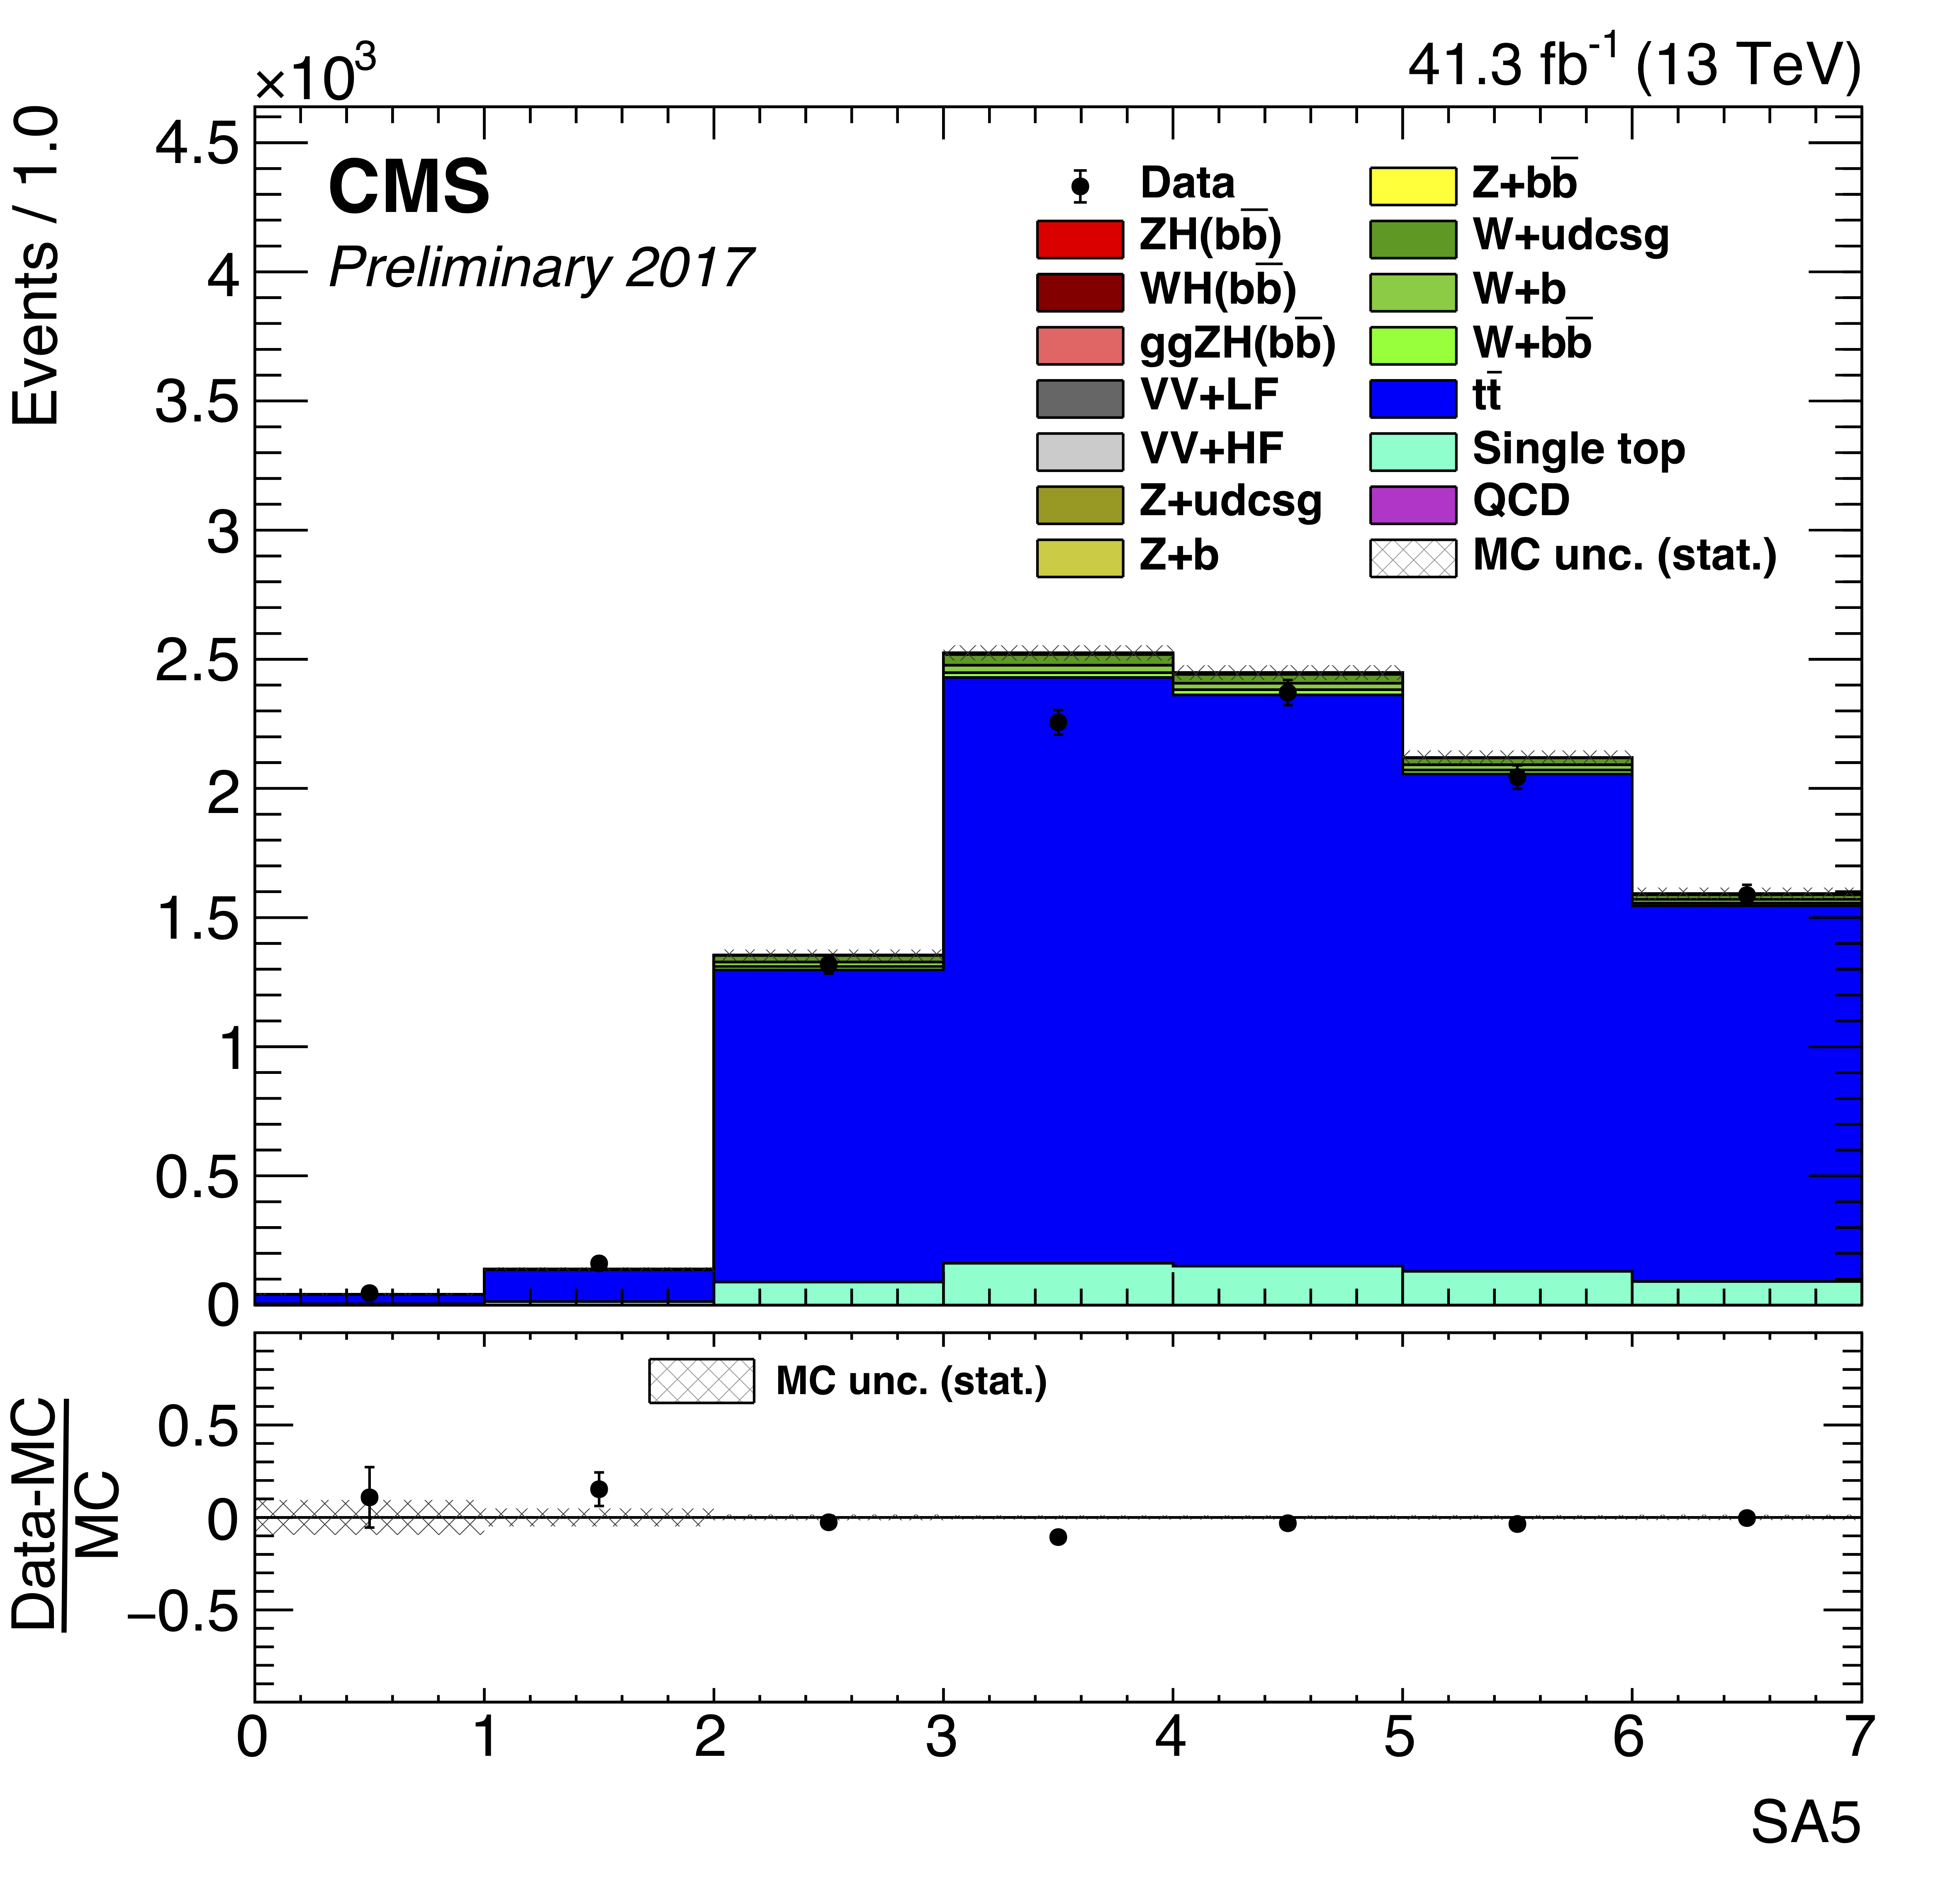
\includegraphics[width=0.39\linewidth]{images/CR_Znn_TT/SA5}}
  }
  \caption[Additional \qrkt\qrktbar\ Control Region Distributions for the \ZnnH\ Channel]{The distributions of variables in the \qrkt\qrktbar\ control region of the \ZnnH\ channel: A) $\left| \Delta \eta (j_{1}, j_{2}) \right|$, B) $\left| \Delta \phi (j_{1}, j_{2}) \right|$, C) $\pT(\bosV)$, D) $\left| \Delta \phi (\bosV, \bosH) \right|$, E) \pTmiss, F) SA5.}
  \label{fig:CR_Znn_TT_2}
\end{figure}

\clearpage

% Z+light

\begin{figure}[htbp]
  \centering
  \mbox{
    \subfigure [] {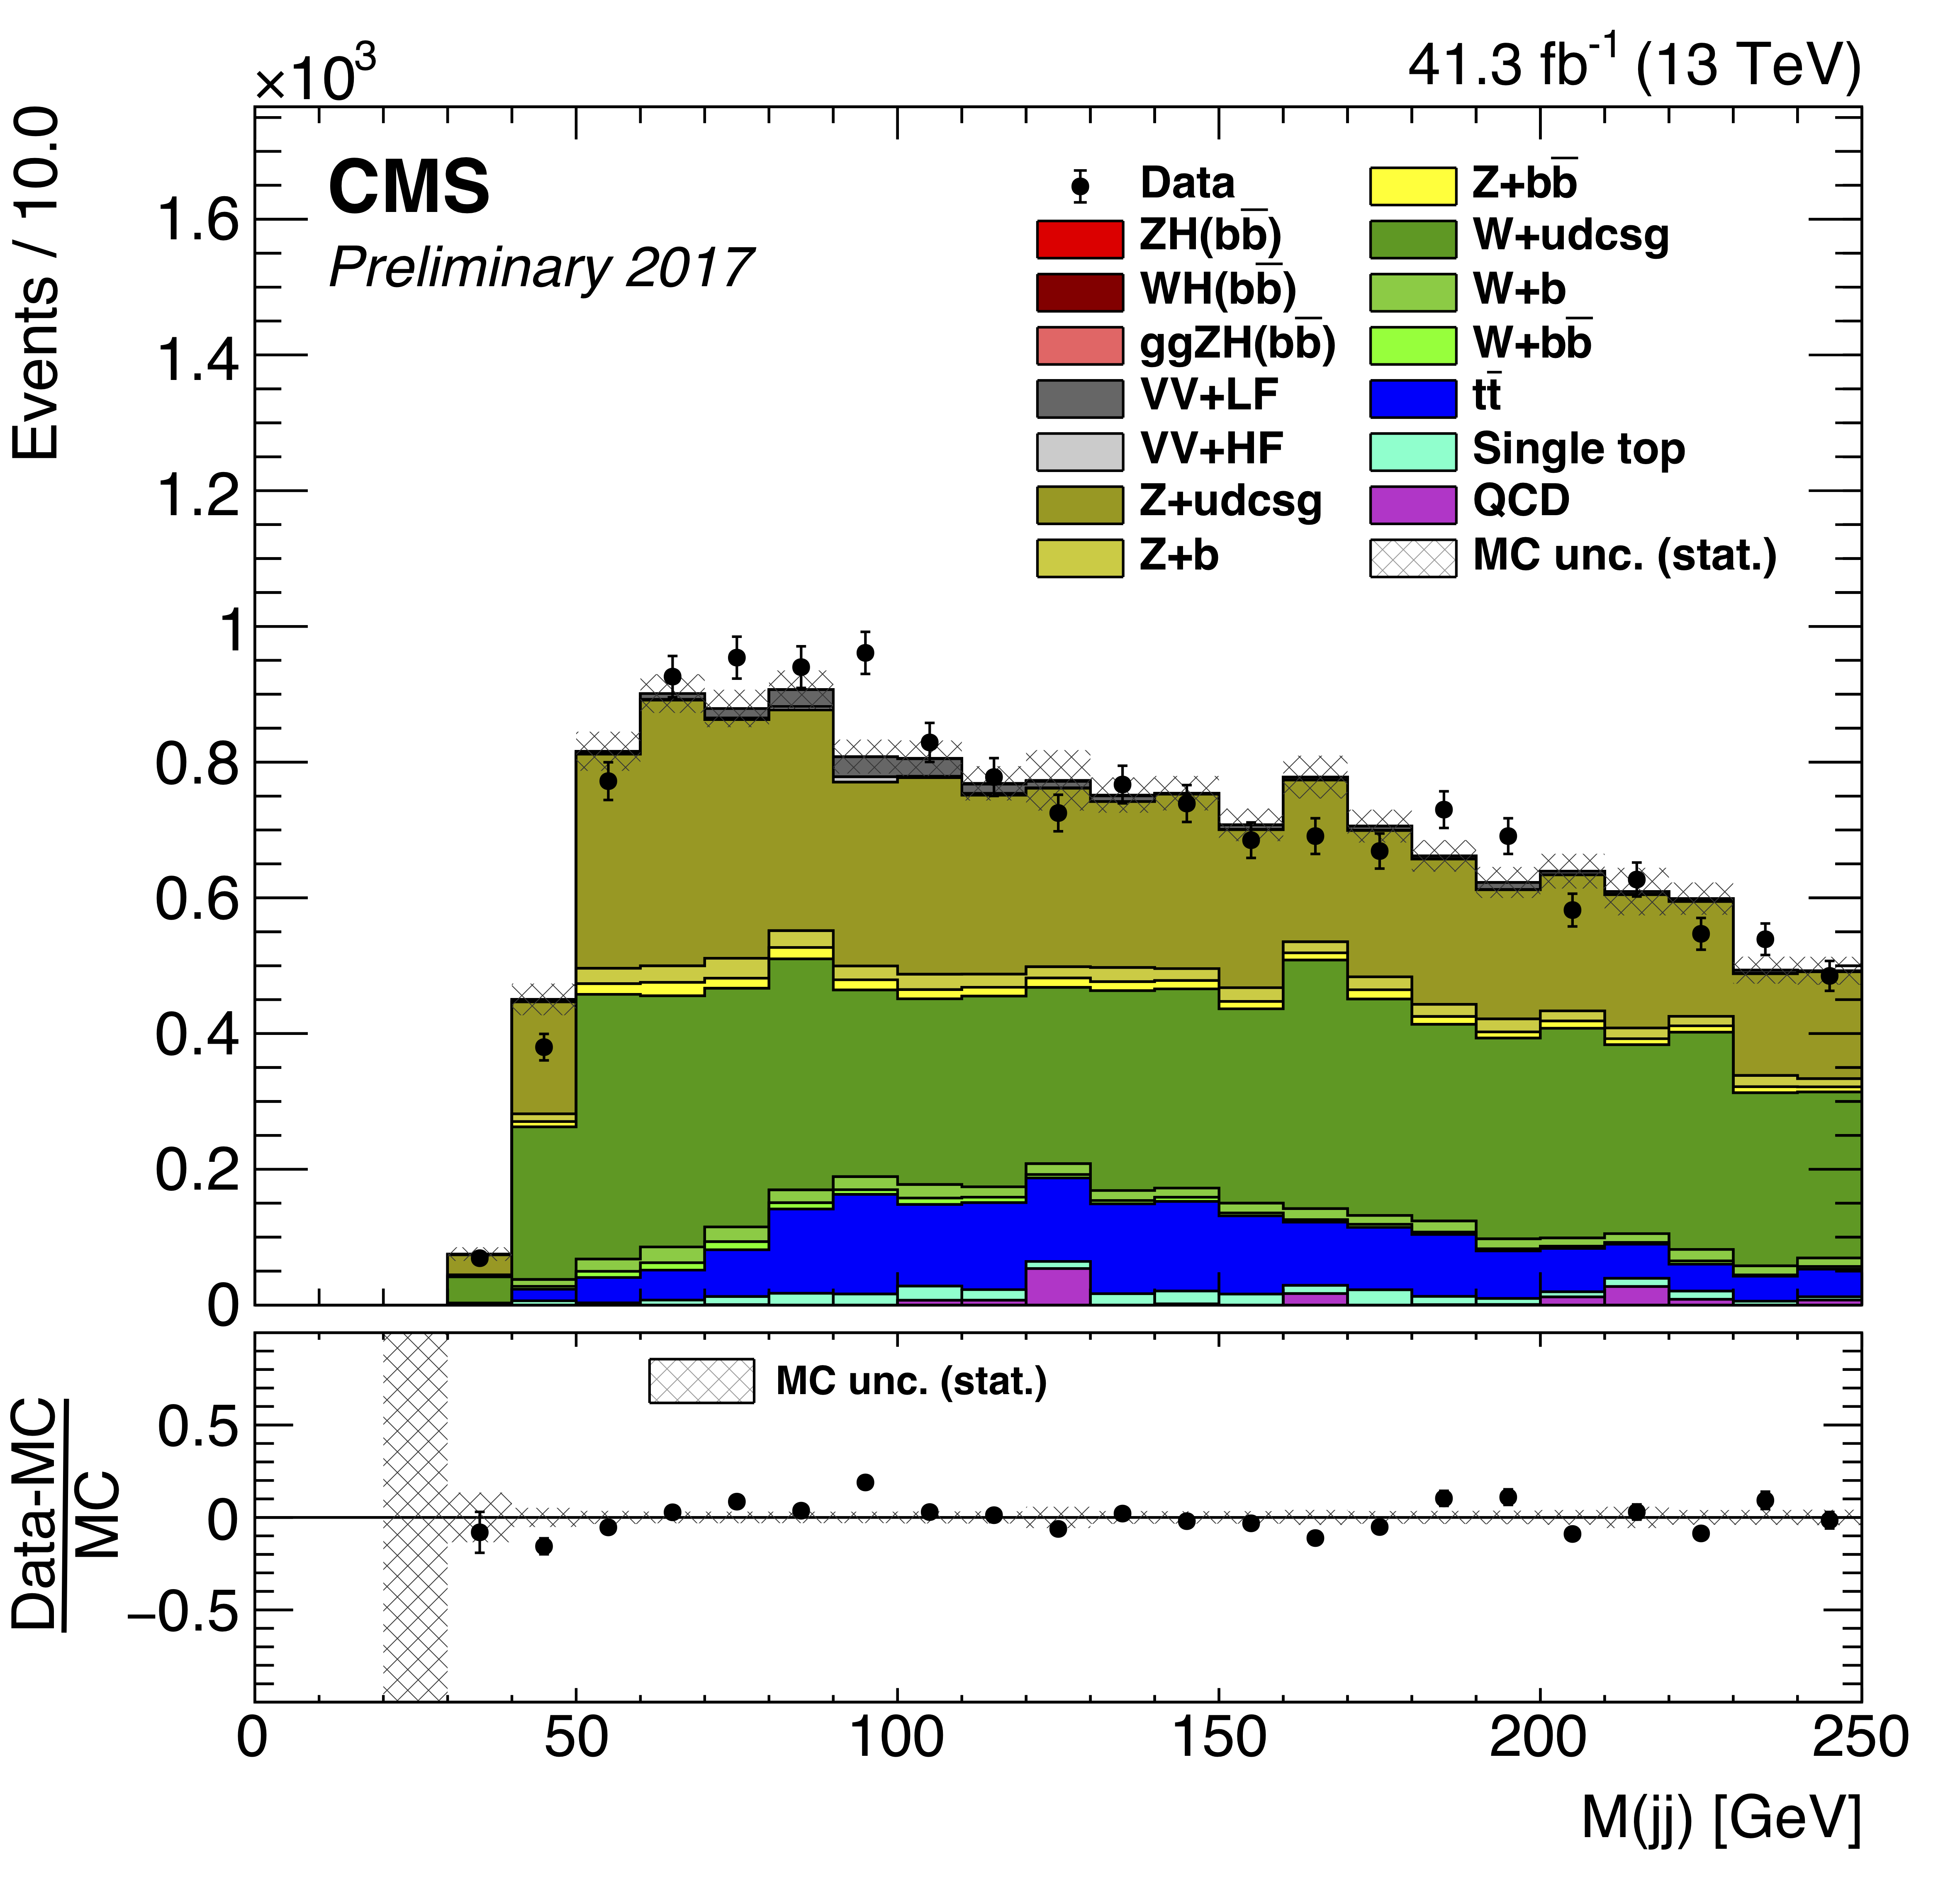
\includegraphics[width=0.39\linewidth]{images/CR_Znn_ZLF/H_mass}}
    \subfigure [] {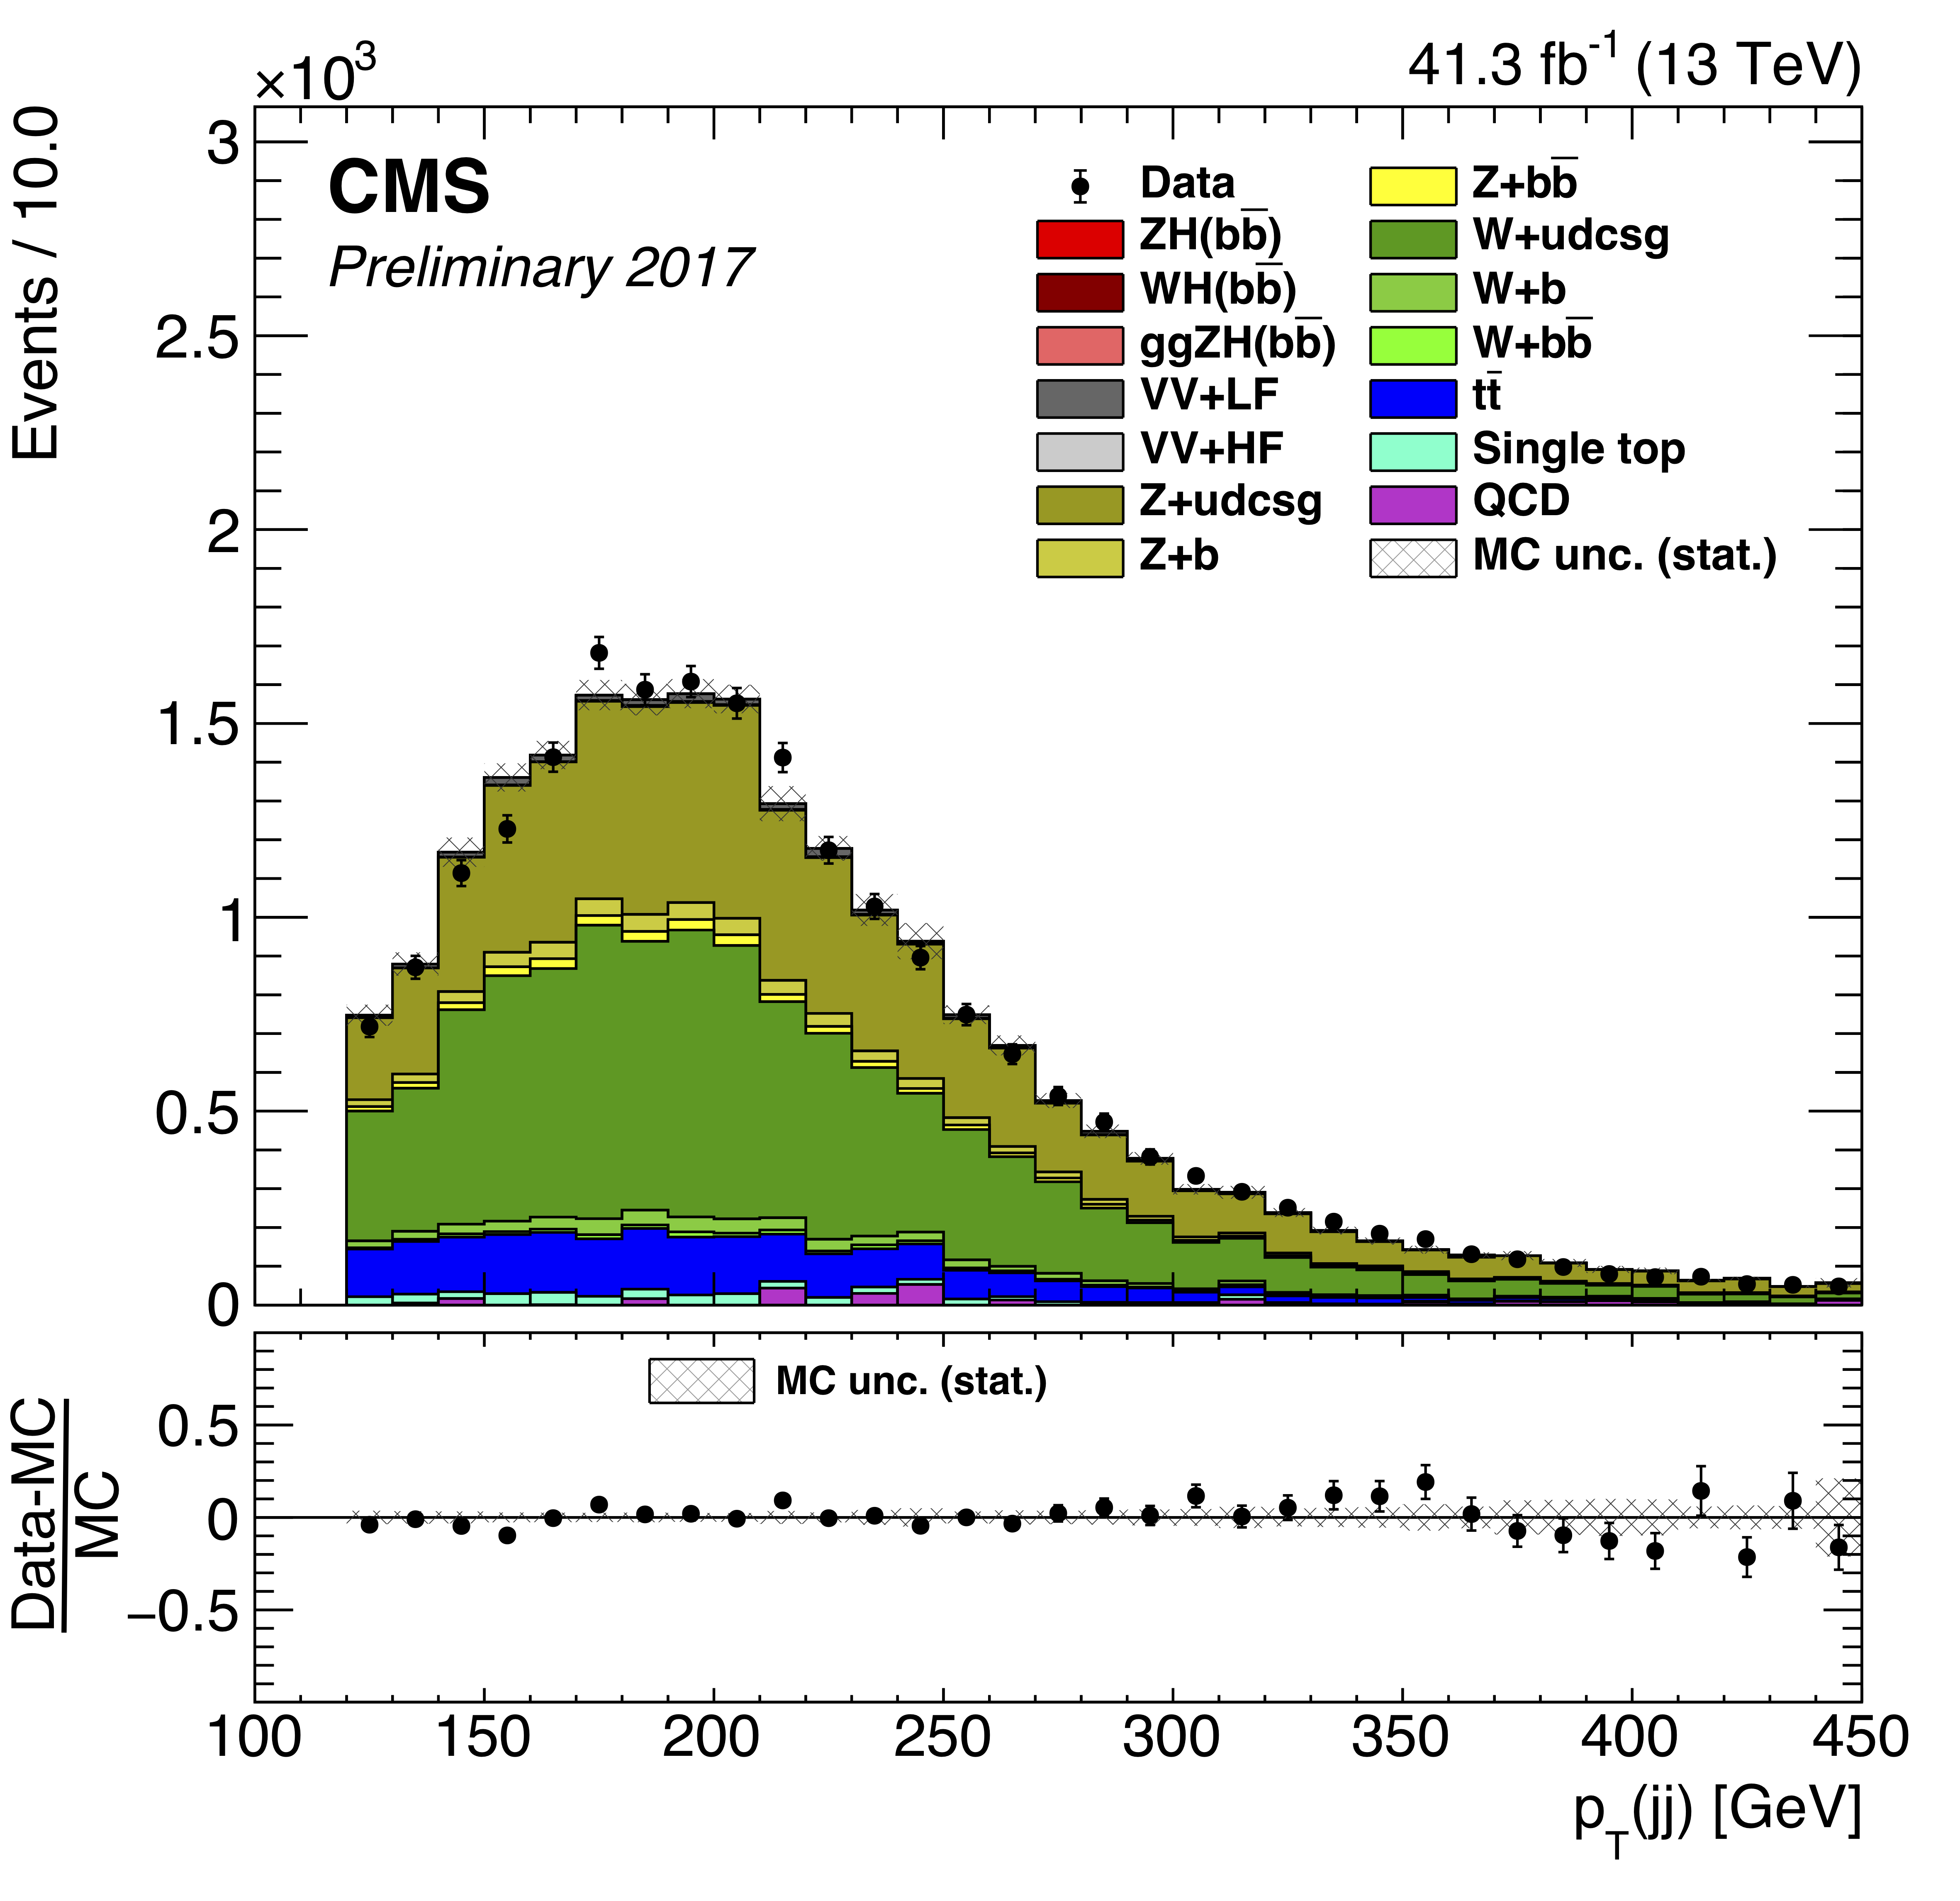
\includegraphics[width=0.39\linewidth]{images/CR_Znn_ZLF/H_pt}}
  }
  \mbox{
    \subfigure [] {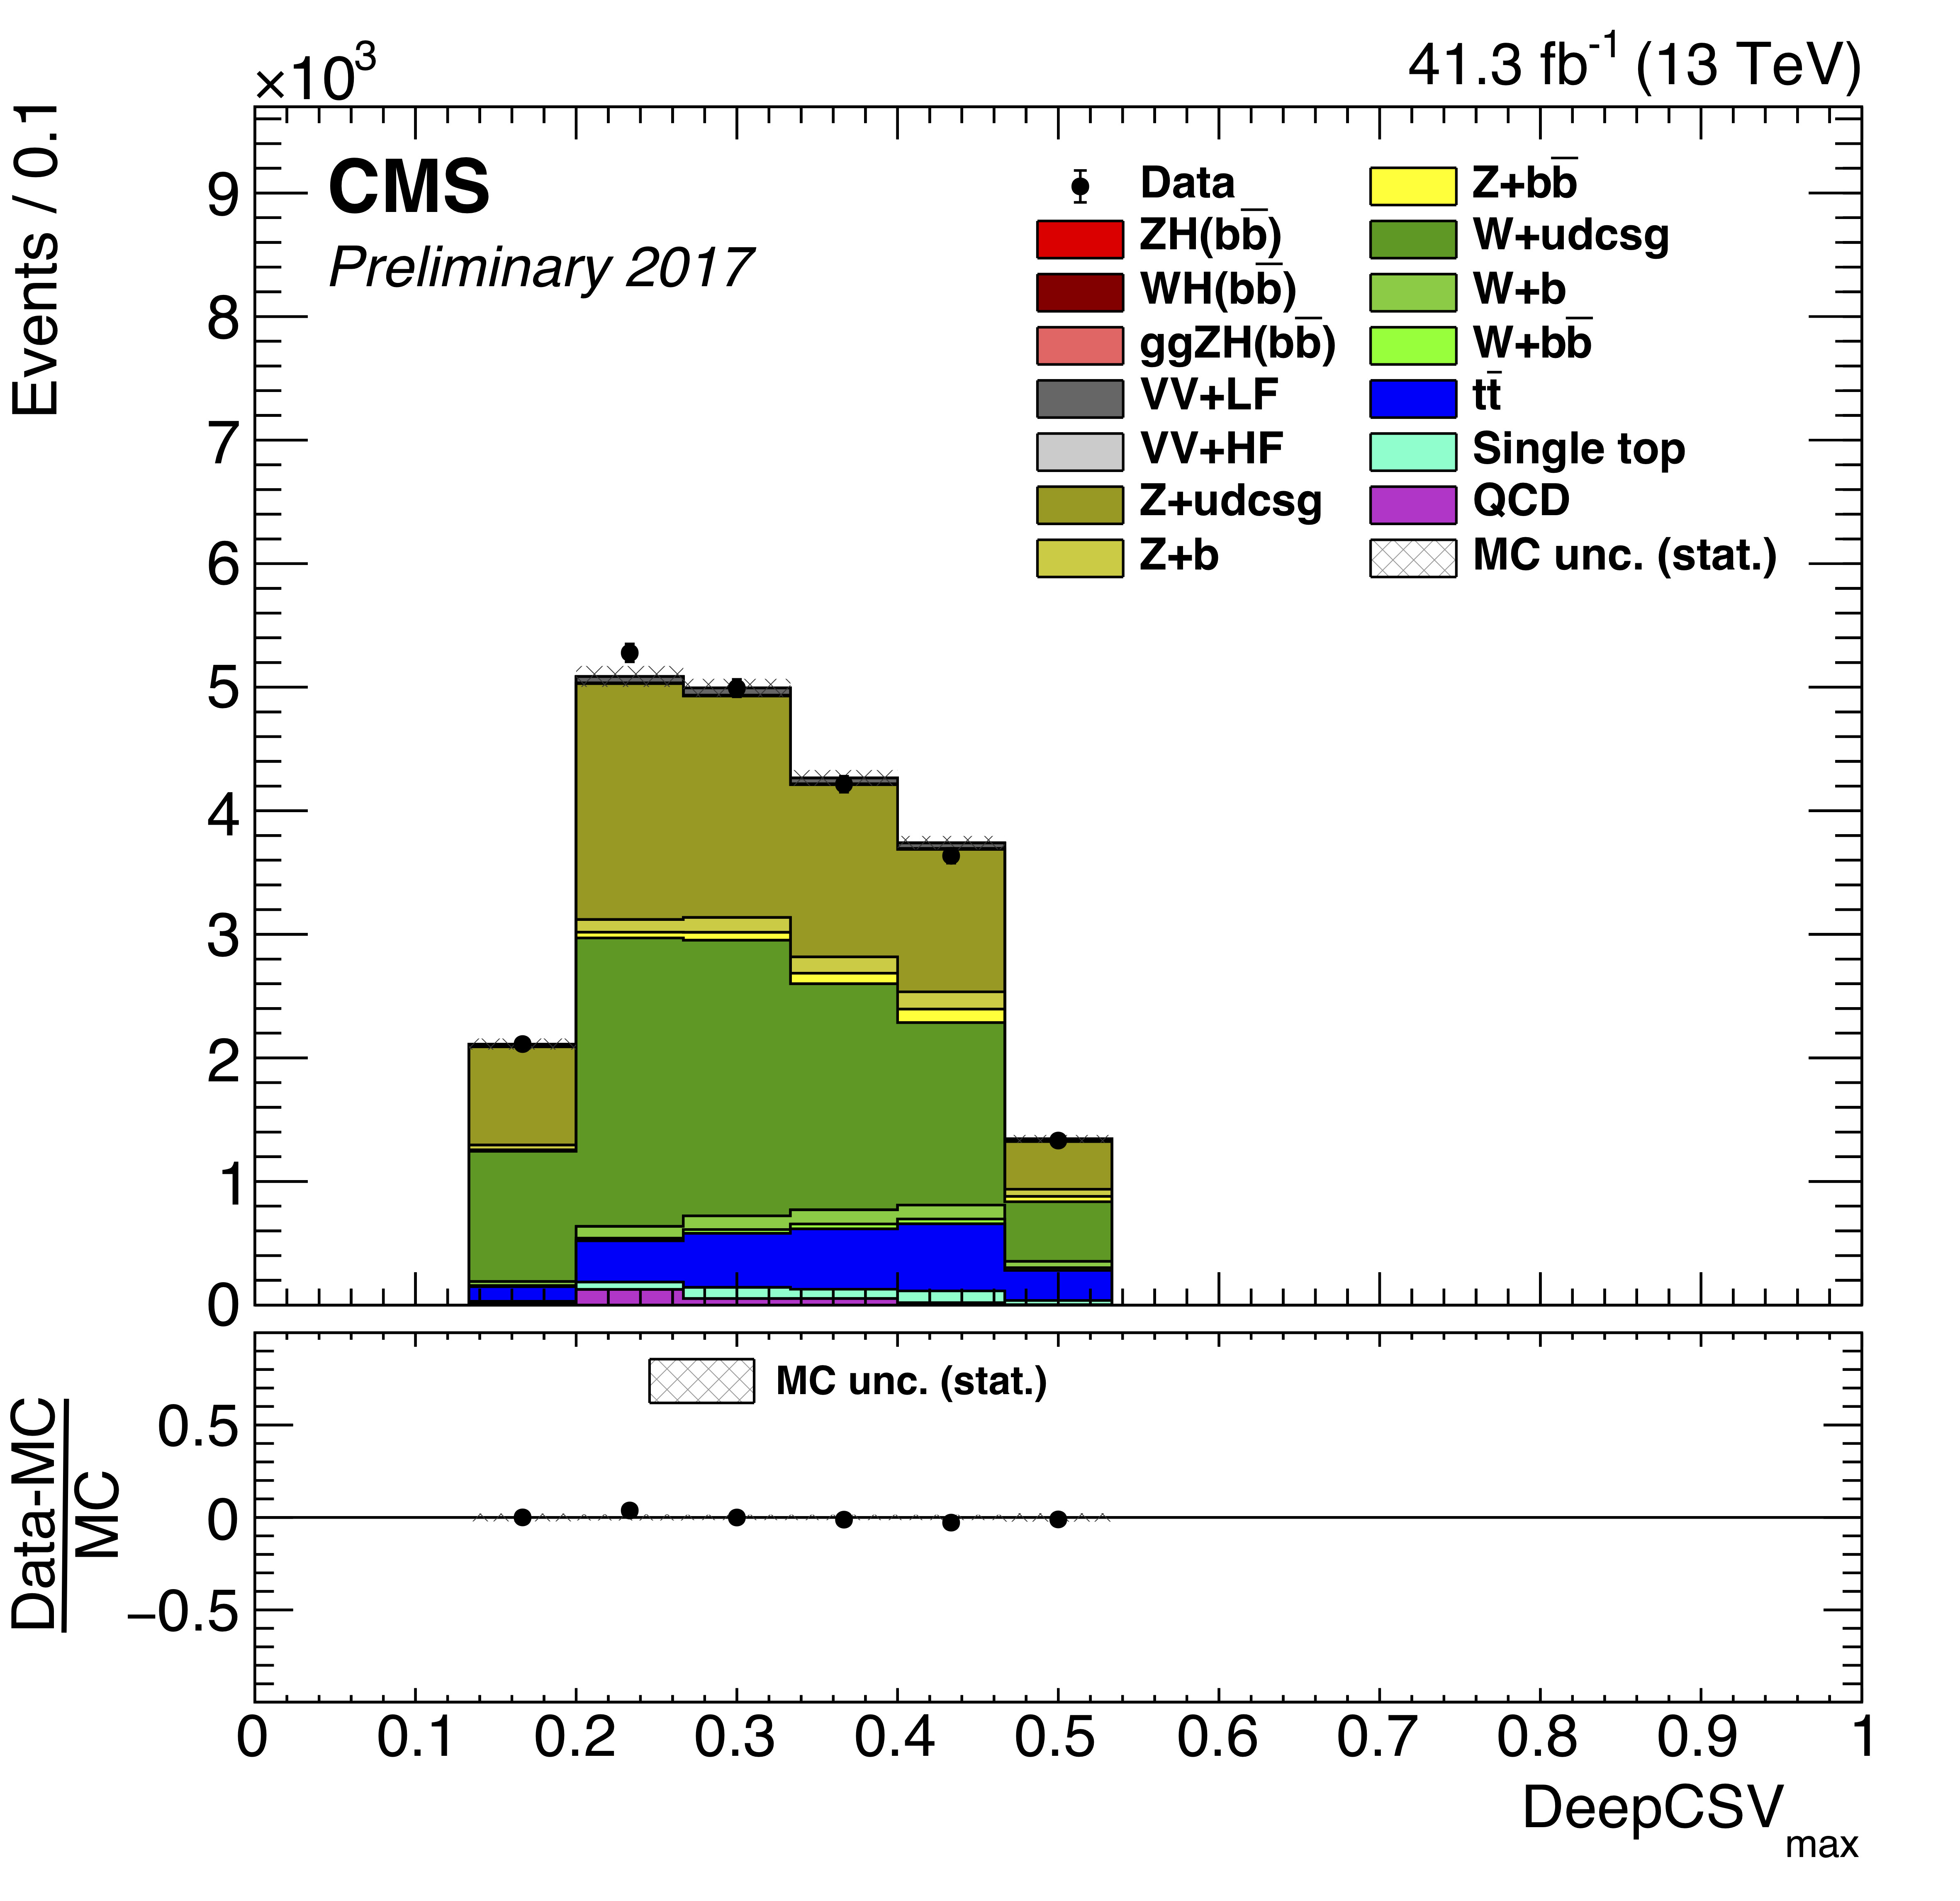
\includegraphics[width=0.39\linewidth]{images/CR_Znn_ZLF/hJets_DeepCSV_0}}
    \subfigure [] {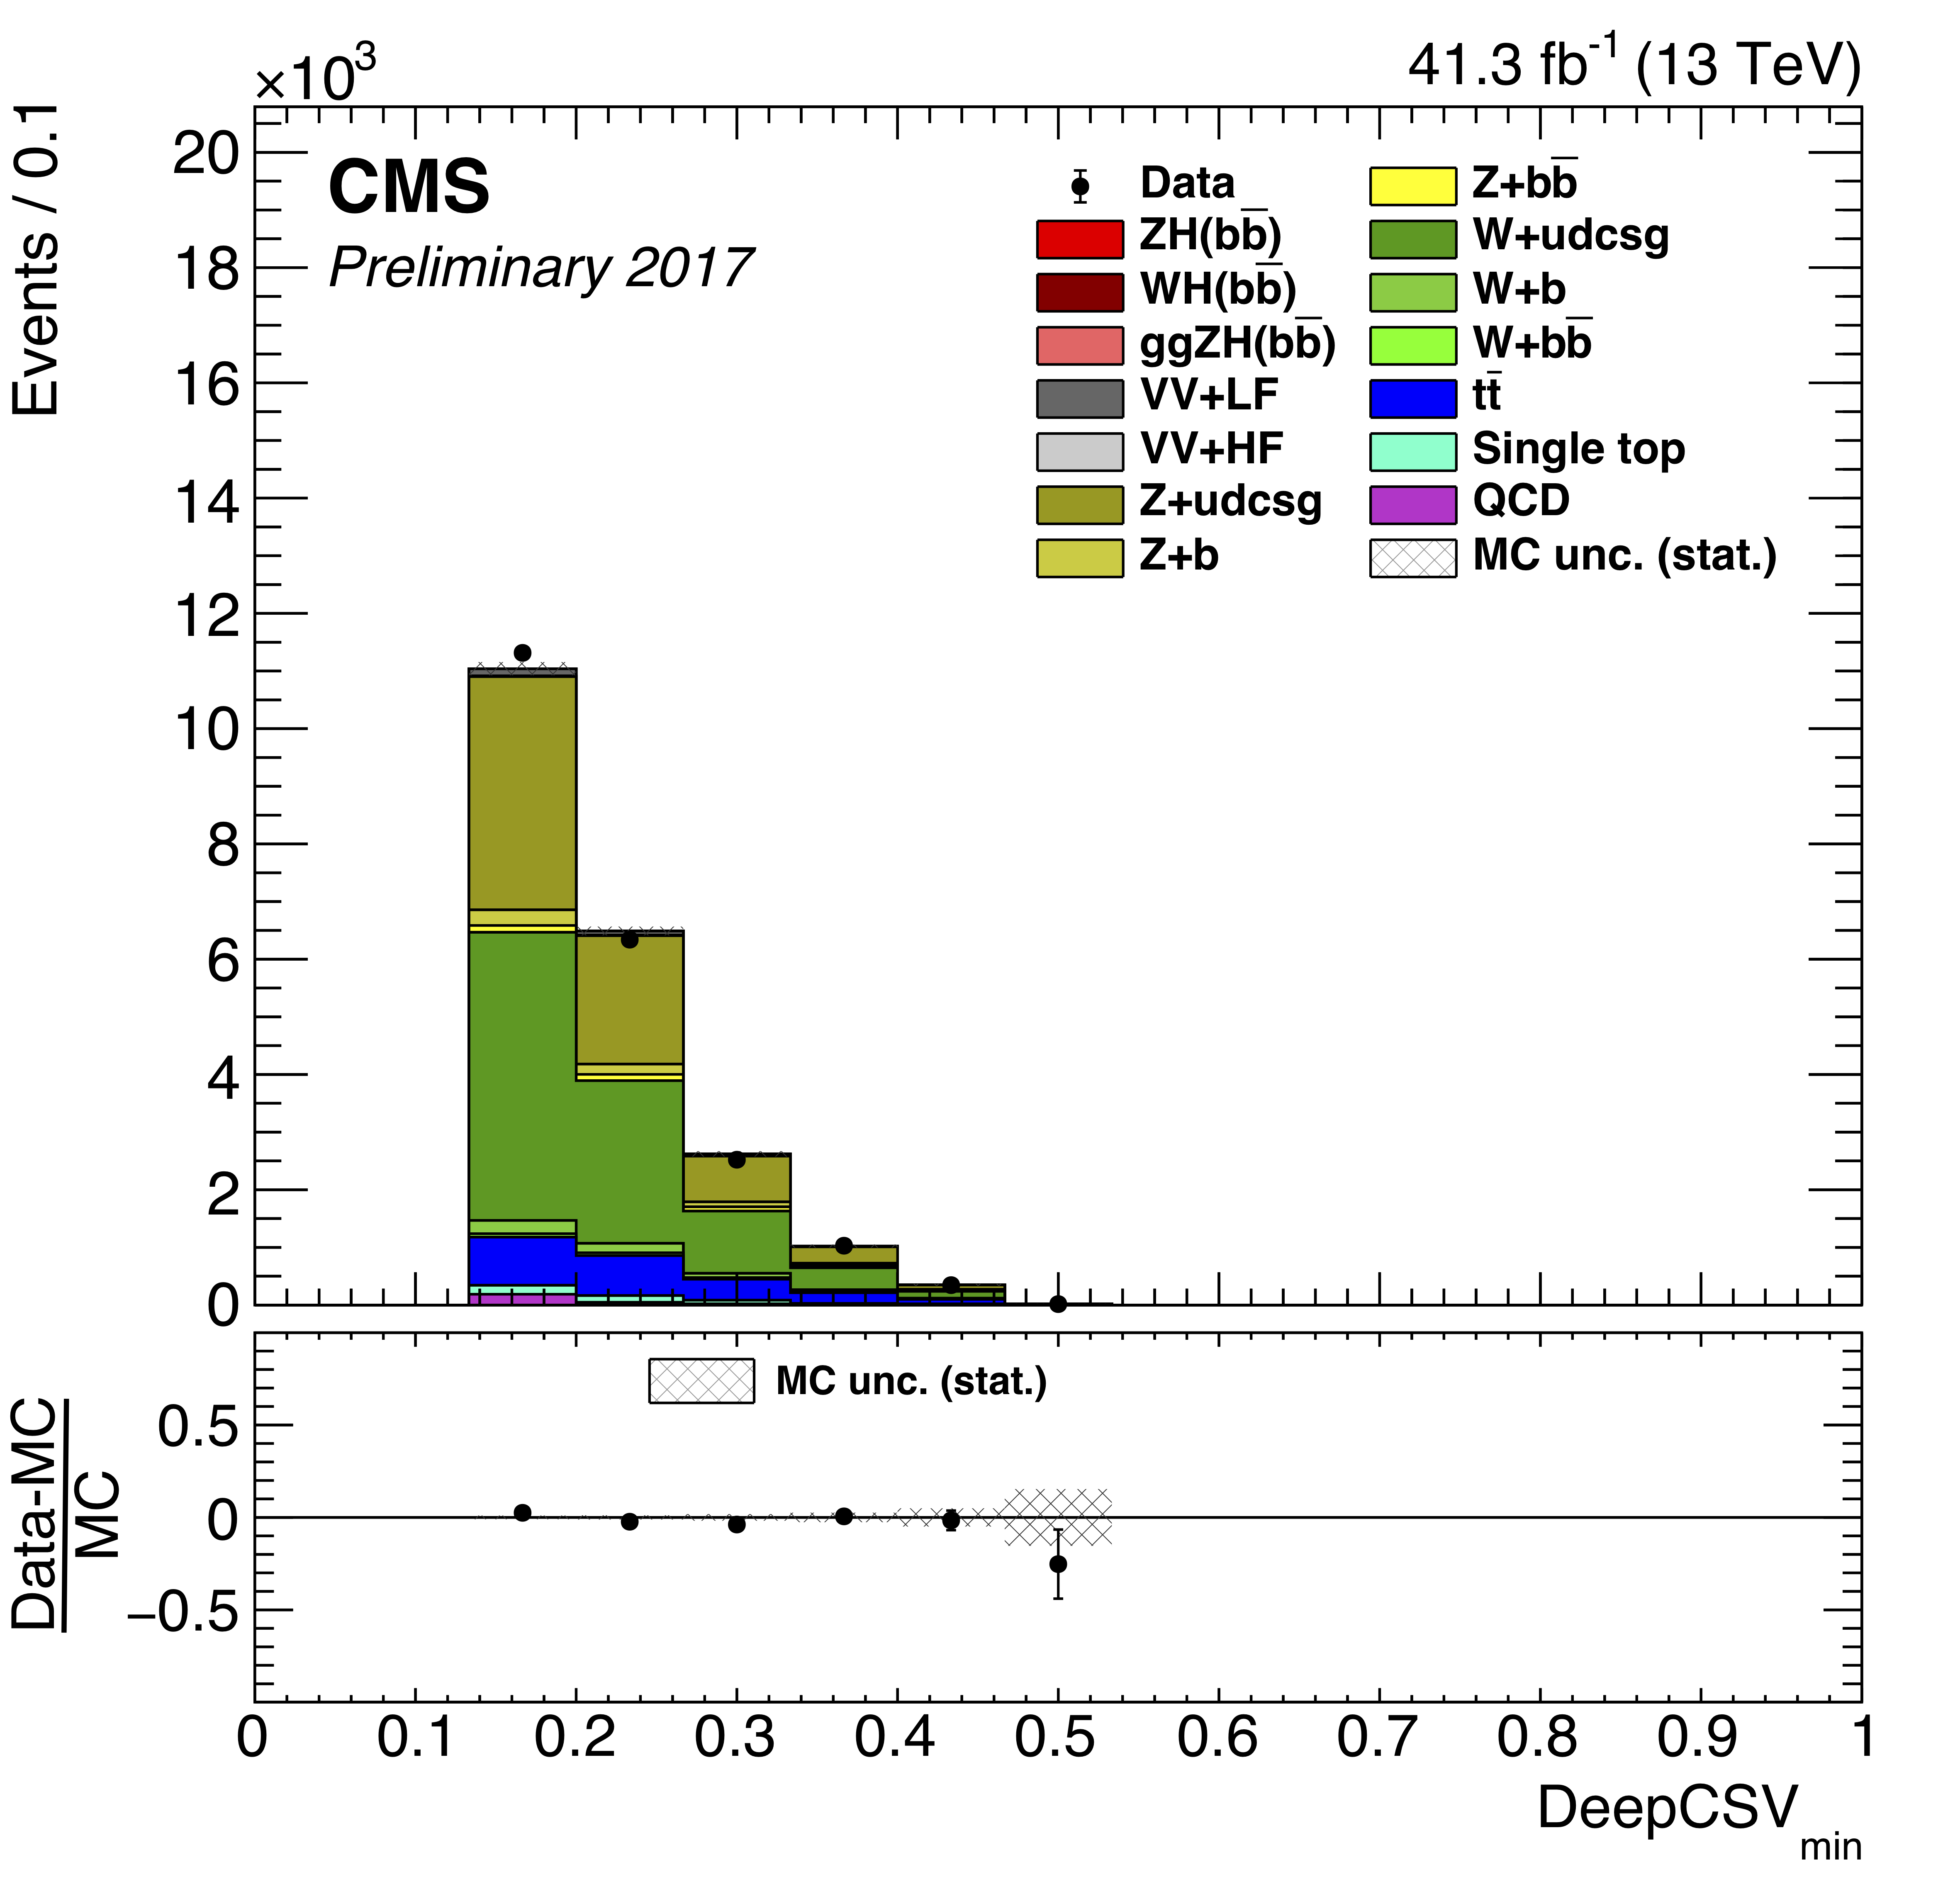
\includegraphics[width=0.39\linewidth]{images/CR_Znn_ZLF/hJets_DeepCSV_1}}
  }
  \mbox{
    \subfigure [] {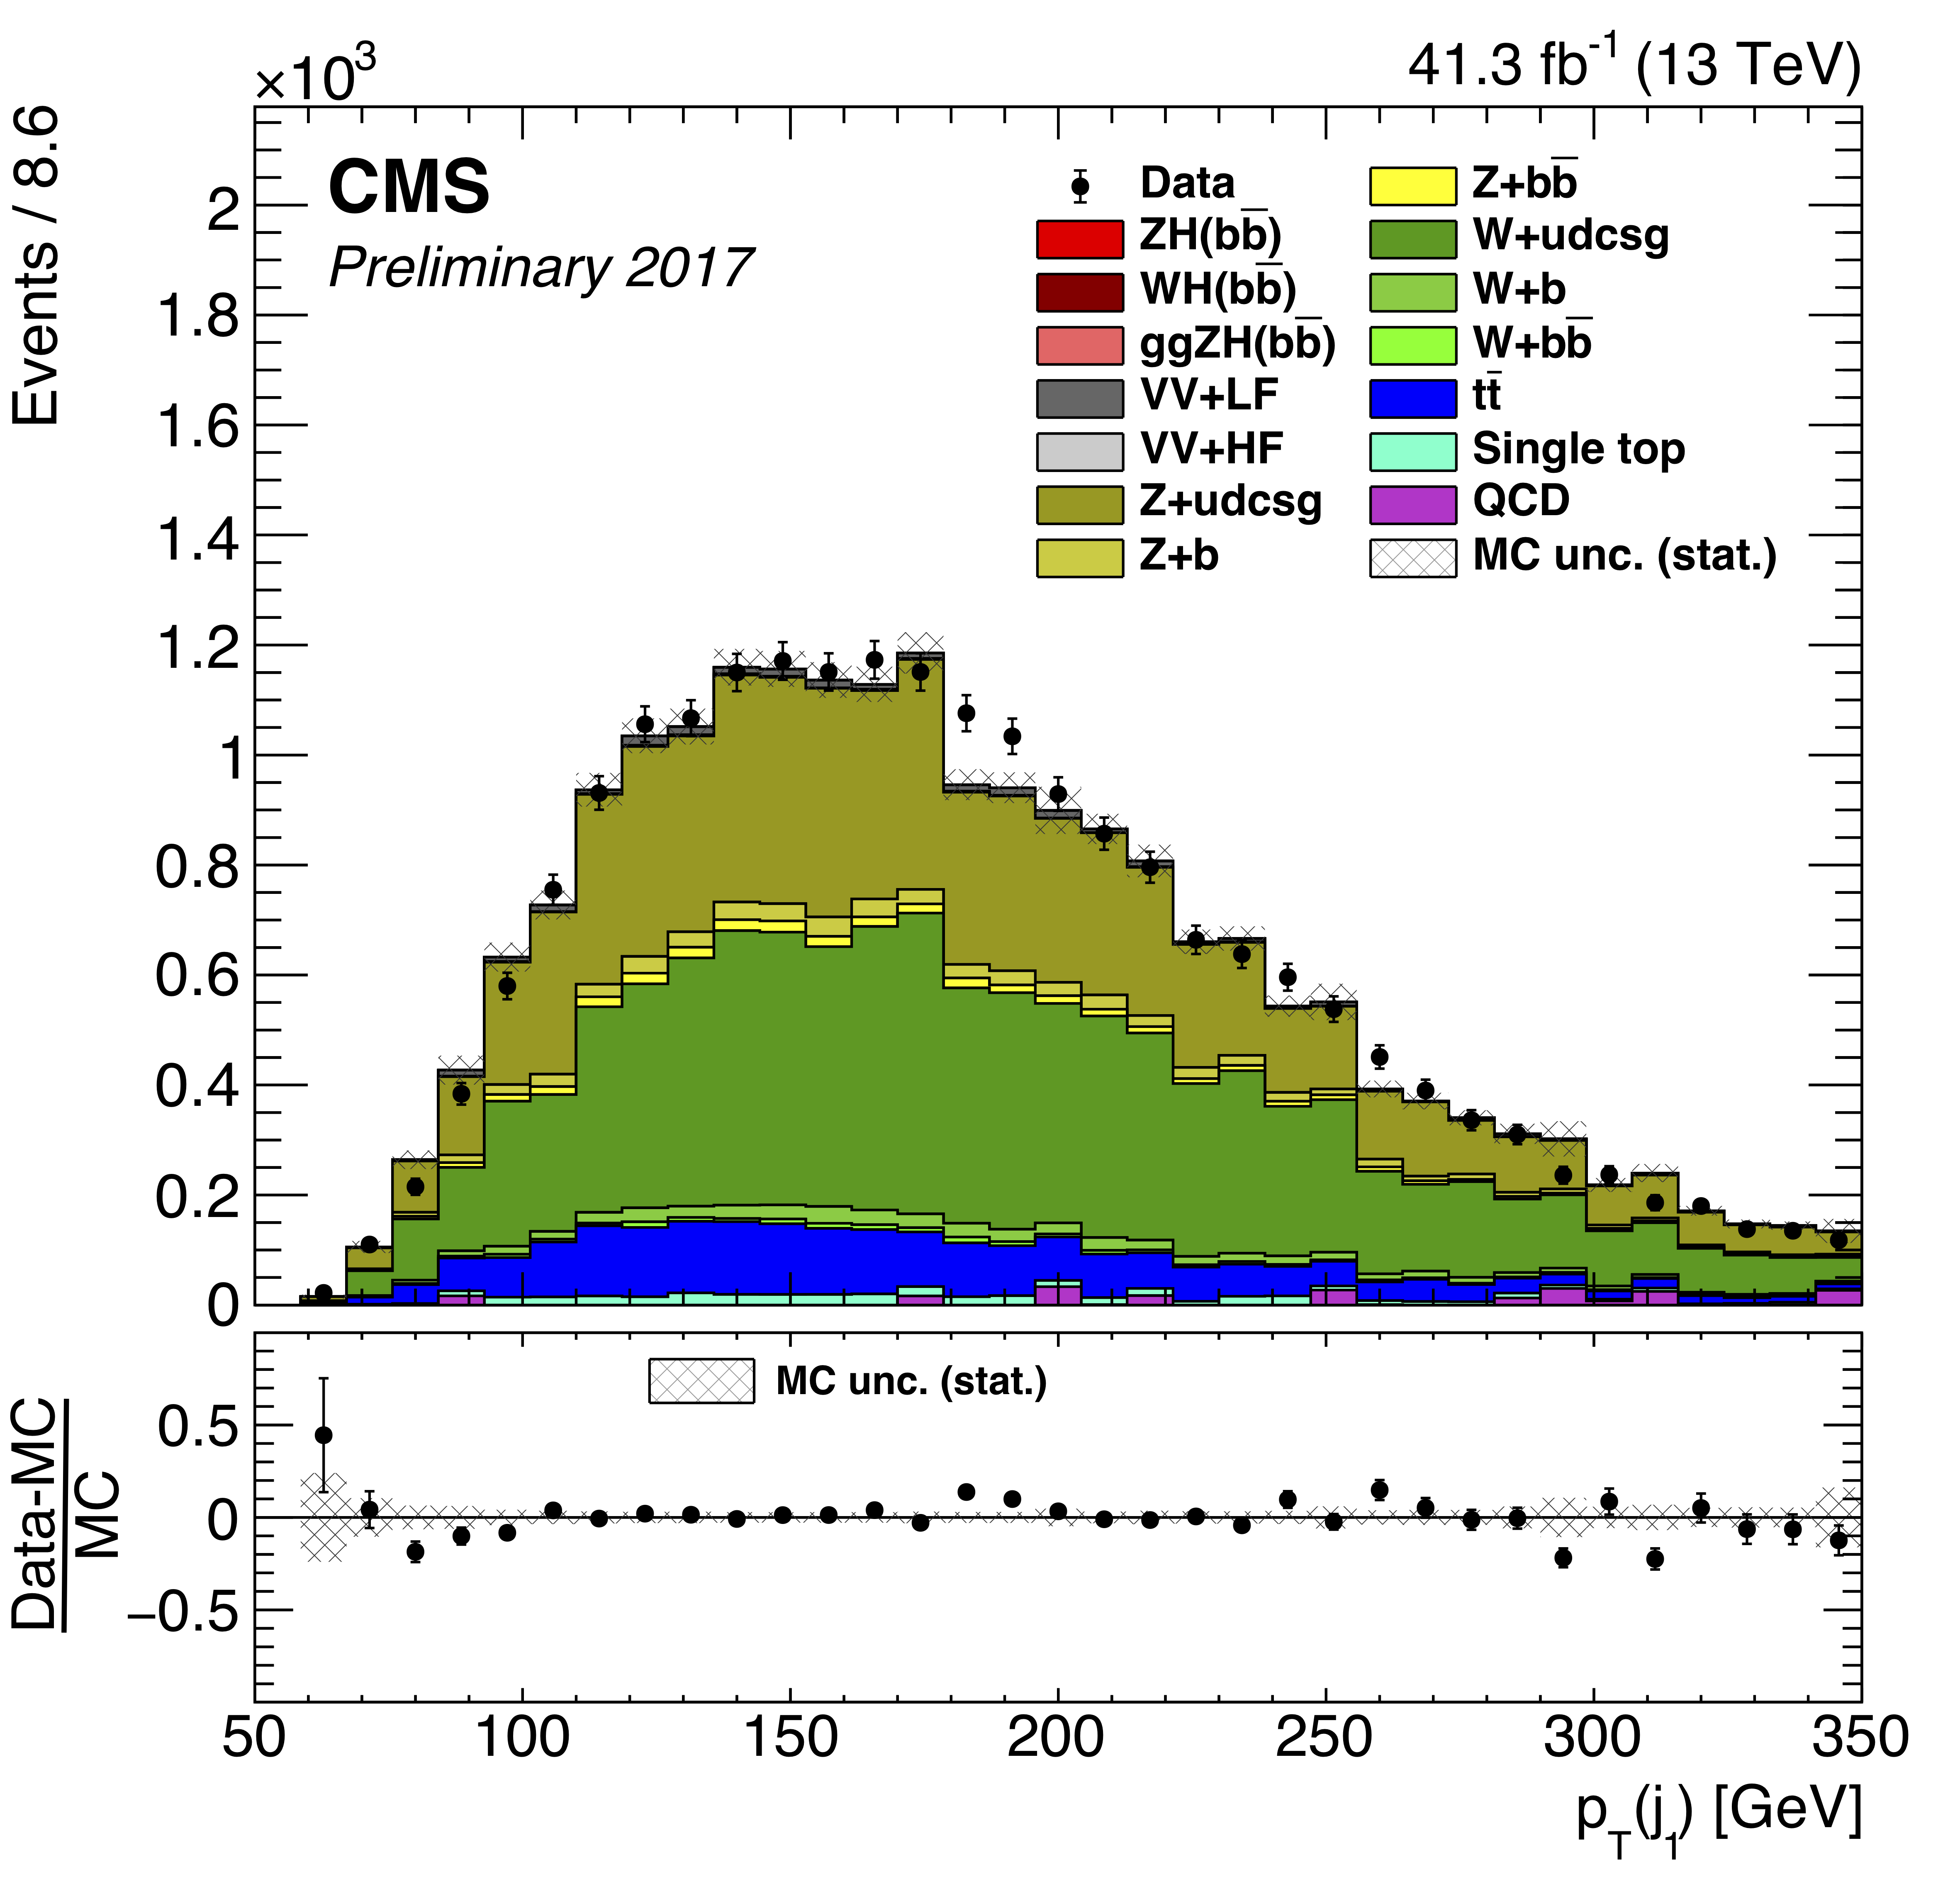
\includegraphics[width=0.39\linewidth]{images/CR_Znn_ZLF/hJets_leadingPt}}
    \subfigure [] {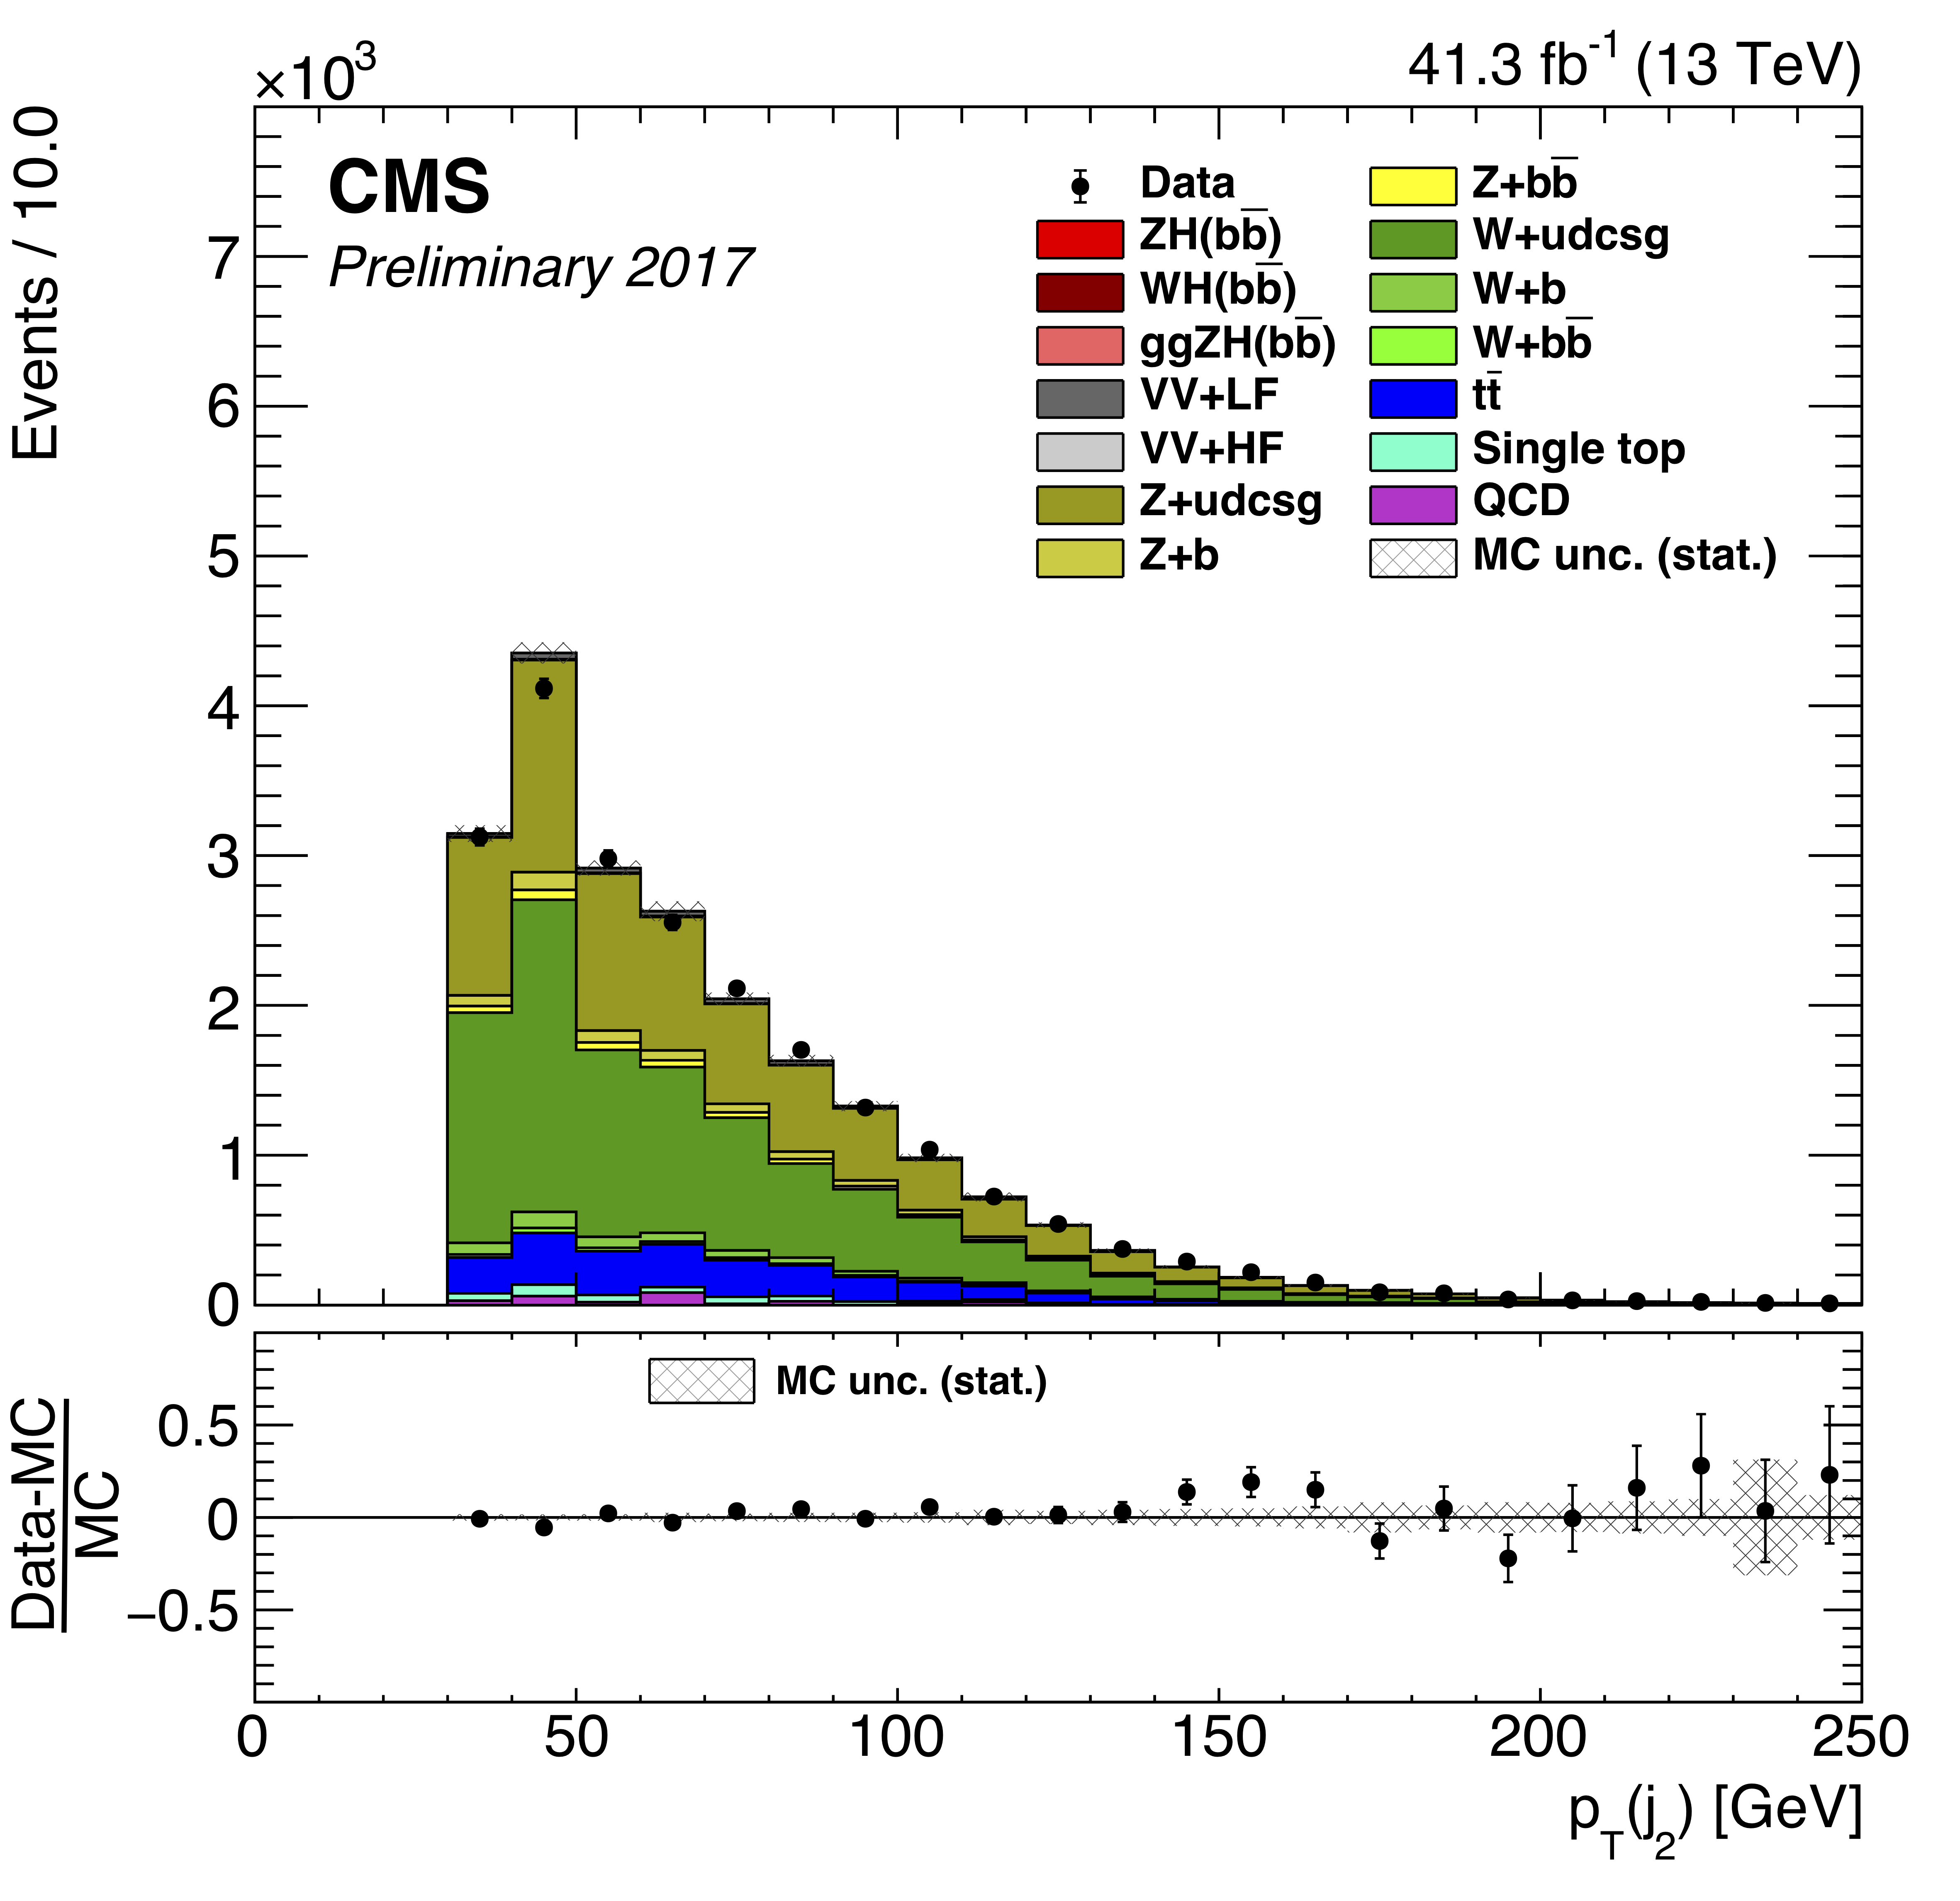
\includegraphics[width=0.39\linewidth]{images/CR_Znn_ZLF/hJets_subleadingPt}}
  }
  \caption[\bosZ+light Control Region Distributions for the \ZnnH\ Channel]{The distributions of variables in the \bosZ+light control region of the \ZnnH\ channel: A) $m(jj)$, B) $\pT(jj)$, C) \btagmax, D) \btagmin, E) \pTjmax, F) \pTjmin.}
  \label{fig:CR_Znn_ZLF_1}
\end{figure}

\clearpage

\begin{figure}[htbp]
  \centering
  \mbox{
    \subfigure [] {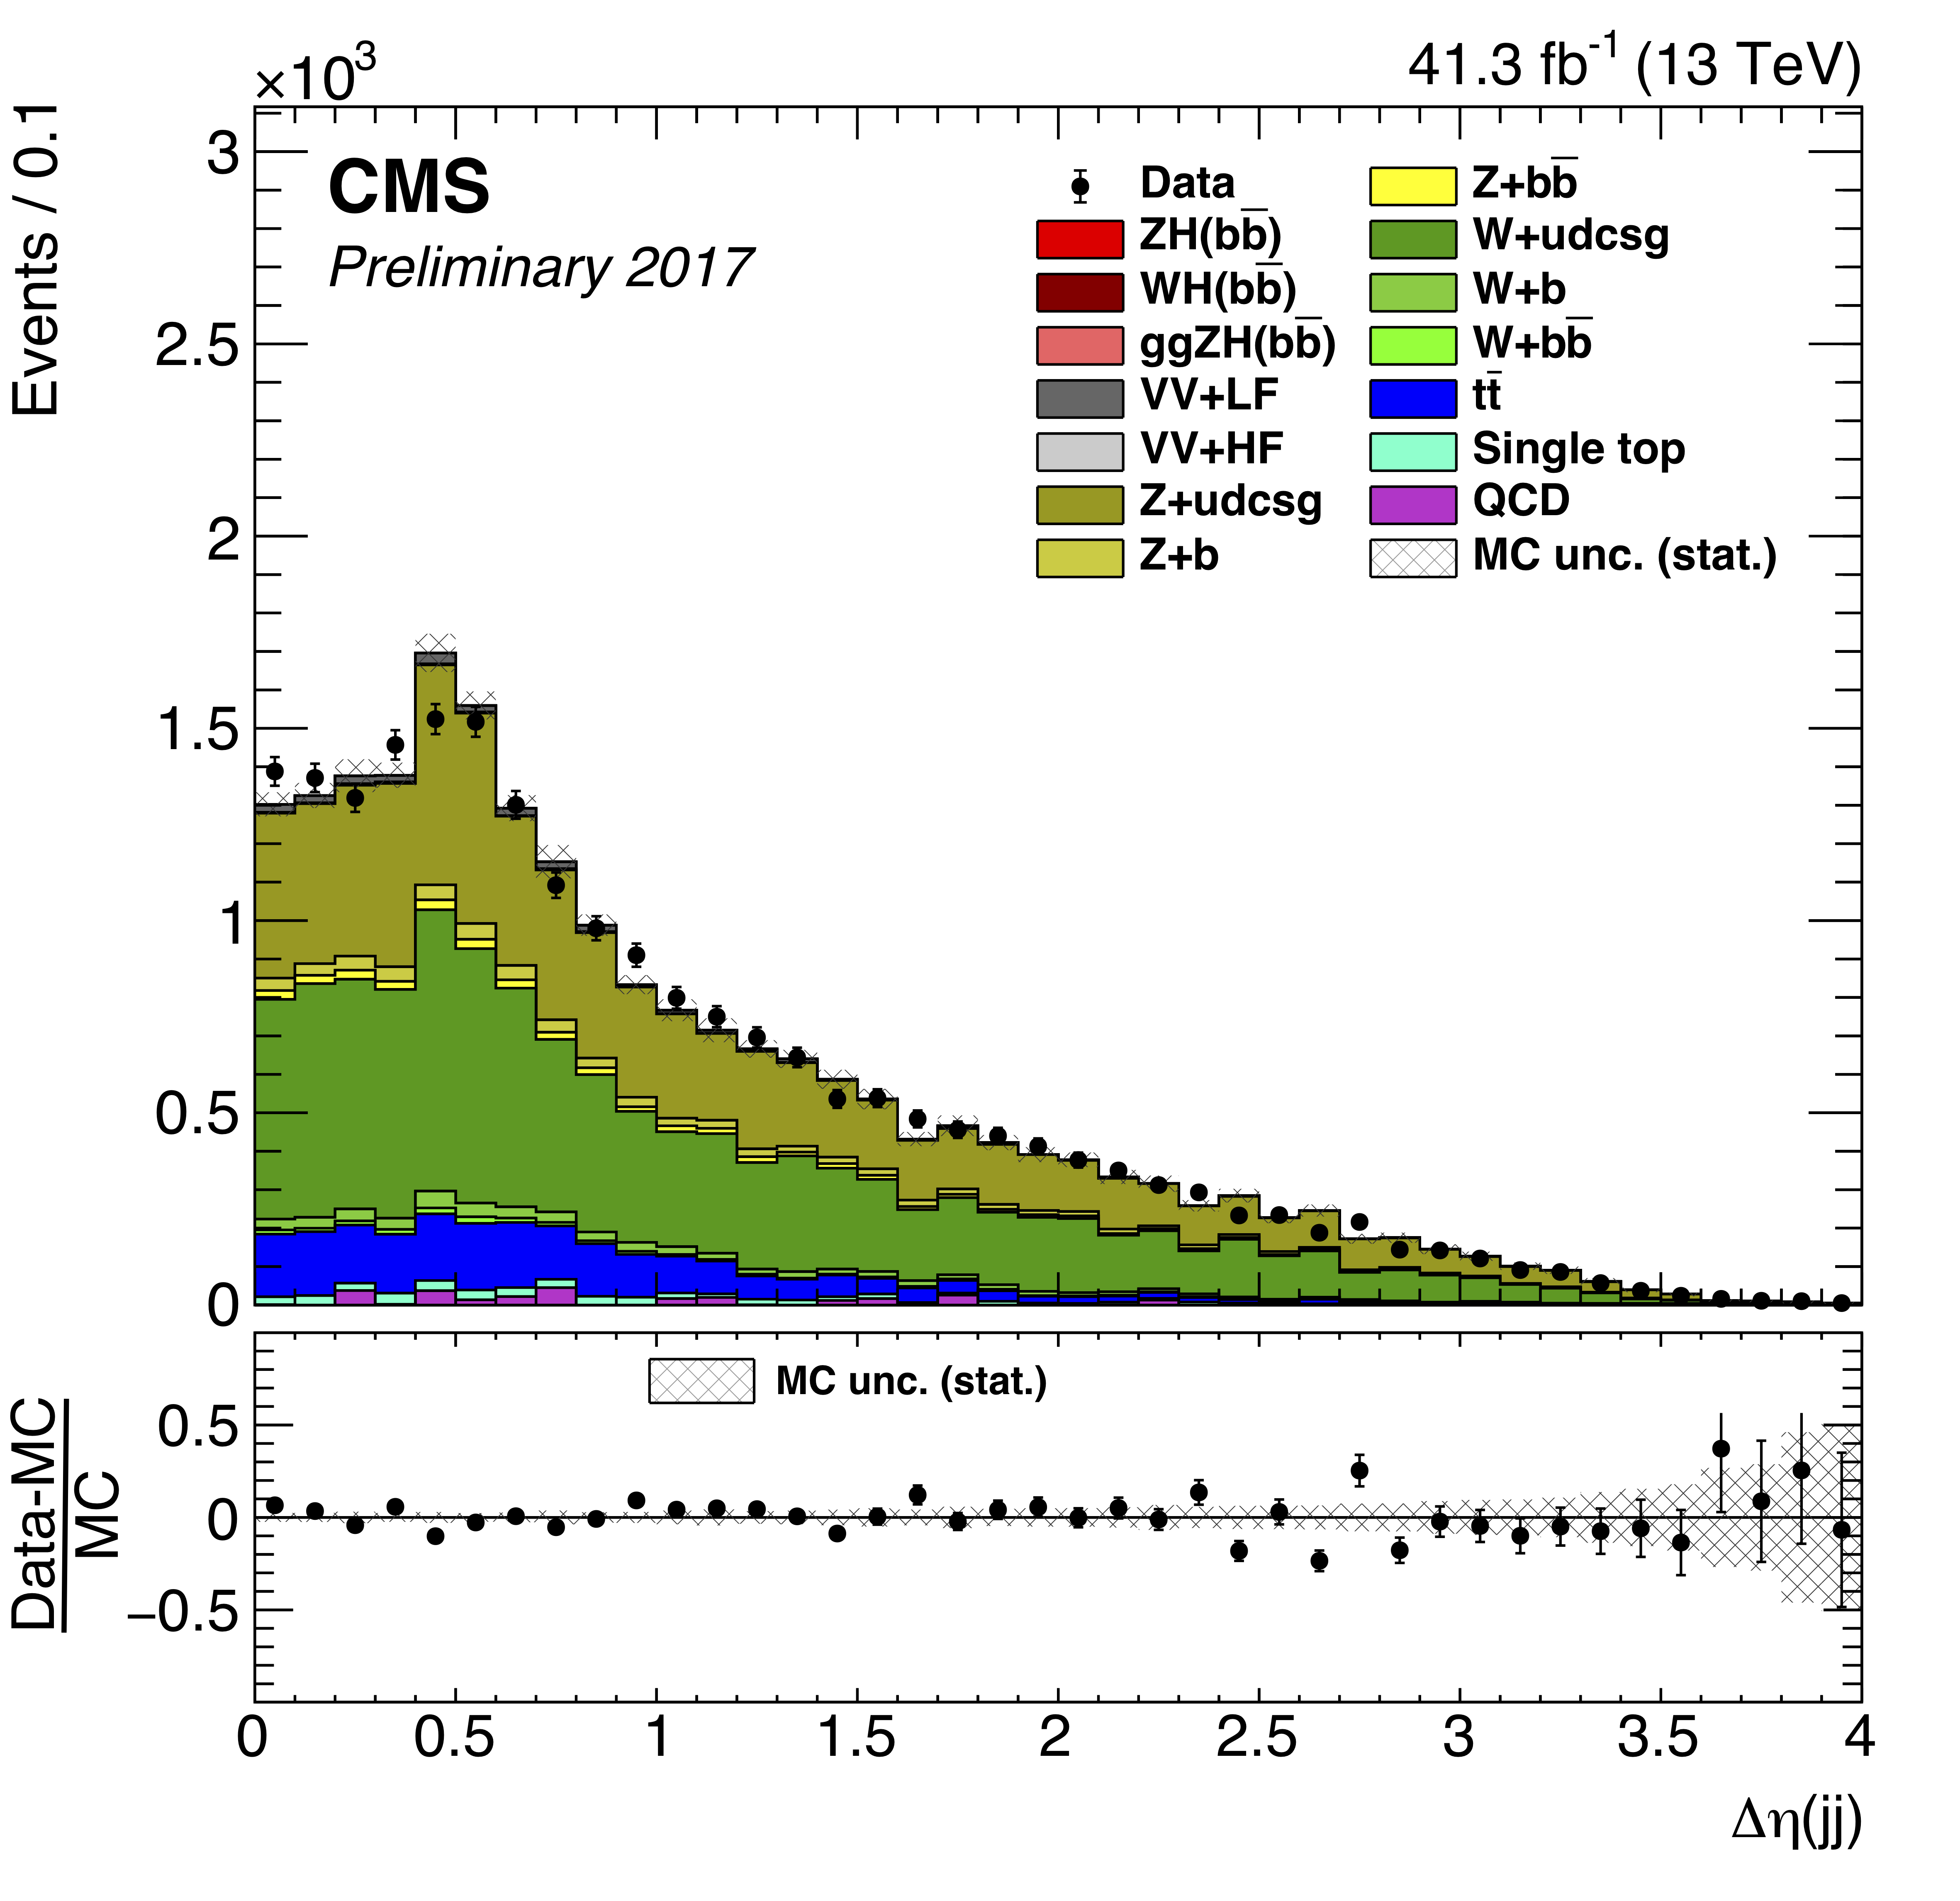
\includegraphics[width=0.39\linewidth]{images/CR_Znn_ZLF/HJ1_HJ2_dEta}}
    \subfigure [] {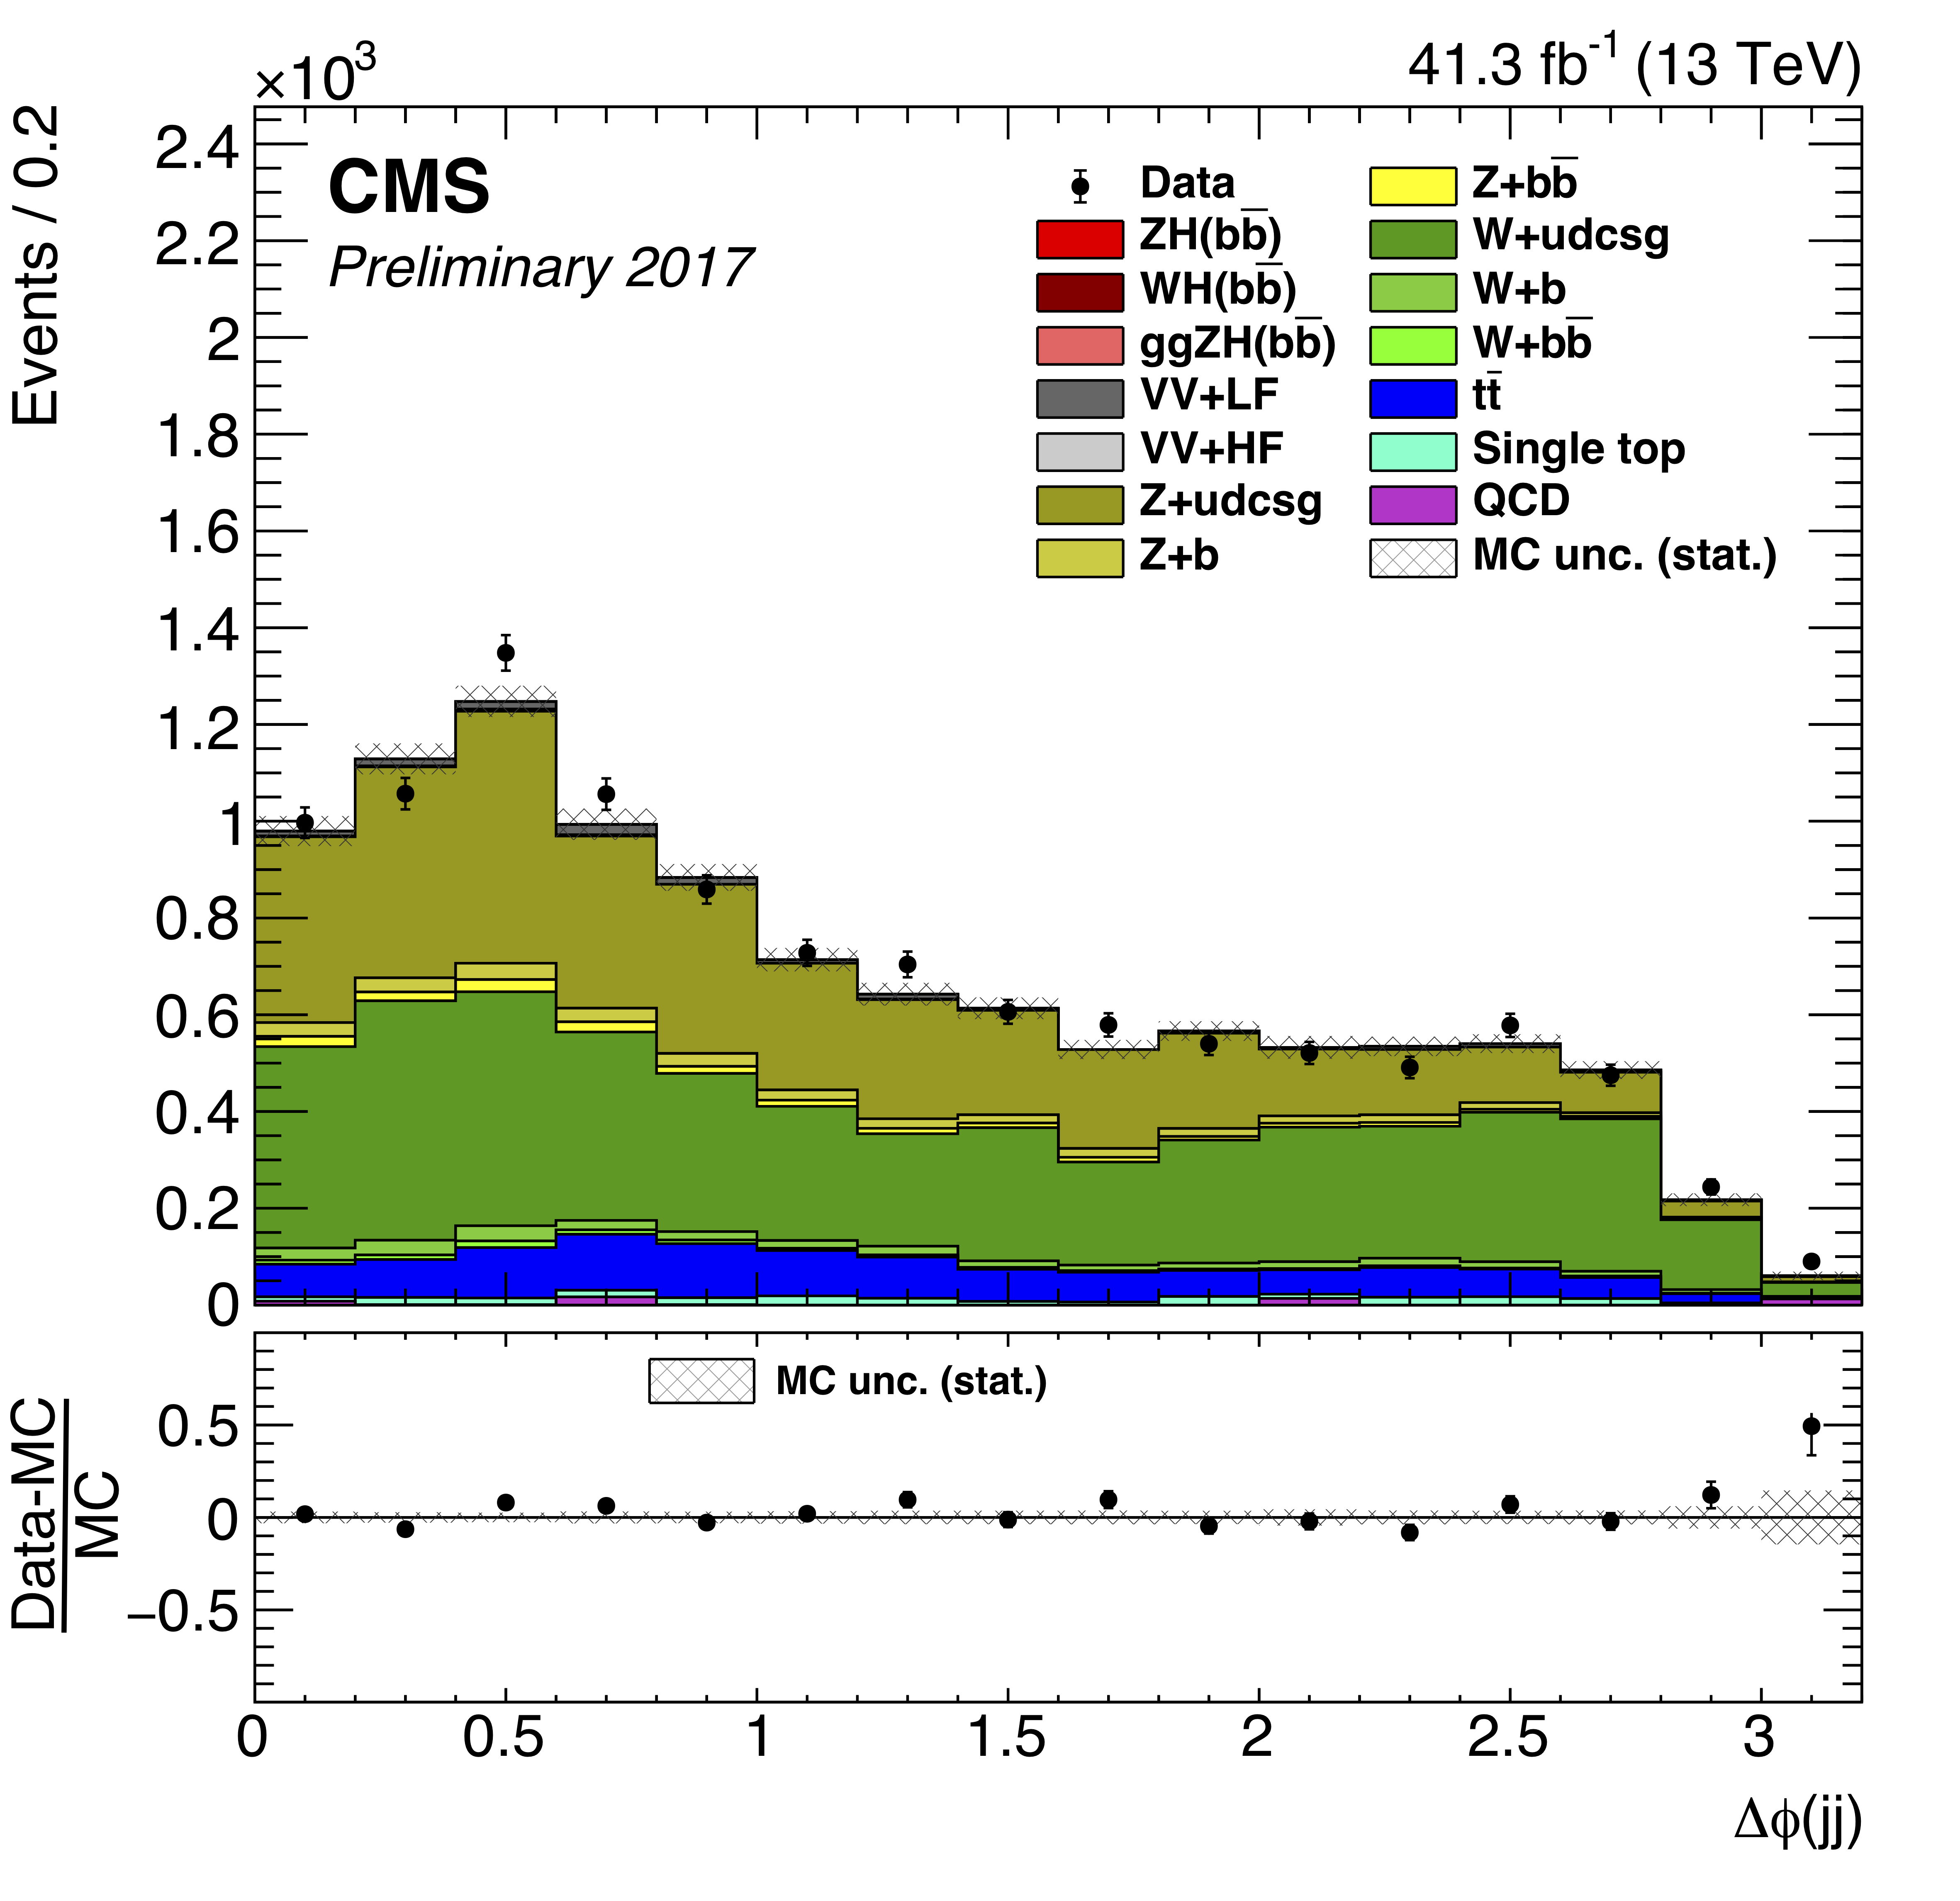
\includegraphics[width=0.39\linewidth]{images/CR_Znn_ZLF/HJ1_HJ2_dPhi}}
  }
  \mbox{
    \subfigure [] {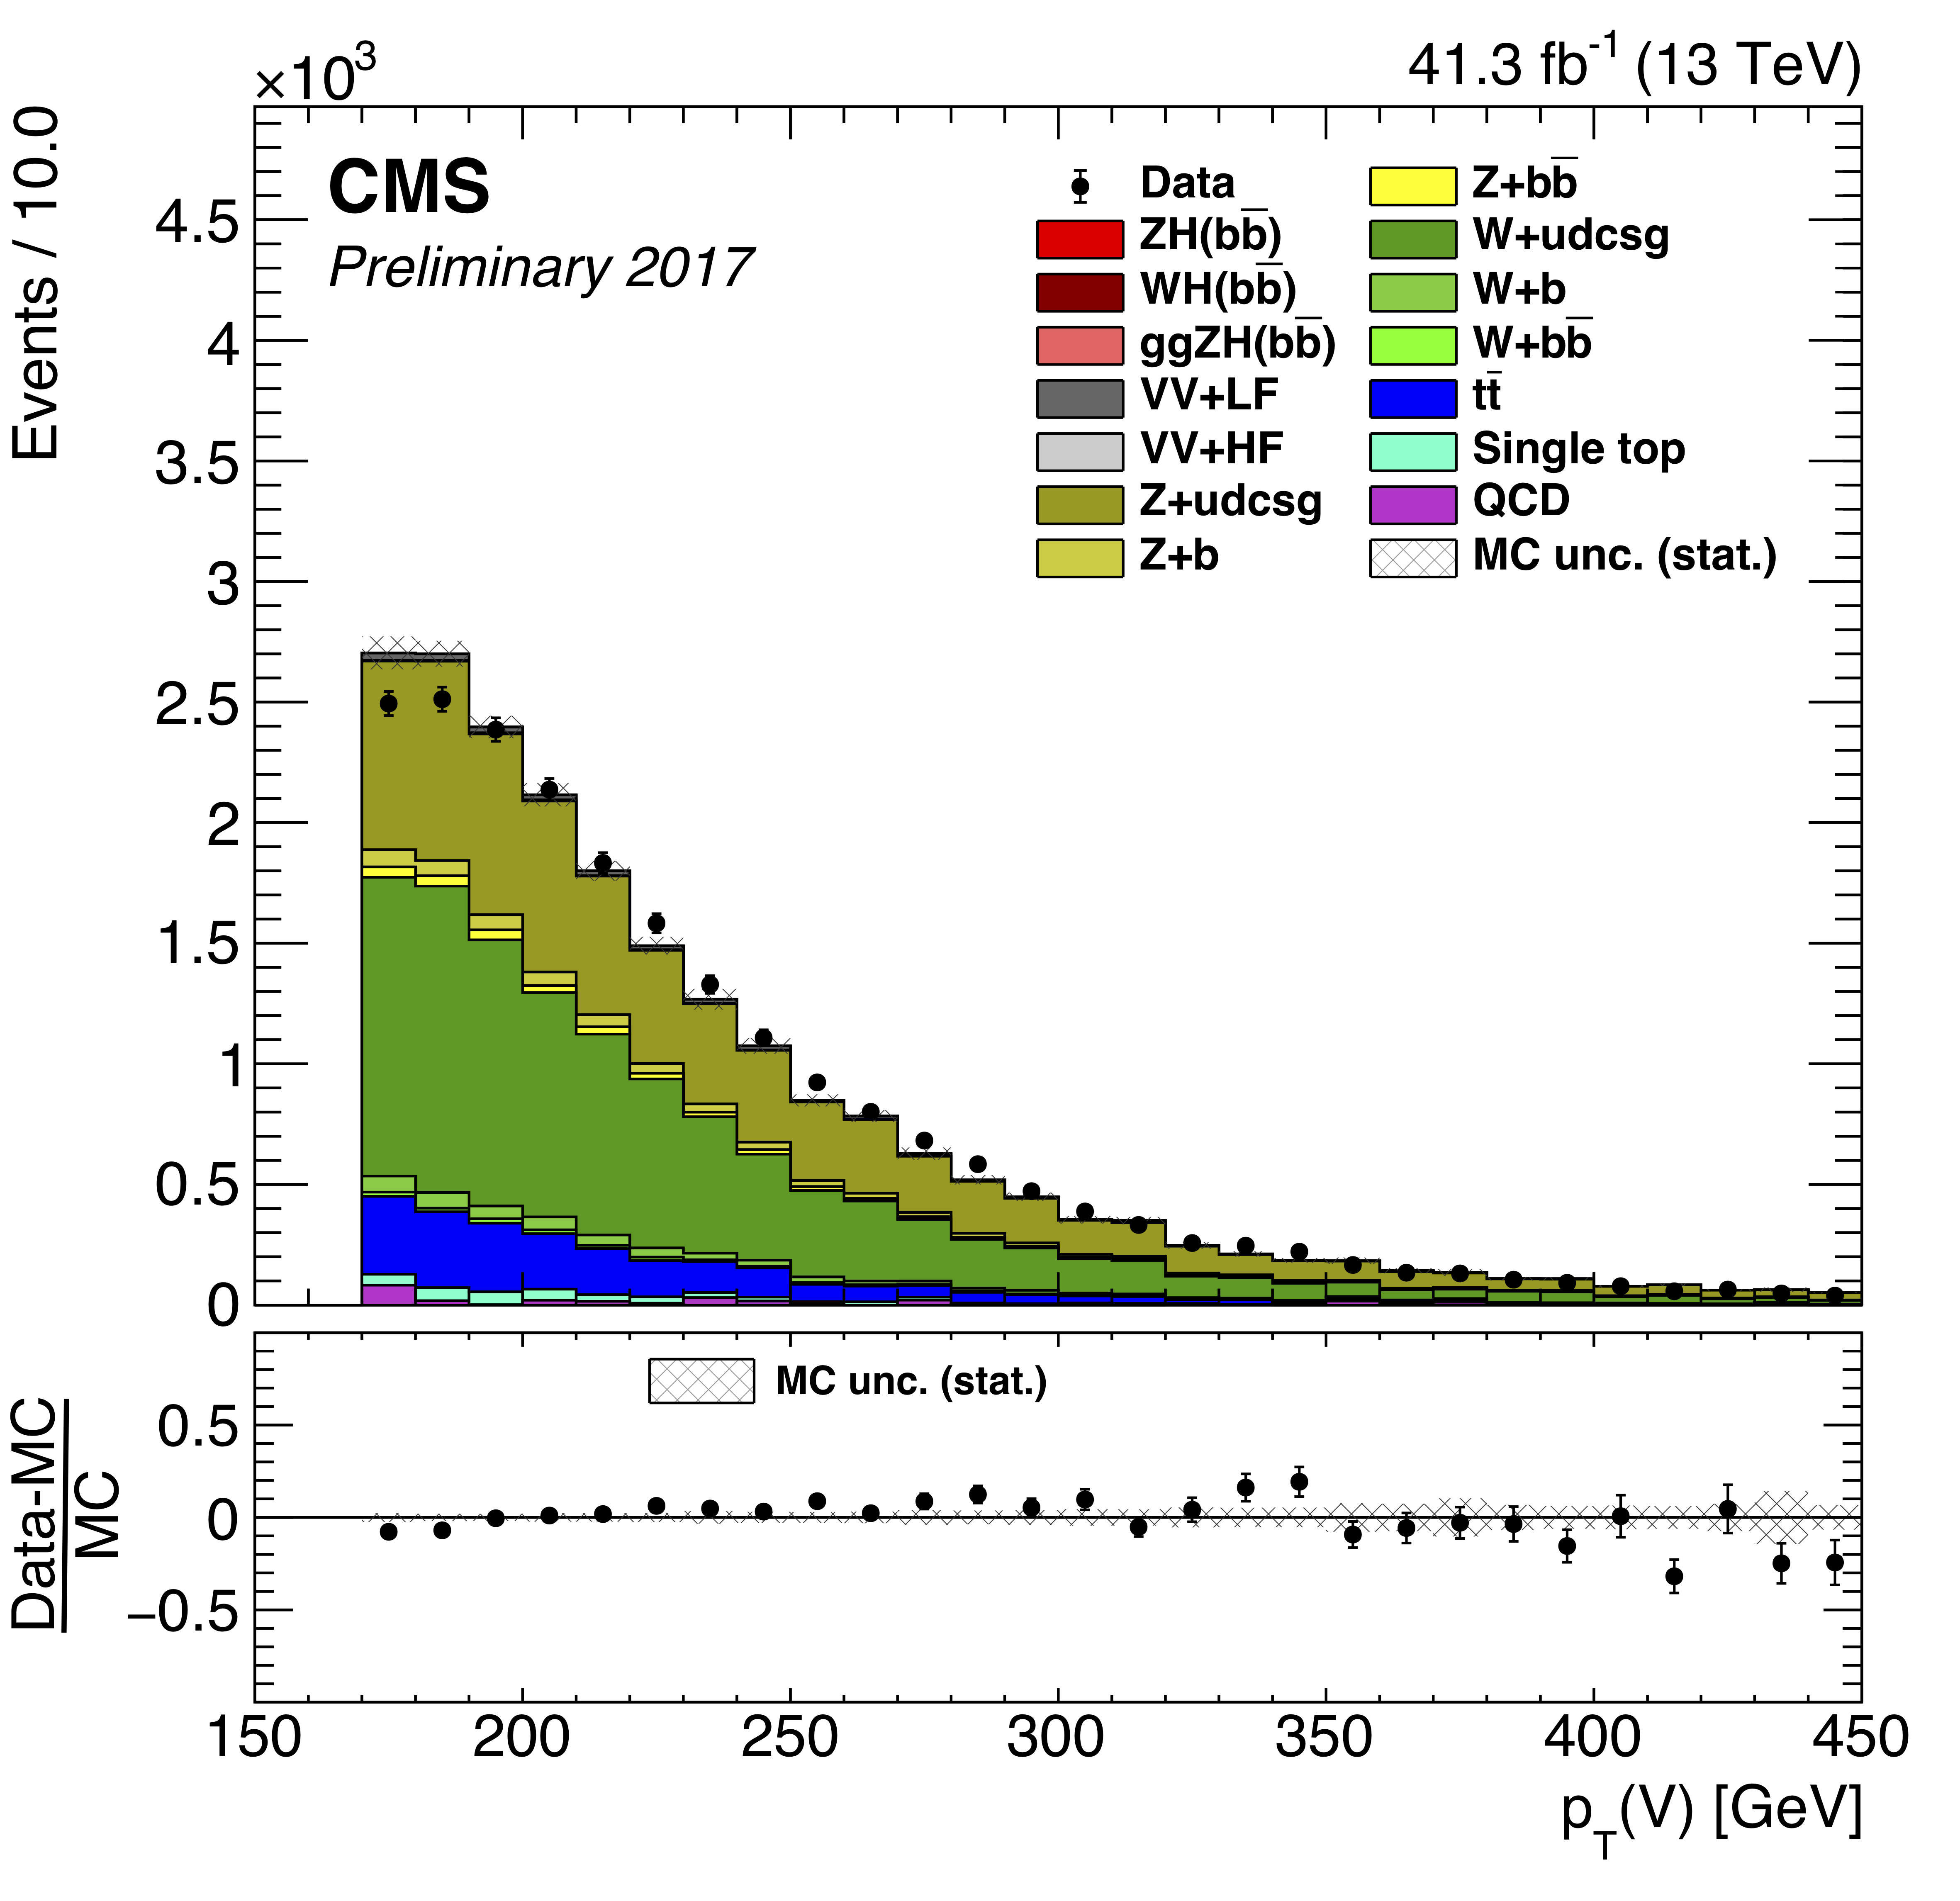
\includegraphics[width=0.39\linewidth]{images/CR_Znn_ZLF/V_pt}}
    \subfigure [] {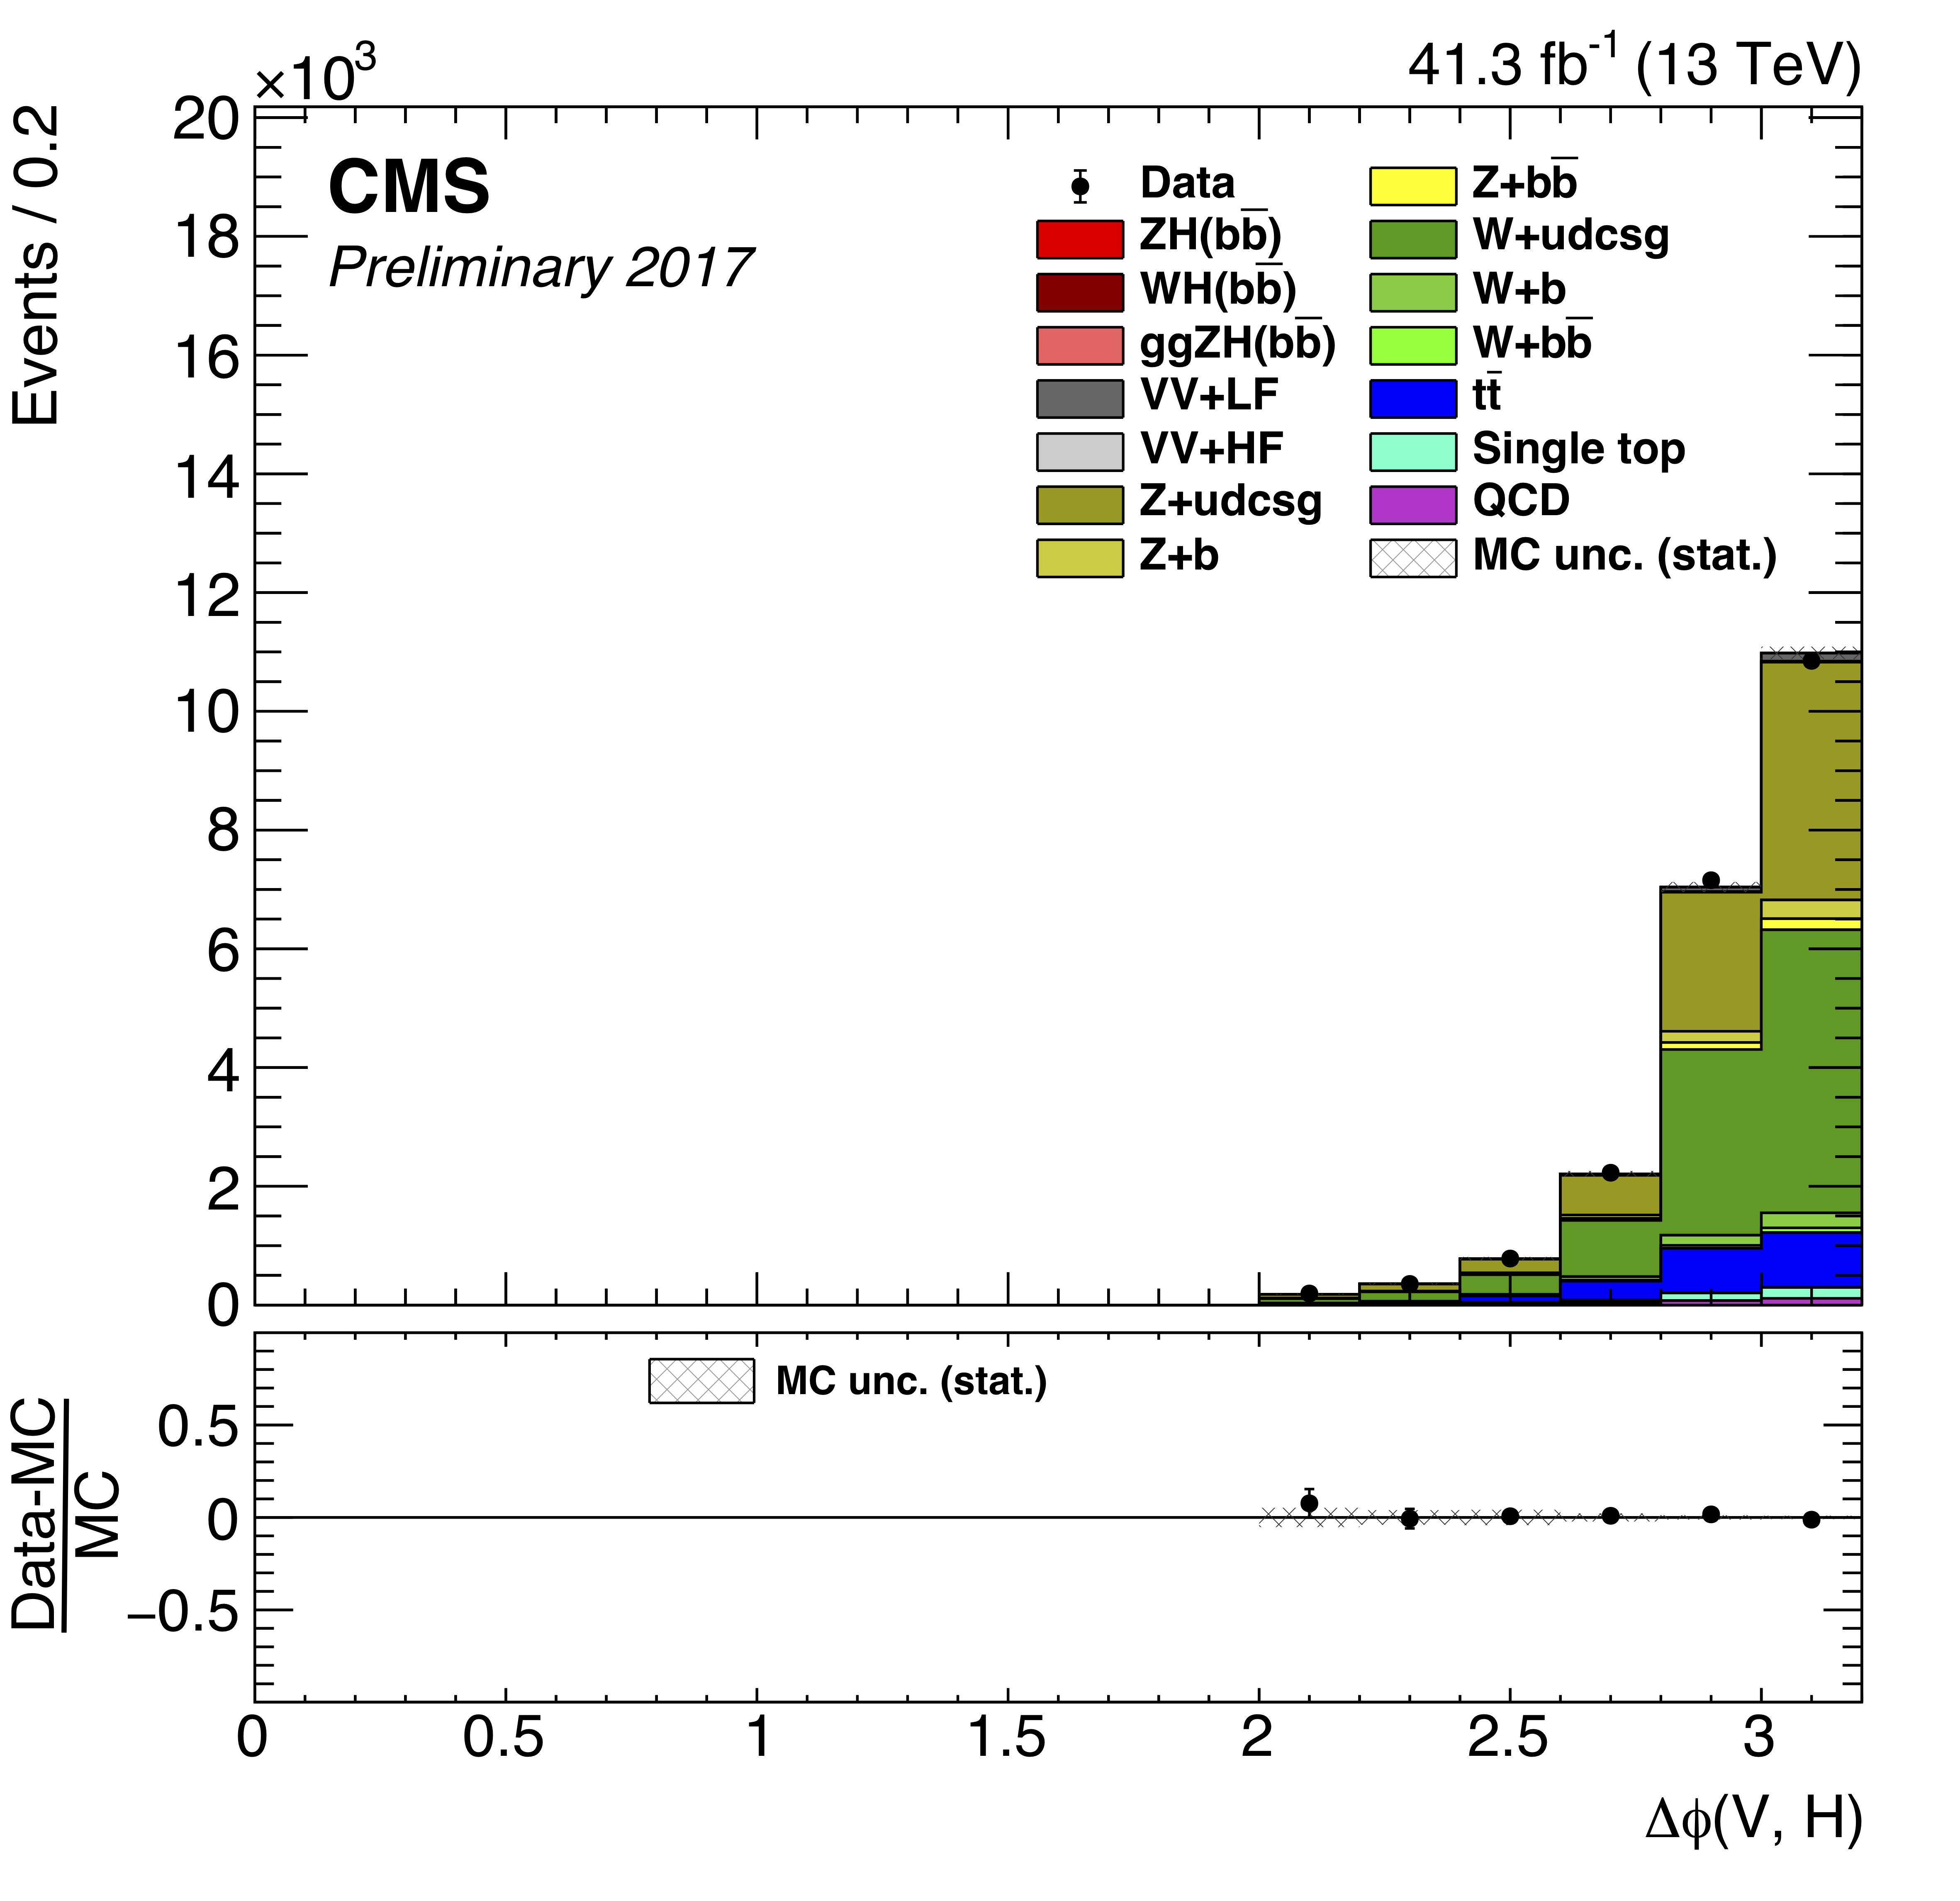
\includegraphics[width=0.39\linewidth]{images/CR_Znn_ZLF/HVdPhi}}
  }
  \mbox{
    \subfigure [] {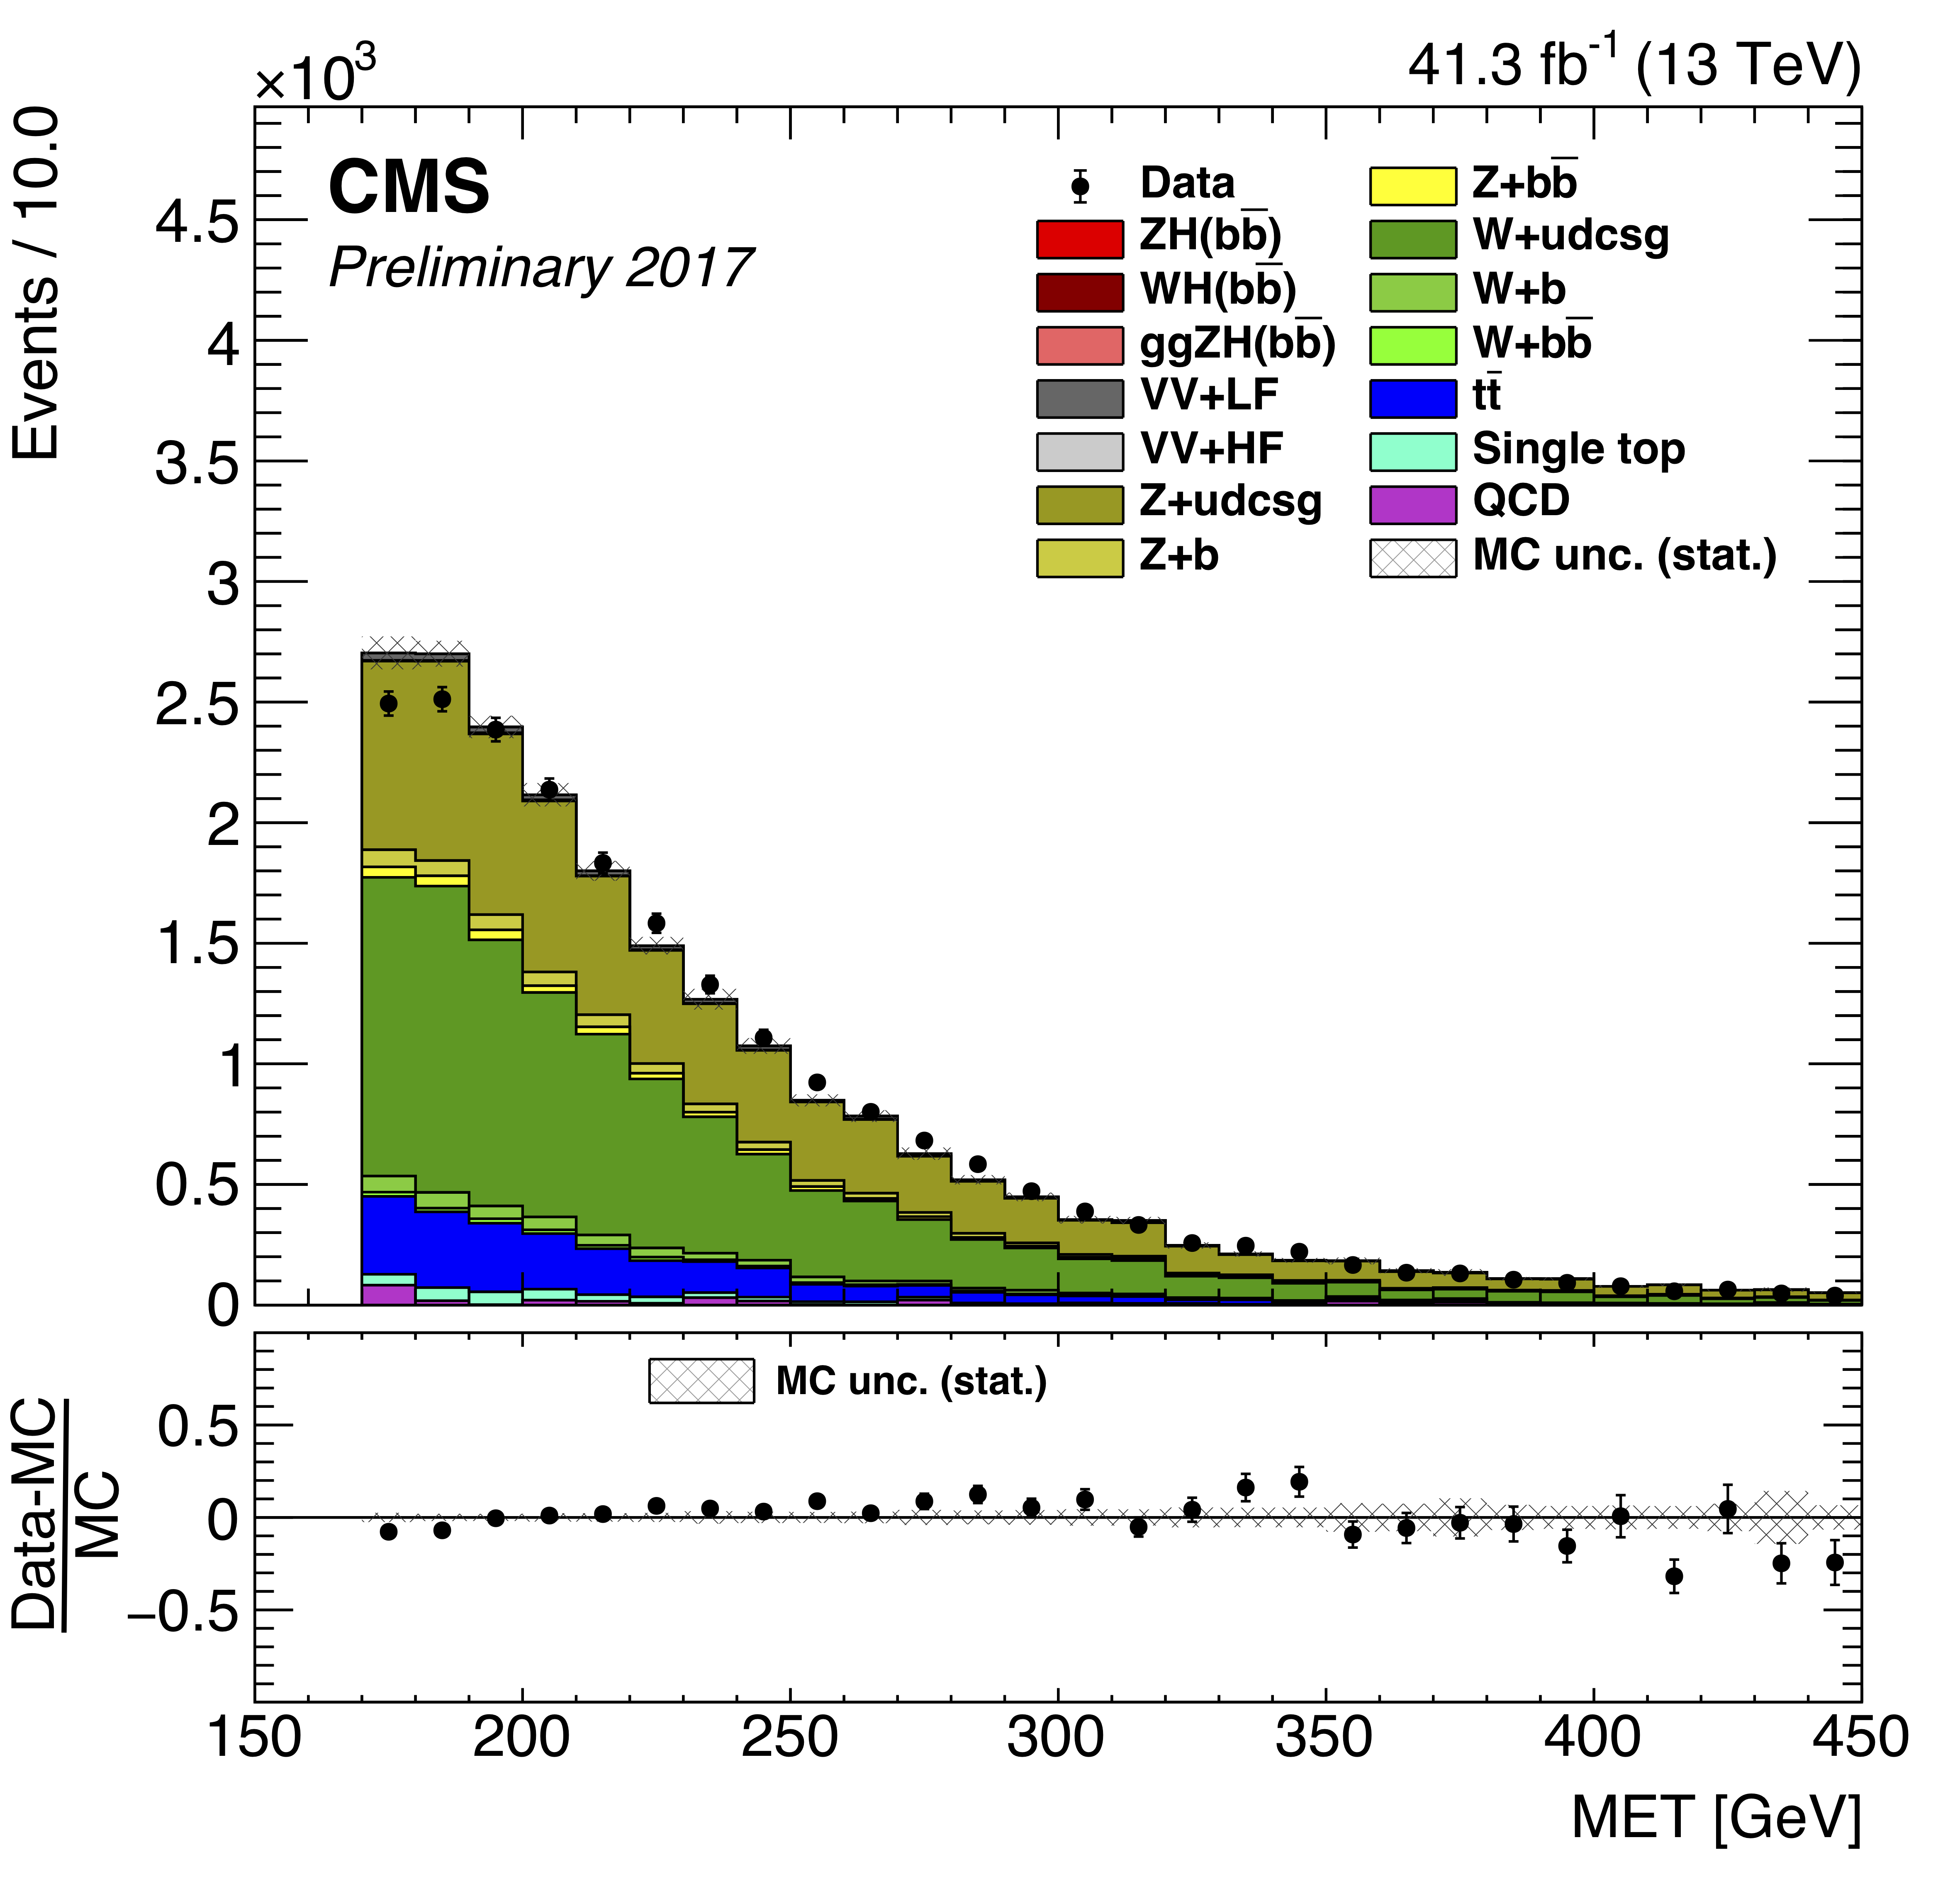
\includegraphics[width=0.39\linewidth]{images/CR_Znn_ZLF/MET_Pt}}
    \subfigure [] {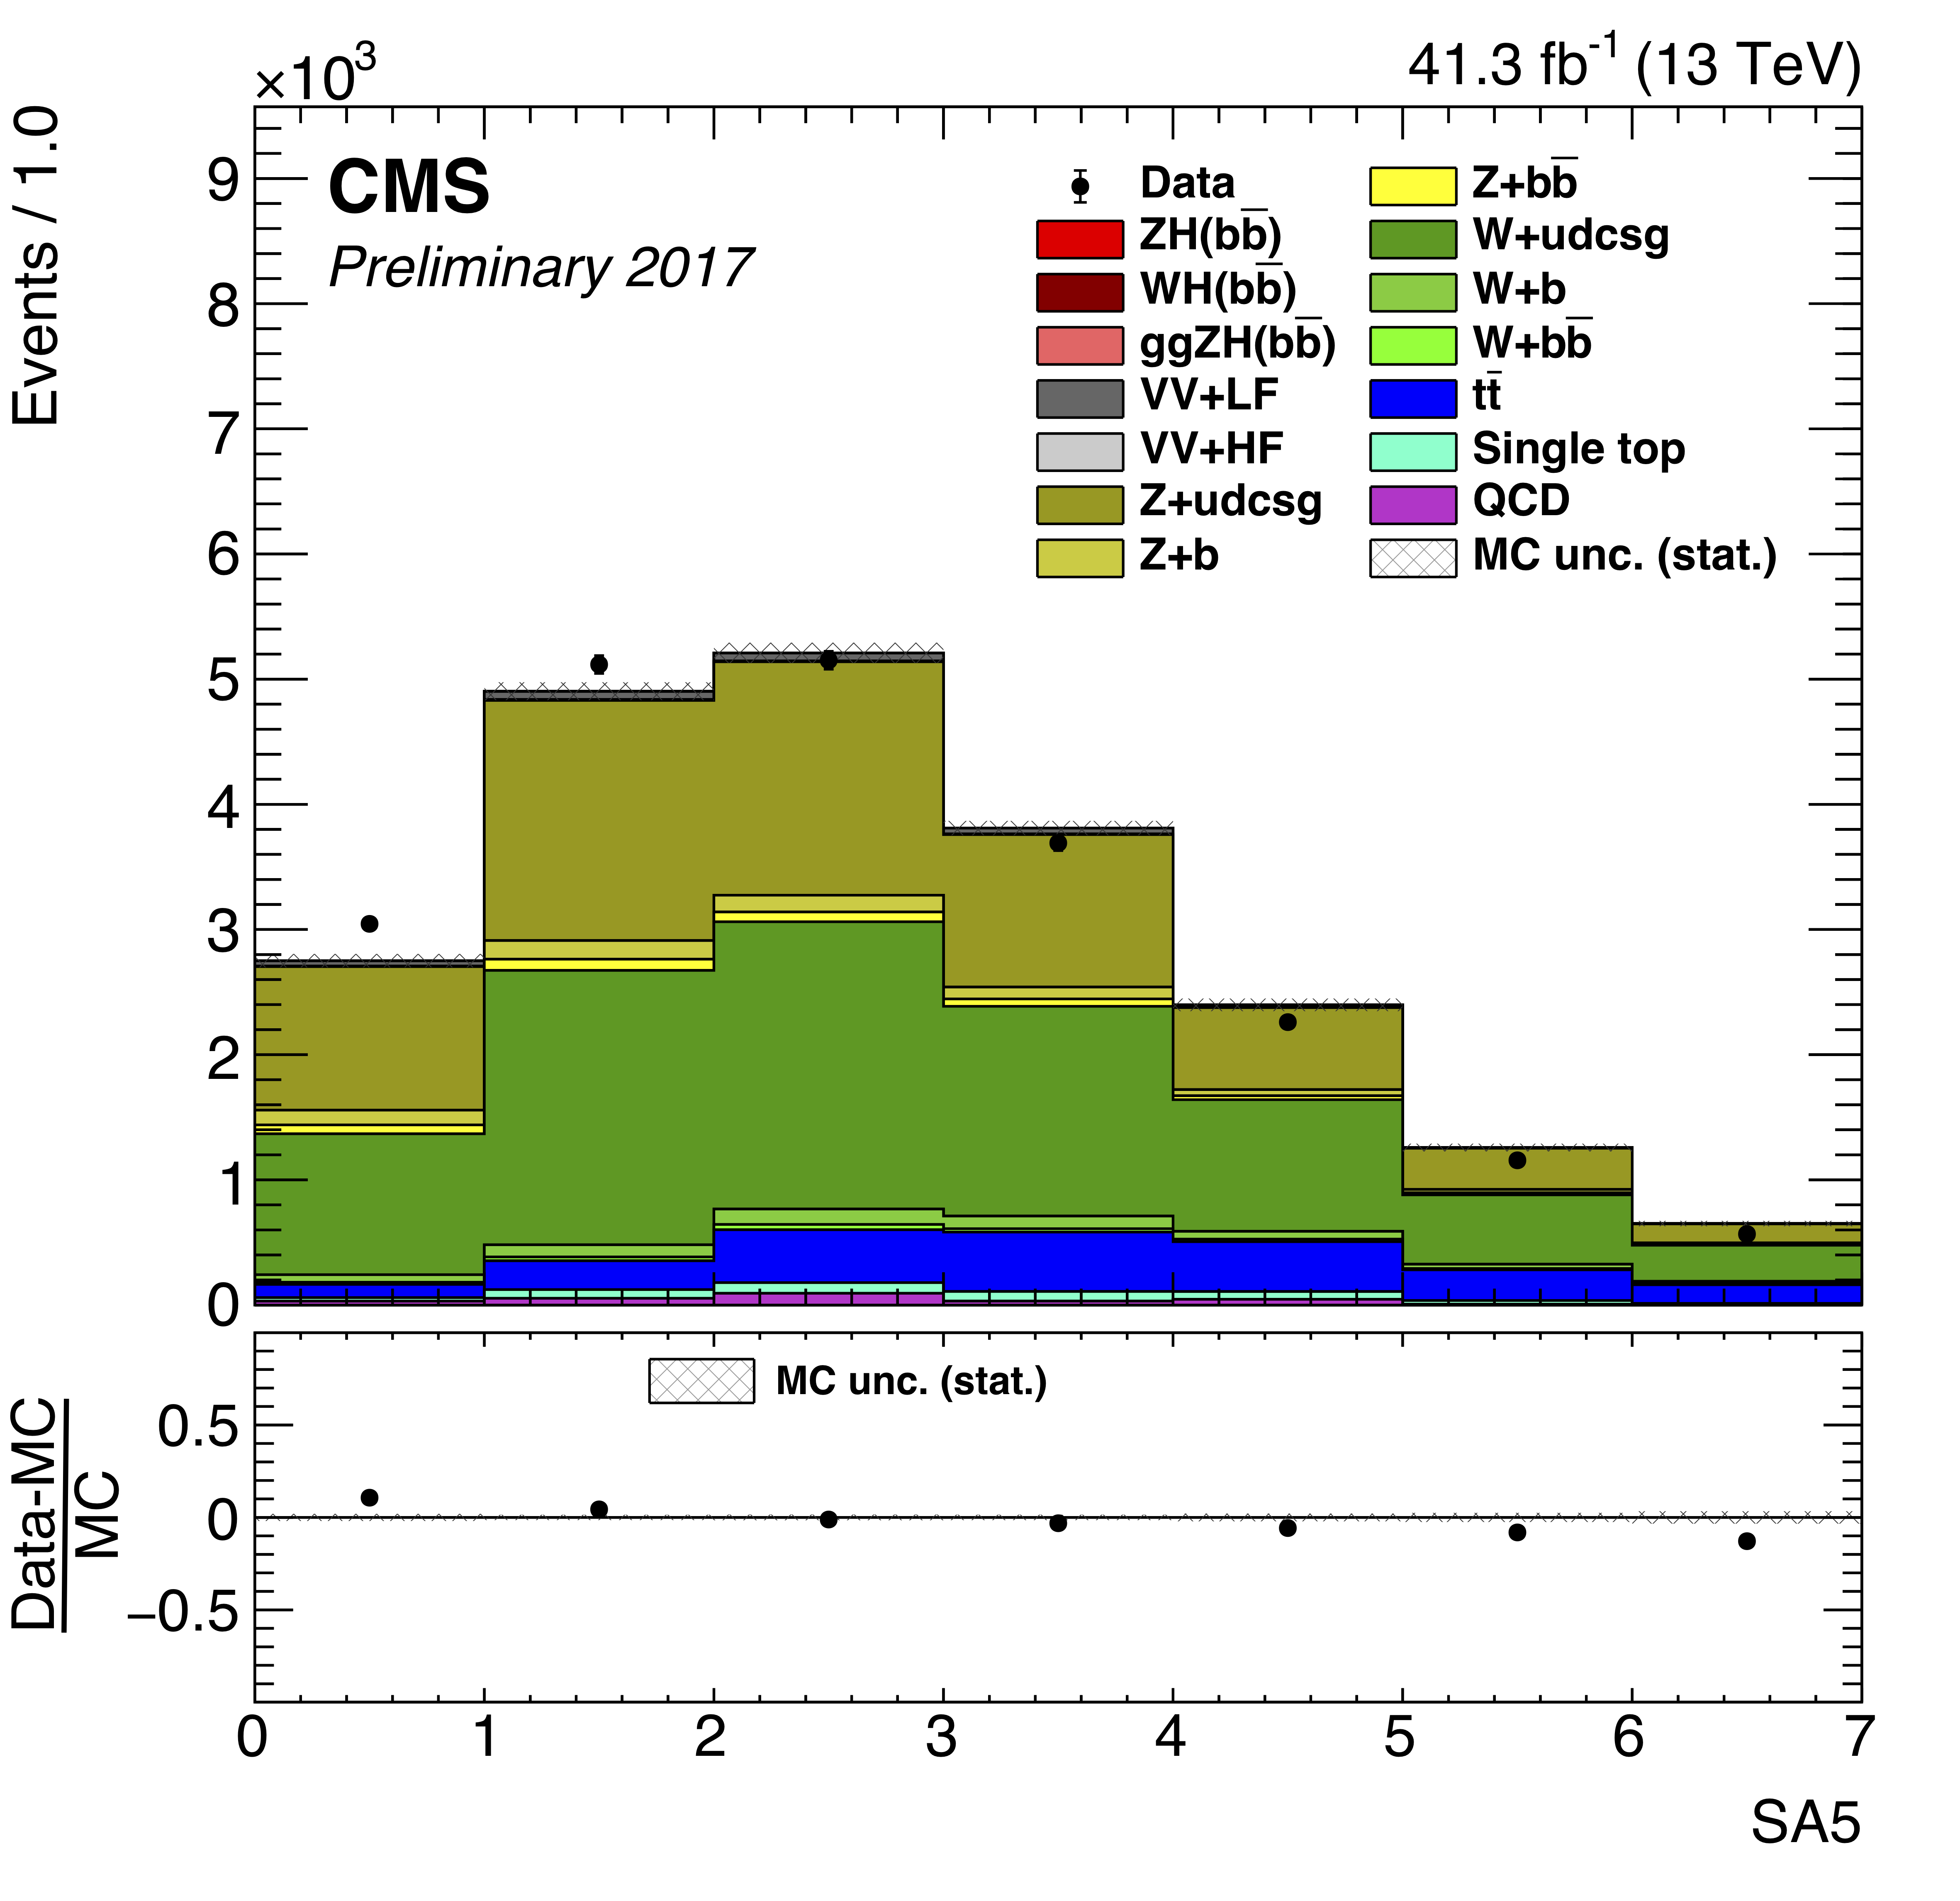
\includegraphics[width=0.39\linewidth]{images/CR_Znn_ZLF/SA5}}
  }
  \caption[Additional \bosZ+light Control Region Distributions for the \ZnnH\ Channel]{The distributions of variables in the \bosZ+light control region of the \ZnnH\ channel: A) $\left| \Delta \eta (j_{1}, j_{2}) \right|$, B) $\left| \Delta \phi (j_{1}, j_{2}) \right|$, C) $\pT(\bosV)$, D) $\left| \Delta \phi (\bosV, \bosH) \right|$, E) \pTmiss, F) SA5.}
  \label{fig:CR_Znn_ZLF_2}
\end{figure}

\clearpage

% Z+heavy

\begin{figure}[htbp]
  \centering
  \mbox{
    \subfigure [] {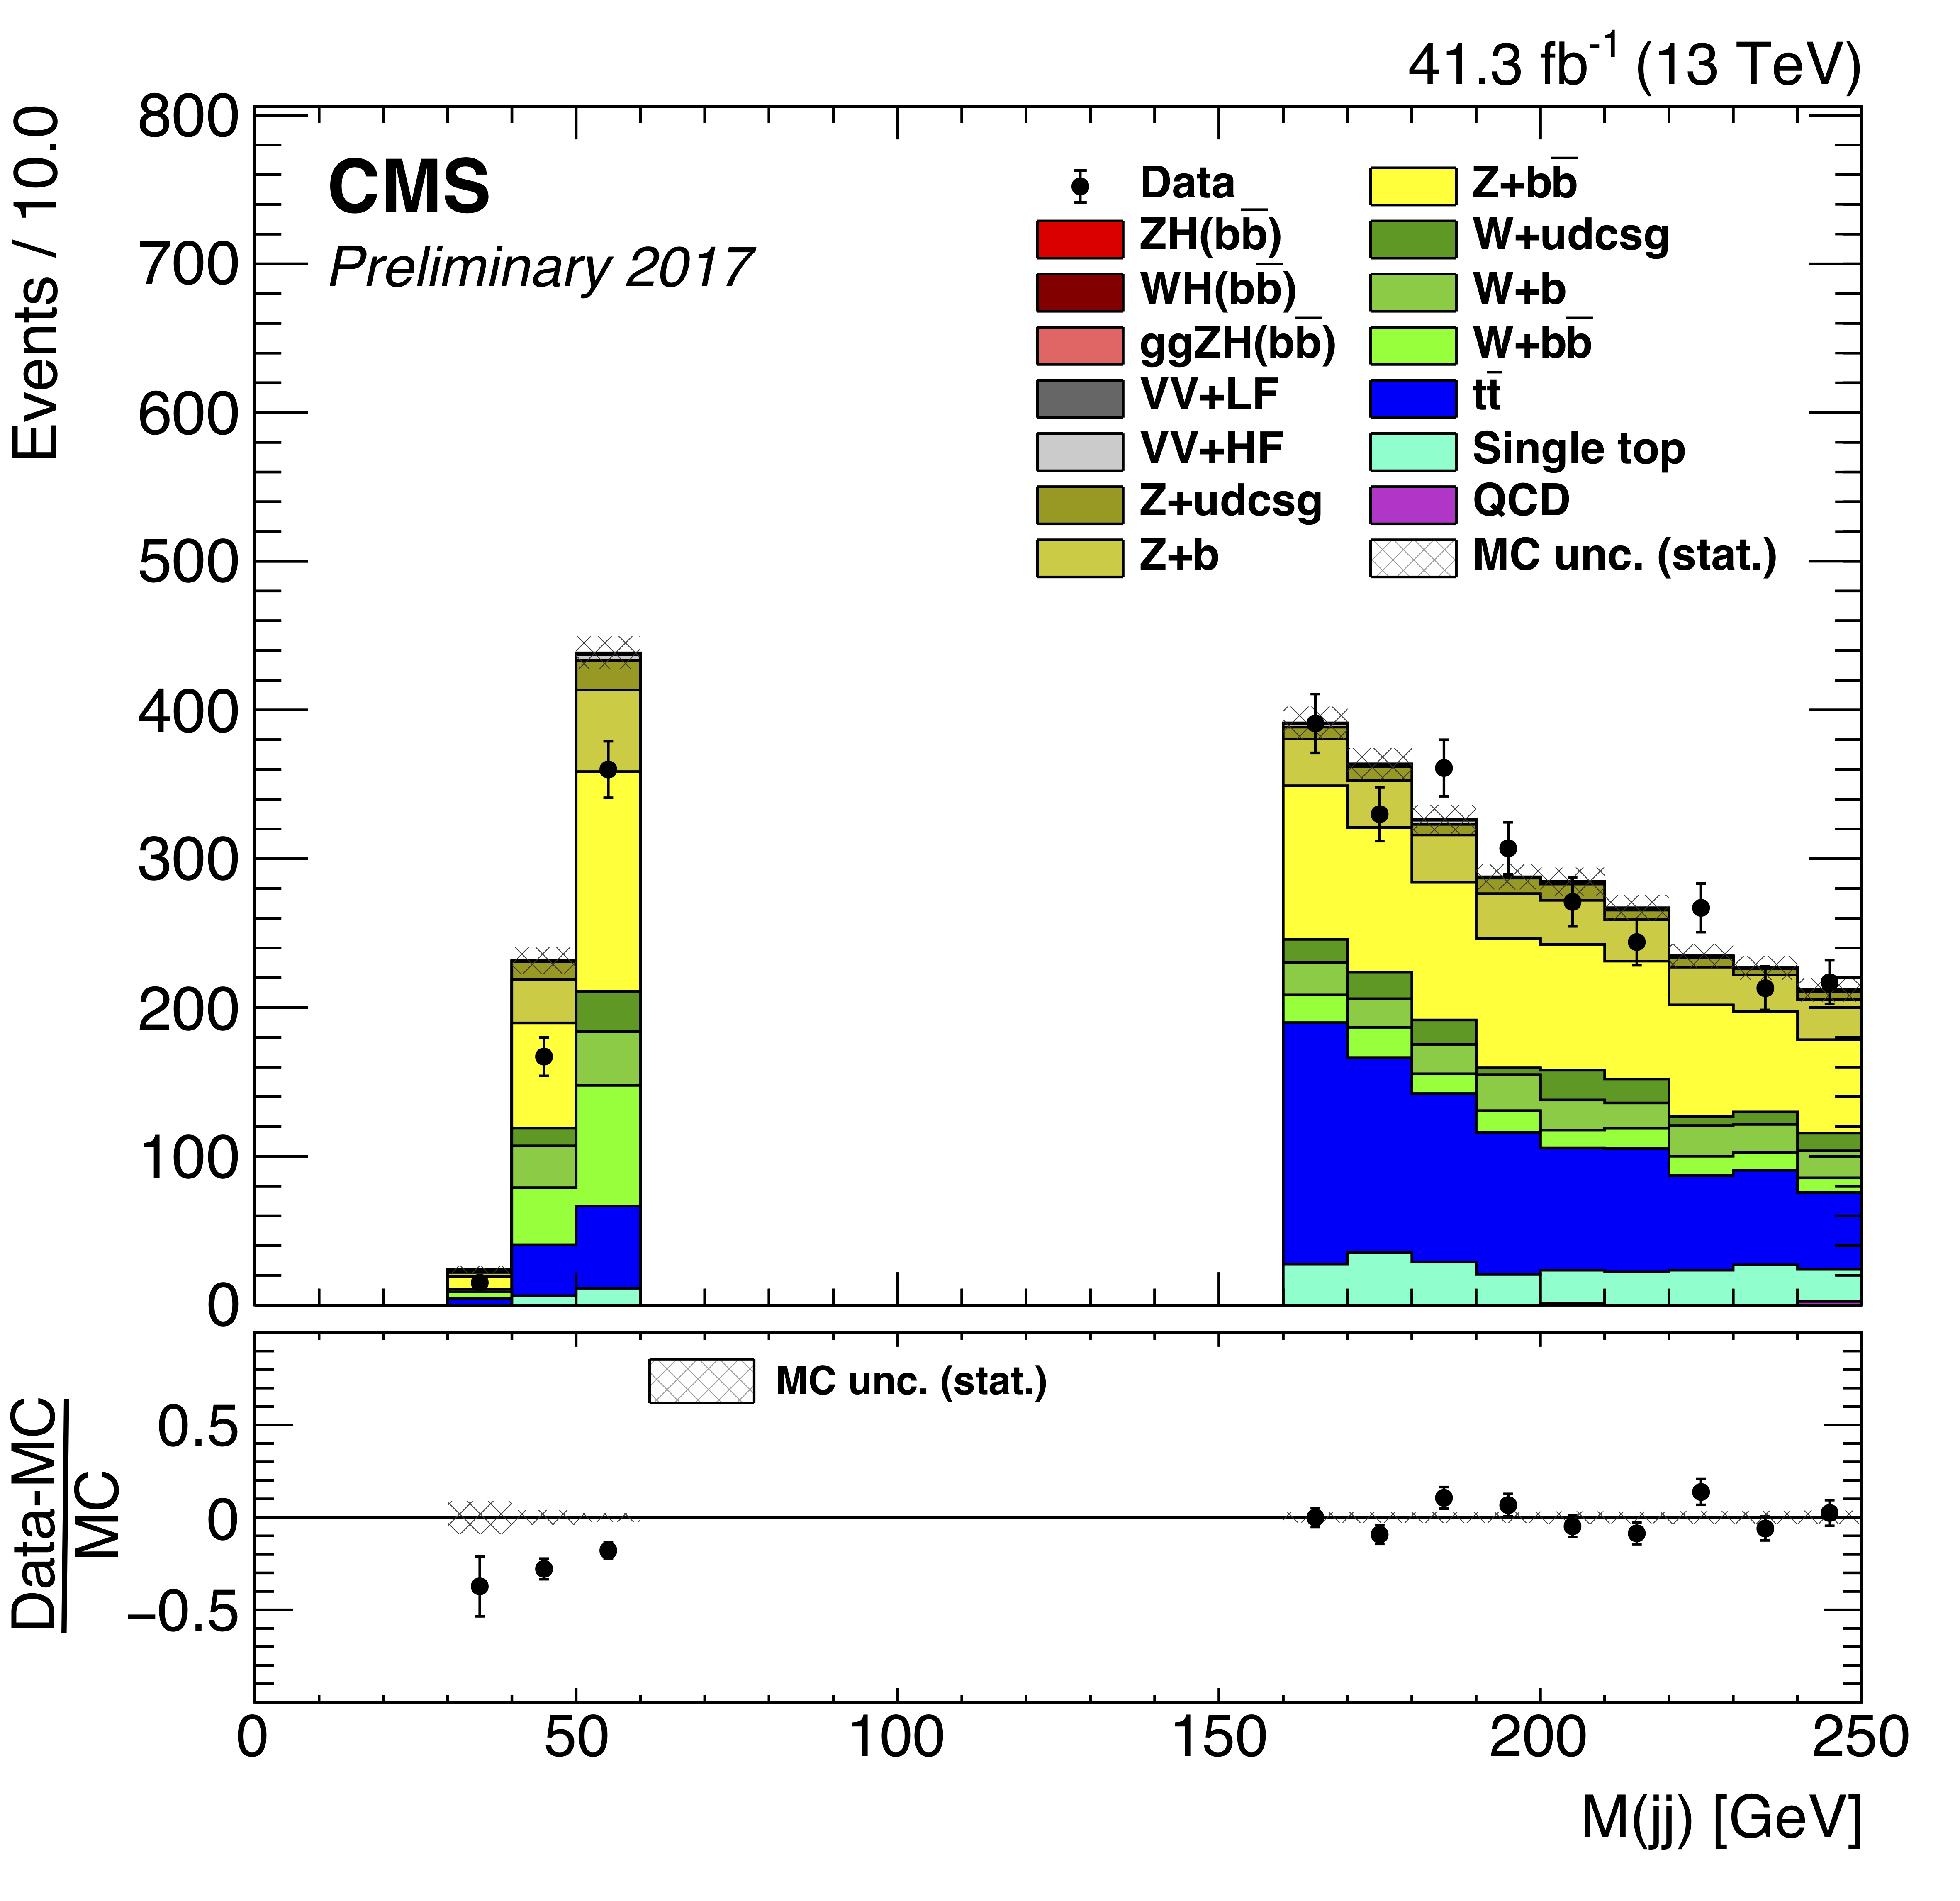
\includegraphics[width=0.39\linewidth]{images/CR_Znn_ZHF/H_mass}}
    \subfigure [] {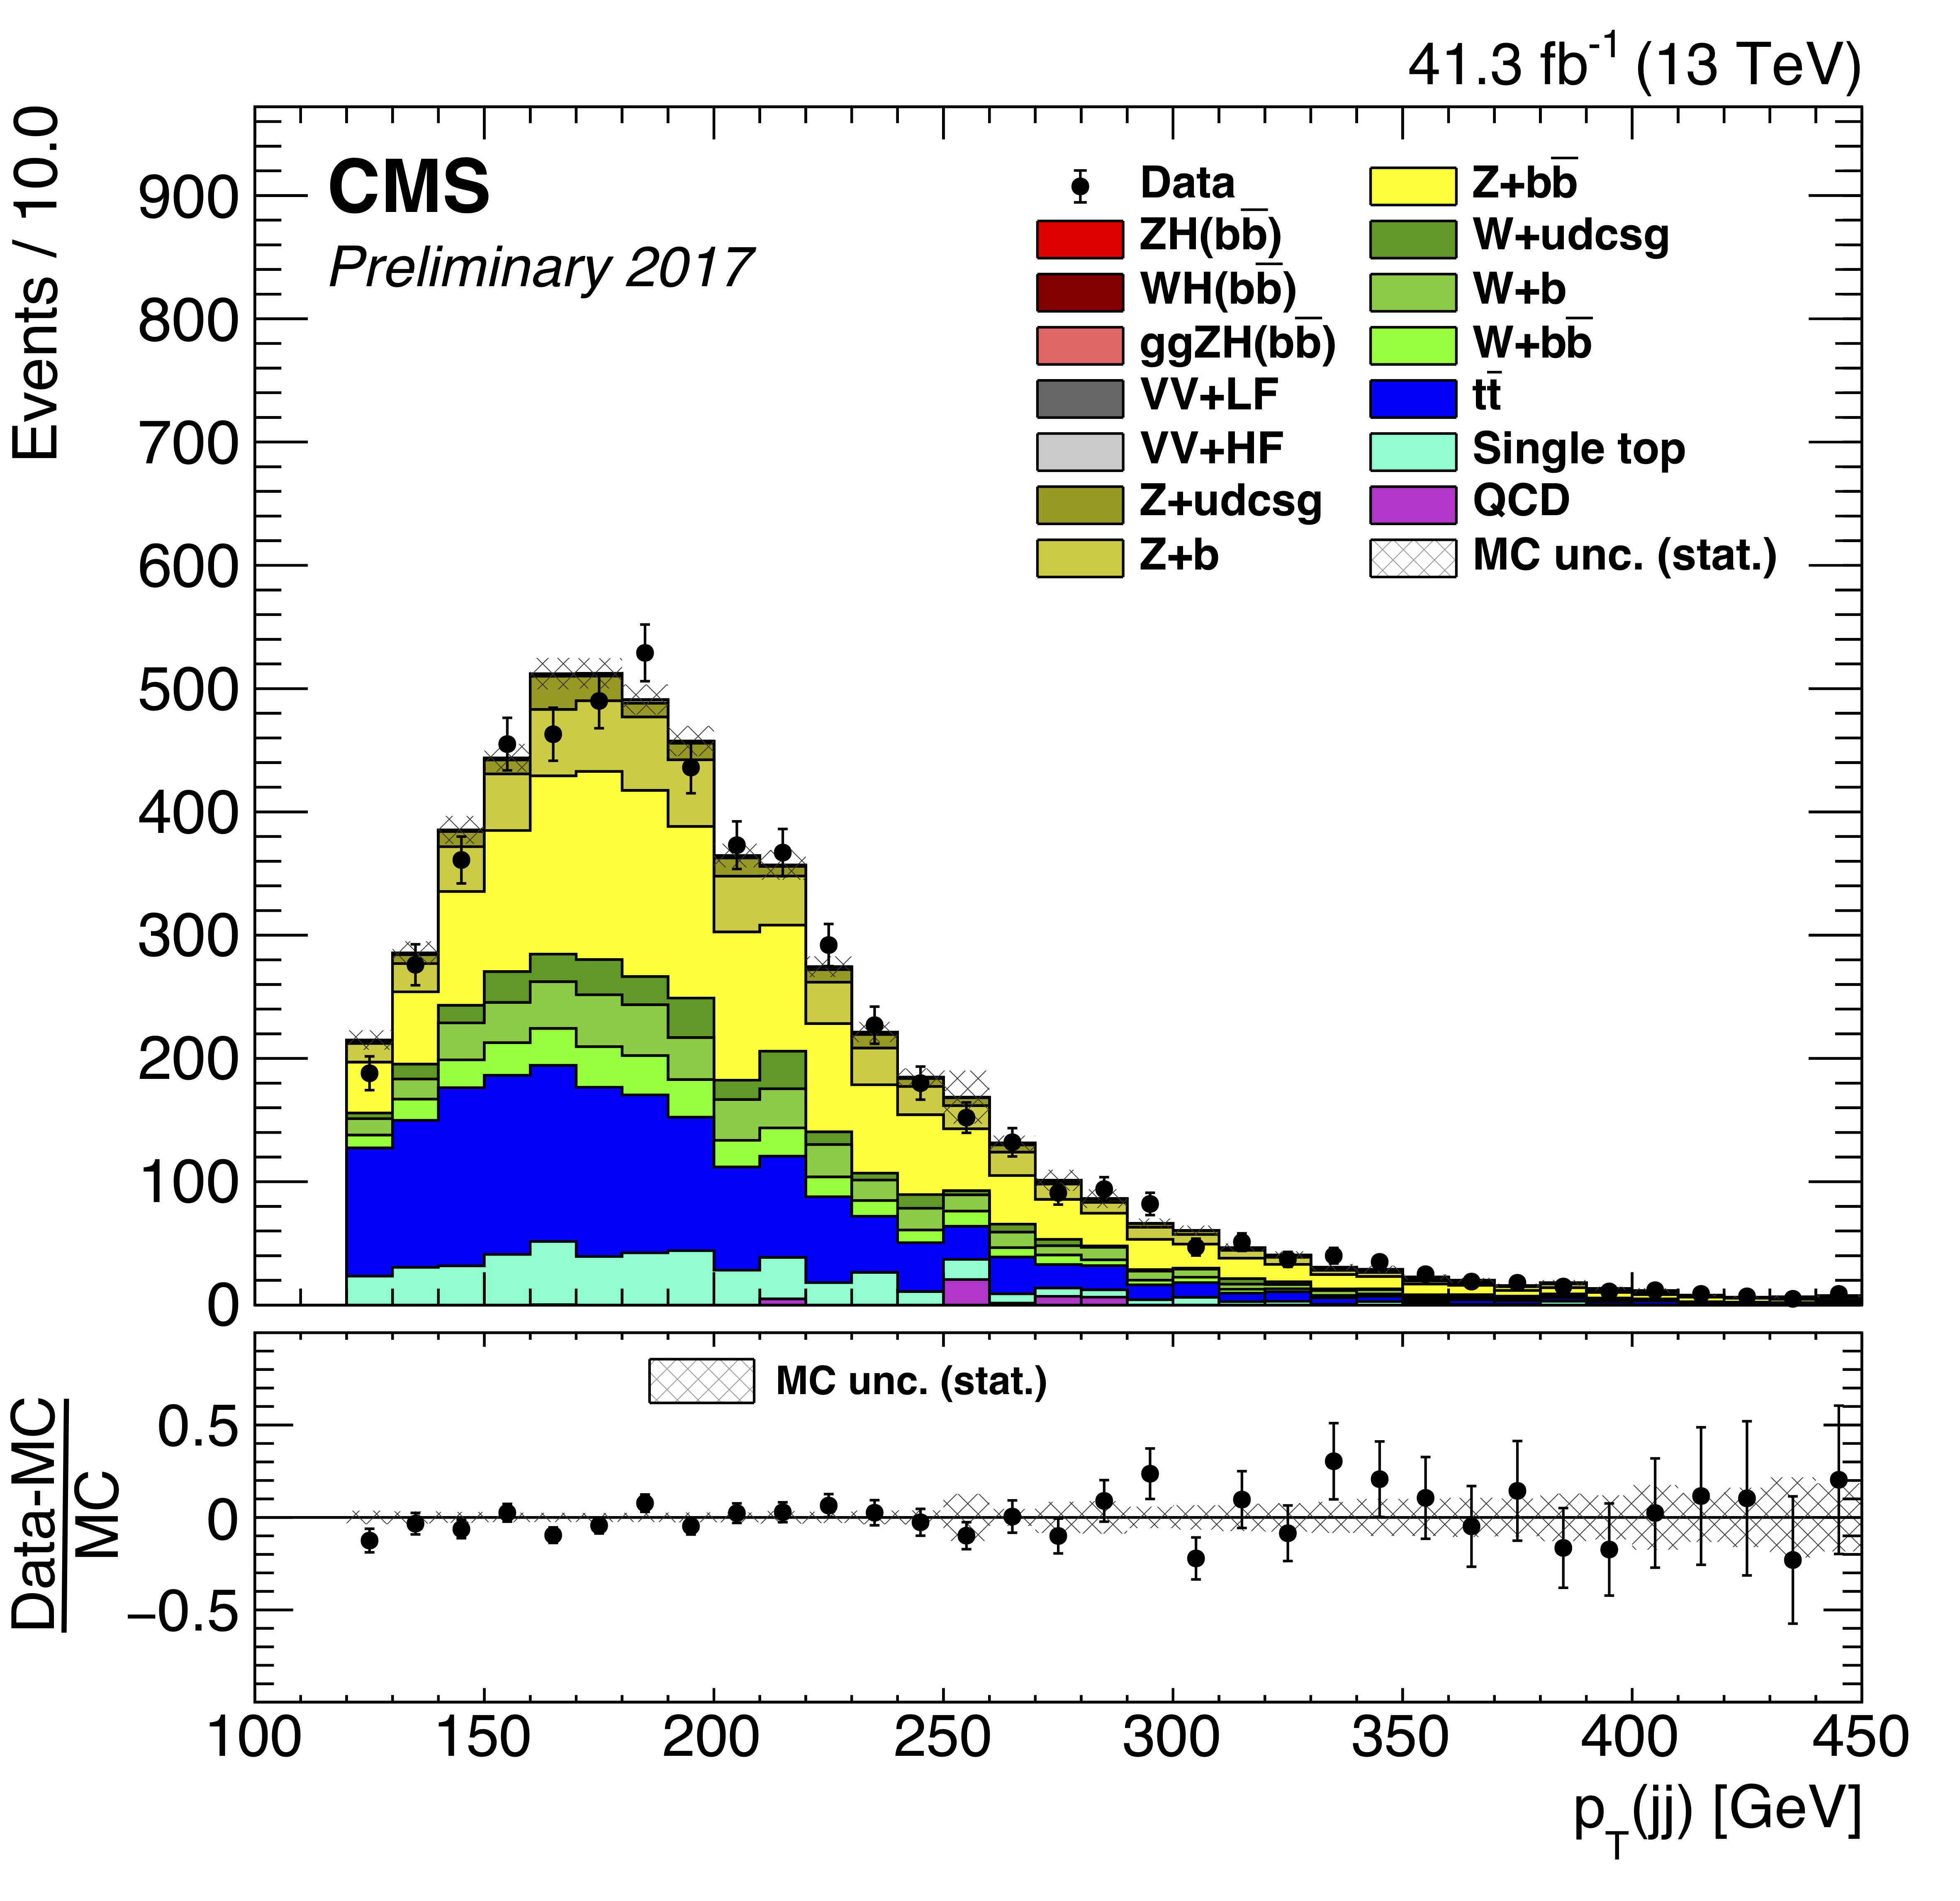
\includegraphics[width=0.39\linewidth]{images/CR_Znn_ZHF/H_pt}}
  }
  \mbox{
    \subfigure [] {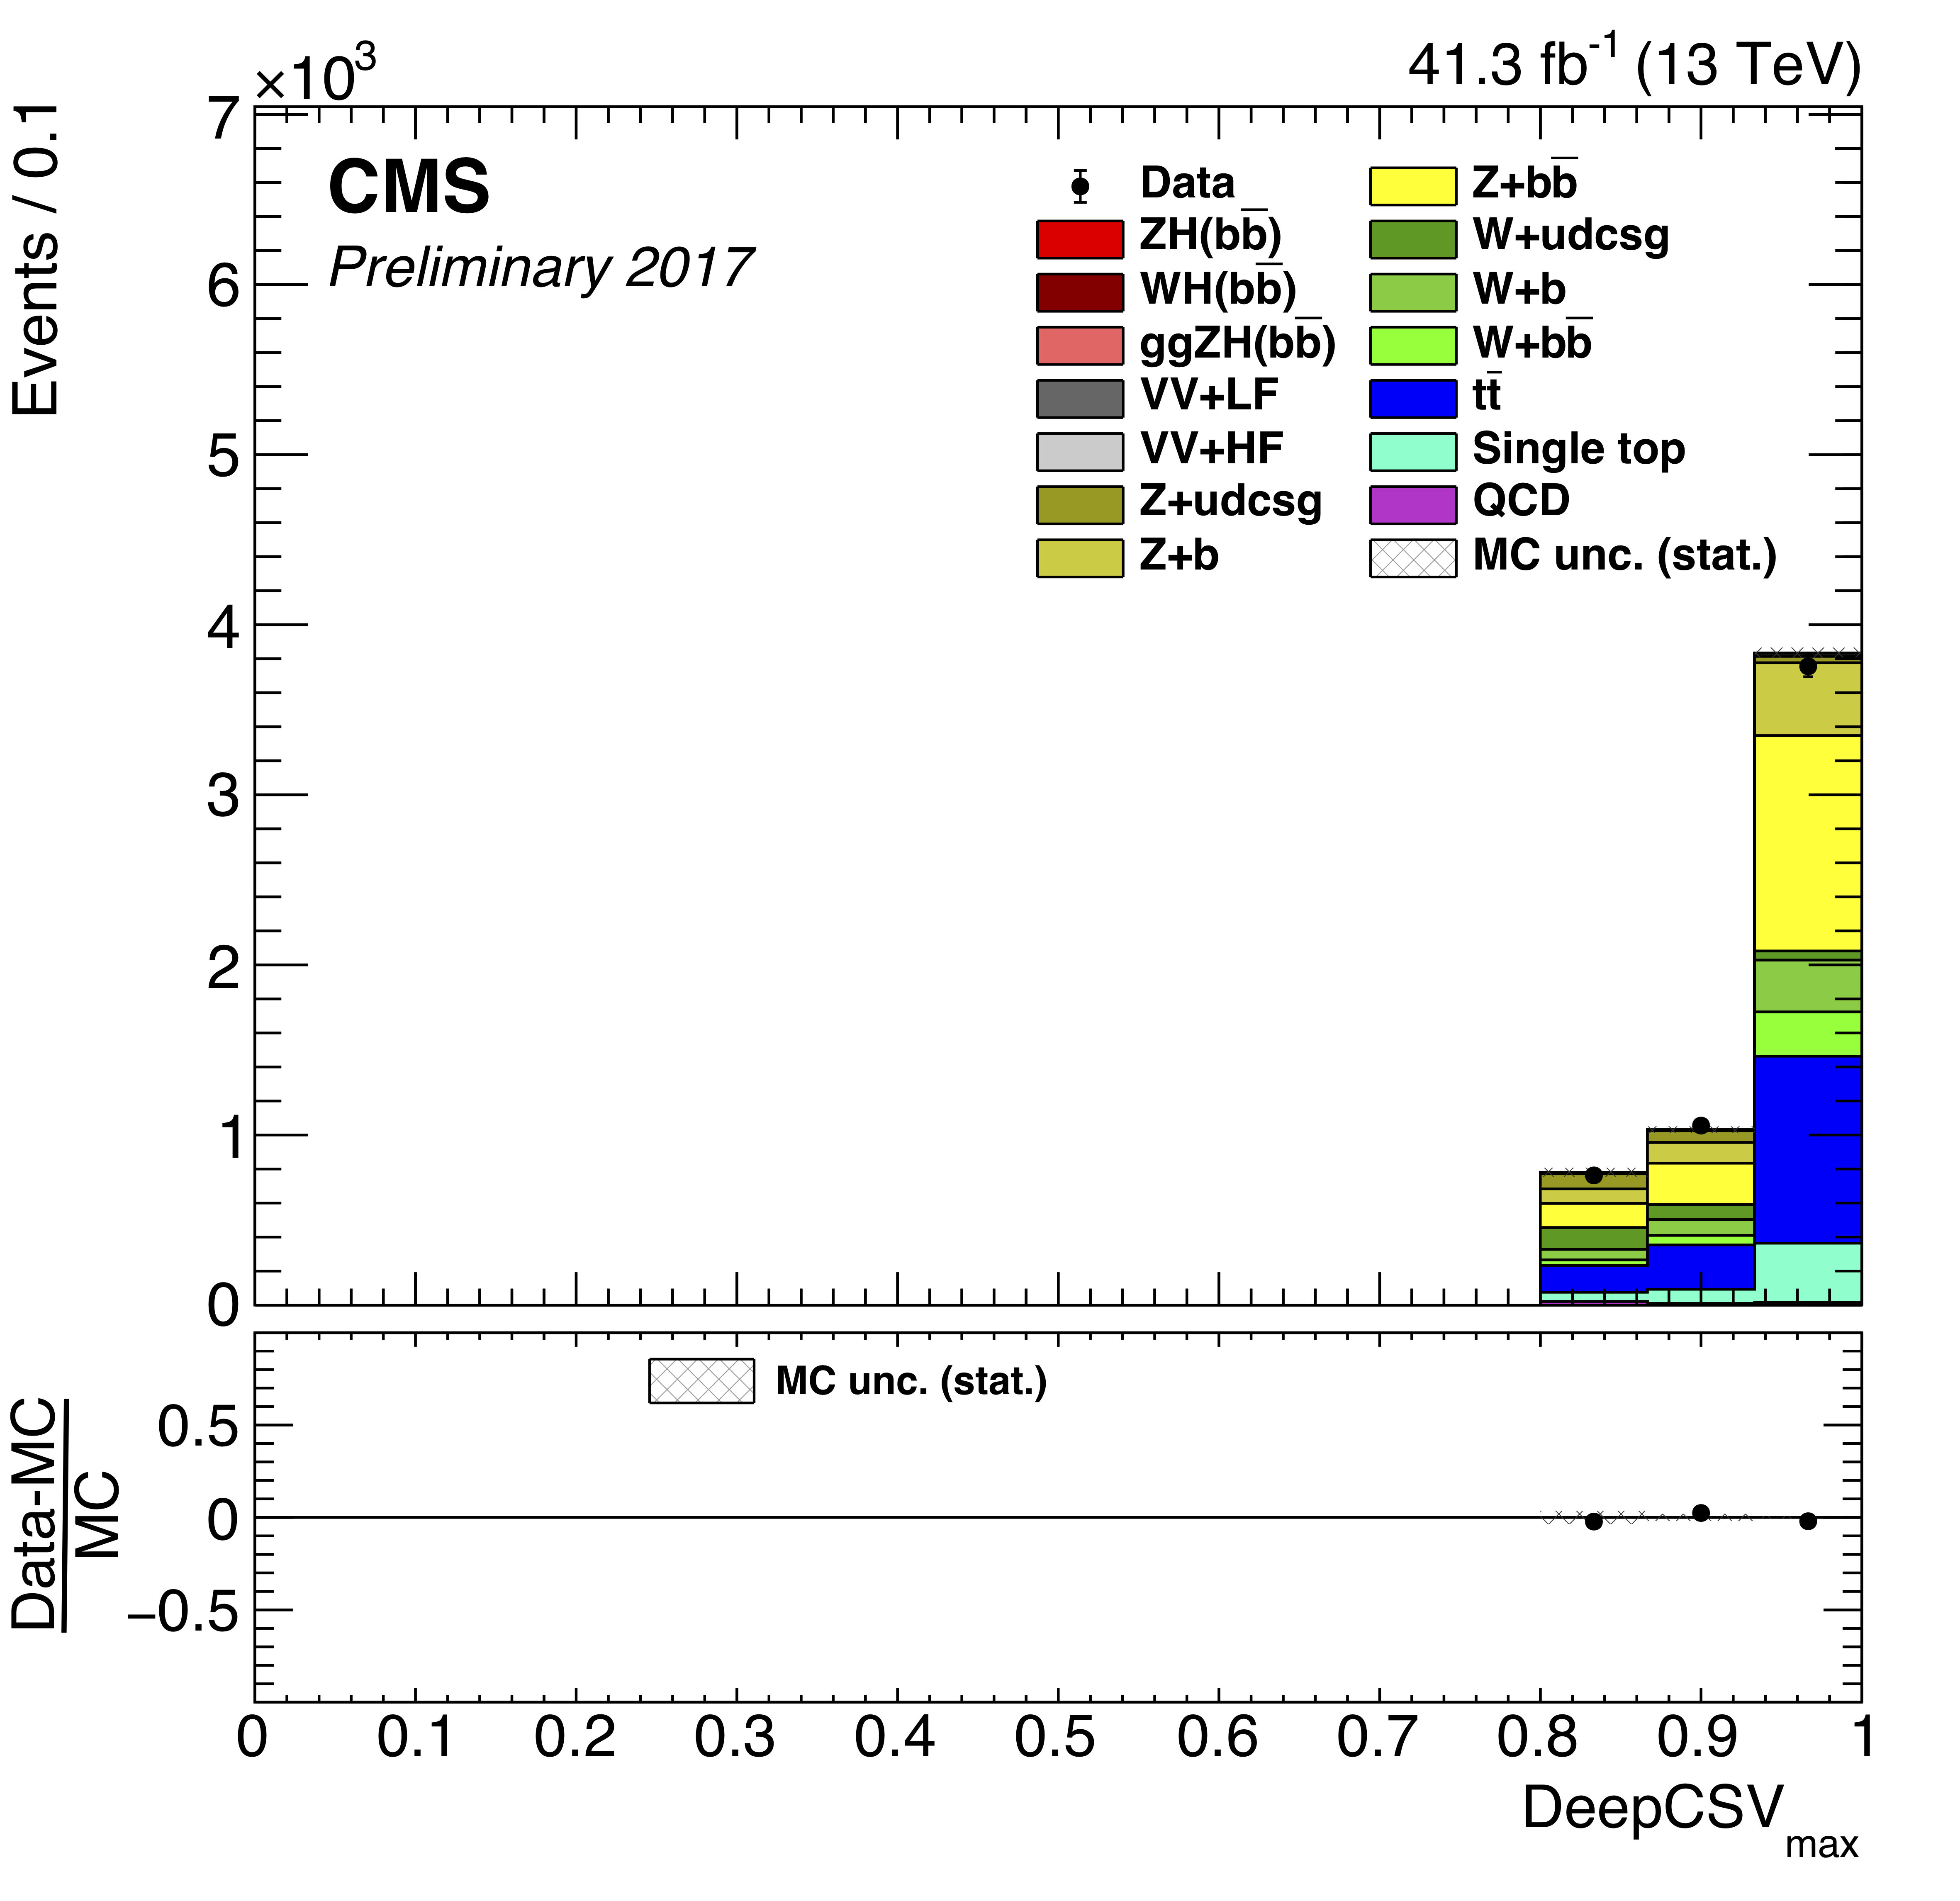
\includegraphics[width=0.39\linewidth]{images/CR_Znn_ZHF/hJets_DeepCSV_0}}
    \subfigure [] {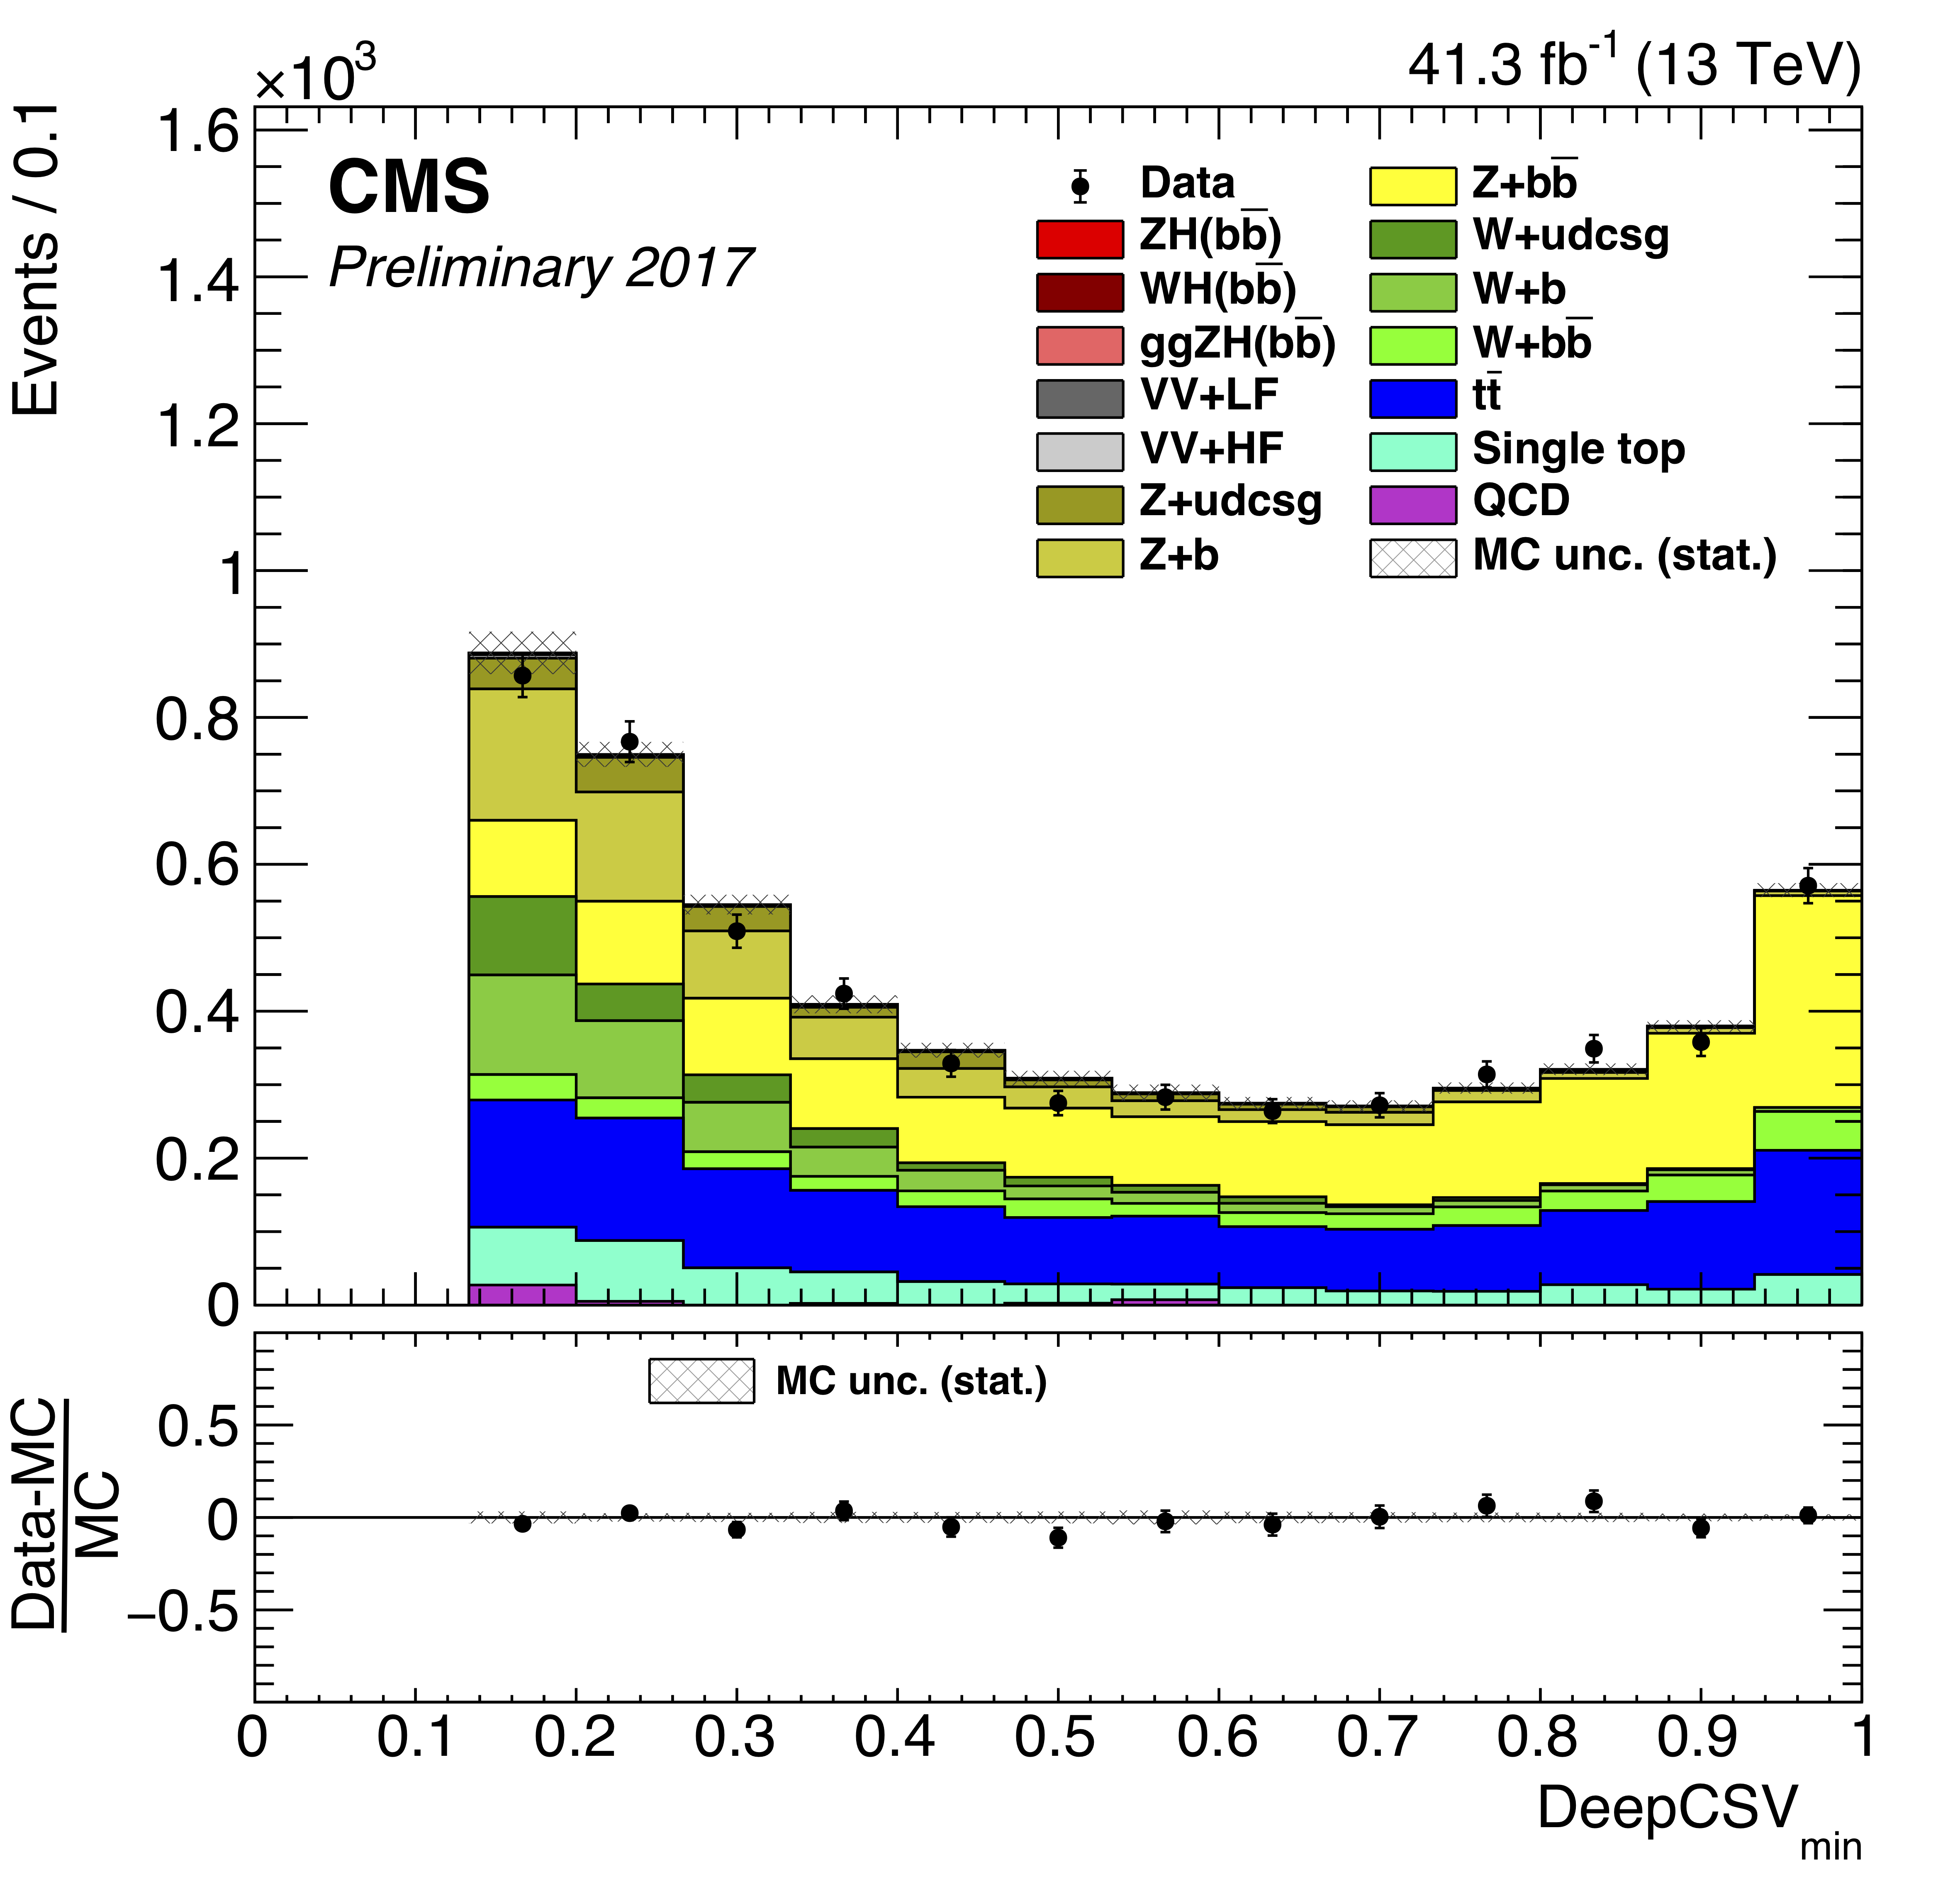
\includegraphics[width=0.39\linewidth]{images/CR_Znn_ZHF/hJets_DeepCSV_1}}
  }
  \mbox{
    \subfigure [] {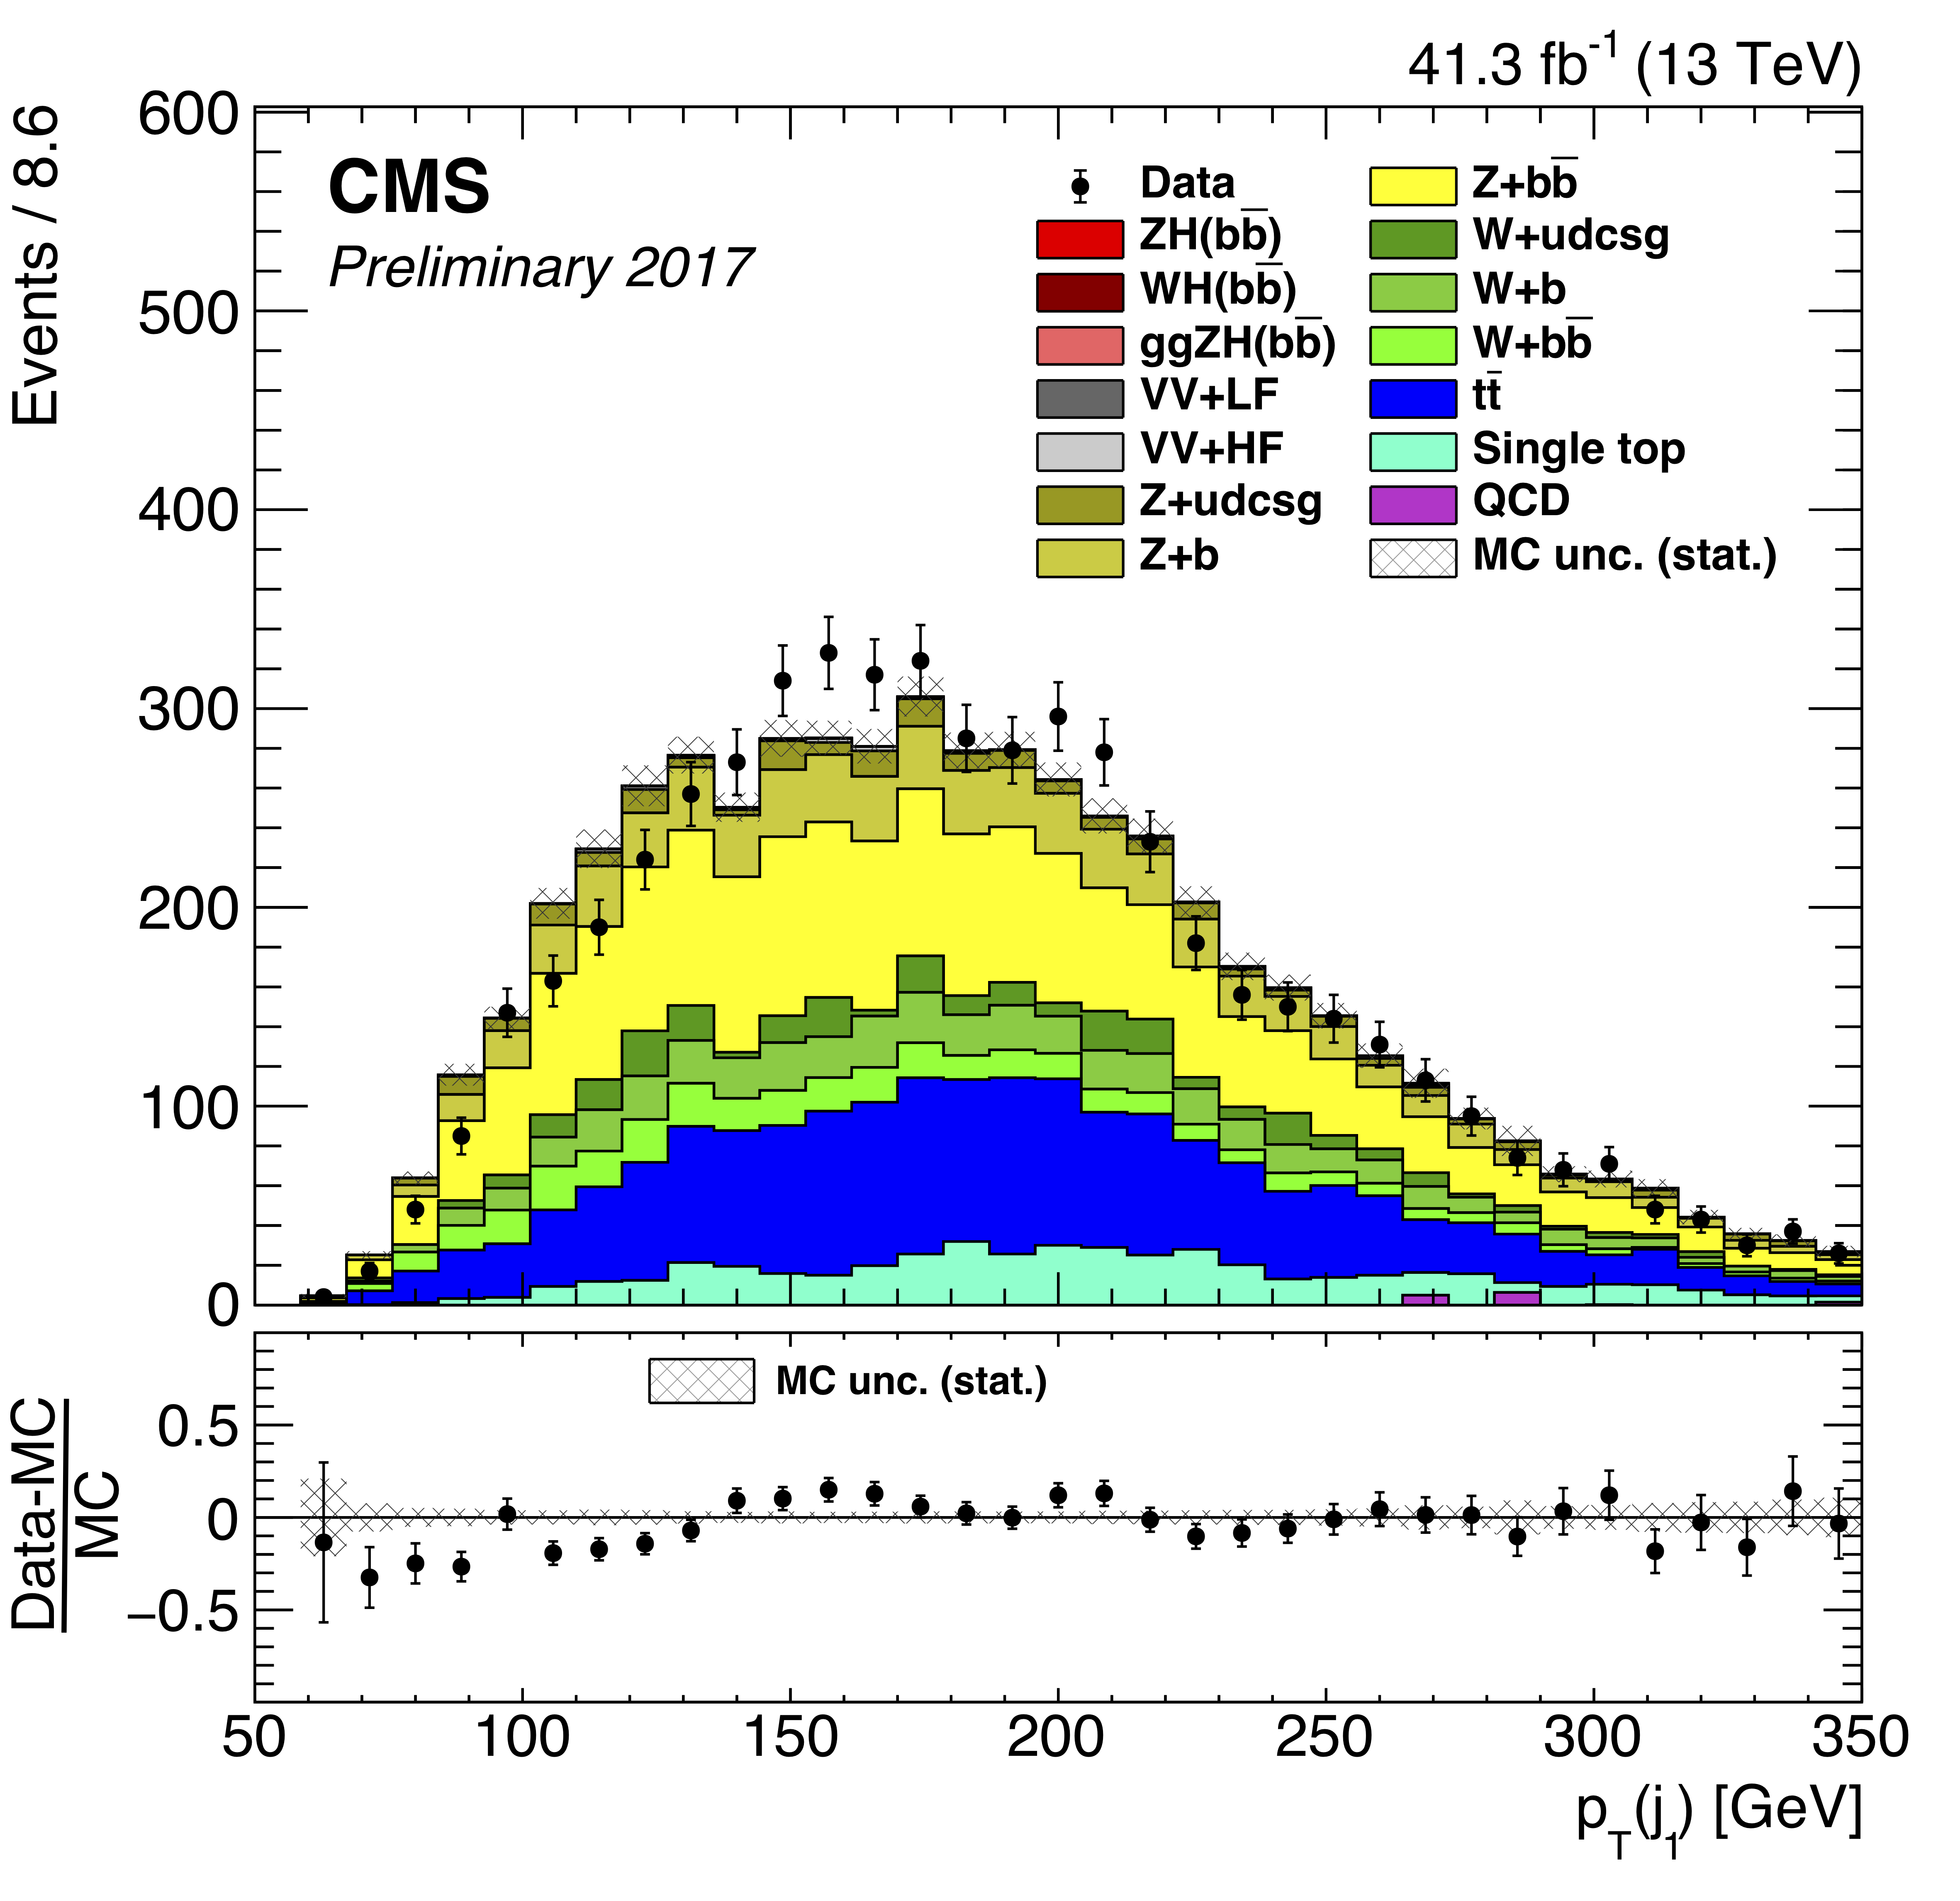
\includegraphics[width=0.39\linewidth]{images/CR_Znn_ZHF/hJets_leadingPt}}
    \subfigure [] {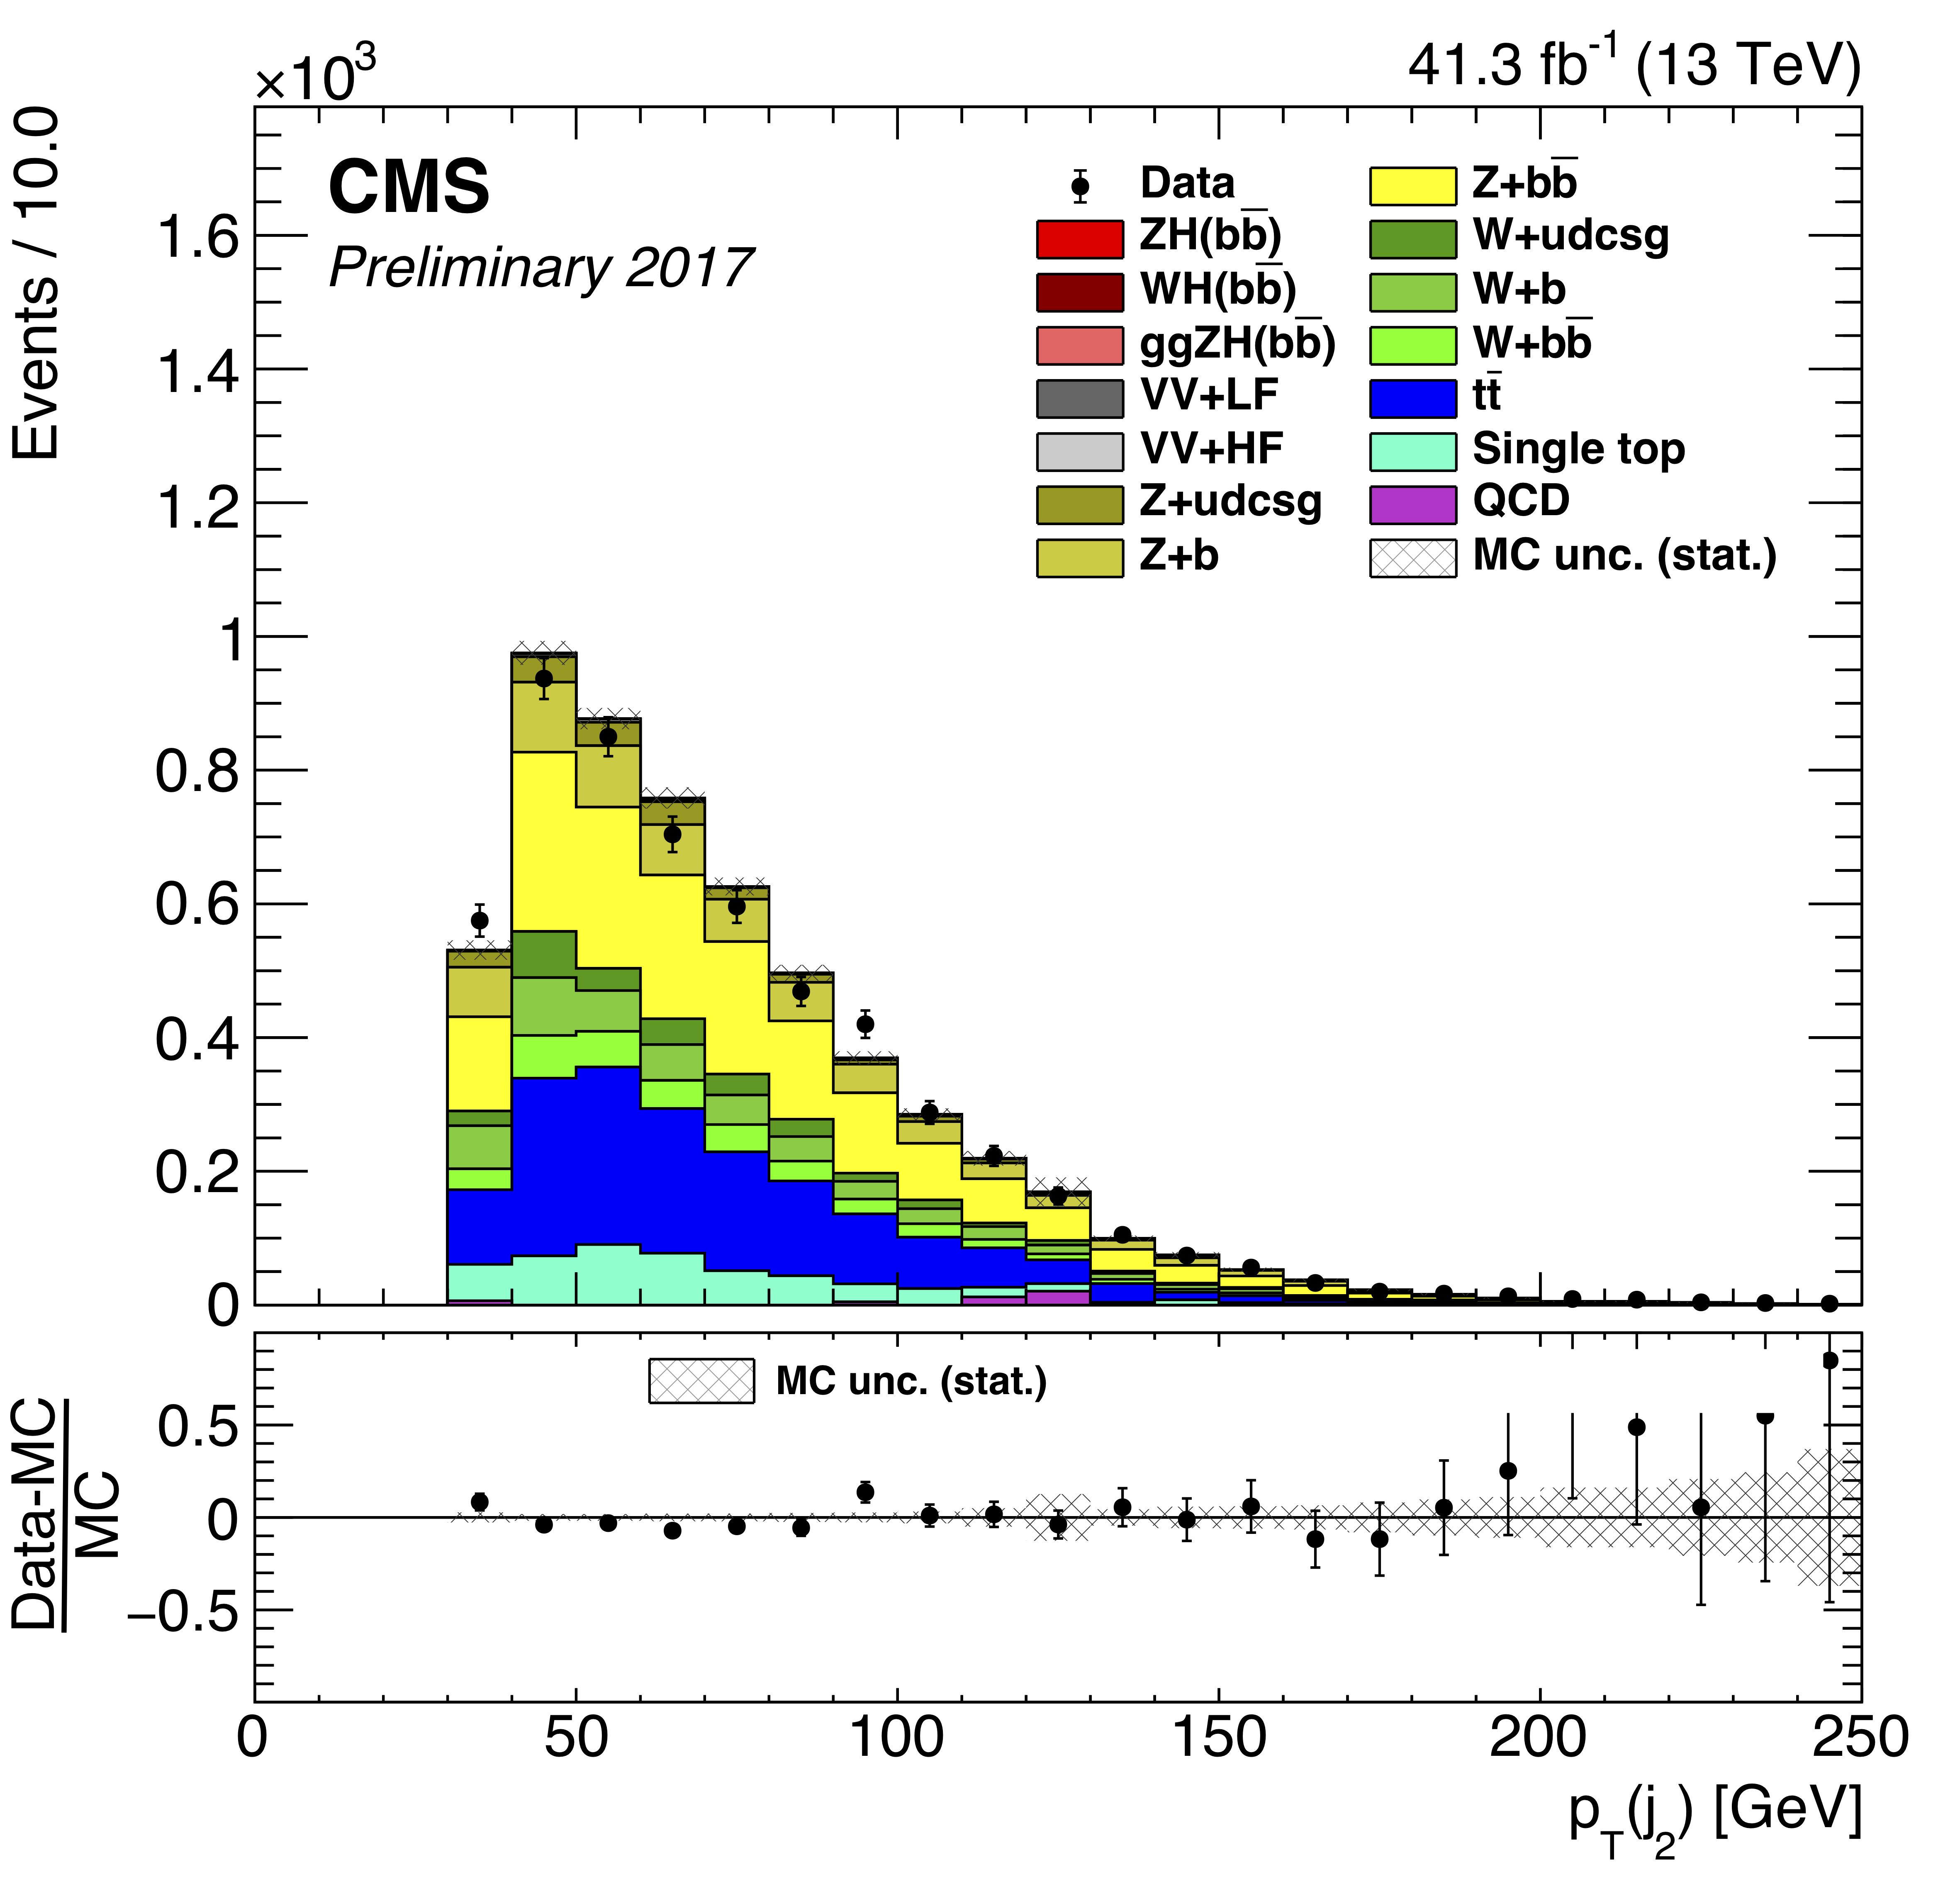
\includegraphics[width=0.39\linewidth]{images/CR_Znn_ZHF/hJets_subleadingPt}}
  }
  \caption[\bosZ+heavy Control Region Distributions for the \ZnnH\ Channel]{The distributions of variables in the \bosZ+heavy control region of the \ZnnH\ channel: A) $m(jj)$, B) $\pT(jj)$, C) \btagmax, D) \btagmin, E) \pTjmax, F) \pTjmin.}
  \label{fig:CR_Znn_ZHF_1}
\end{figure}

\clearpage

\begin{figure}[htbp]
  \centering
  \mbox{
    \subfigure [] {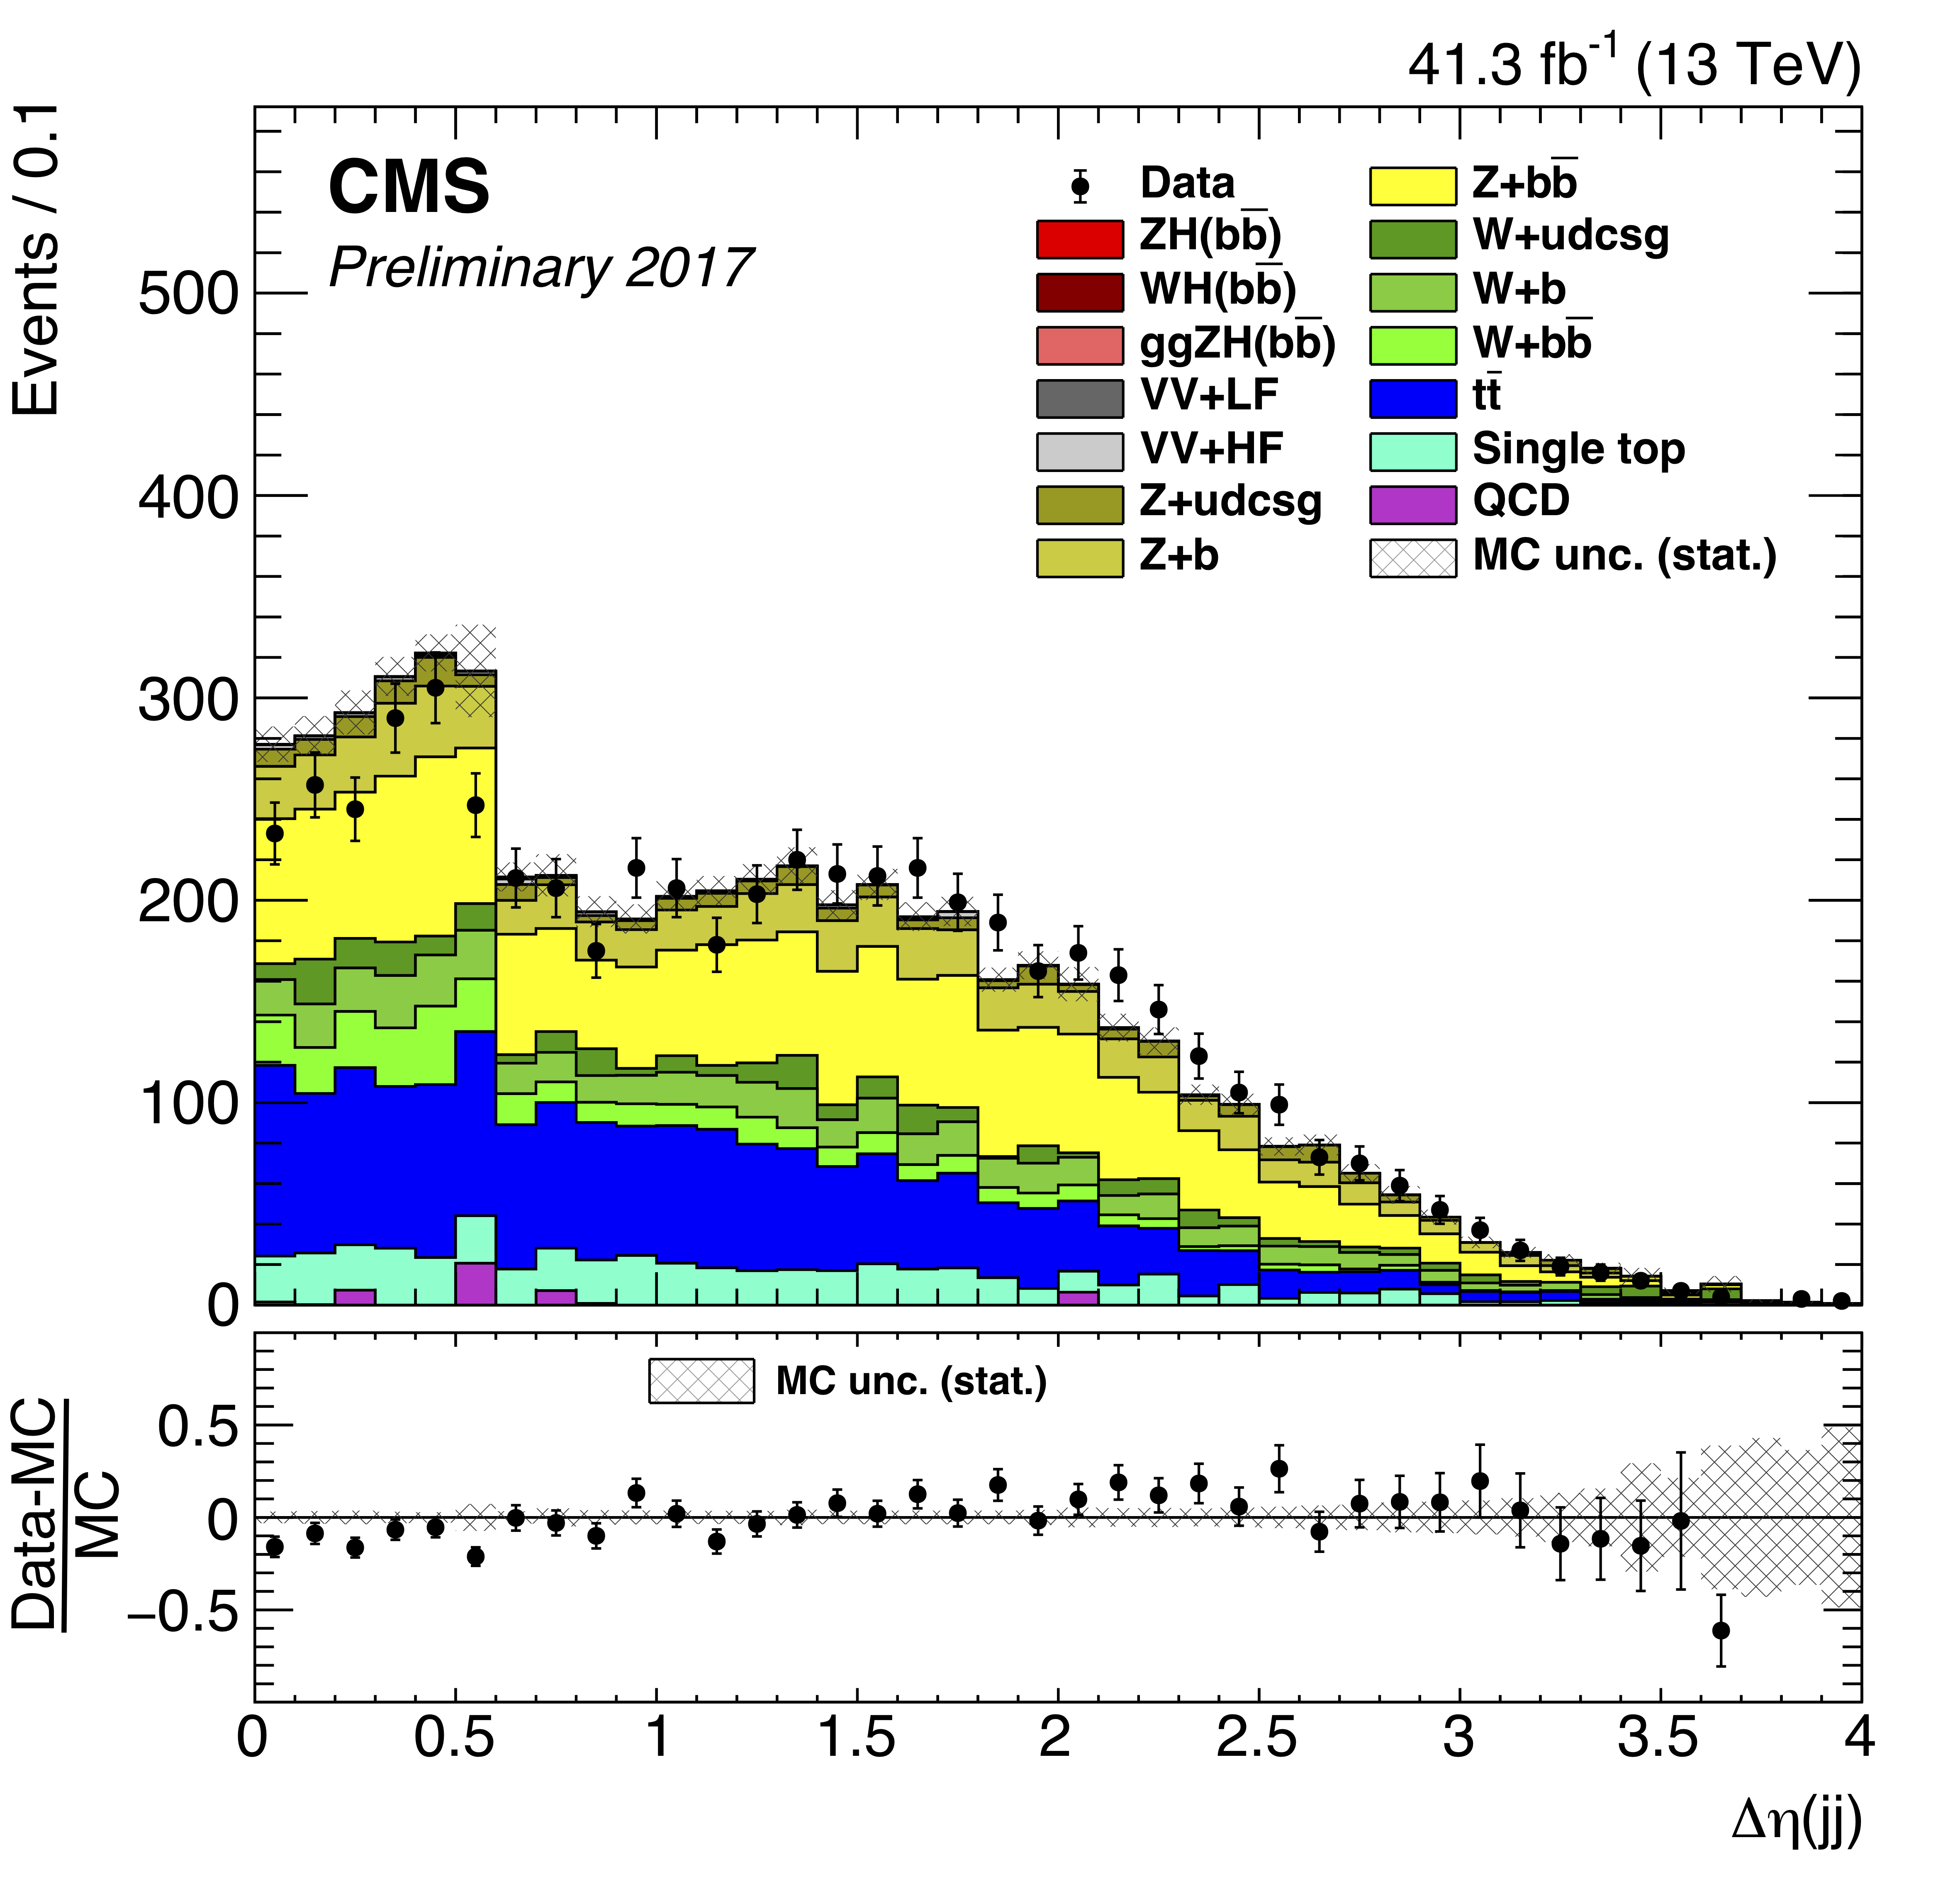
\includegraphics[width=0.39\linewidth]{images/CR_Znn_ZHF/HJ1_HJ2_dEta}}
    \subfigure [] {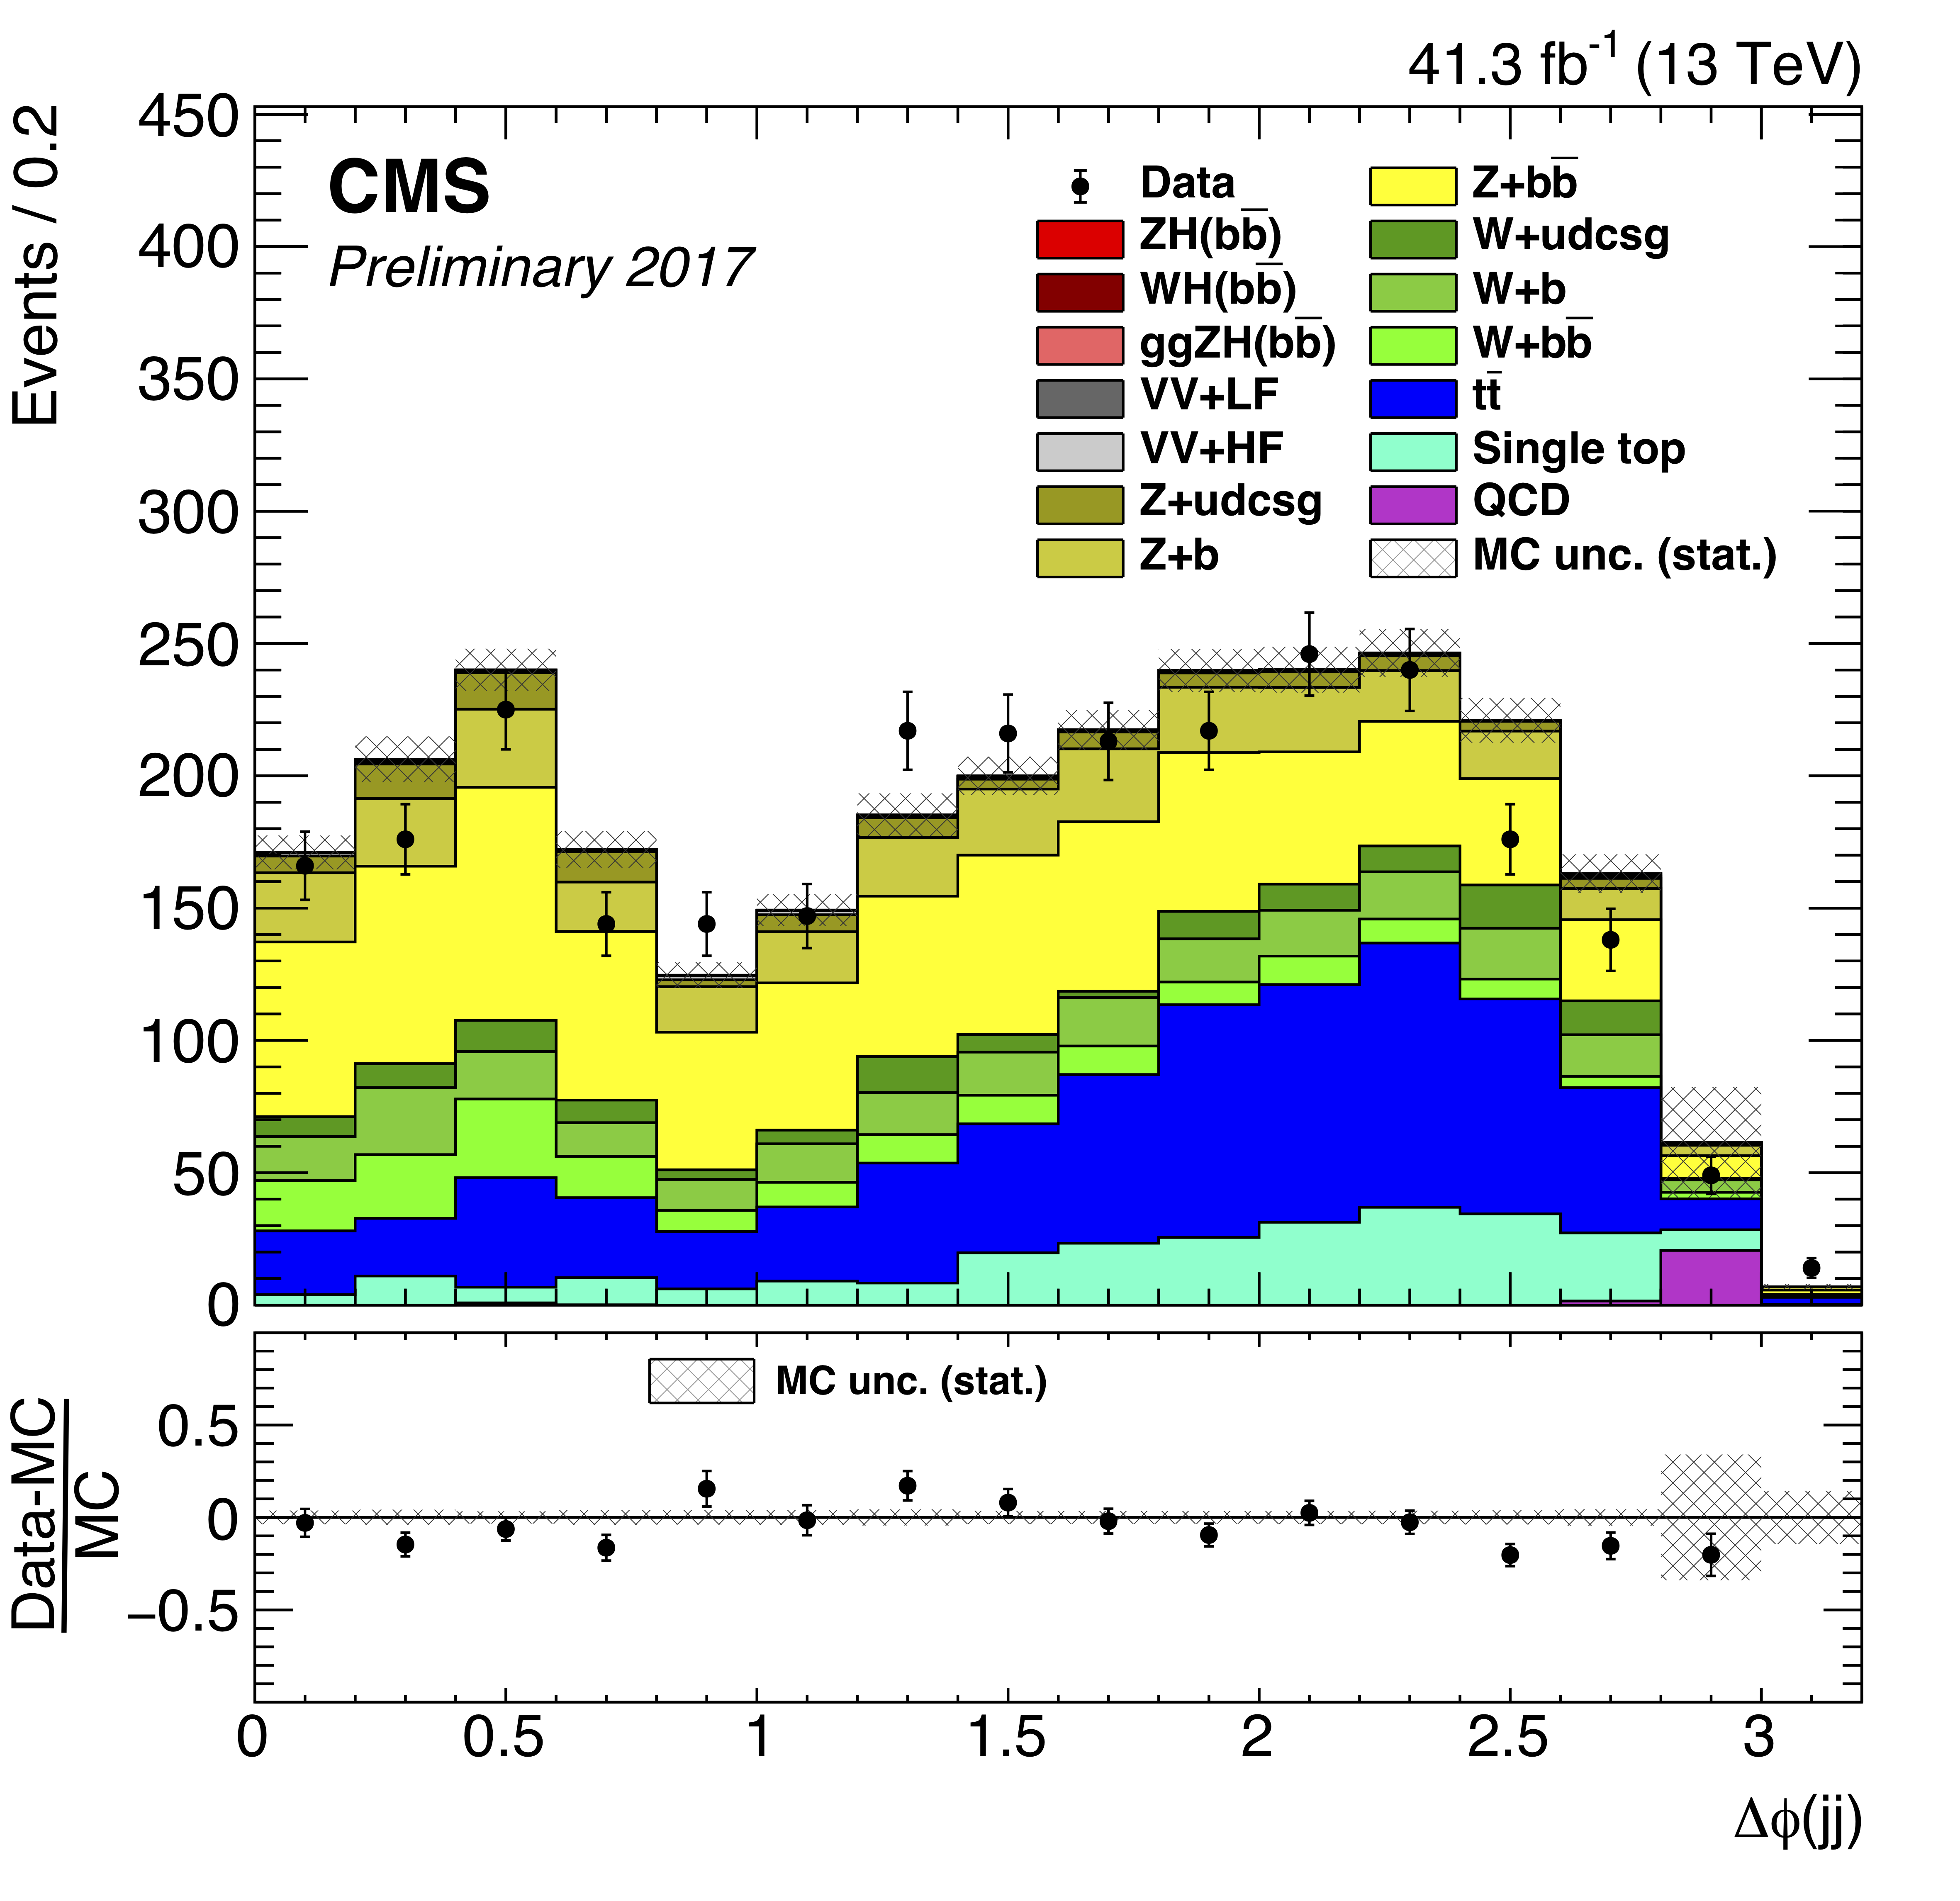
\includegraphics[width=0.39\linewidth]{images/CR_Znn_ZHF/HJ1_HJ2_dPhi}}
  }
  \mbox{
    \subfigure [] {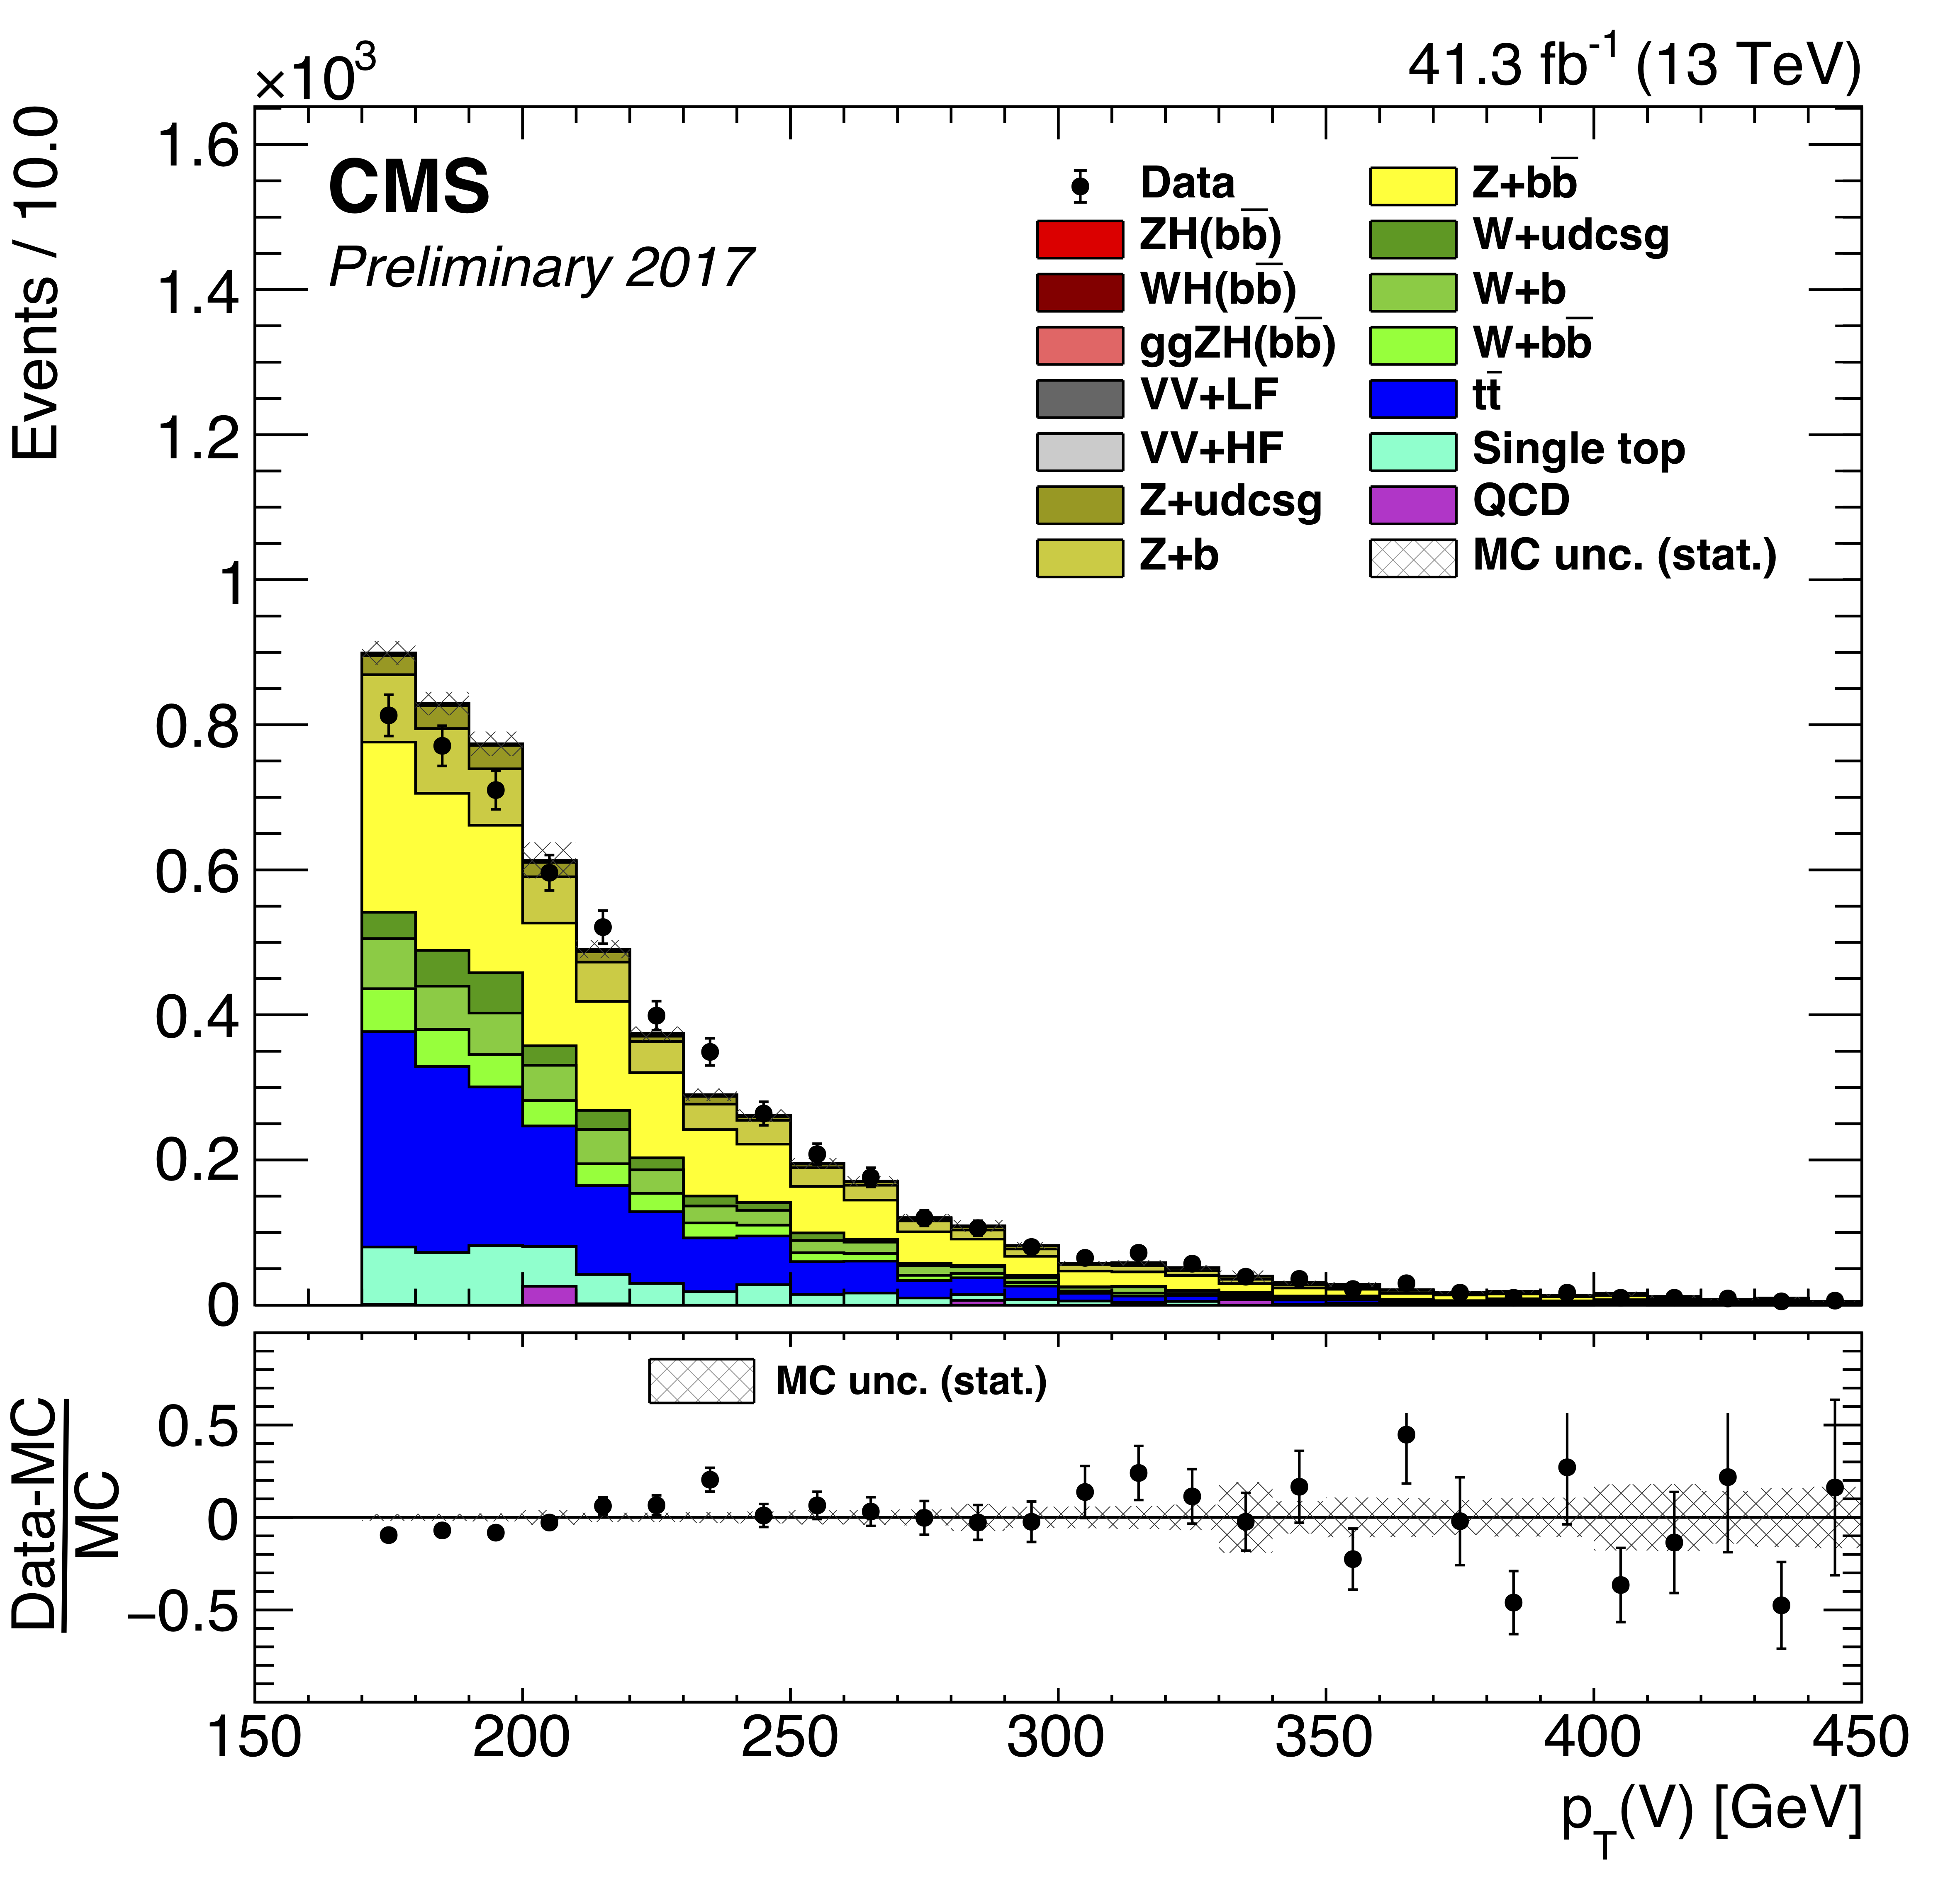
\includegraphics[width=0.39\linewidth]{images/CR_Znn_ZHF/V_pt}}
    \subfigure [] {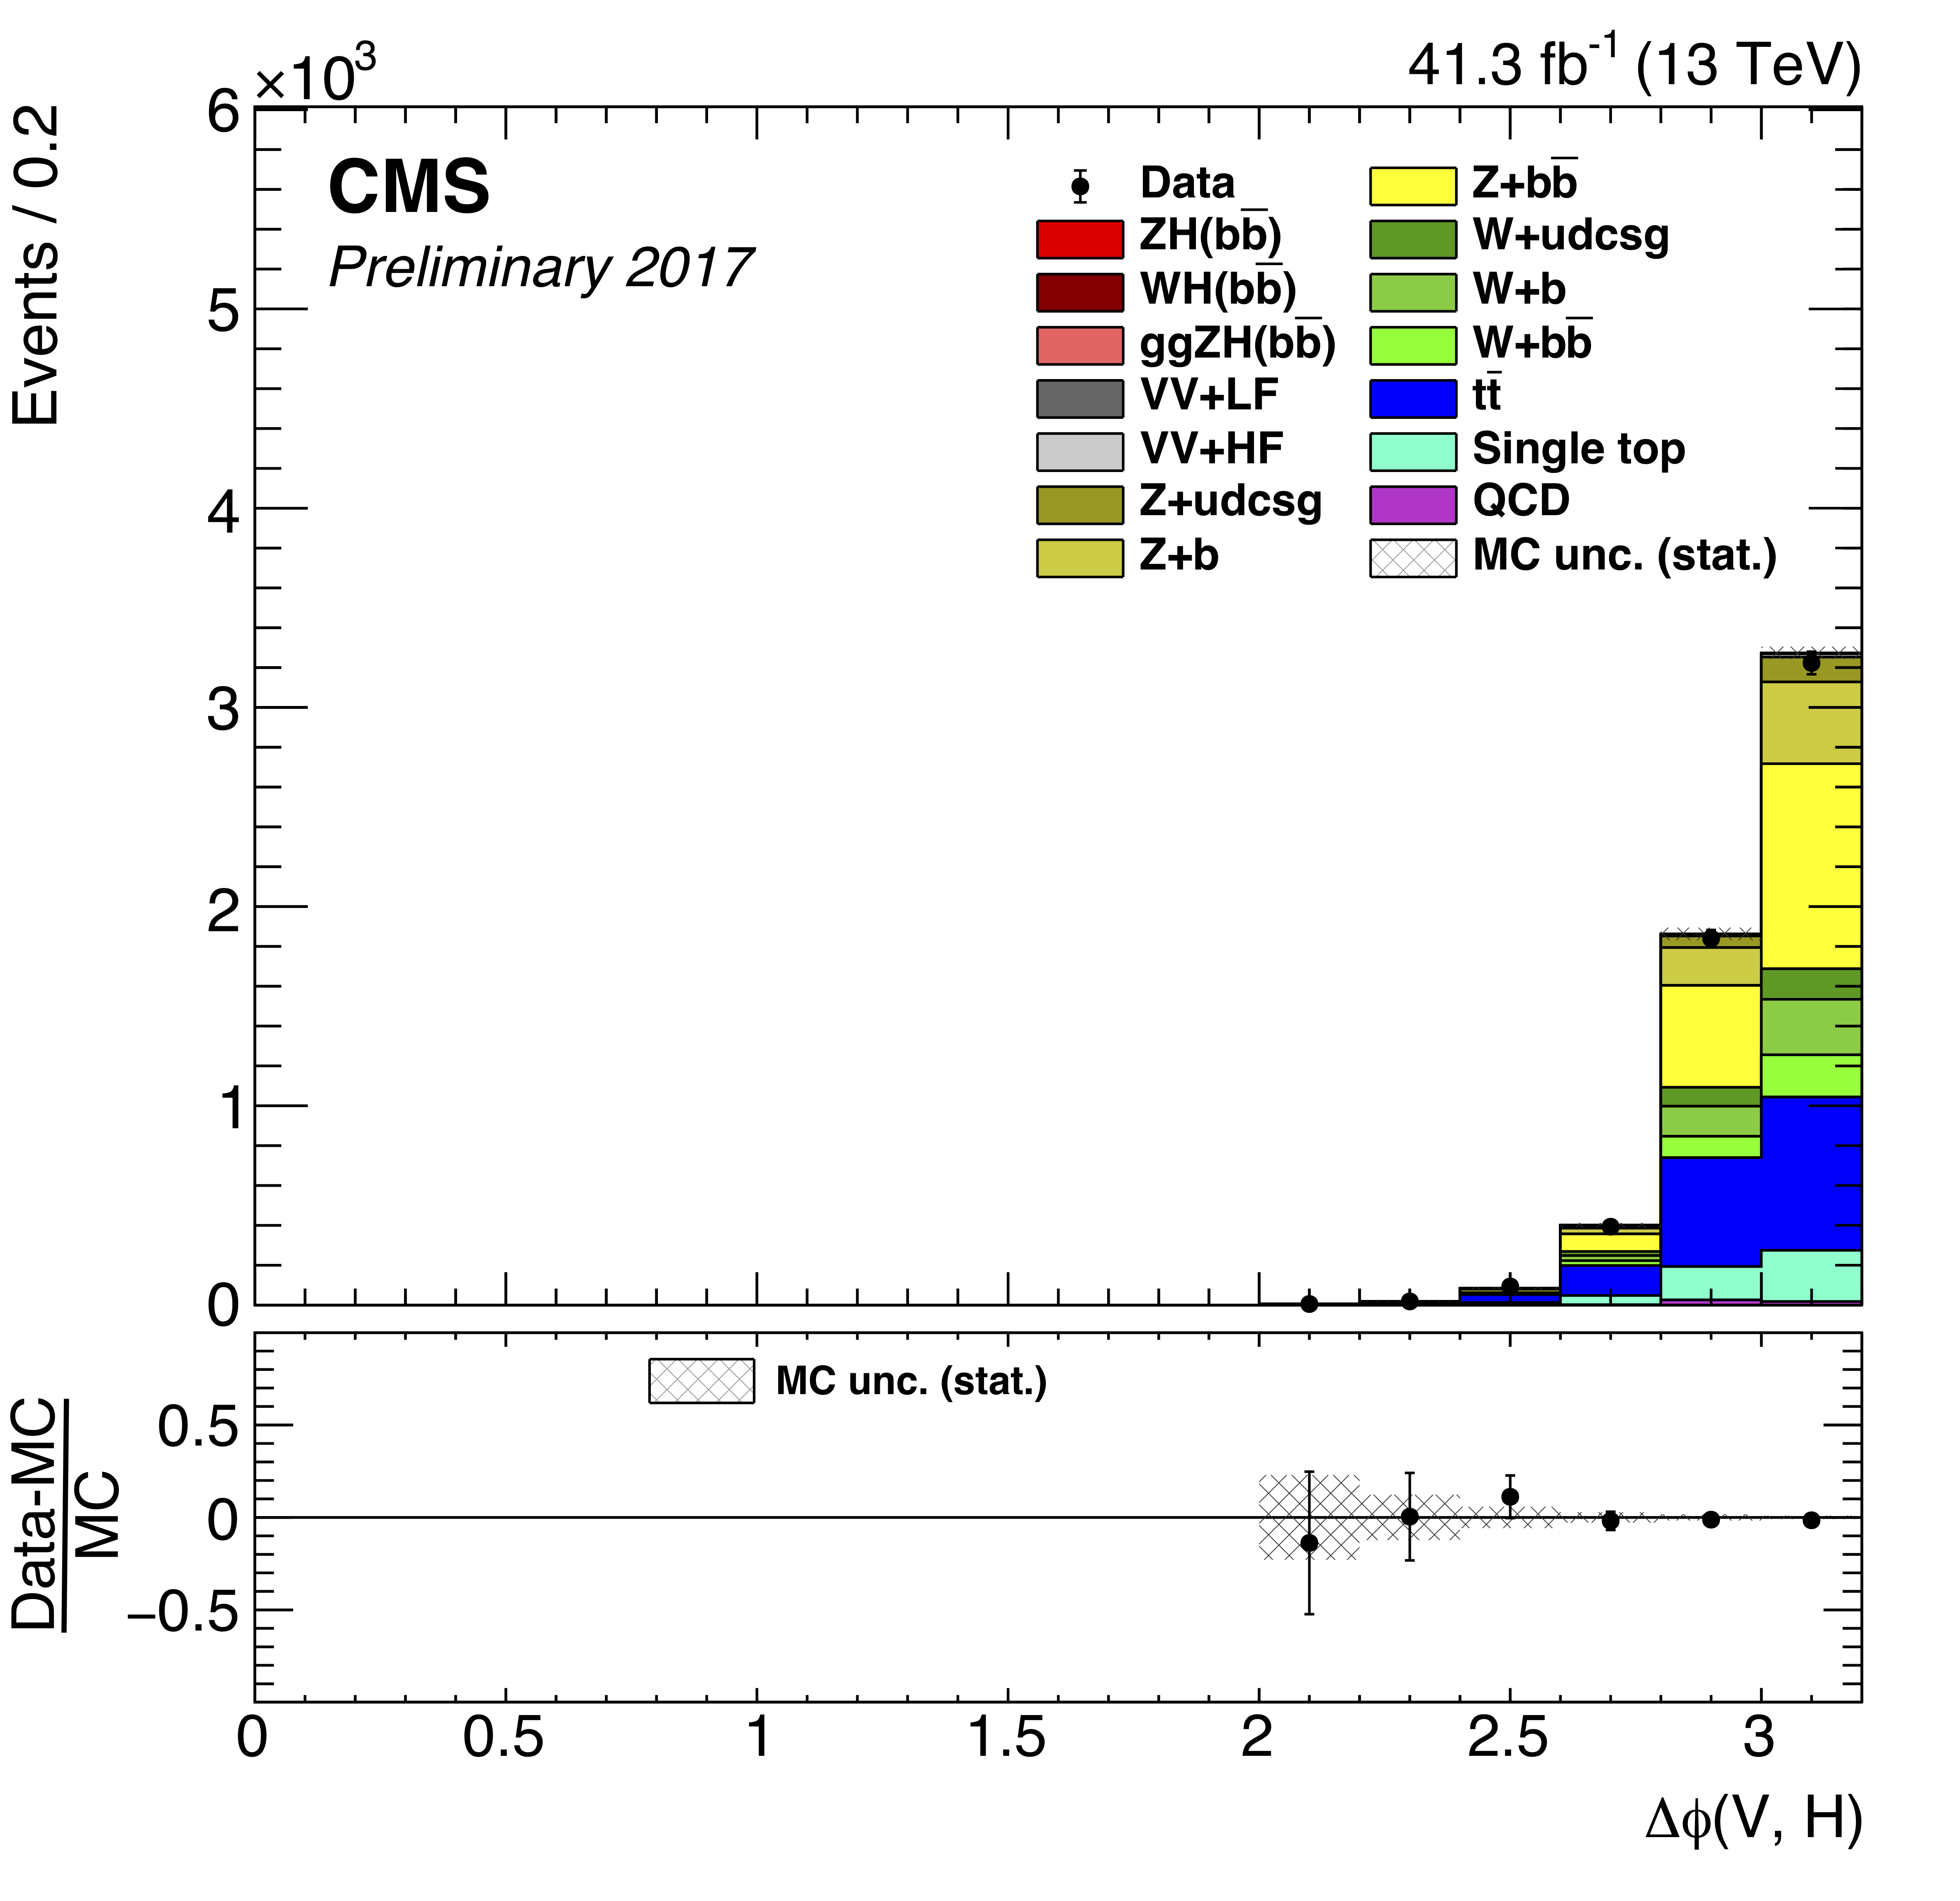
\includegraphics[width=0.39\linewidth]{images/CR_Znn_ZHF/HVdPhi}}
  }
  \mbox{
    \subfigure [] {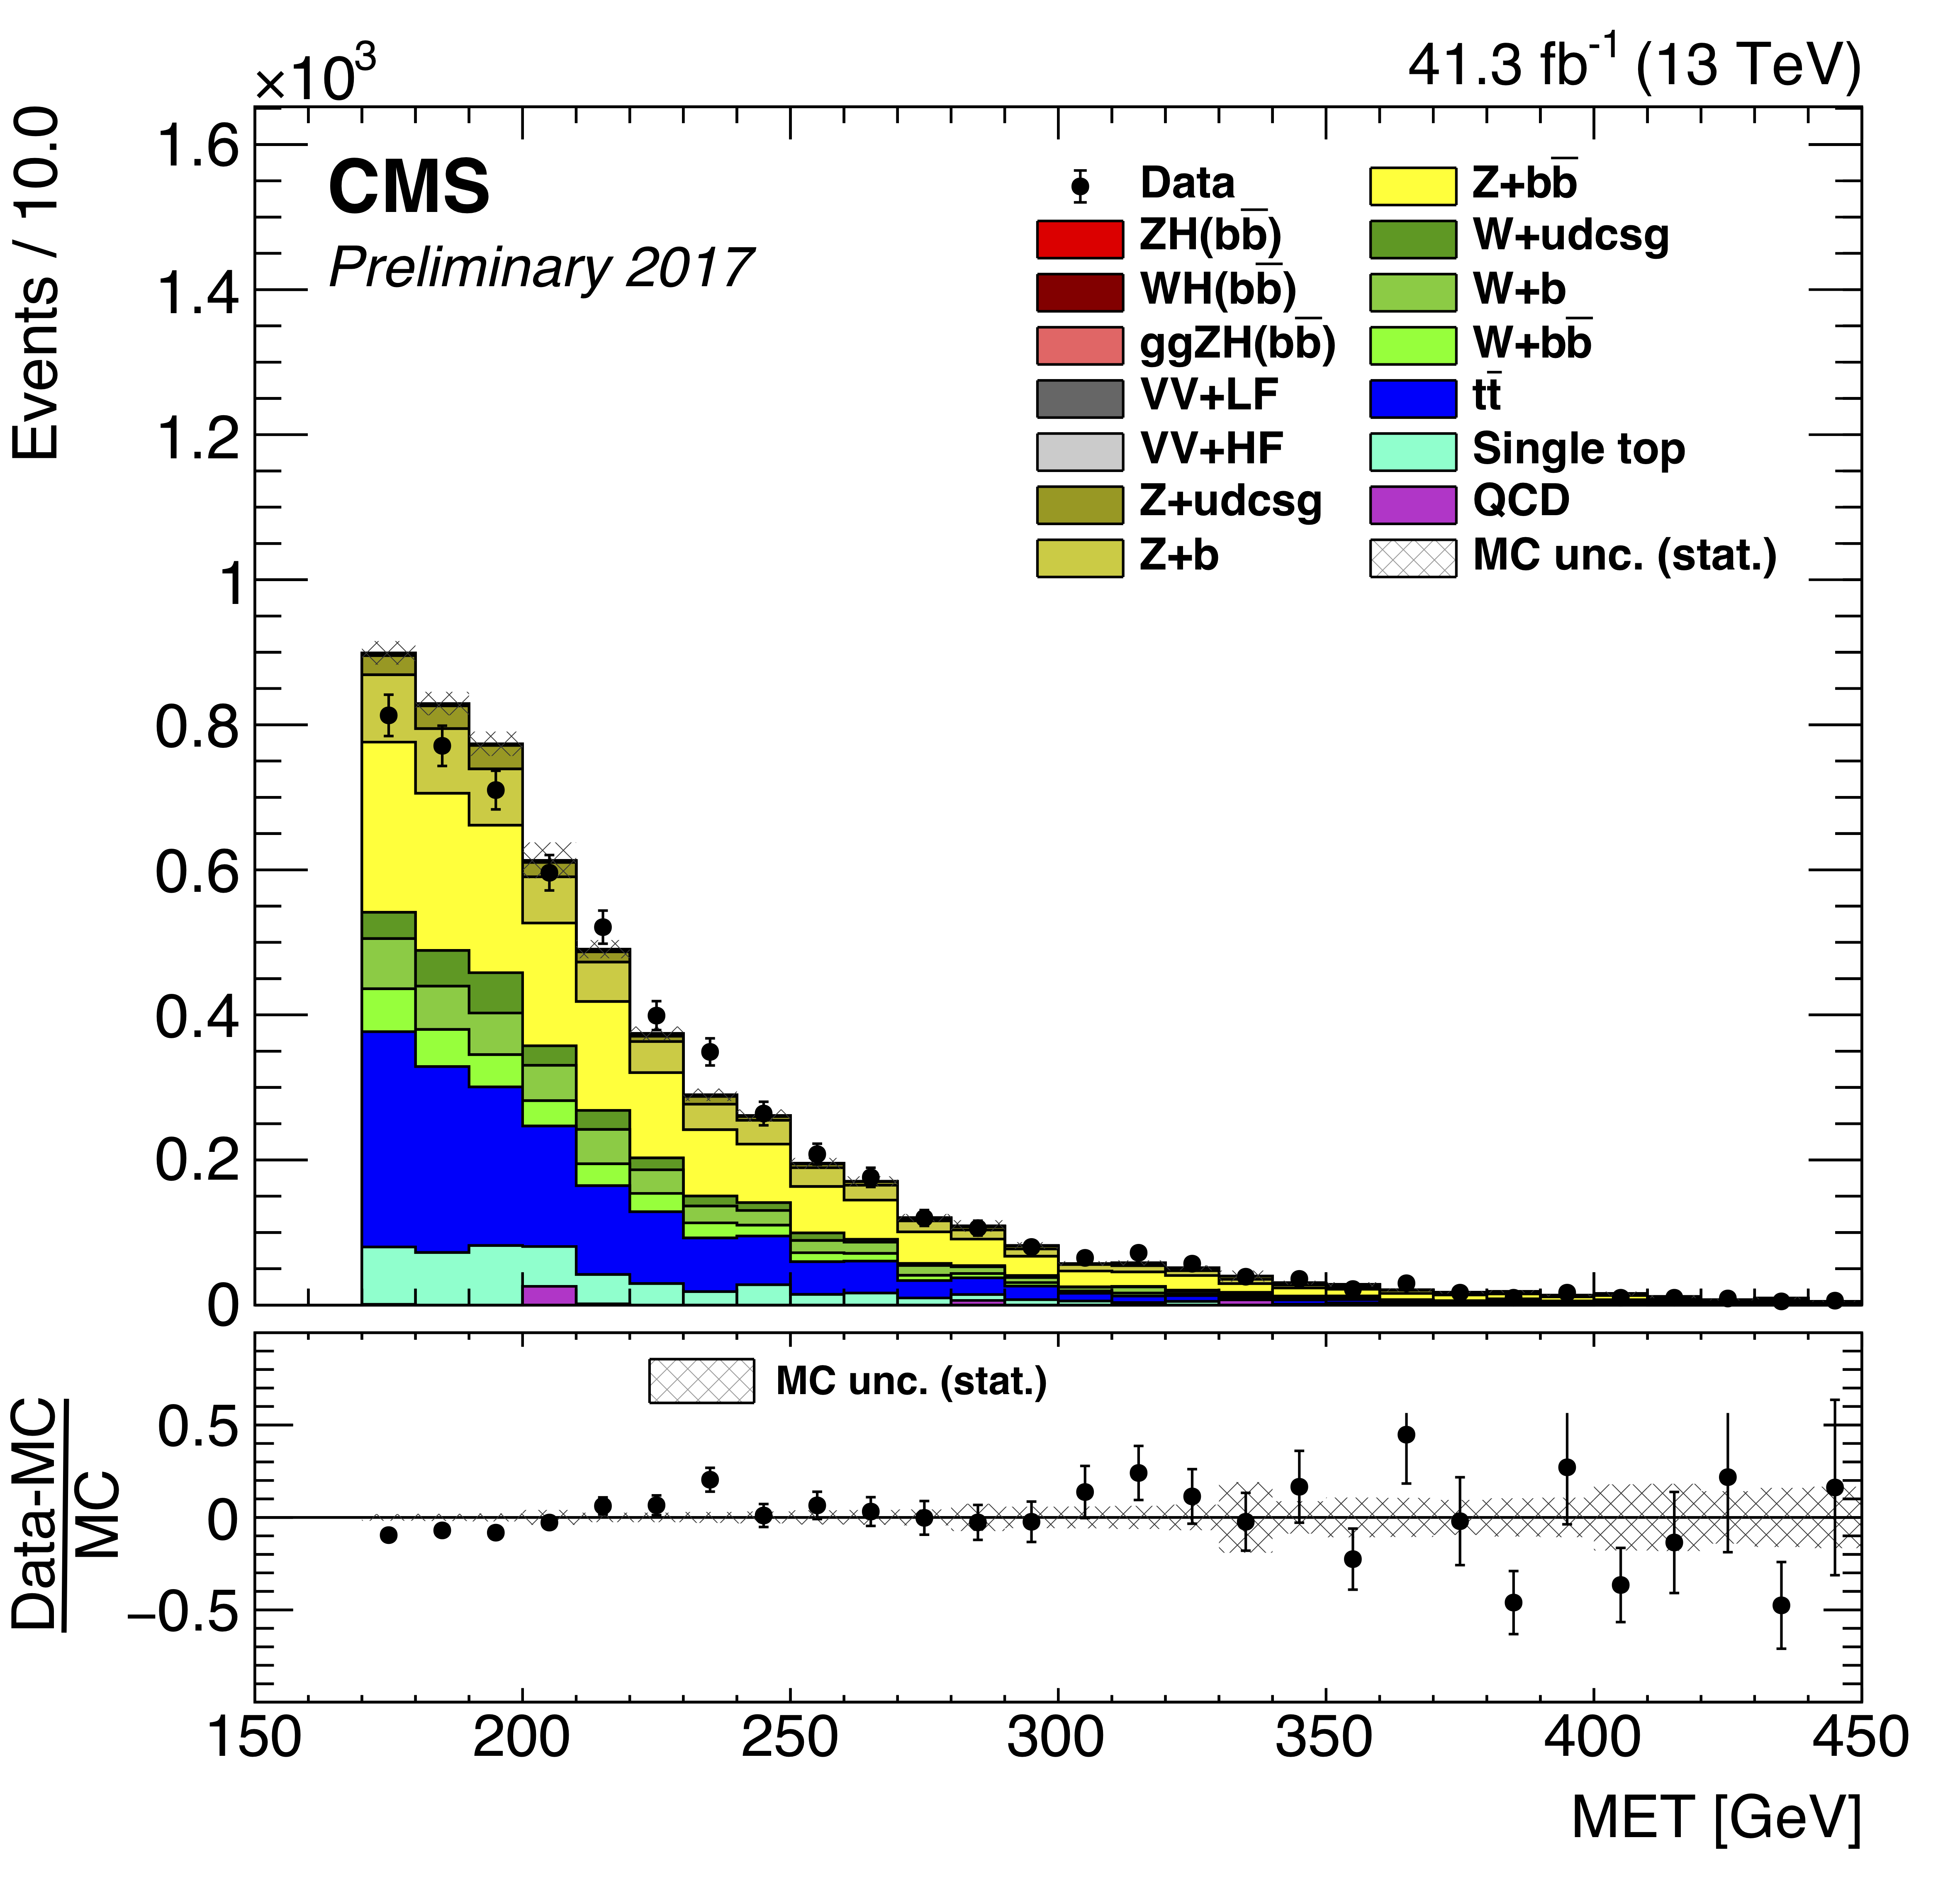
\includegraphics[width=0.39\linewidth]{images/CR_Znn_ZHF/MET_Pt}}
    \subfigure [] {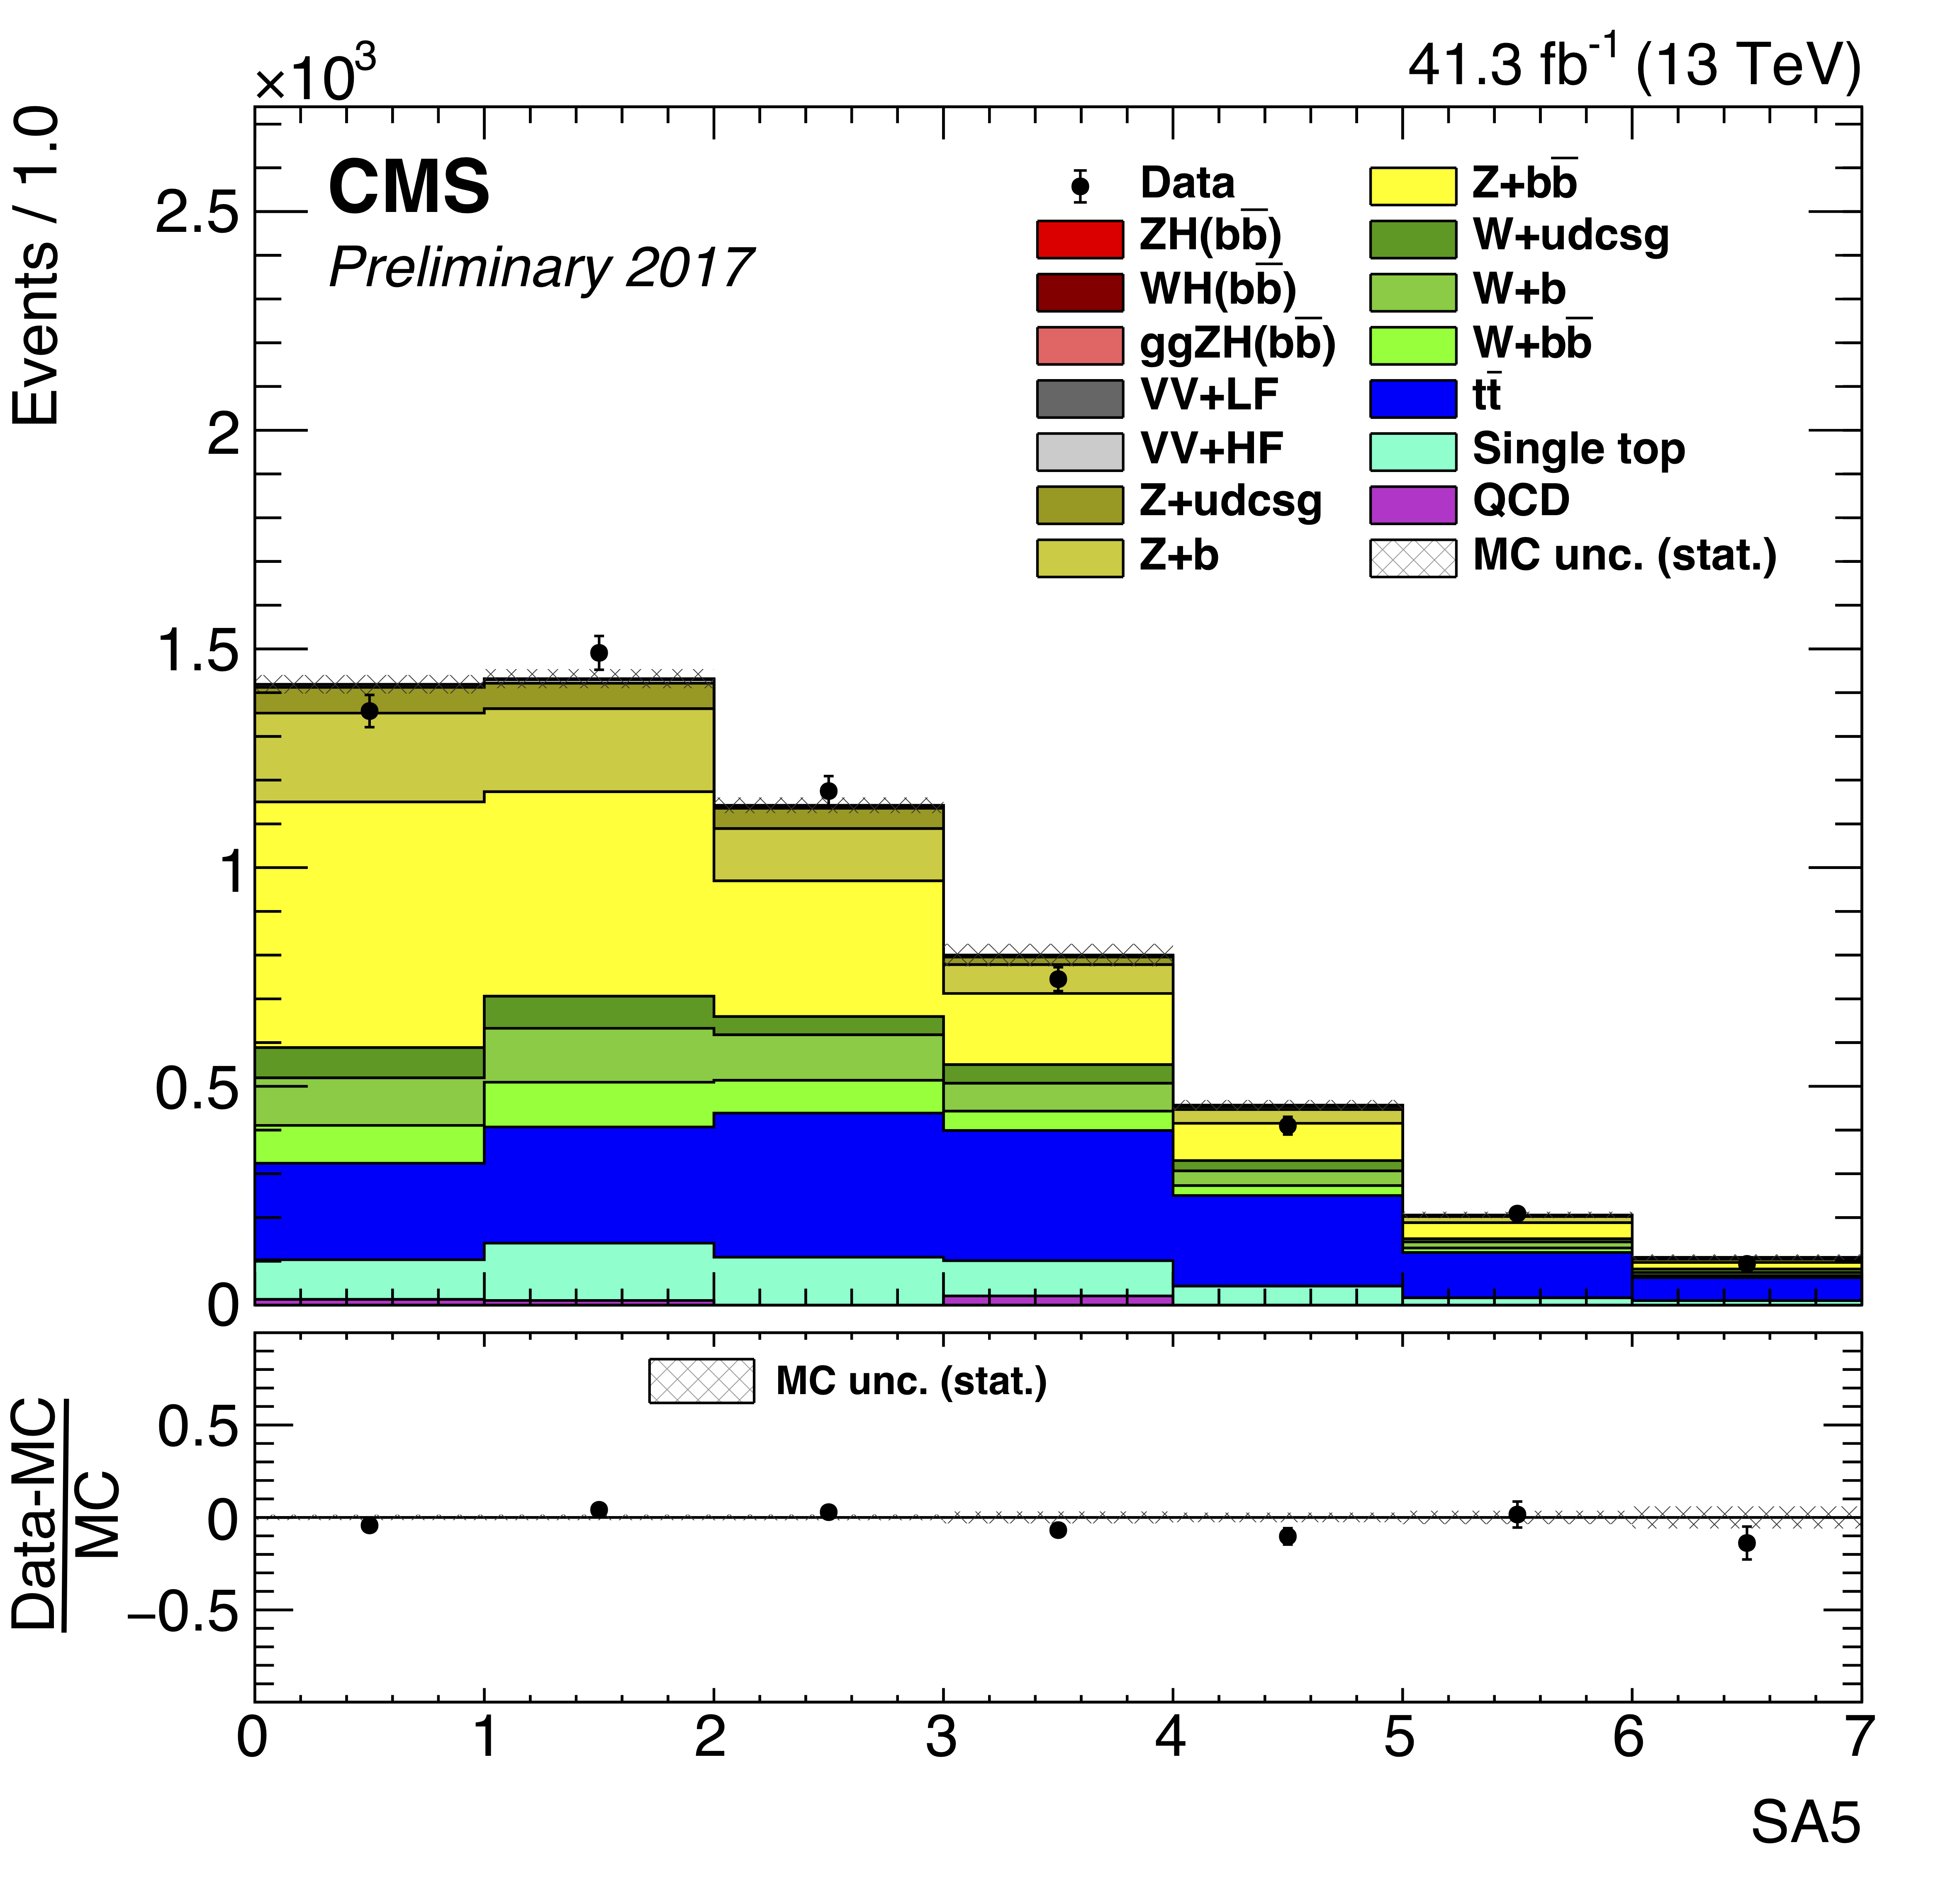
\includegraphics[width=0.39\linewidth]{images/CR_Znn_ZHF/SA5}}
  }
  \caption[Additional \bosZ+heavy Control Region Distributions for the \ZnnH\ Channel]{The distributions of variables in the \bosZ+heavy control region of the \ZnnH\ channel: A) $\left| \Delta \eta (j_{1}, j_{2}) \right|$, B) $\left| \Delta \phi (j_{1}, j_{2}) \right|$, C) $\pT(\bosV)$, D) $\left| \Delta \phi (\bosV, \bosH) \right|$, E) \pTmiss, F) SA5.}
  \label{fig:CR_Znn_ZHF_2}
\end{figure}

\clearpage

%%%%%%%%%%
% WlnHbb %
%%%%%%%%%%

\begin{figure}[htbp]
  \centering
  \mbox{
    \subfigure [] {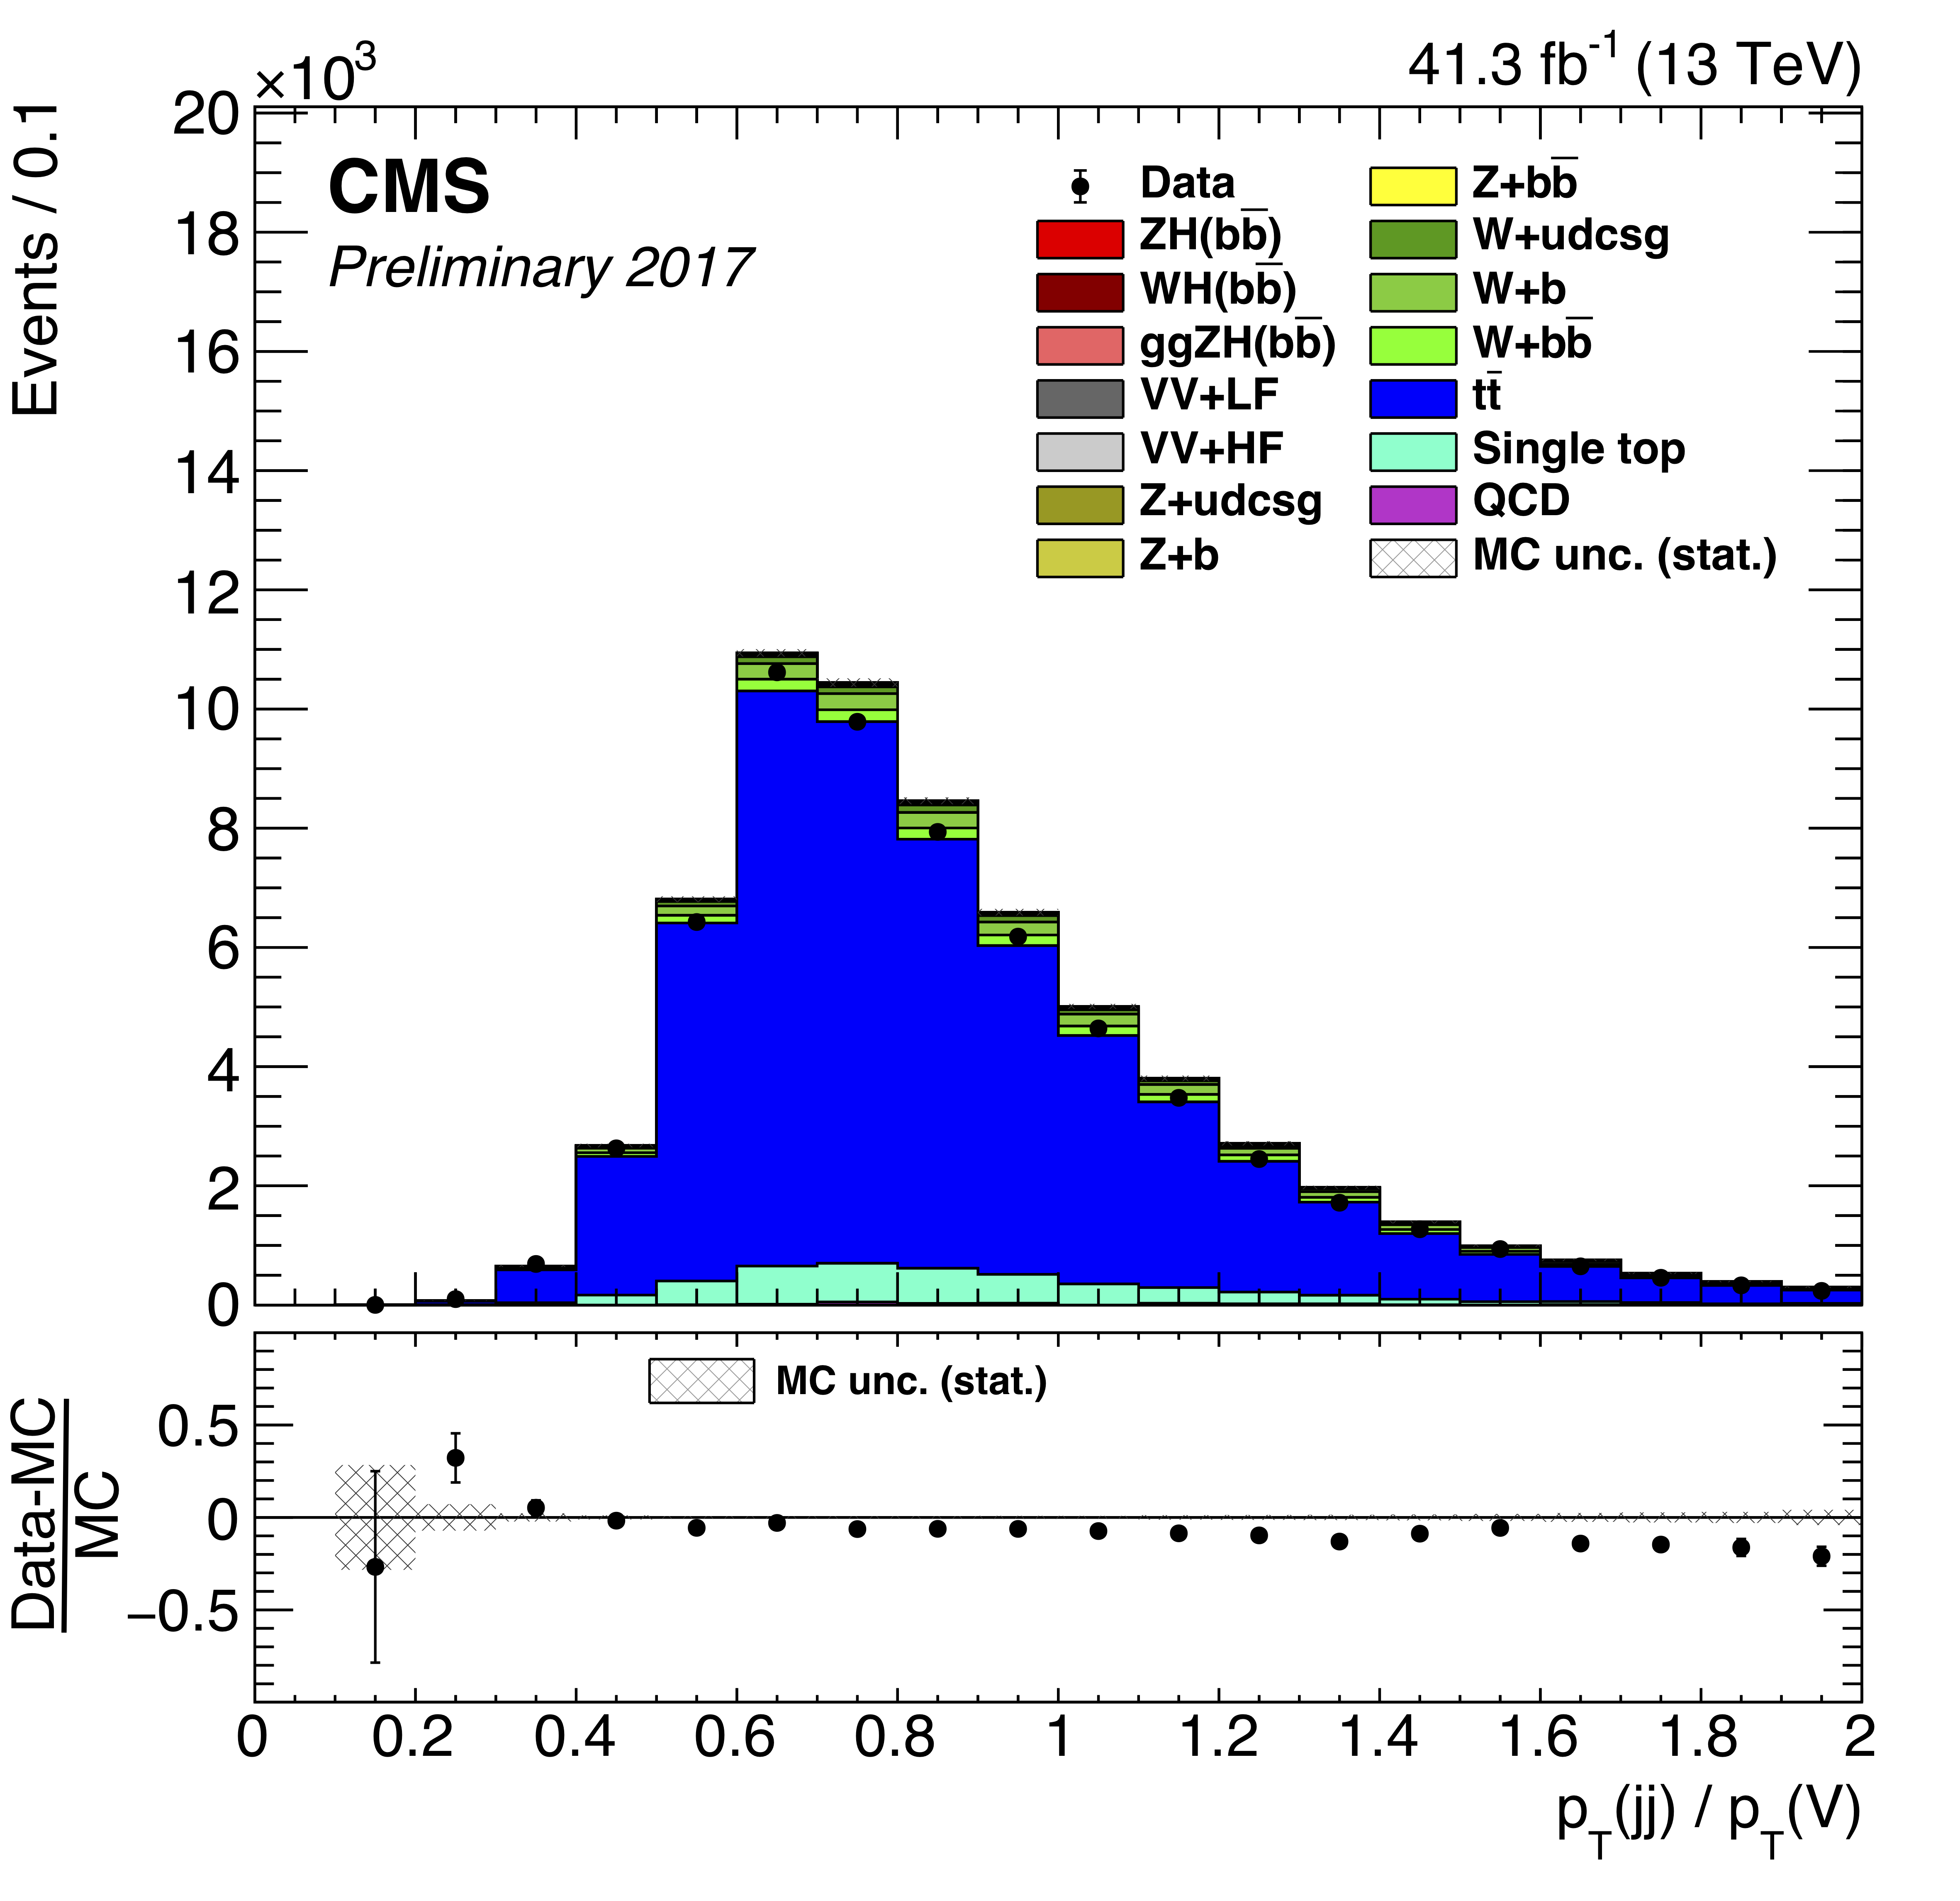
\includegraphics[width=0.39\linewidth]{images/CR_Wen_TT/jjVPtRatio}}
    \subfigure [] {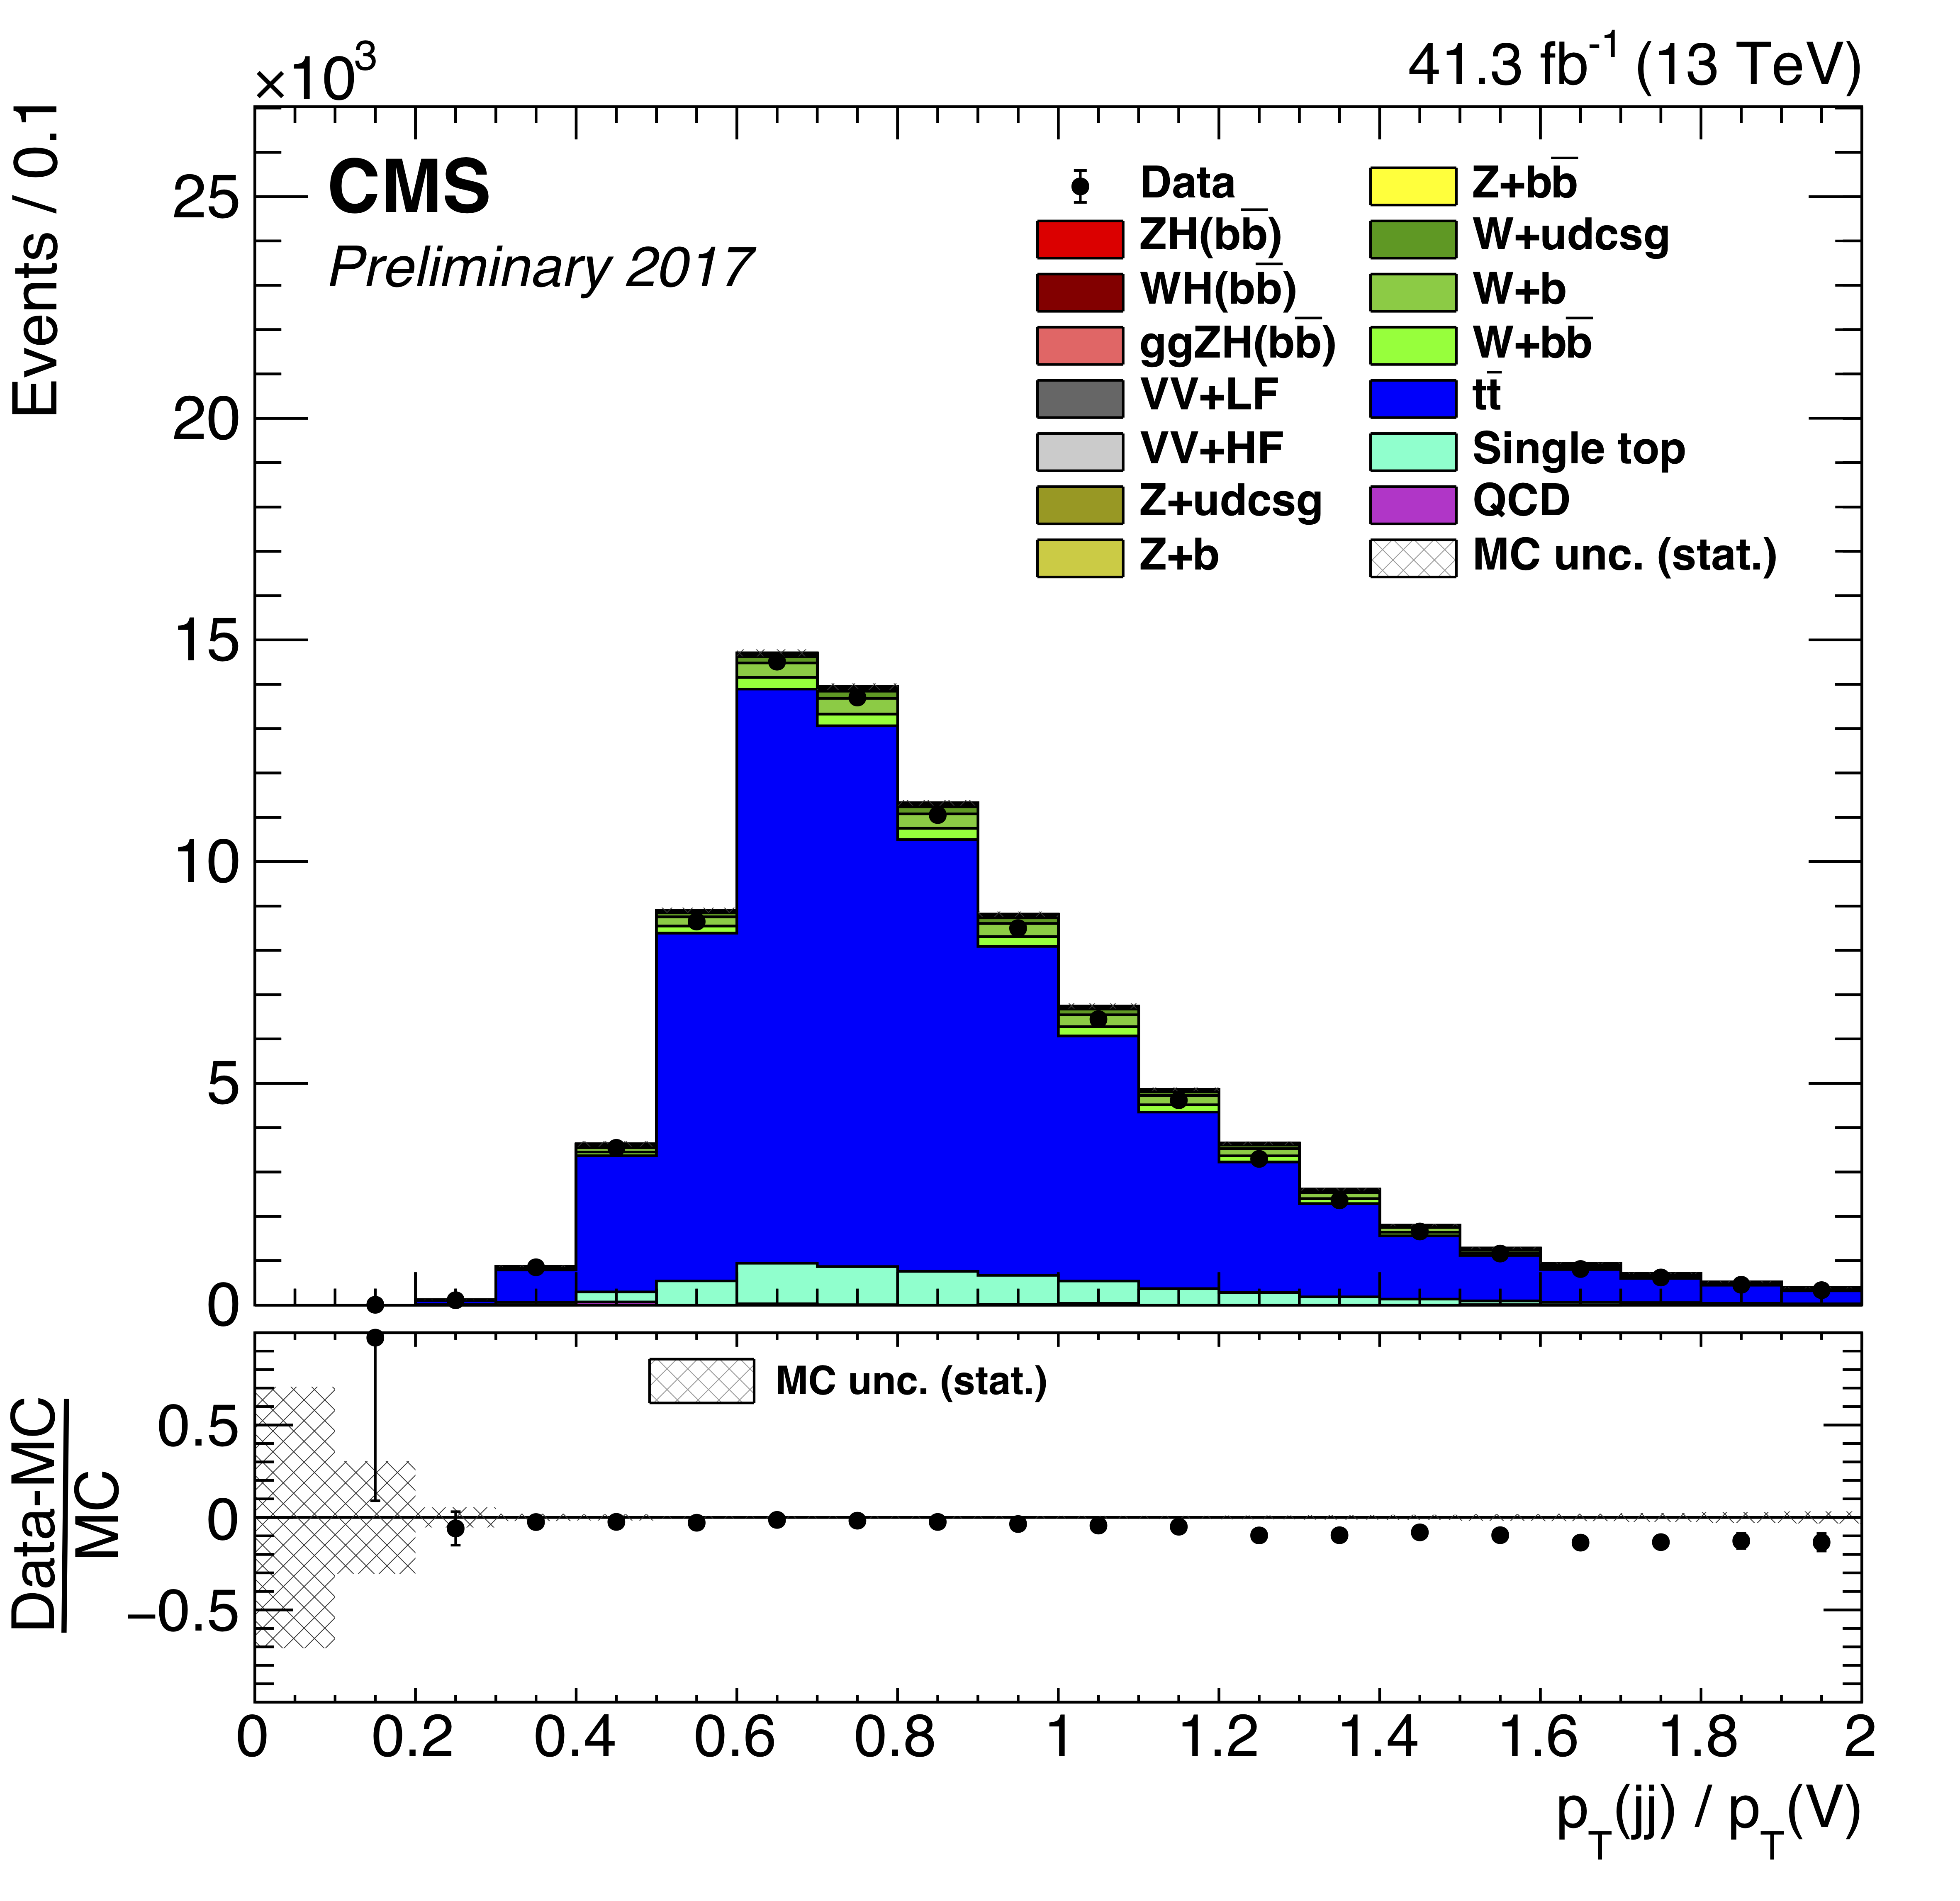
\includegraphics[width=0.39\linewidth]{images/CR_Wmn_TT/jjVPtRatio}}
  }
  \mbox{
    \subfigure [] {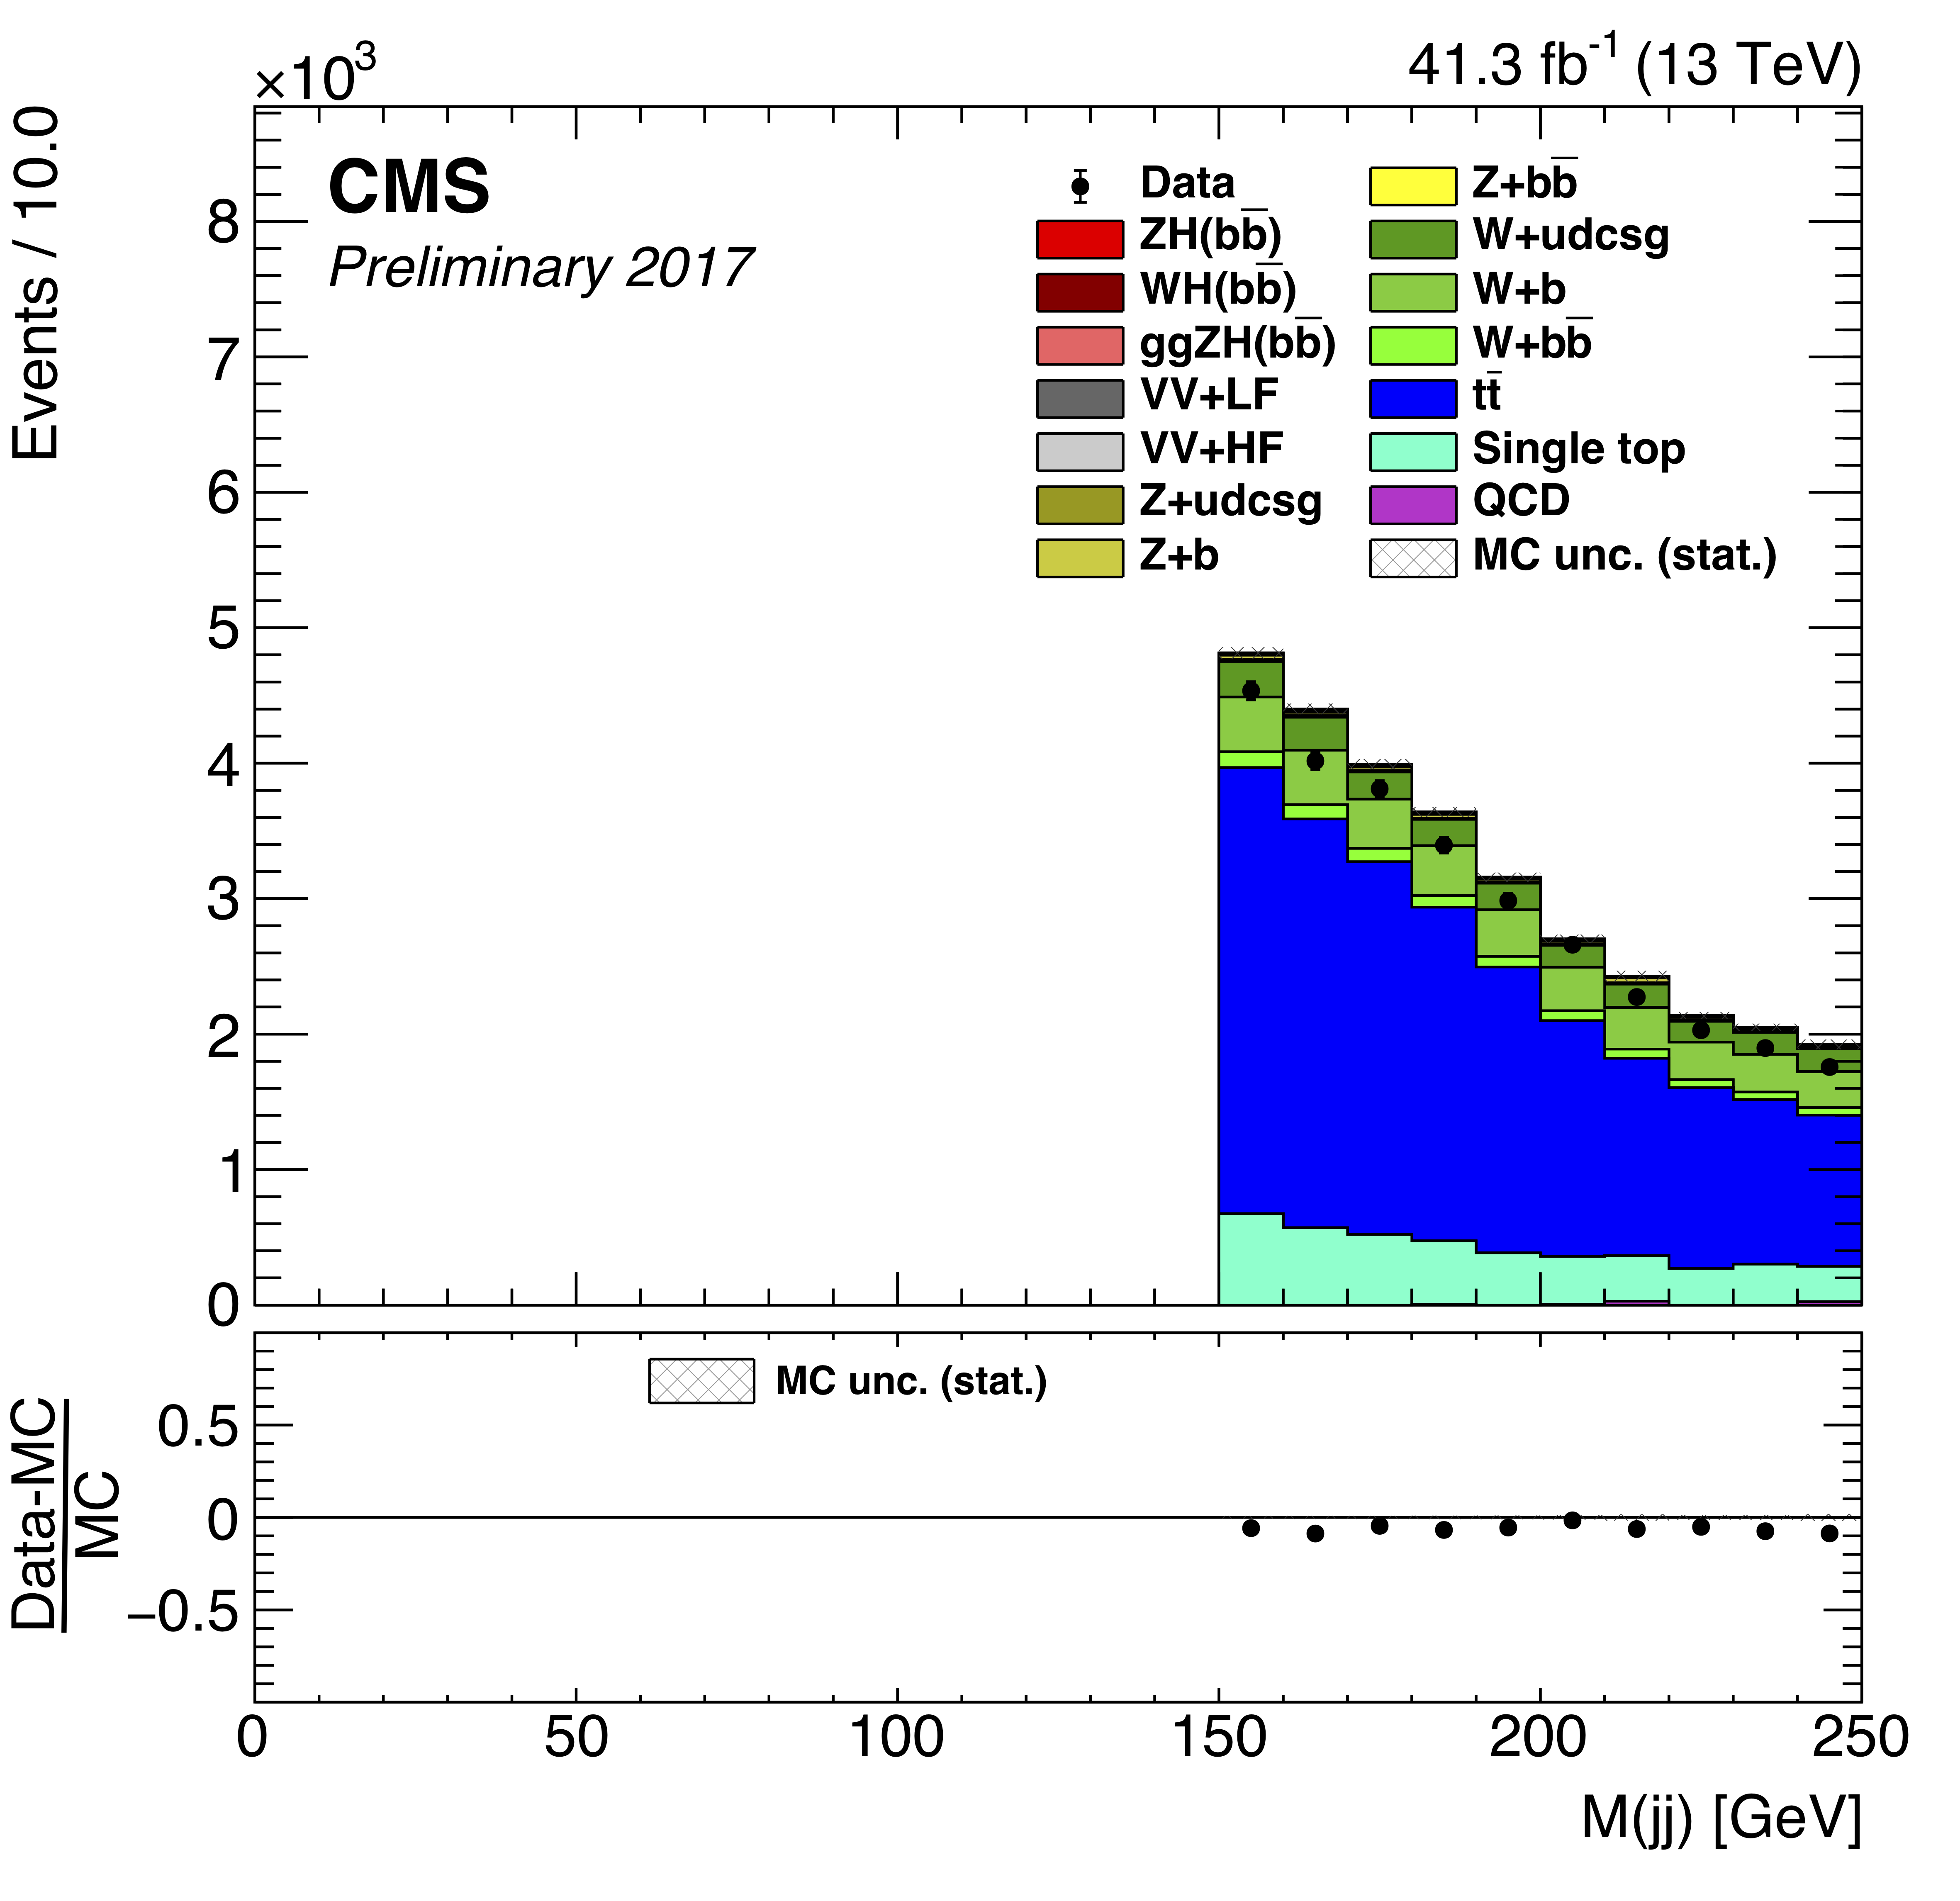
\includegraphics[width=0.39\linewidth]{images/CR_Wen_WLF/H_mass}}
    \subfigure [] {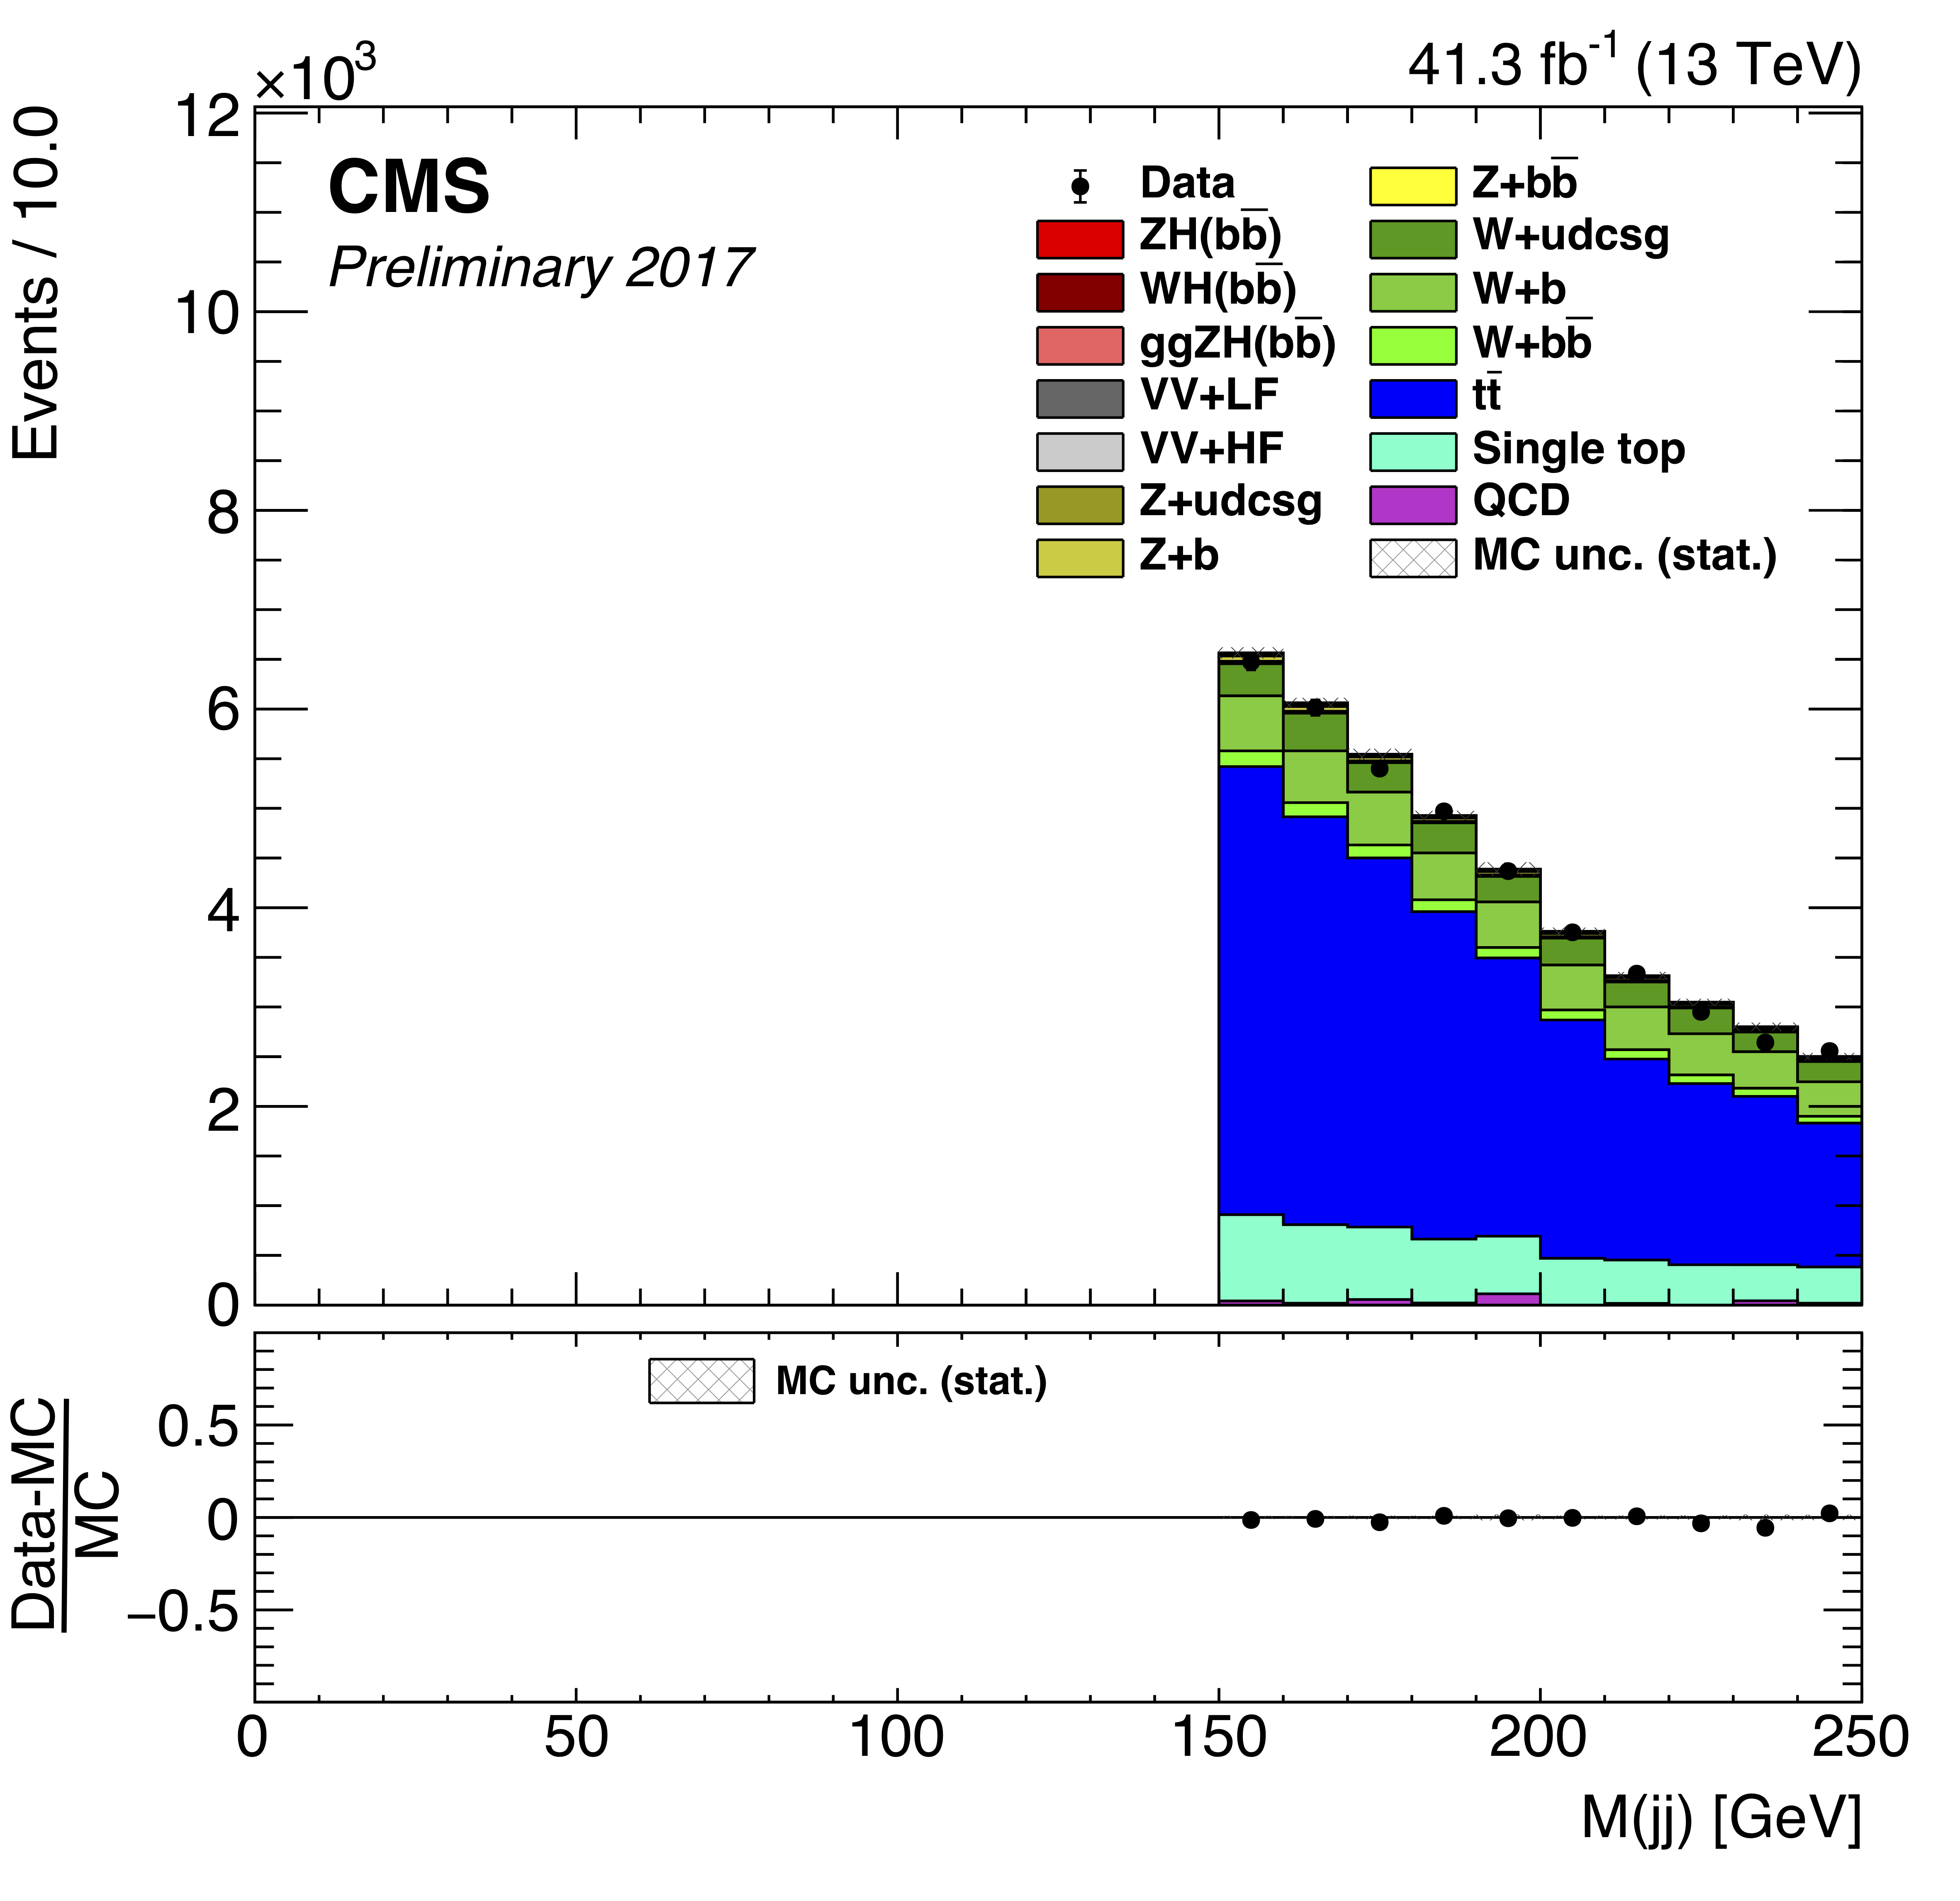
\includegraphics[width=0.39\linewidth]{images/CR_Wmn_WLF/H_mass}}
  }
  \mbox{
    \subfigure [] {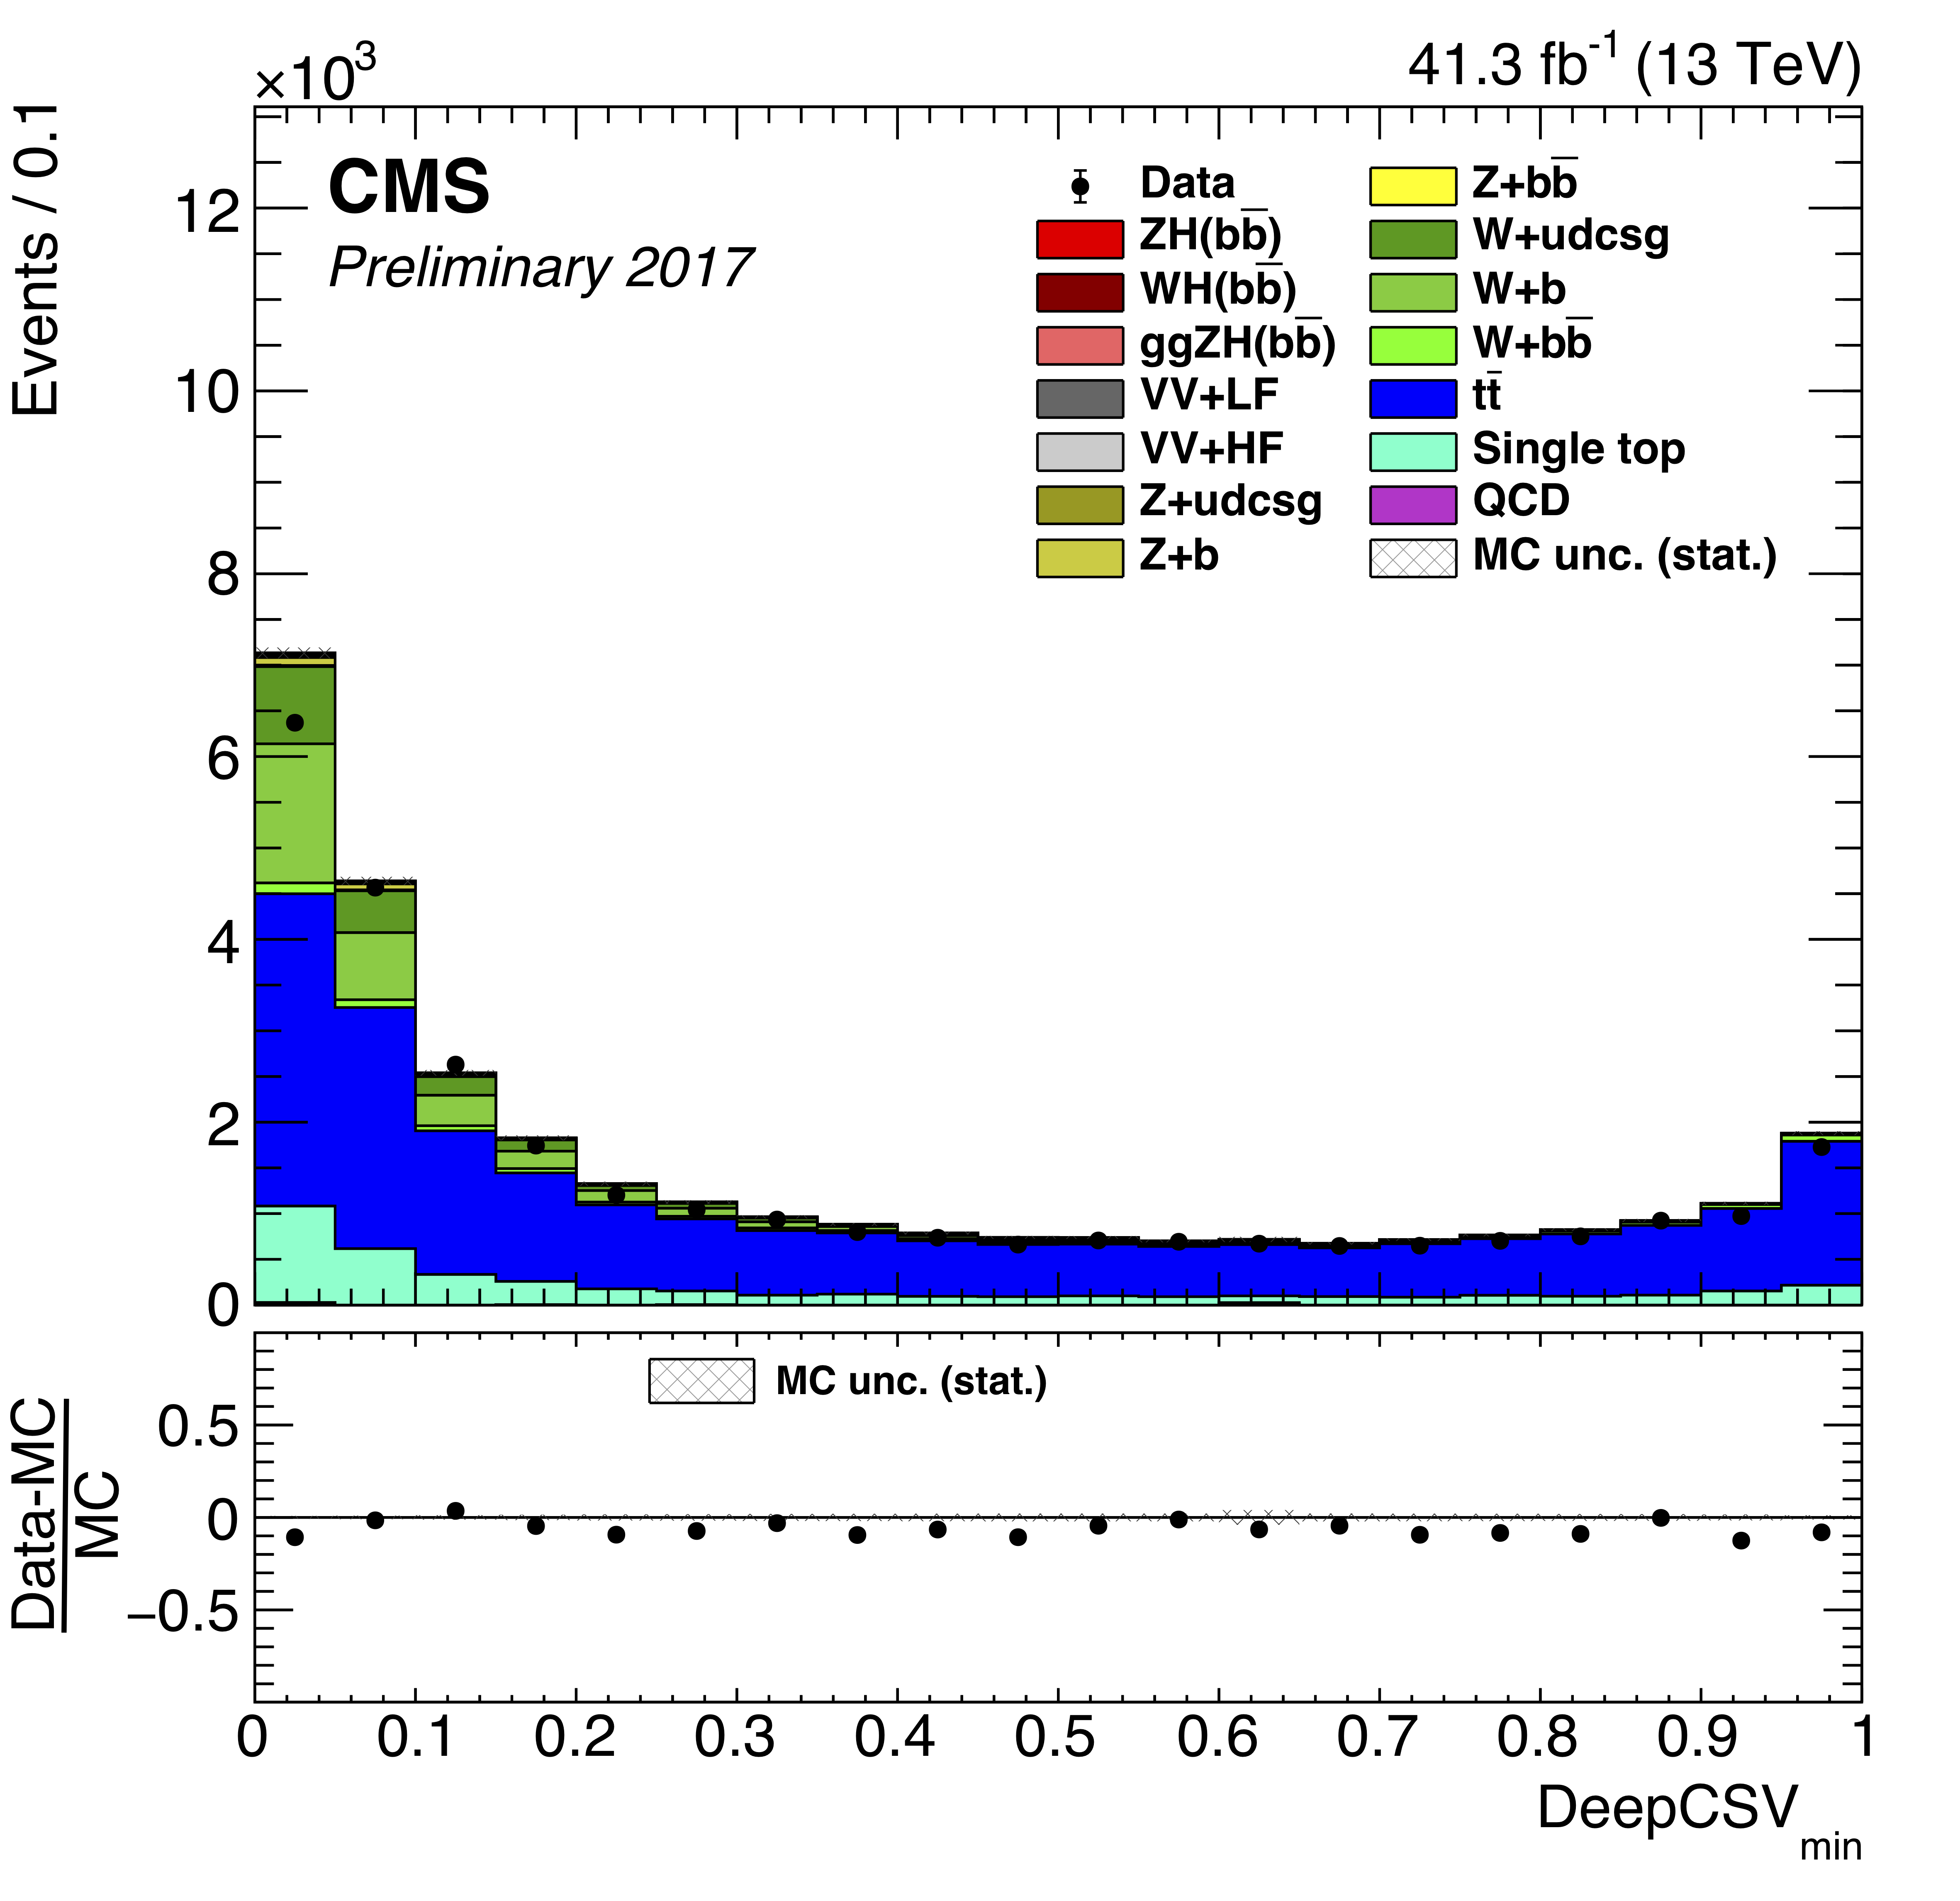
\includegraphics[width=0.39\linewidth]{images/CR_Wen_WHF_HighMjj/hJets_DeepCSV_1}}
    \subfigure [] {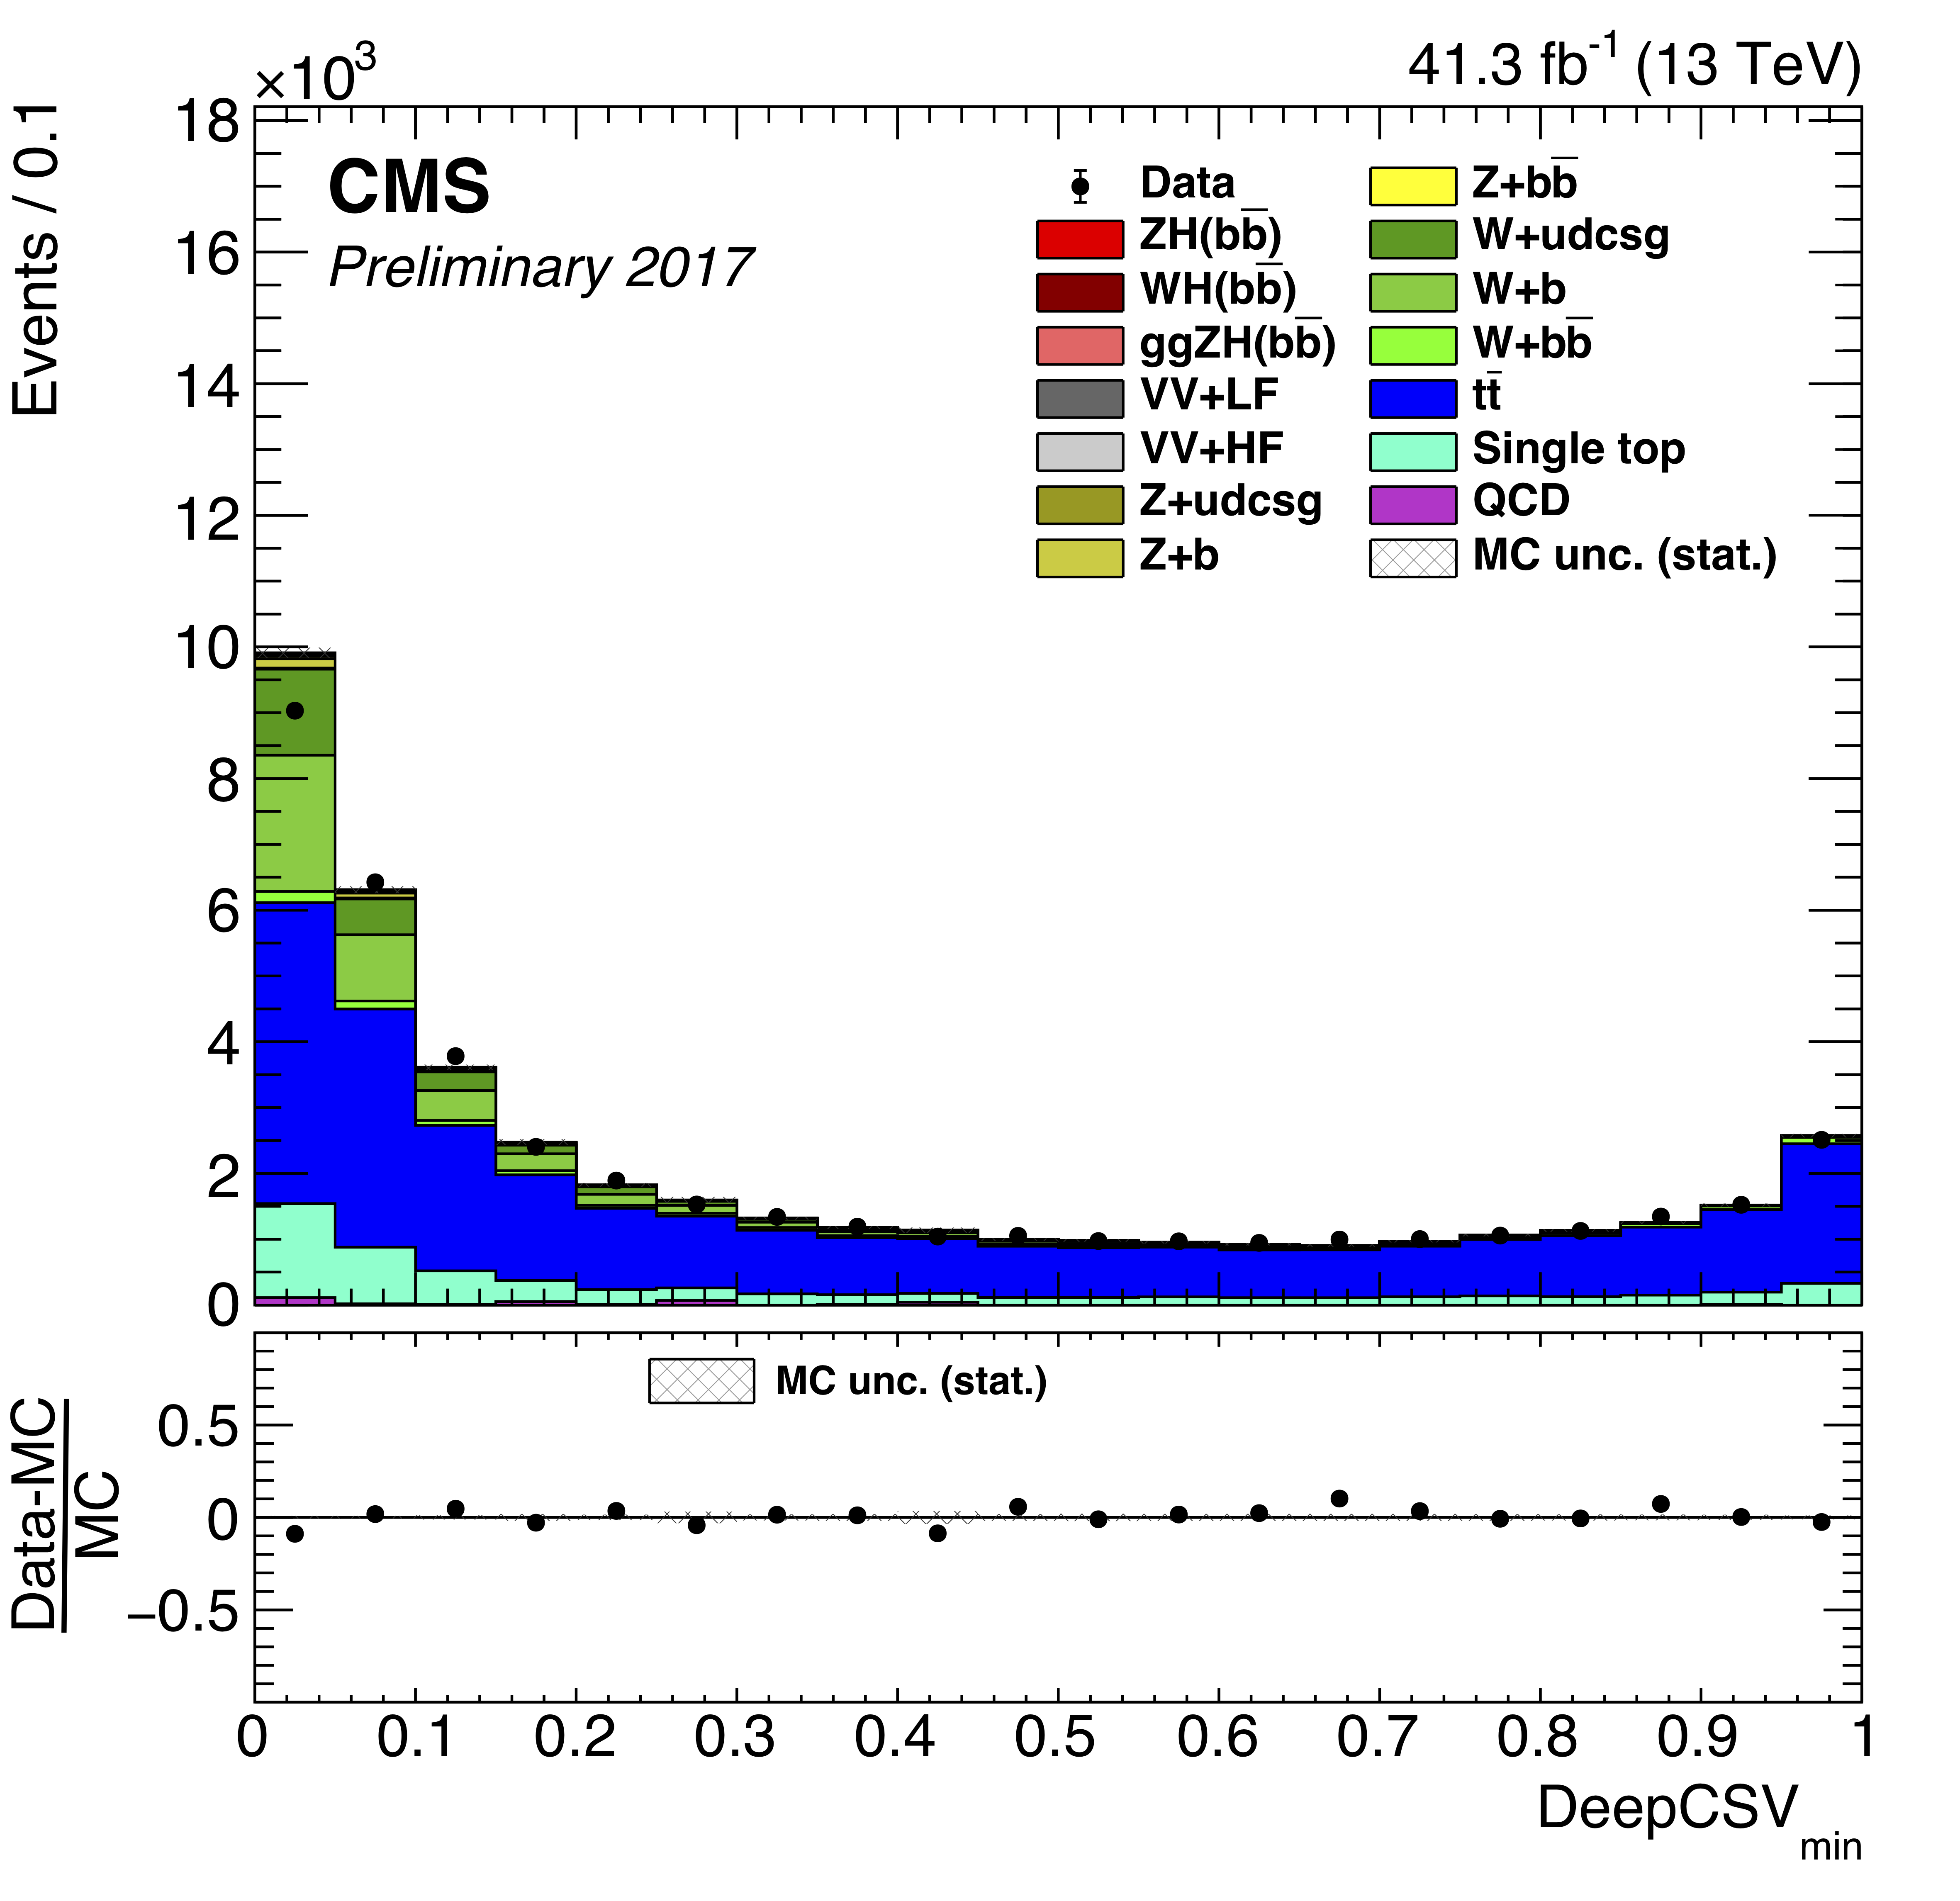
\includegraphics[width=0.39\linewidth]{images/CR_Wmn_WHF_HighMjj/hJets_DeepCSV_1}}
  }
  \caption[Control Region Distributions for the \WlnH\ Channels]{The distributions of variables of the \WenH\ channel (left column) and the \WmnH\ channel (right column): A), B) $\pT(jj) / \pT(\bosV)$ for the \qrkt\qrktbar\ control region; C), D) $m(jj)$ for the \bosW+light control region; E), F) \btagmin\ for the high mass \bosW+heavy control region.}
  \label{fig:CR_Wln}
\end{figure}

\clearpage

%%%%%%%%%%%%%%%%%%%
% ZllHbb, Low VPt %
%%%%%%%%%%%%%%%%%%%

\begin{figure}[htbp]
  \centering
  \mbox{
    \subfigure [] {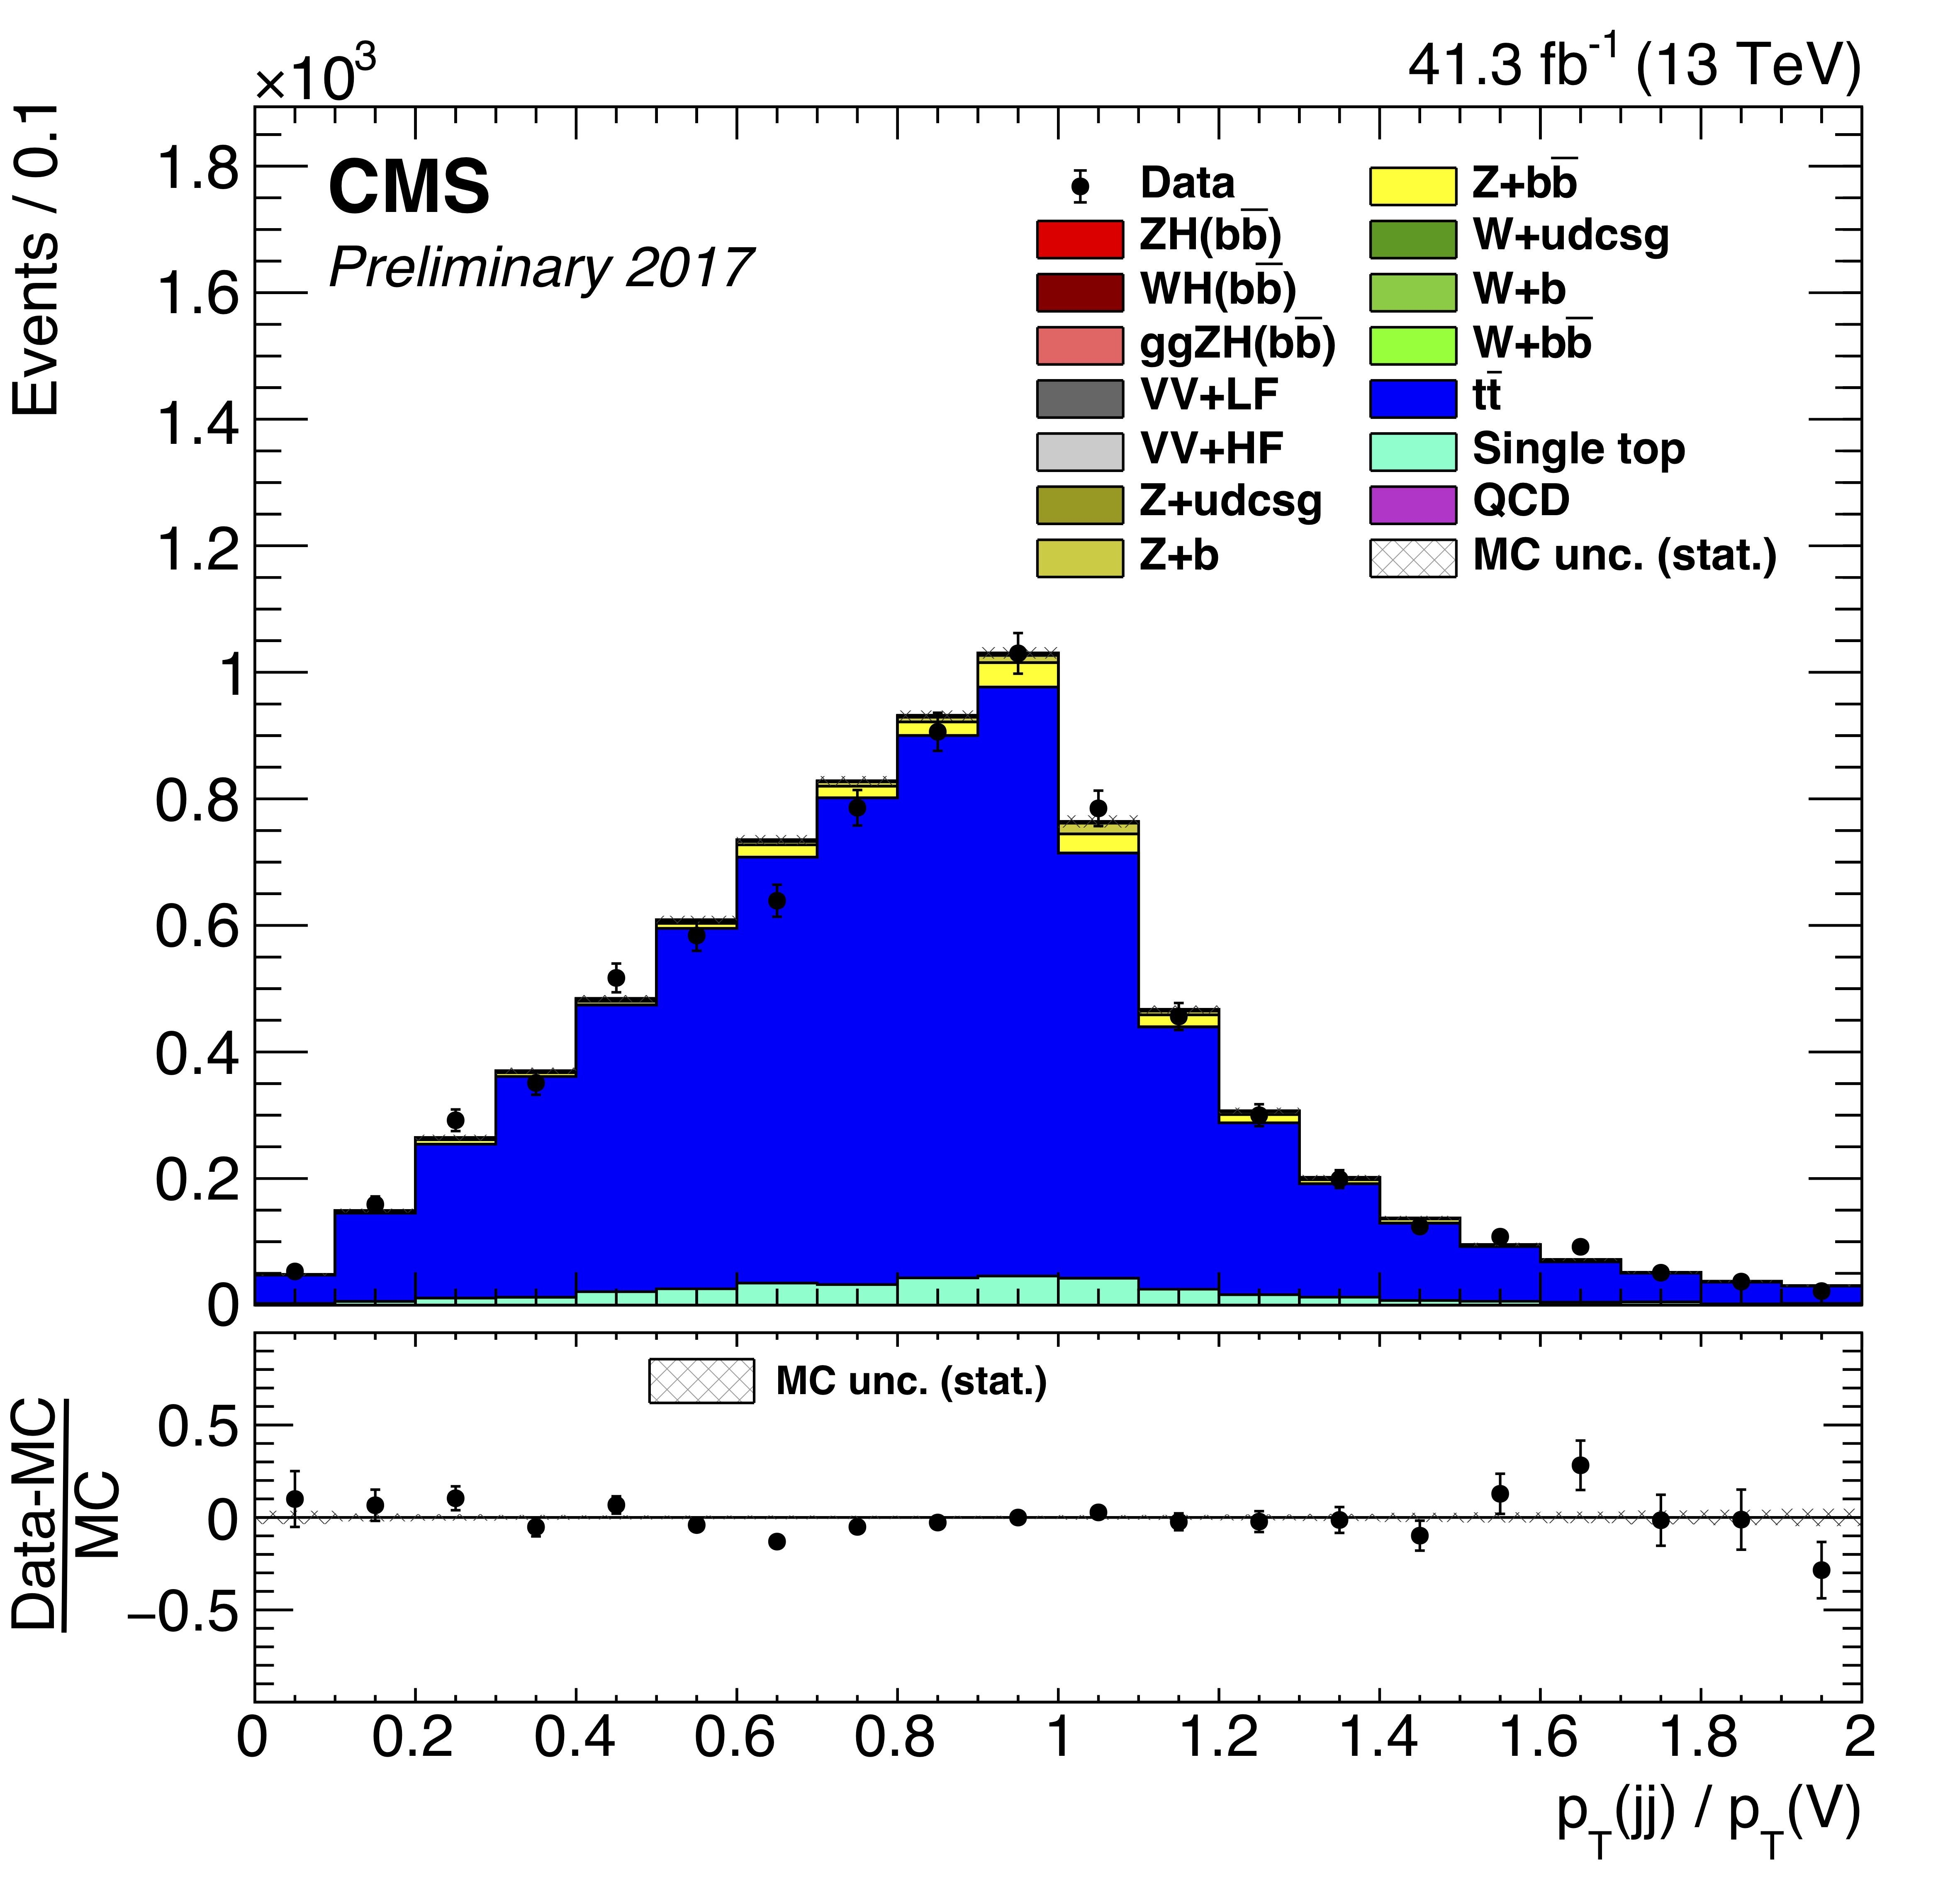
\includegraphics[width=0.39\linewidth]{images/CR_ZeeLowPt_TT/jjVPtRatio_fit}}
    \subfigure [] {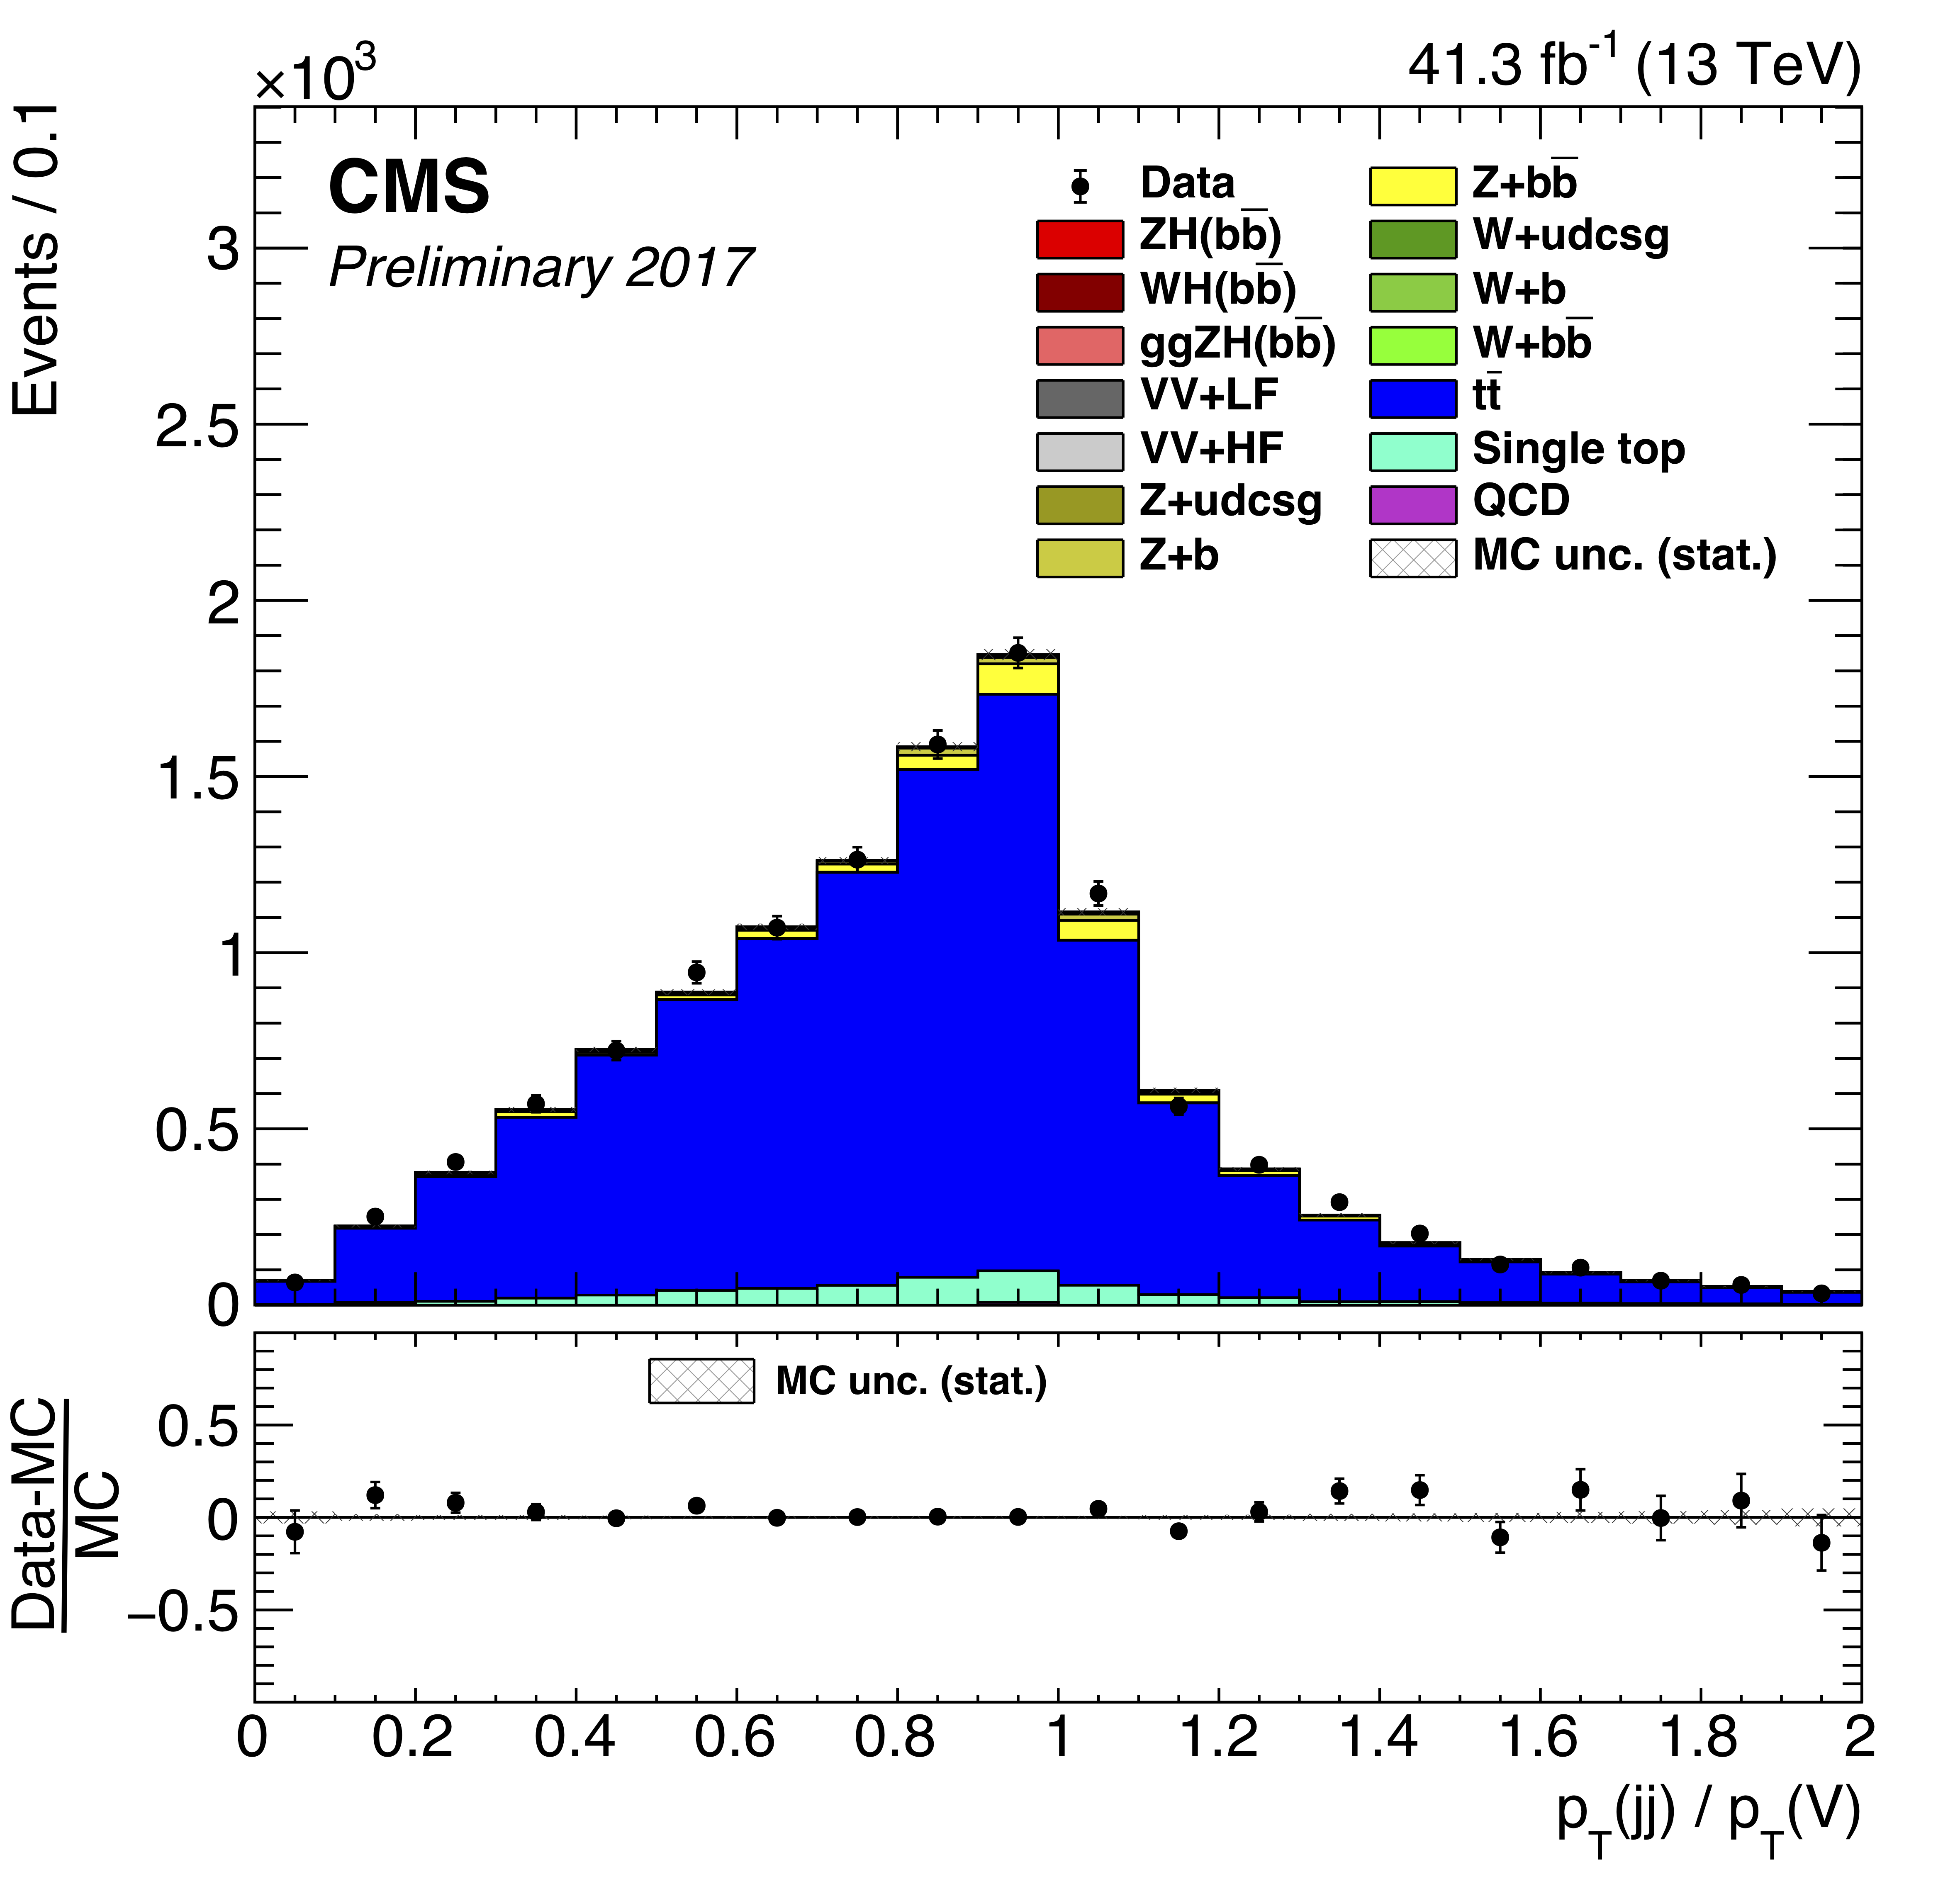
\includegraphics[width=0.39\linewidth]{images/CR_ZmmLowPt_TT/jjVPtRatio_fit}}
  }
  \mbox{
    \subfigure [] {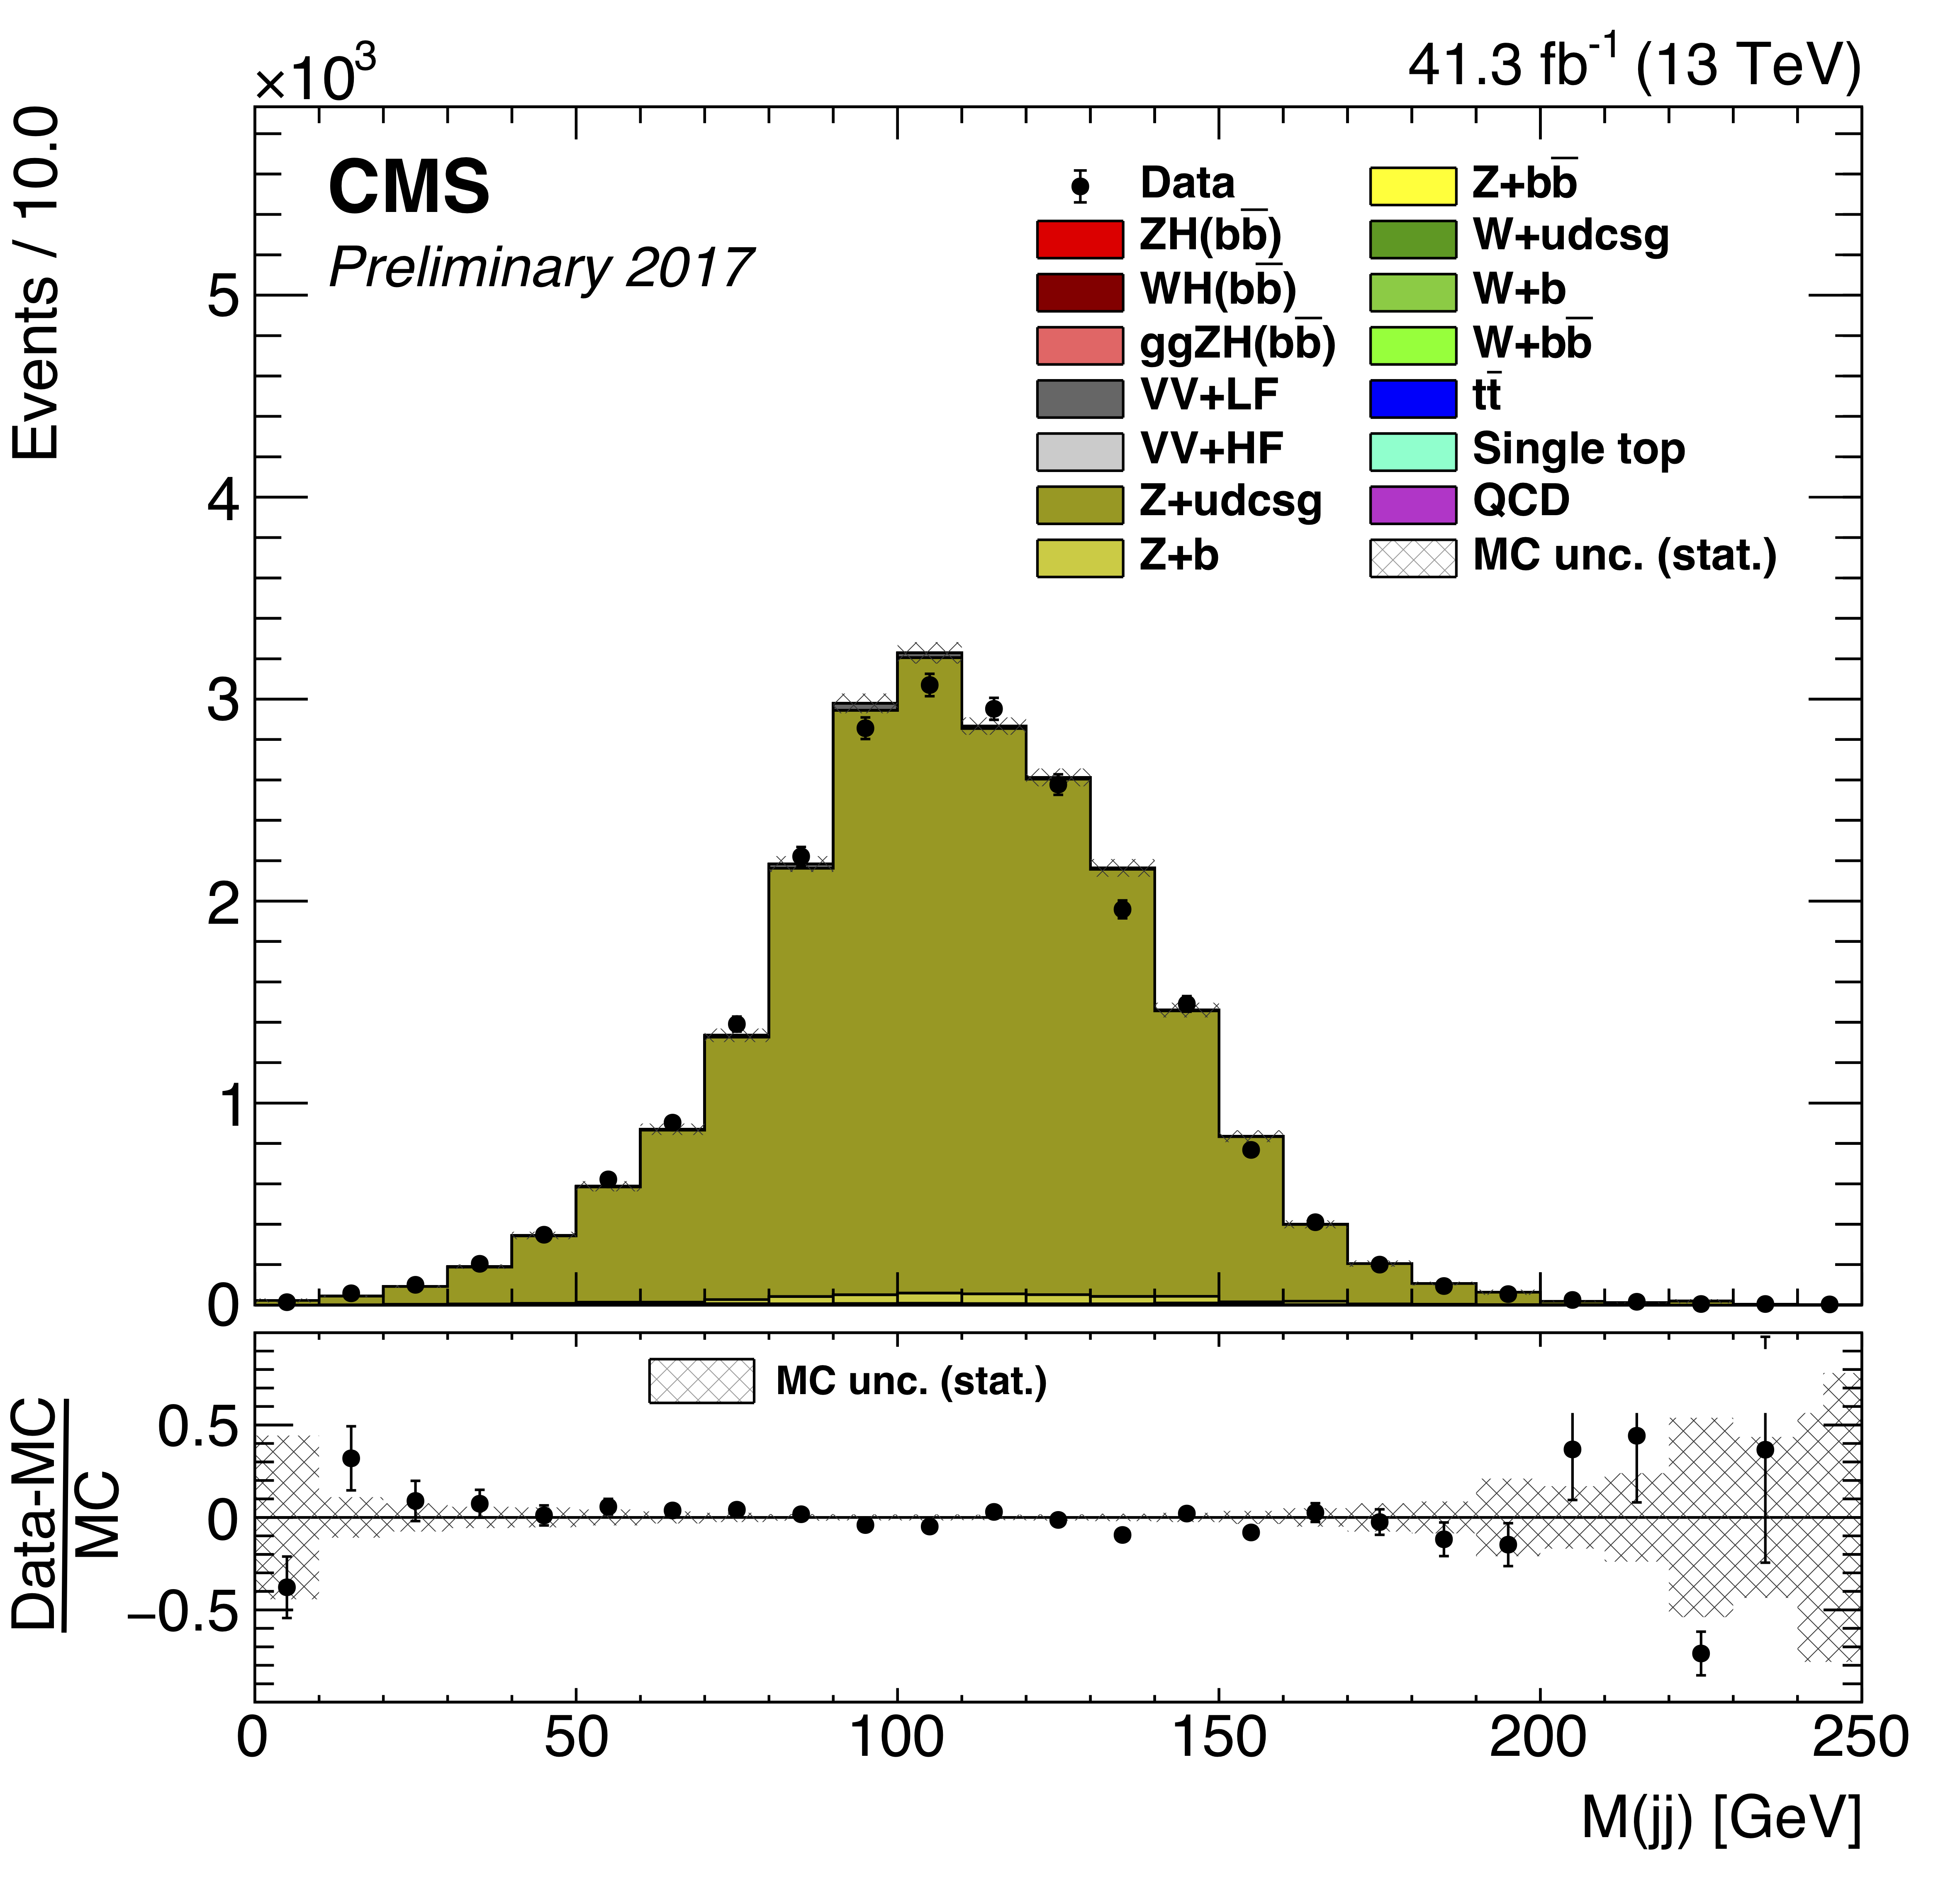
\includegraphics[width=0.39\linewidth]{images/CR_ZeeLowPt_ZLF/H_mass_fit}}
    \subfigure [] {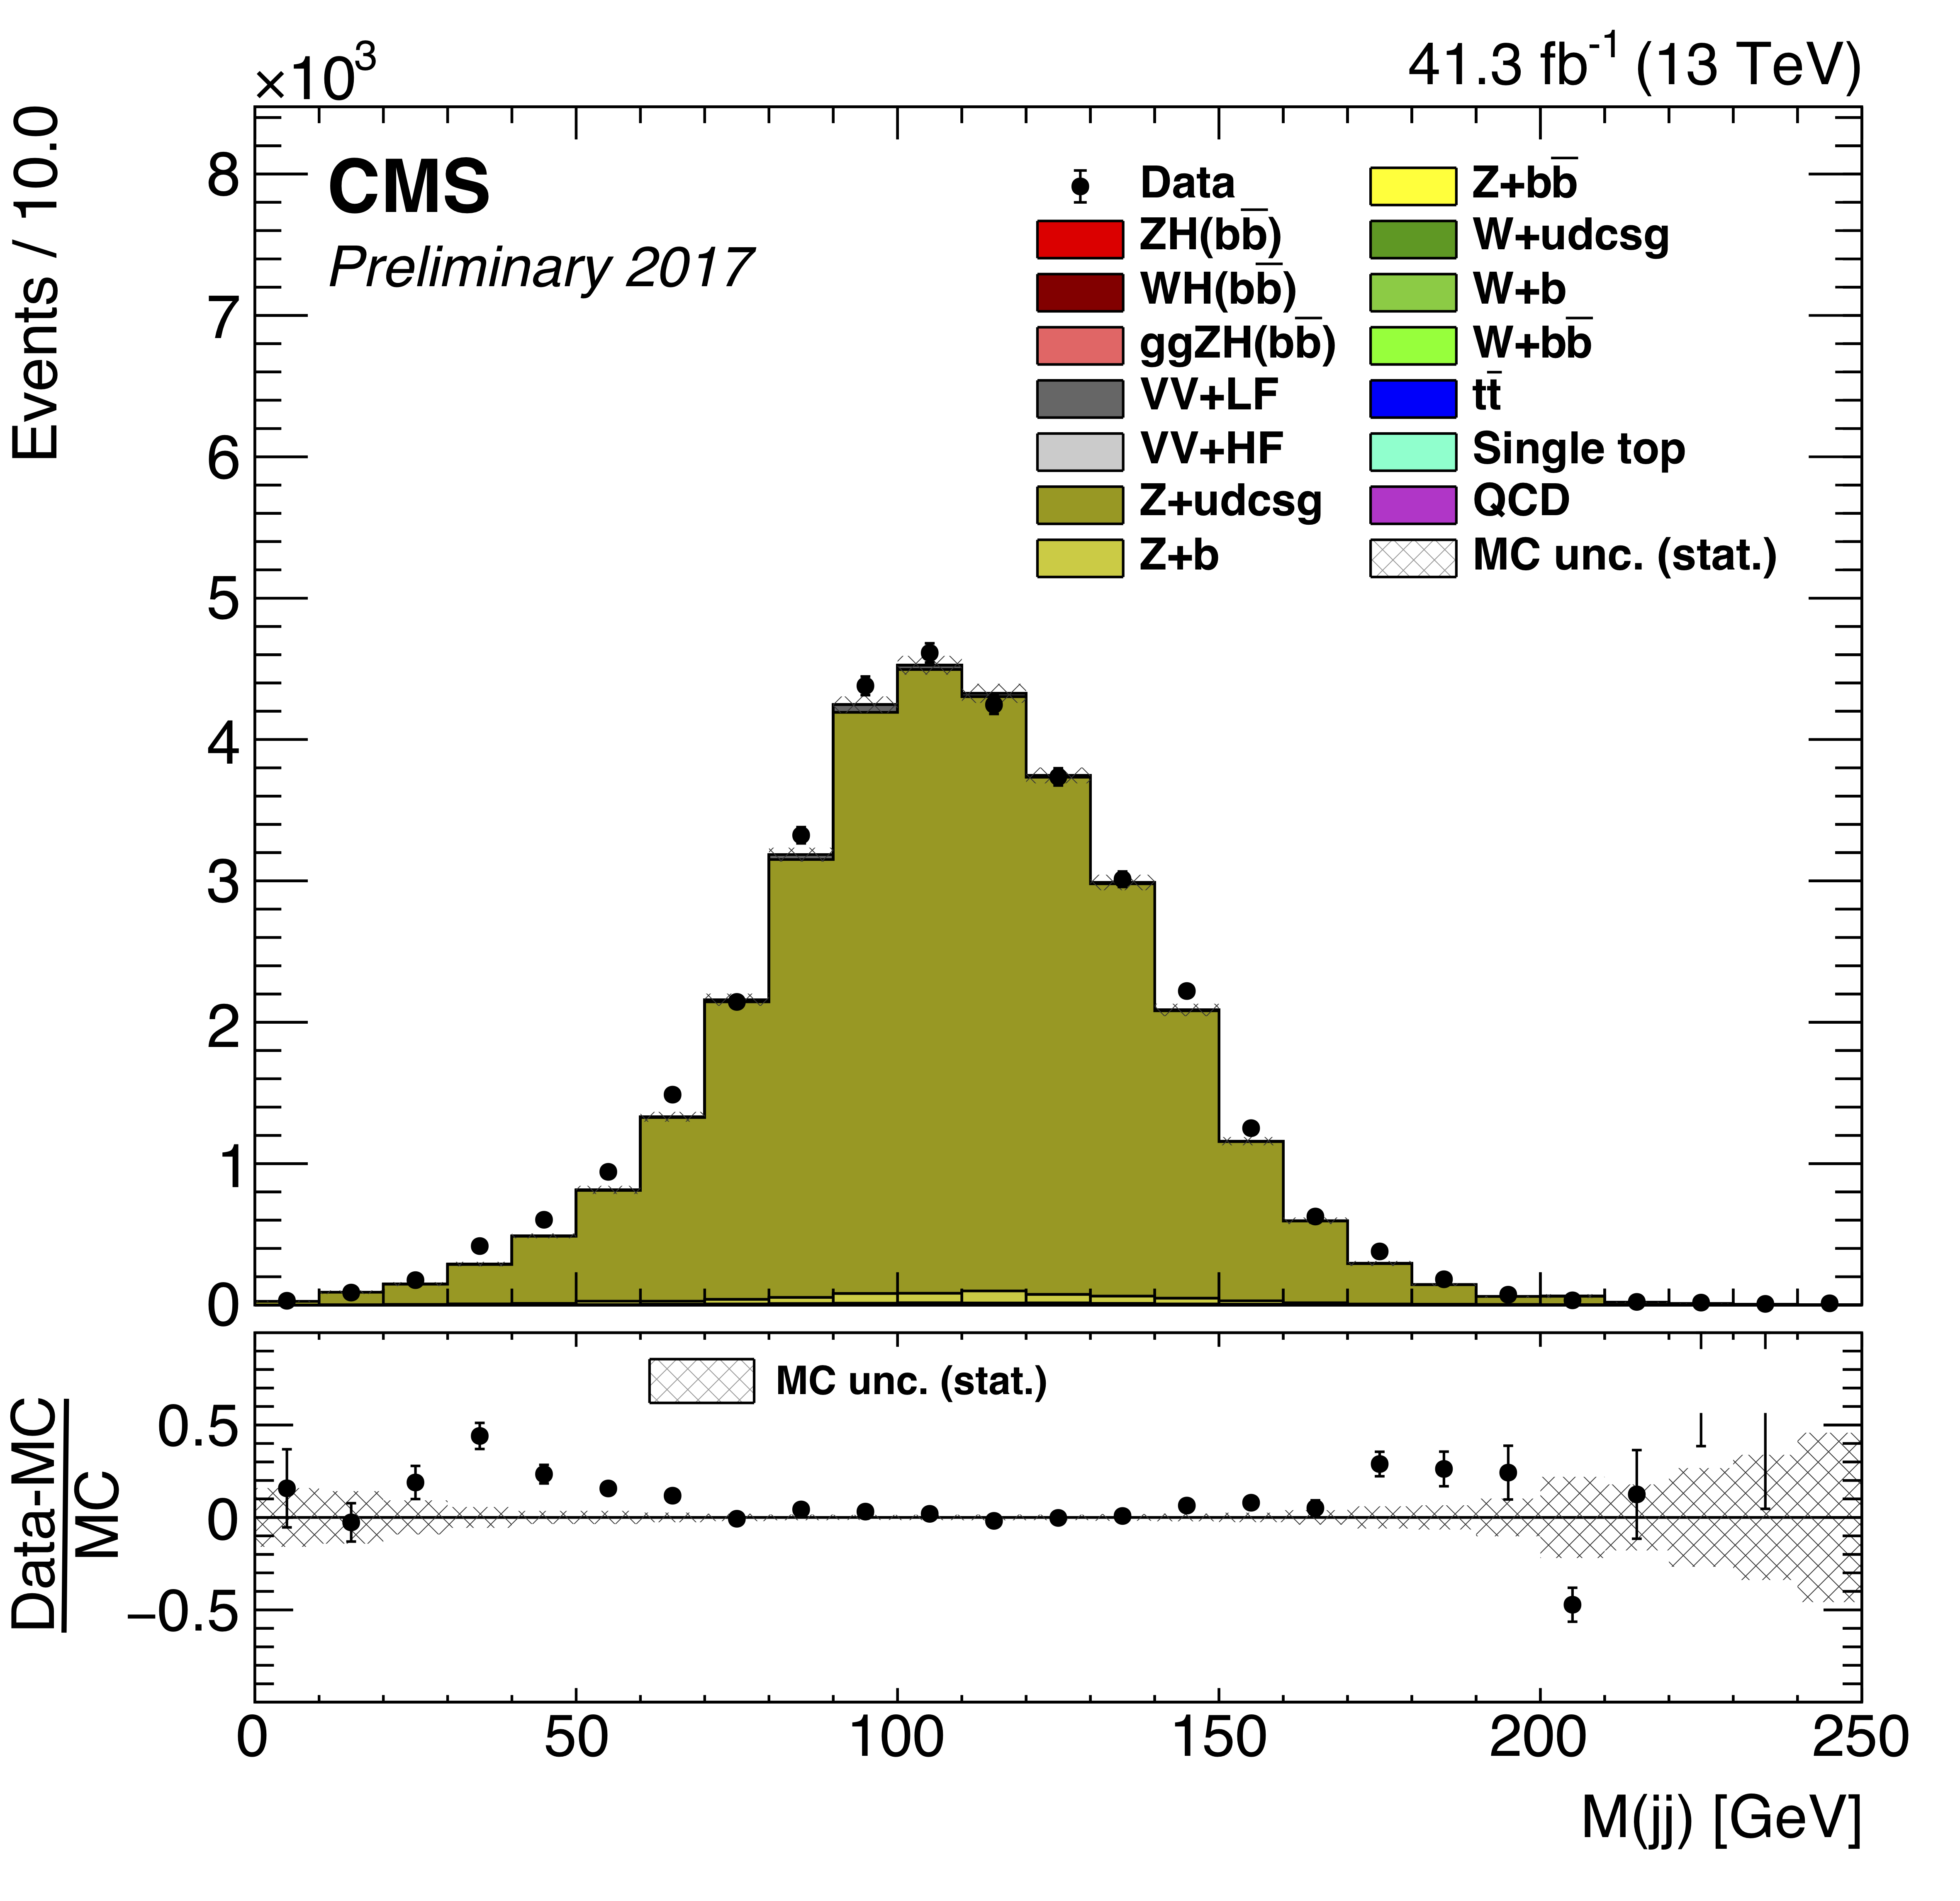
\includegraphics[width=0.39\linewidth]{images/CR_ZmmLowPt_ZLF/H_mass_fit}}
  }
  \mbox{
    \subfigure [] {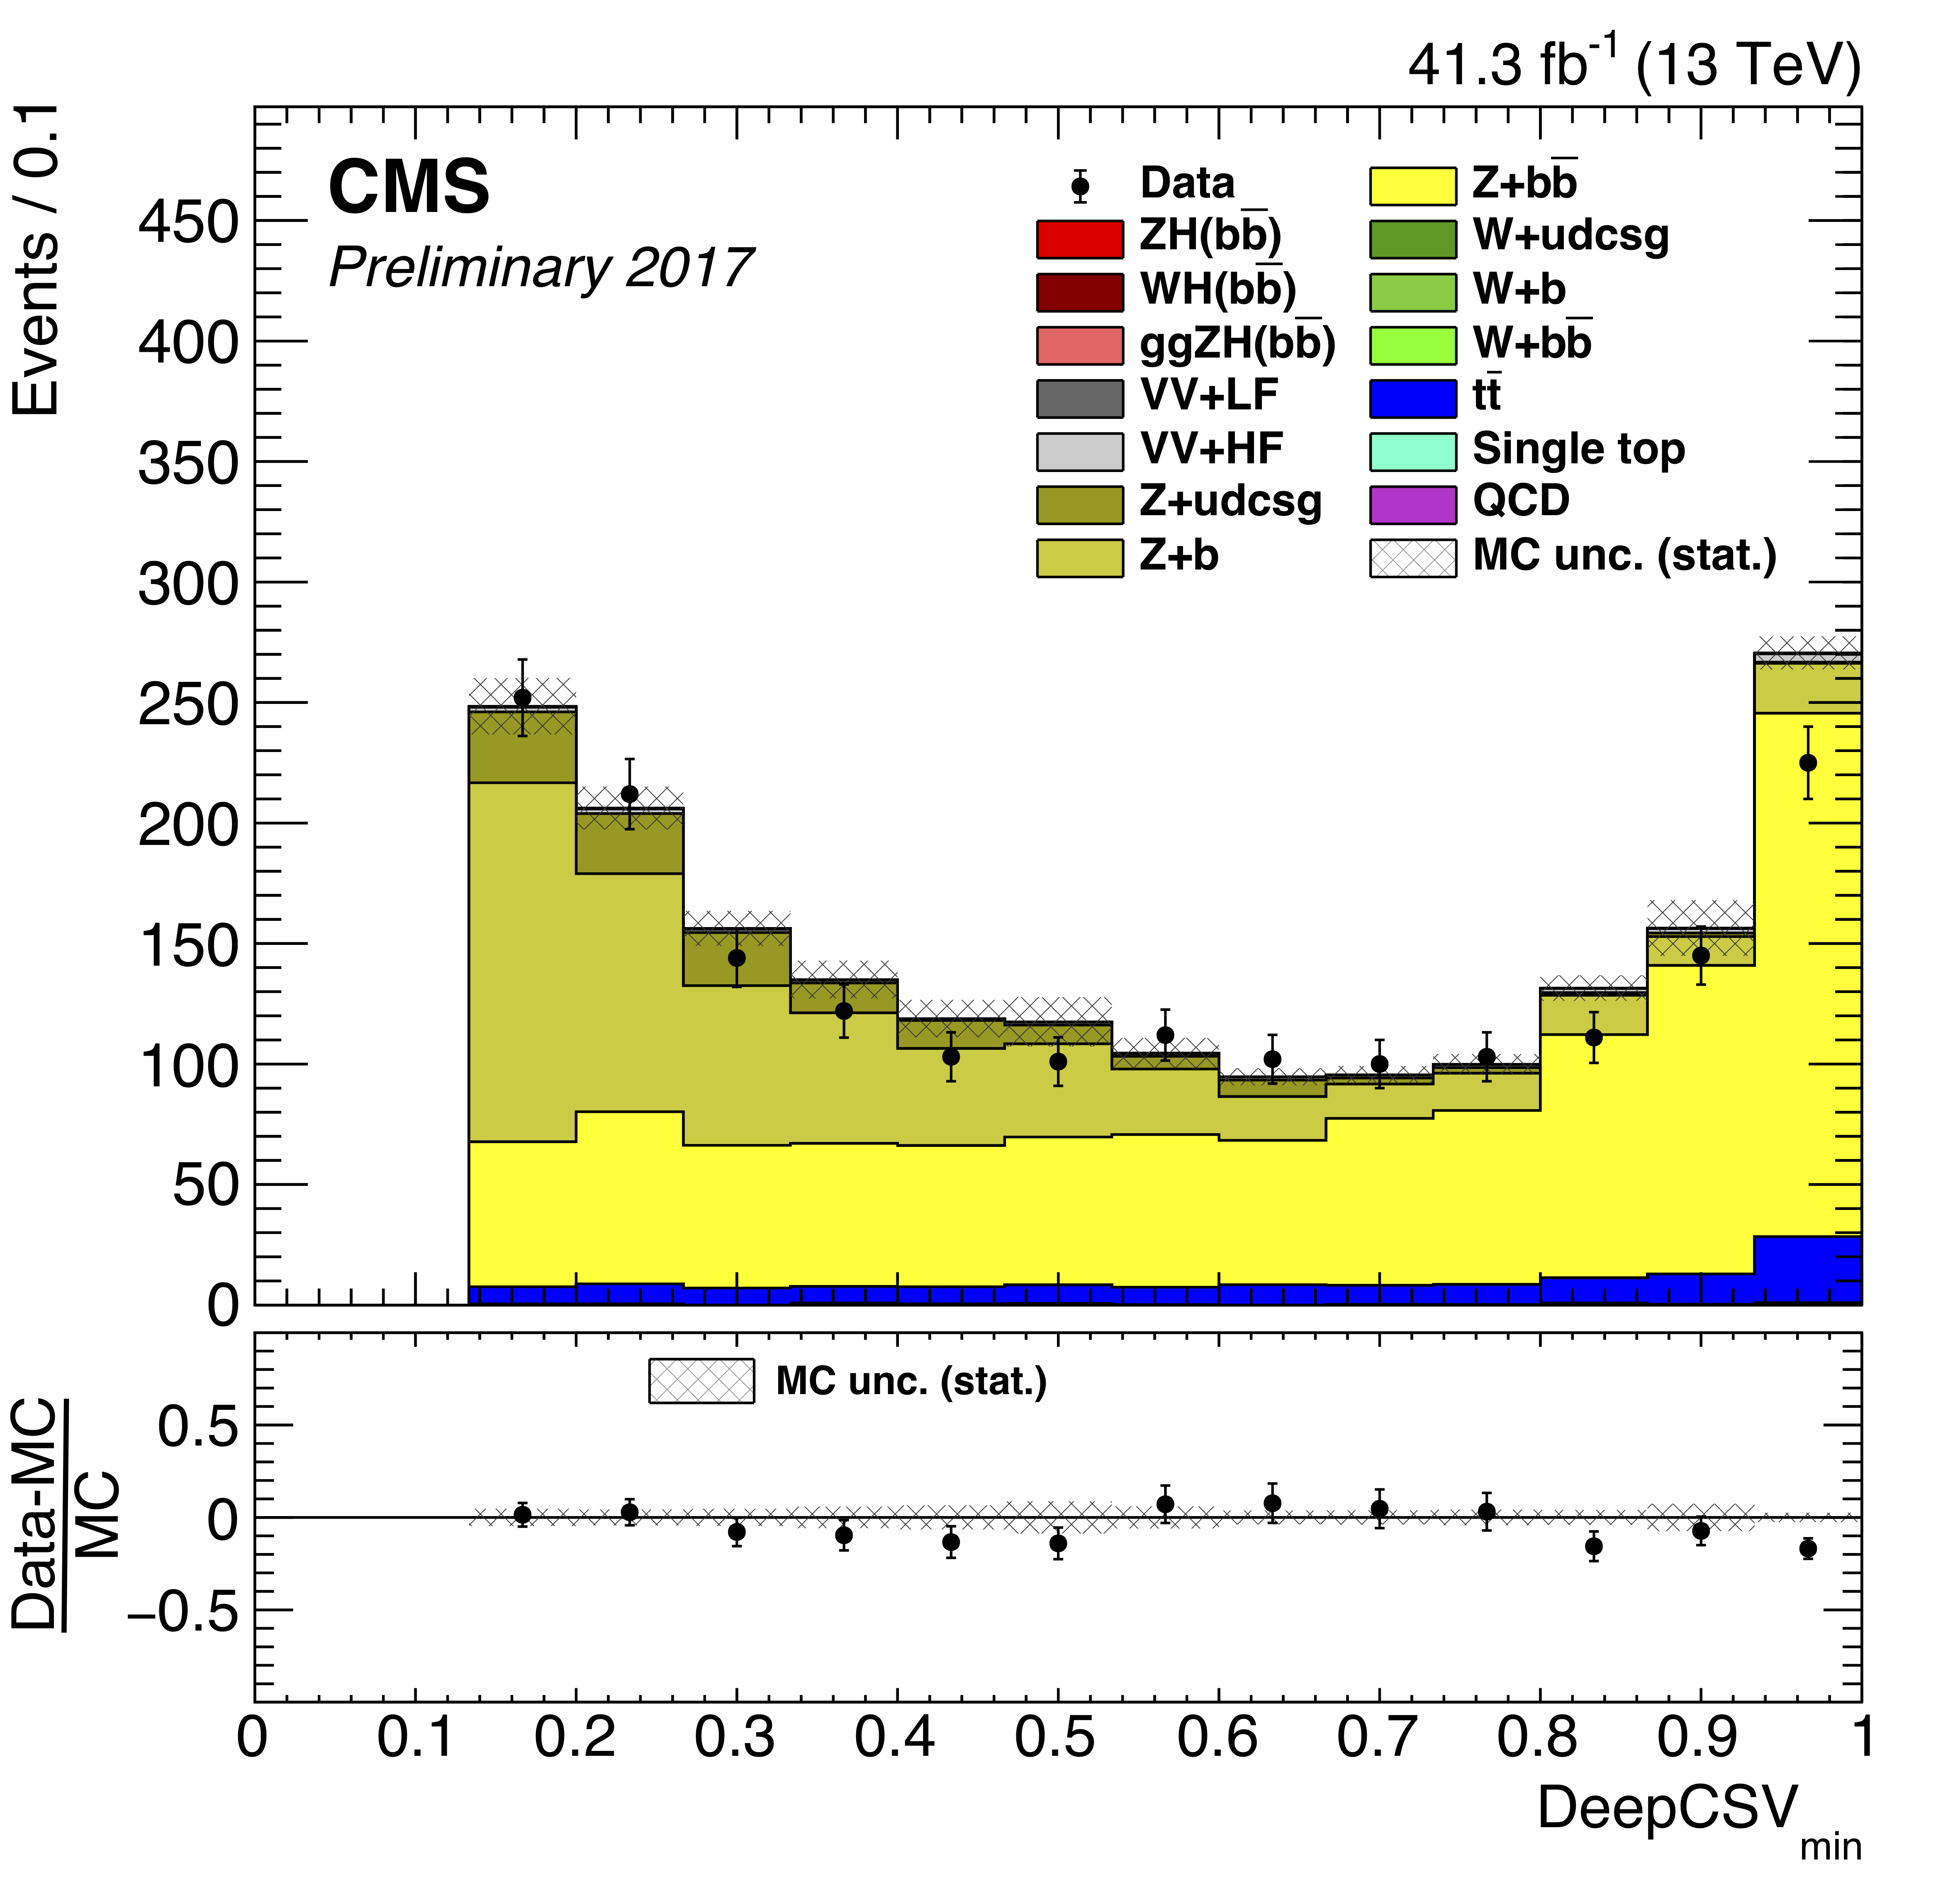
\includegraphics[width=0.39\linewidth]{images/CR_ZeeLowPt_ZHF/hJets_DeepCSV_1}}
    \subfigure [] {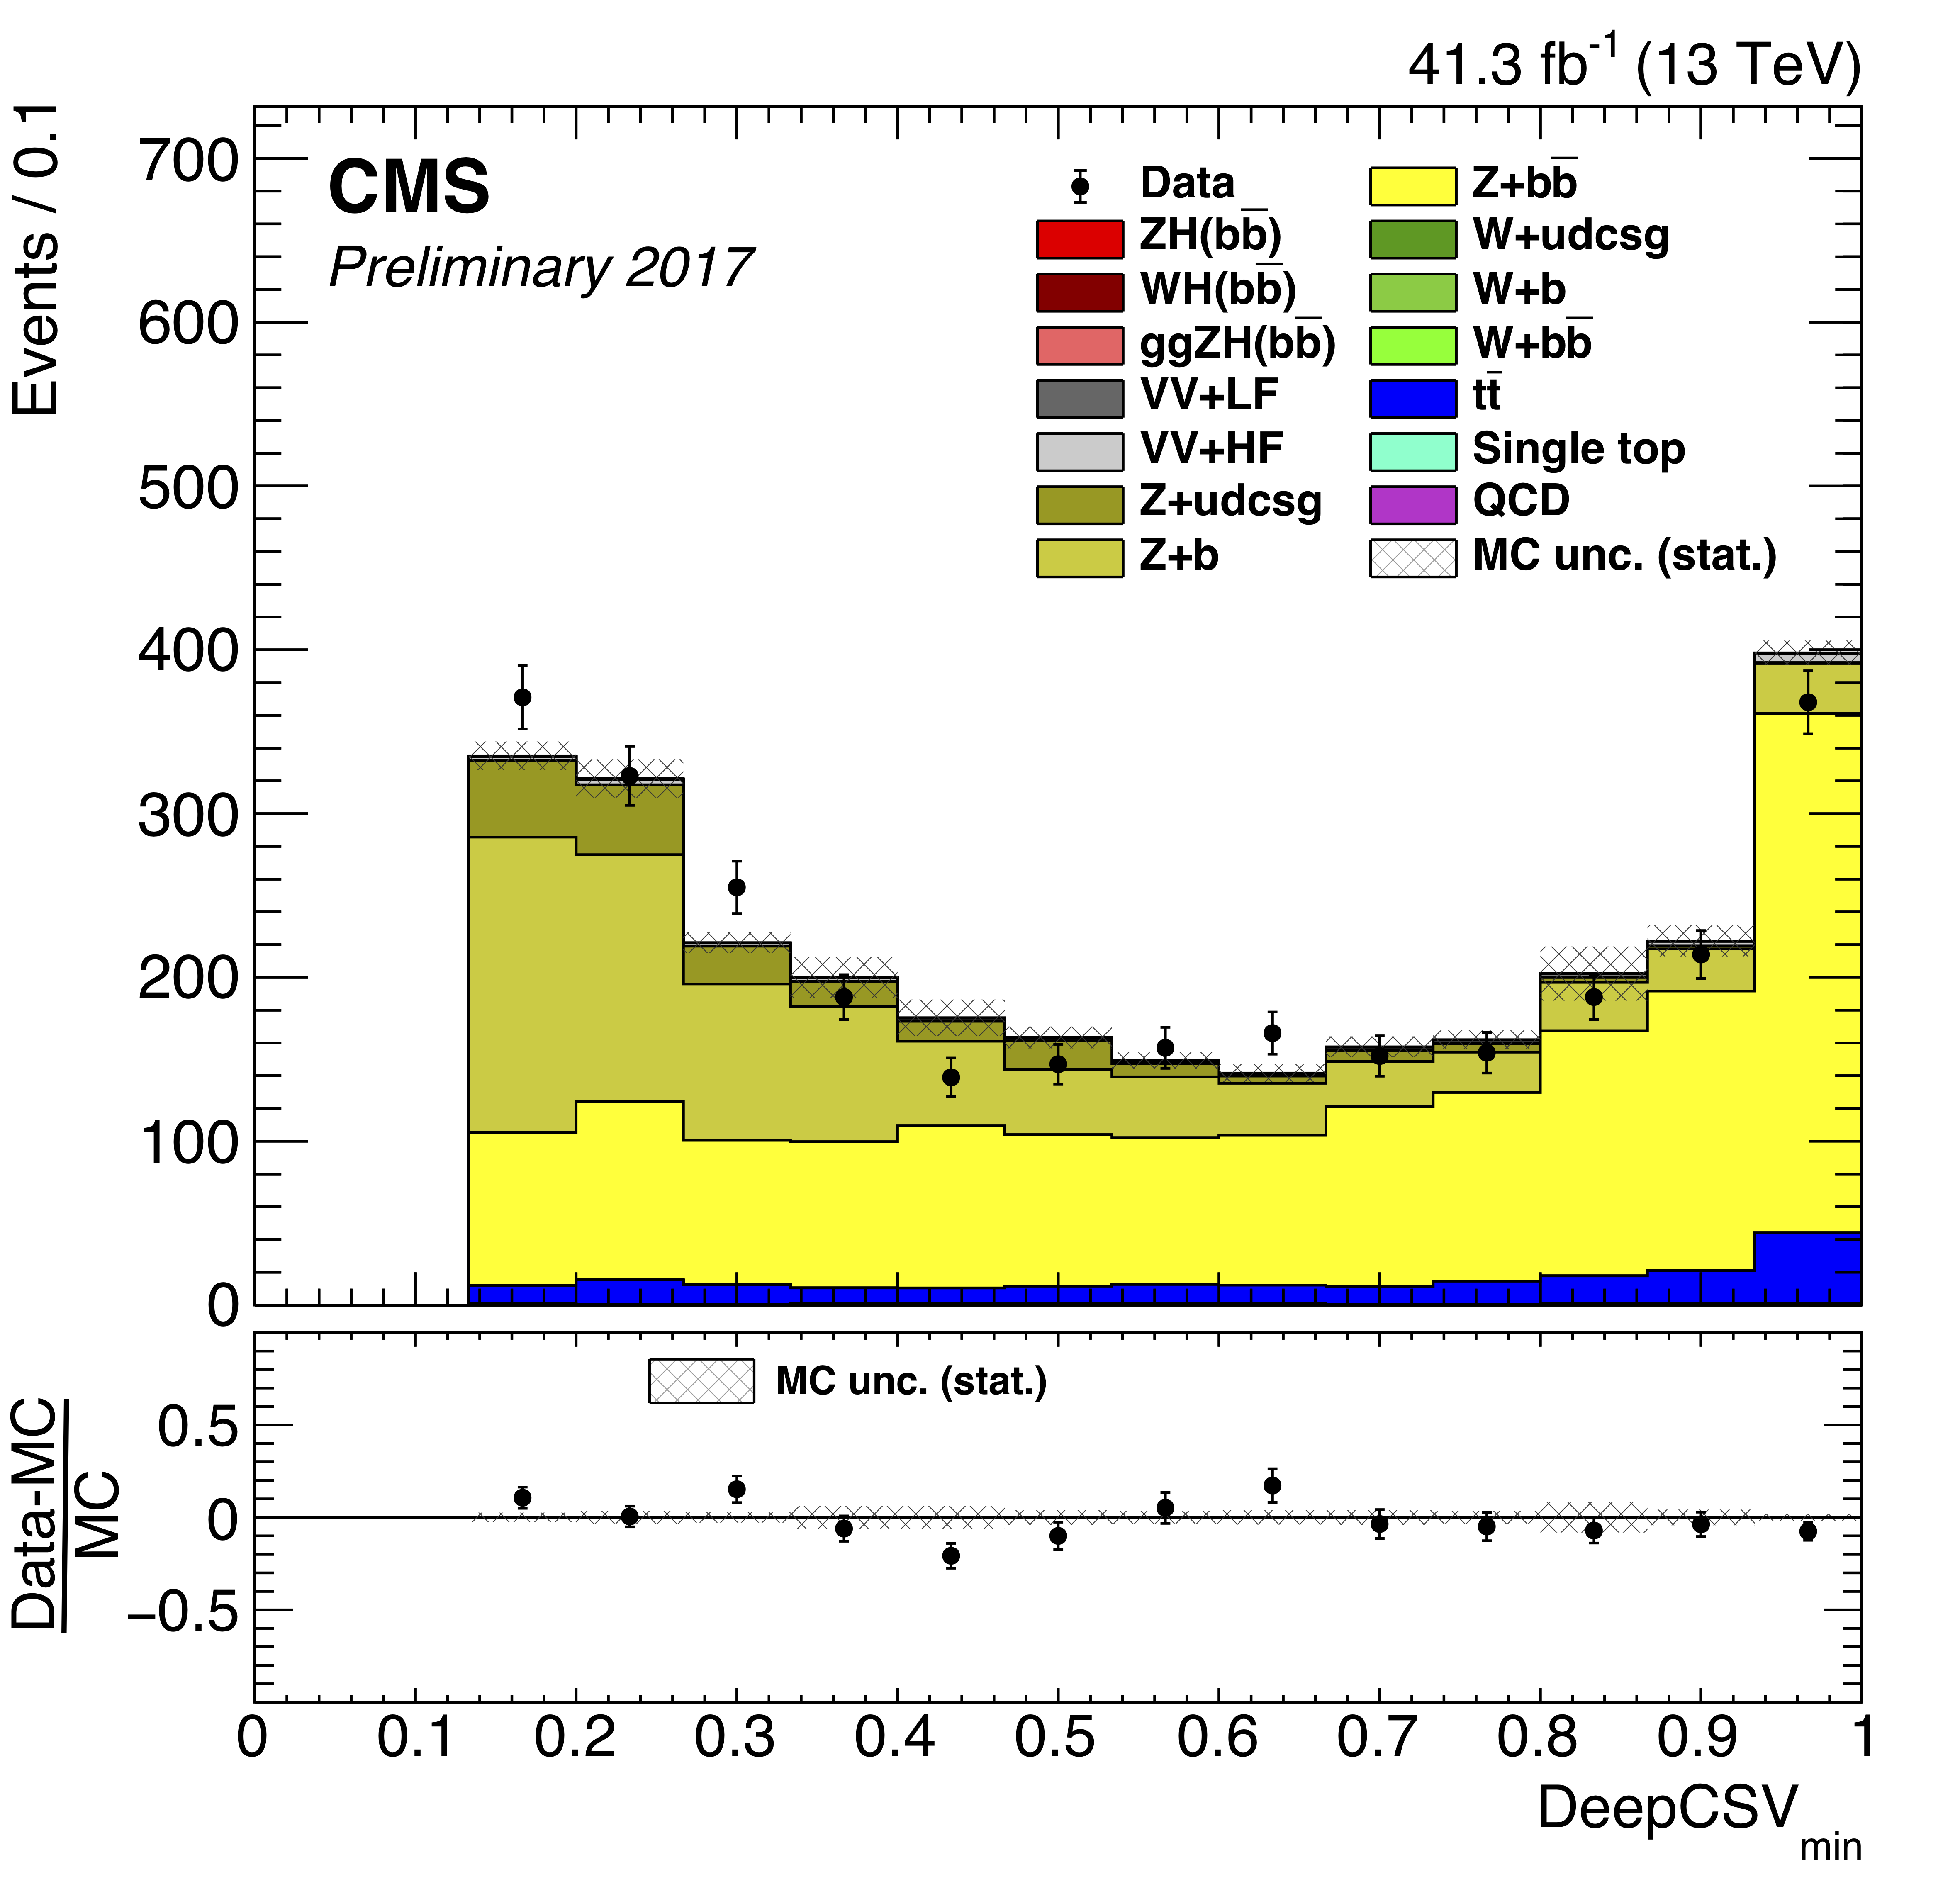
\includegraphics[width=0.39\linewidth]{images/CR_ZmmLowPt_ZHF/hJets_DeepCSV_1}}
  }
  \caption[Low $\pT(\bosV)$ Control Region Distributions for the \ZllH\ Channels]{The distributions of variables of the \ZeeH\ channel (left column) and the \ZmmH\ channel (right column) in the low $\pT(\bosV)$ region: A), B) $\pT(jj) / \pT(\bosV)$ for the \qrkt\qrktbar\ control region; C), D) $m(jj)$ for the \bosZ+light control region; E), F) \btagmin\ for the \bosZ+heavy control region.}
  \label{fig:CR_Zll_LowPt}
\end{figure}

\clearpage

%%%%%%%%%%%%%%%%%%%%
% ZllHbb, High VPt %
%%%%%%%%%%%%%%%%%%%%

\begin{figure}[htbp]
  \centering
  \mbox{
    \subfigure [] {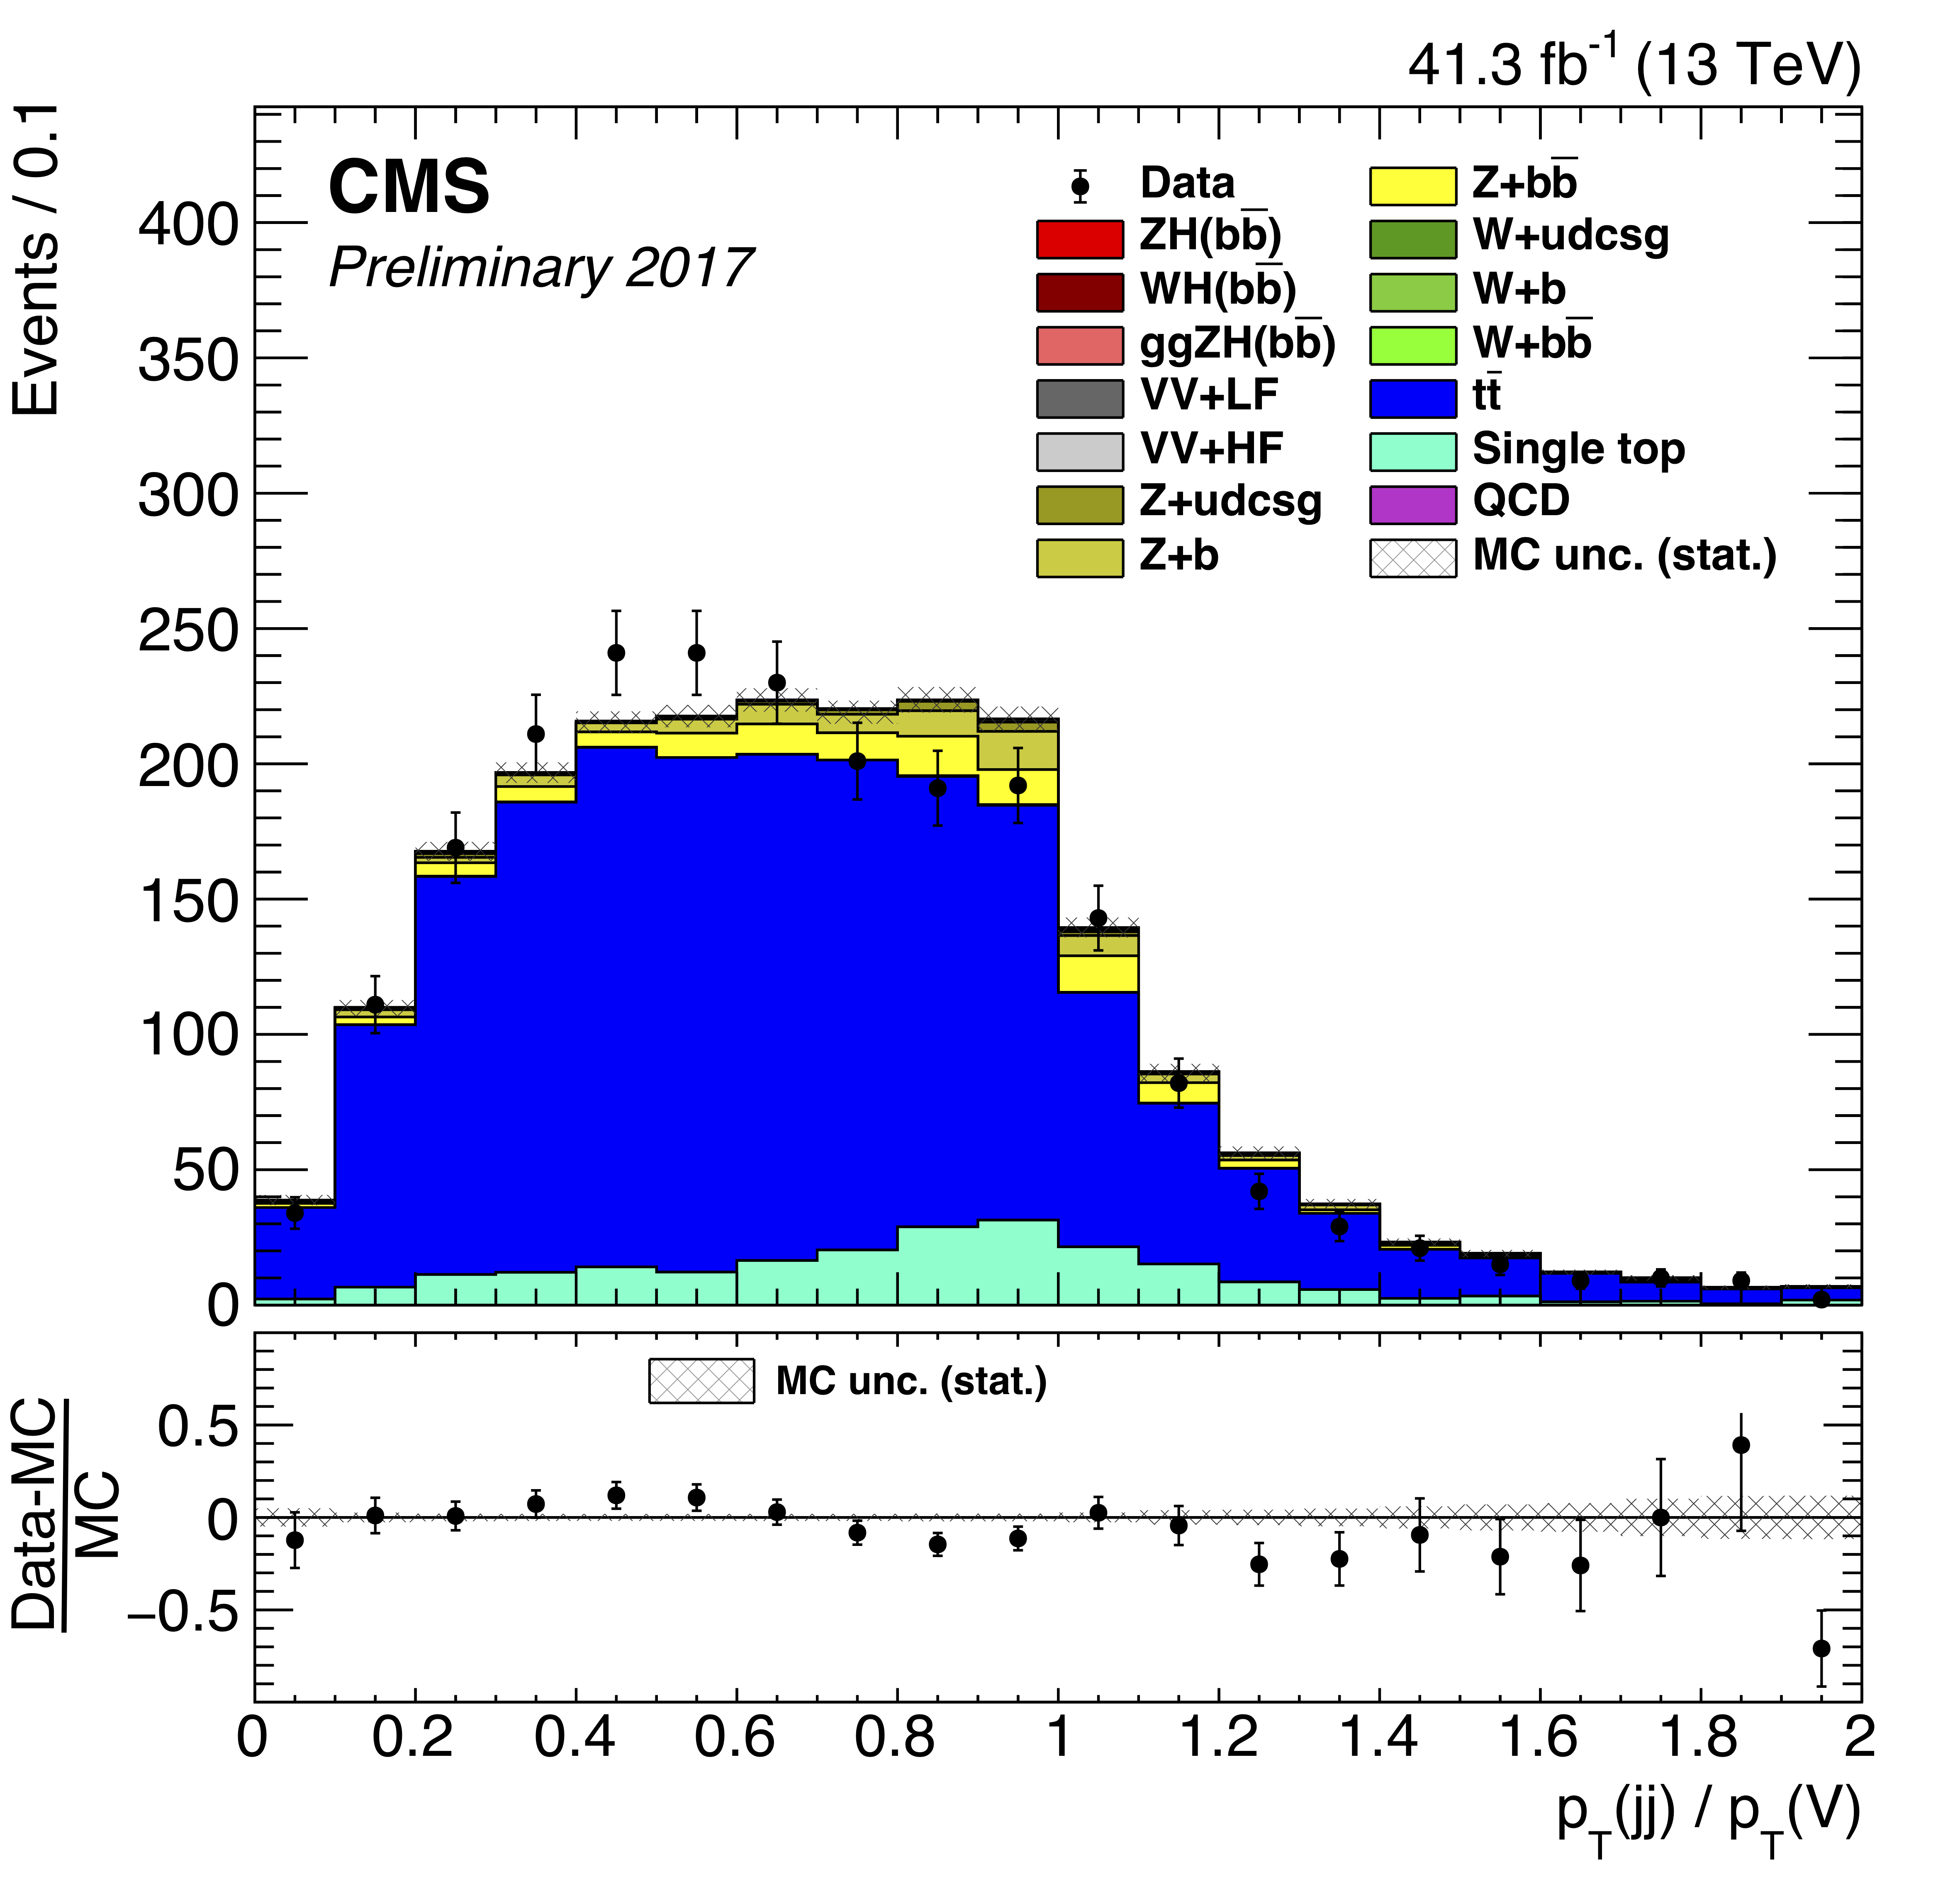
\includegraphics[width=0.39\linewidth]{images/CR_ZeeHighPt_TT/jjVPtRatio_fit}}
    \subfigure [] {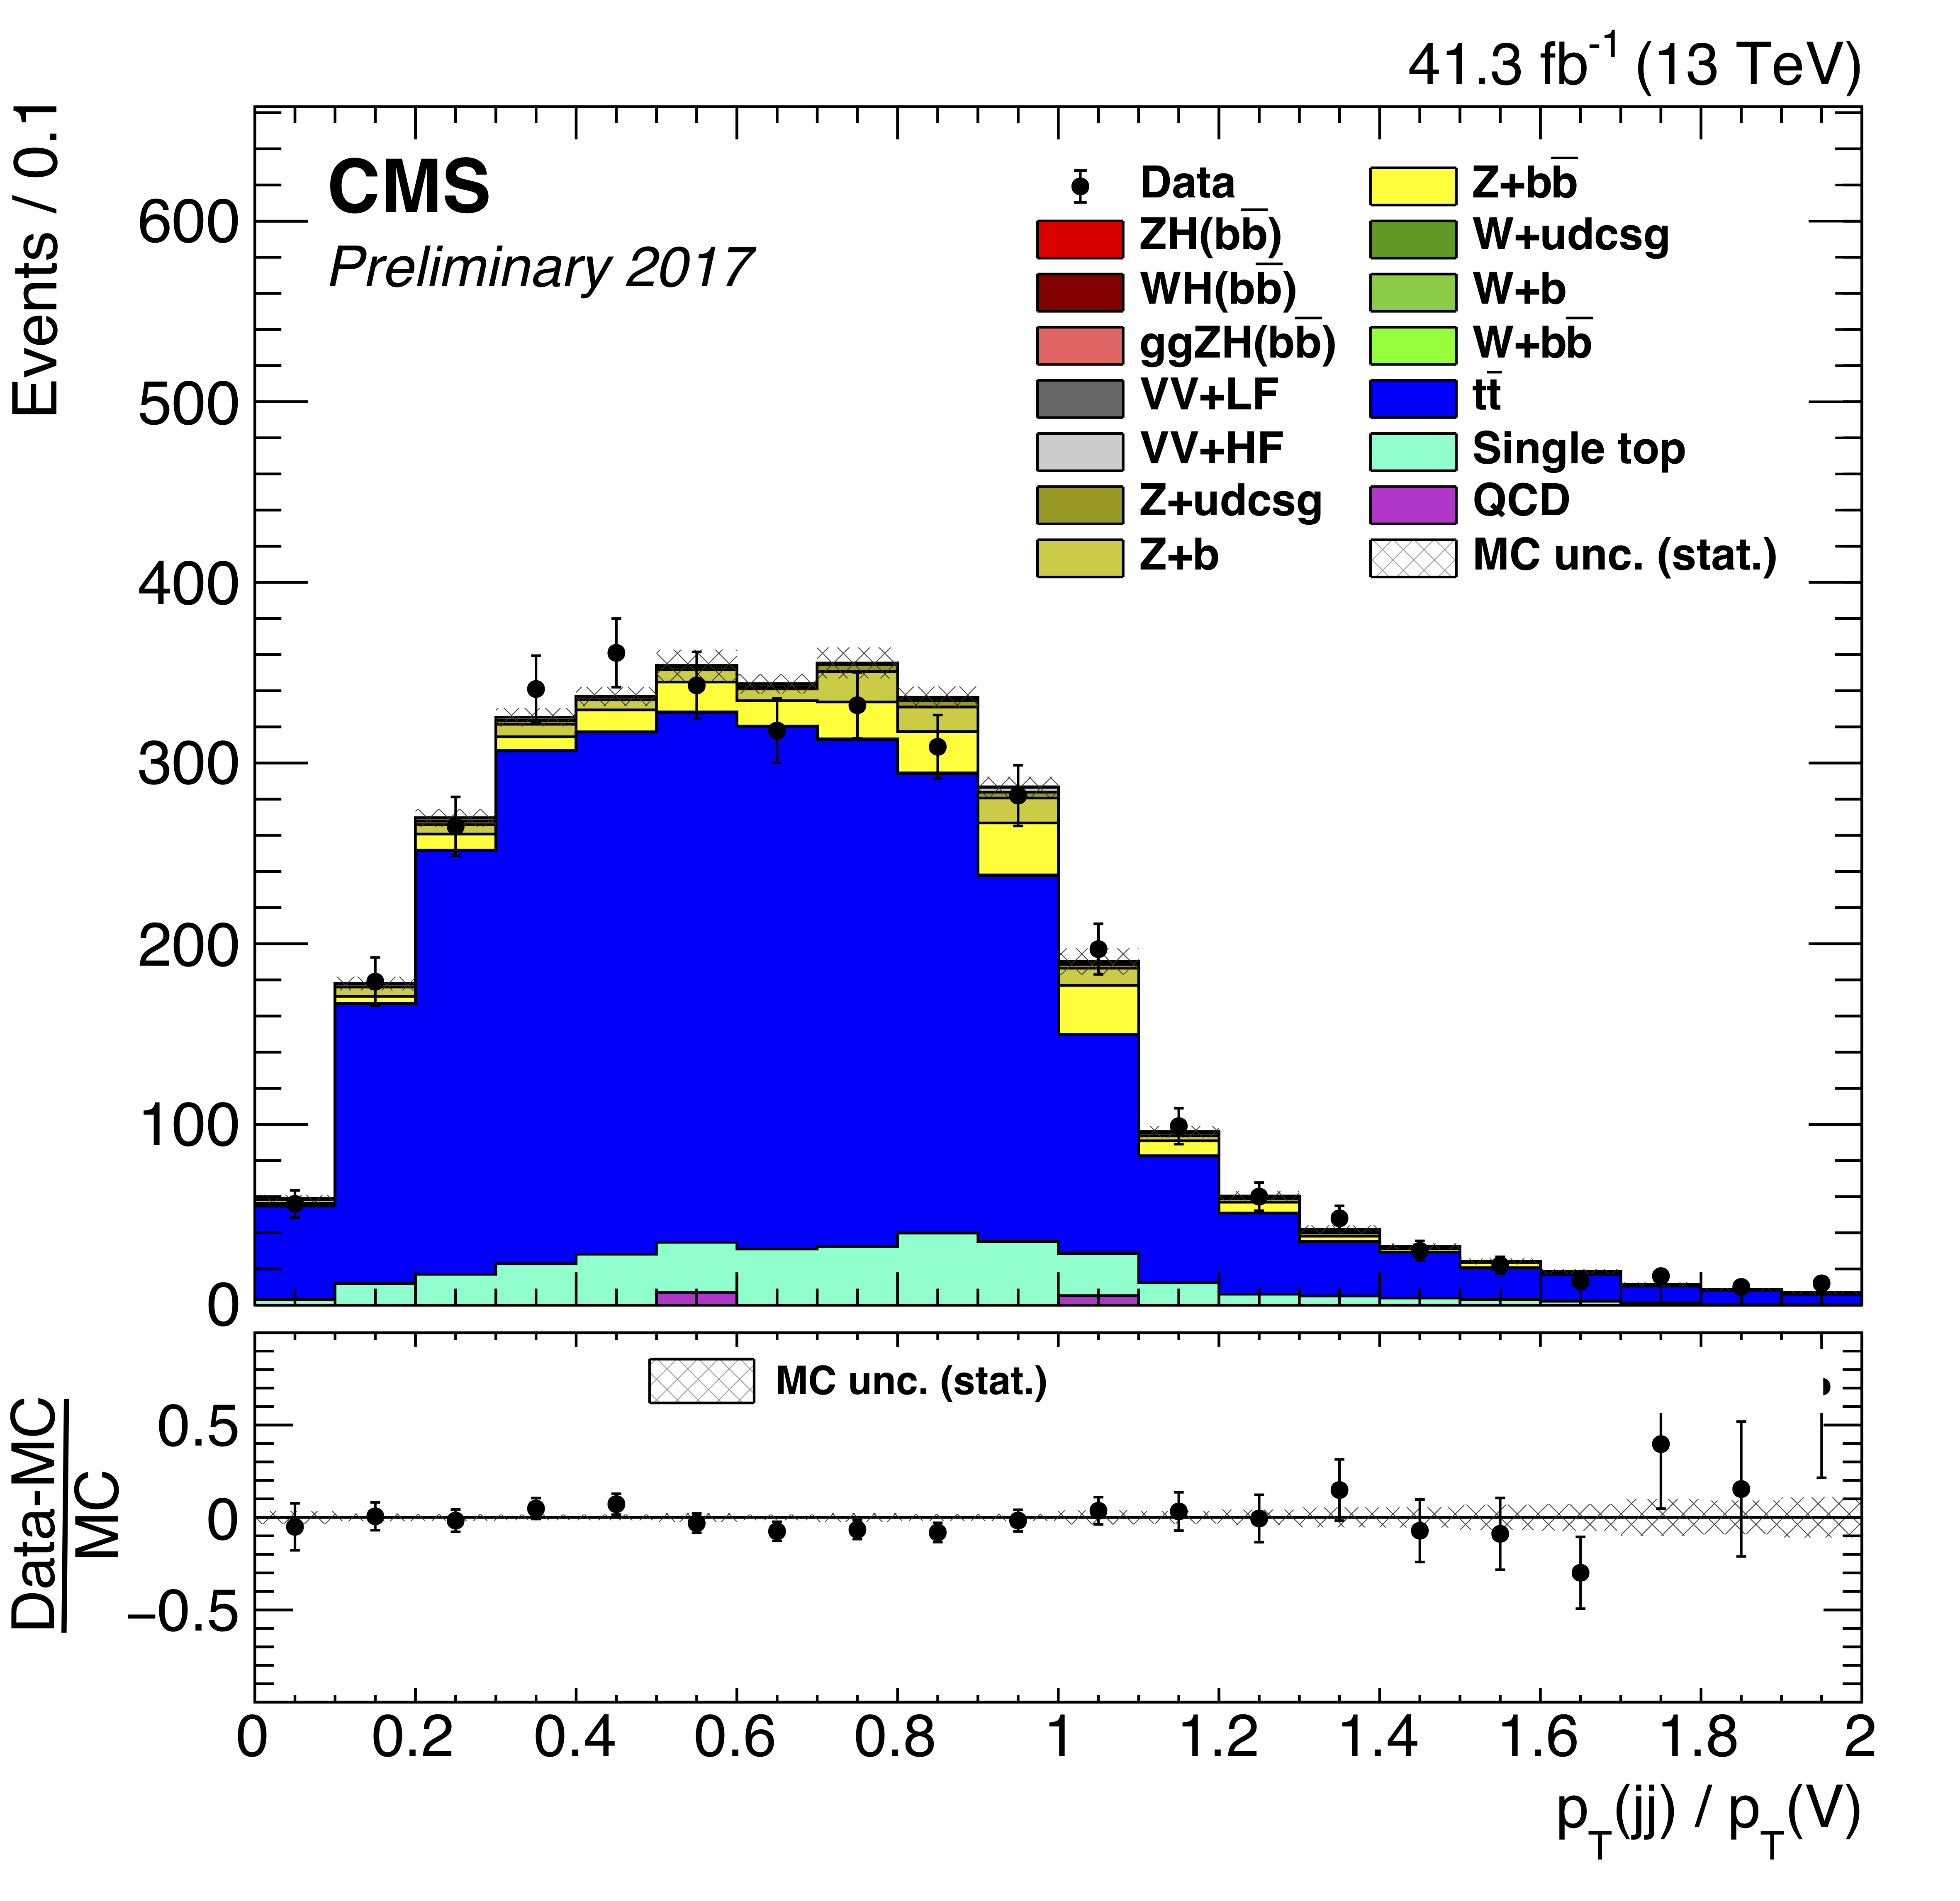
\includegraphics[width=0.39\linewidth]{images/CR_ZmmHighPt_TT/jjVPtRatio_fit}}
  }
  \mbox{
    \subfigure [] {\includegraphics[width=0.39\linewidth]{images/CR_ZeeHighPt_ZLF/H_mass_fit}}
    \subfigure [] {\includegraphics[width=0.39\linewidth]{images/CR_ZmmHighPt_ZLF/H_mass_fit}}
  }
  \mbox{
    \subfigure [] {\includegraphics[width=0.39\linewidth]{images/CR_ZeeHighPt_ZHF/hJets_DeepCSV_1}}
    \subfigure [] {\includegraphics[width=0.39\linewidth]{images/CR_ZmmHighPt_ZHF/hJets_DeepCSV_1}}
  }
  \caption[High $\pT(\bosV)$ Control Region Distributions for the \ZllH\ Channels]{The distributions of variables of the \ZeeH\ channel (left column) and the \ZmmH\ channel (right column) in the high $\pT(\bosV)$ region: A), B) $\pT(jj) / \pT(\bosV)$ for the \qrkt\qrktbar\ control region; C), D) $m(jj)$ for the \bosZ+light control region; E), F) \btagmin\ for the \bosZ+heavy control region.}
  \label{fig:CR_Zll_HighPt}
\end{figure}

\clearpage

%\clearpage %remove this command if your appendix doesn't start with a landscaped page!!!!!
%\thispagestyle{plain}
%\begin{landscape}
%\begin{figure}
 
%  \begin{center}
%    \includegraphics[width=6in]{images/LaTeX2e_logo.eps}
%    \caption{\LaTeX 2\ensuremath{\epsilon.} logo}\label{biglogo}
%  \end{center}
%\end{figure}
%\end{landscape}
 
 
%This is how a section should look if the first page is a landscape page.
%Lorem ipsum dolor sit amet, consectetuer adipiscing elit. Ut sit
%amet nulla. Integer mauris turpis, dapibus ac, auctor non, vehicula
%sit amet, magna. Suspendisse eu tellus. Etiam porta. Donec magna.
%Donec ut dui. In hac habitasse platea dictumst. Nullam suscipit, mi
%at adipiscing commodo, lorem erat scelerisque erat, non pulvinar leo
%mi eu metus. Phasellus id felis. Sed quam purus, molestie quis,
%ultrices nec, dictum at, magna. Proin viverra viverra ante.
